% Customizable fields and text areas start with % >> below.
% Lines starting with the comment character (%) are normally removed before release outside the collaboration, but not those comments ending lines

% svn info. These are modified by svn at checkout time.
% The last version of these macros found before the maketitle will be the one on the front page,
% so only the main file is tracked.
% Do not edit by hand!
\RCS$Revision: 391436 $
\RCS$HeadURL: svn+ssh://svn.cern.ch/reps/tdr2/notes/AN-17-029/trunk/AN-17-029.tex $
\RCS$Id: AN-17-029.tex 391436 2017-03-04 14:45:21Z peruzzi $
%%%%%%%%%%%%% local definitions %%%%%%%%%%%%%%%%%%%%%
% This allows for switching between one column and two column (cms@external) layouts
% The widths should  be modified for your particular figures. You'll need additional copies if you have more than one standard figure size.
\newlength\cmsFigWidth
\ifthenelse{\boolean{cms@external}}{\setlength\cmsFigWidth{0.85\columnwidth}}{\setlength\cmsFigWidth{0.4\textwidth}}
\ifthenelse{\boolean{cms@external}}{\providecommand{\cmsLeft}{top\xspace}}{\providecommand{\cmsLeft}{left\xspace}}
\ifthenelse{\boolean{cms@external}}{\providecommand{\cmsRight}{bottom\xspace}}{\providecommand{\cmsRight}{right\xspace}}
\newcommand{\ttH}{\ensuremath{\ttbar\PH}}
\newcommand{\ttZ}{\ensuremath{\ttbar\Z}}
\newcommand{\ttW}{\ensuremath{\ttbar\PW}}
\newcommand{\ttV}{\ensuremath{\ttbar\mathrm{V}}}
\newcommand{\Zll}{\ensuremath{\mathrm{Z}\to\ell^+\ell^-}\xspace}
\newcommand{\Ztt}{\ensuremath{\mathrm{Z}\to\tau^+\tau^-}\xspace}
\newcommand{\reliso}{\ensuremath{I_\mathrm{rel}}\xspace}
\newcommand{\sip}{\ensuremath{S_\mathrm{IP3D}}\xspace}
\newcommand{\Pgth}{\ensuremath{\Pgt_{\rm h}}\xspace}
\newcommand{\ptRatio}{\ensuremath{\pt^\text{ratio}}\xspace}
\newcommand{\ptRel}{\ensuremath{\pt^\text{rel}}\xspace}
\newcommand{\relIso}{\ensuremath{I_\text{rel}}\xspace}
\newcommand{\miniIso}{\ensuremath{I_\text{mini}}\xspace}

%%%%%%%%%%%%%%%  Title page %%%%%%%%%%%%%%%%%%%%%%%%
\cmsNoteHeader{AN-17-029} % This is over-written in the CMS environment: useful as preprint no. for export versions
% >> Title: please make sure that the non-TeX equivalent is in PDFTitle below
\title{Search for ttH in multilepton final states with the full 2016 dataset}

% >> Authors
%Author is always "The CMS Collaboration" for PAS and papers, so author, etc, below will be ignored in those cases
%For multiple affiliations, create an address entry for the combination
%To mark authors as primary, use the \author* form

\address[cern]{CERN}
\address[ndu]{University of Notre Dame}
\address[neb]{University of Nebraska}
\address[ihep]{IHEP}
\address[iphc]{IPHC}
\address[vub]{VUB}
\address[llr]{LLR}
\address[ovi]{University of Oviedo}

\author[iphc]{Daniel Bloch}
\author[cern]{Cristina Botta}
\author[iphc]{Nicolas Chanon}
\author[iphc]{Xavier Coubez}
\author[ndu]{Kevin Lannon}
\author[iphc]{Anne-Catherine Le Bihan}
\author[ihep]{Binghuan Li}
\author[iphc]{Jing Li}
\author[ndu]{Charlie Mueller}
\author[cern]{Marco Peruzzi}
\author[cern]{Giovanni Petrucciani}
\author[ihep]{Francesco Romeo}
\author[ovi]{Sergio Sanchez Cruz}
\author[vub]{Kirill Skovpen}
\author[ndu]{Geoffrey Smith}
\author[neb]{Benjamin Stieger}
\author[llr]{Thomas Strebler}
\author[ovi]{Pietro Vischia}
\author[ihep]{Huaqiao Zhang}


% >> Date
% The date is in yyyy/mm/dd format. Today has been
% redefined to match, but if the date needs to be fixed, please write it in this fashion.
% For papers and PAS, \today is taken as the date the head file (this one) was last modified according to svn: see the RCS Id string above.
% For the final version it is best to "touch" the head file to make sure it has the latest date.
\date{\today}

% >> Abstract
% Abstract processing:
% 1. **DO NOT use \include or \input** to include the abstract: our abstract extractor will not search through other files than this one.
% 2. **DO NOT use %**                  to comment out sections of the abstract: the extractor will still grab those lines (and they won't be comments any longer!).
% 3. For PASs: **DO NOT use tex macros**         in the abstract: CDS MathJax processor used on the abstract doesn't understand them _and_ will only look within $$. The abstracts for papers are hand formatted so macros are okay.
\abstract{A search for the standard model Higgs boson produced in association with a top quark pair is presented, using the full pp collision dataset collected by the CMS experiment in 2016. We target final states where the Higgs boson decays to either a W, Z or tau pair by selecting events with two isolated same-sign leptons, or more than three leptons, and b-jets.}

% >> PDF Metadata
% Do not comment out the following hypersetup lines (metadata). They will disappear in NODRAFT mode and are needed by CDS.
% Also: make sure that the values of the metadata items are sensible and are in plain text:
% (1) no TeX! -- for \sqrt{s} use sqrt(s) -- this will show with extra quote marks in the draft version but is okay).
% (2) no %.
% (3) No curly braces {}.
\hypersetup{%
pdfauthor={The ttH multilepton working group},%
pdftitle={Search for ttH in multilepton final states with the full 2016 dataset},%
pdfsubject={CMS},%
pdfkeywords={CMS, physics, higgs, top}}

\maketitle %maketitle comes after all the front information has been supplied
% >> Text
%%%%%%%%%%%%%%%%%%%%%%%%%%%%%%%%  Begin text %%%%%%%%%%%%%%%%%%%%%%%%%%%%%
%% **DO NOT REMOVE THE BIBLIOGRAPHY** which is located before the appendix.
%% You can take the text between here and the bibiliography as an example which you should replace with the actual text of your document.
%% If you include other TeX files, be sure to use "\input{filename}" rather than "\input filename".
%% The latter works for you, but our parser looks for the braces and will break when uploading the document.
%%%%%%%%%%%%%%%

\tableofcontents
\clearpage

\section{Introduction}
\label{sec:intro}
The LHC Run I data have been exploited to measure all the accessible
properties of the newly-discovered Higgs
boson\,\cite{cms_higgs,atlas_higgs}. ATLAS and CMS have combined their
effort in order to reach an already very precise measurement of the
boson mass, $125.09\pm 0.21\,(\mathrm{stat.})\,\pm 0.11\,(\mathrm{syst.})$
GeV\,\cite{atlas_cms_mass}. This precise mass result has created an
opportunity to test the predictions of the standard model by measuring
the other properties of the Higgs boson. Measurements of the Higgs boson production and decay rates and
constraints on its couplings have been performed by both
experiments~\cite{atlas_couplings,cms_couplings},
and, in general, agreement with the SM predictions given the current uncertainties
(10-30~$\%$) have been found. It is of great interest to use
the 13 TeV LHC data to further constrain these measurements, as any deviation from
expectation could be a sign of new physics.\\

Among these measurements, it is of particular interest to measure the coupling of the Higgs
boson to the top quark ($\ttbar \PH$) because the top quark
could play a special role in the context of electroweak symmetry
breaking due to its large mass.  The Higgs boson does not decay to top quarks. The
$\mathrm{t \bar t H}$ interaction vertex, however, is present in a
rare production mechanism where the Higgs boson is produced in
association with a top quark-antiquark pair as shown in
Fig.~\ref{fig:feyn}.  At LHC energies the largest contribution to the standard
model Higgs boson production is a gluon-gluon induced loop
dominated by virtual top exchange. The comparison of a direct
measurement of the $\ttbar \PH$ coupling with the one inferred from
the cross section measurement can put limits on the contribution of
new physics to the gluon-gluon loop.\\

The $\ttbar \PH$ process has been used by both ATLAS and CMS experiments to directly measure the
top-Higgs coupling at tree level with the 20~fb$^{-1}$ of 8~TeV
collisions of the LHC Run I. Via this process, both experiments reached a
30$\%$ accuracy on the top Yukawa coupling, a great achivement
given that the production cross section (130~fb at 8~TeV at
next-to-leading order (NLO)~\cite{YellowReport}) was two orders of magnitude
lower with respect to the dominant Higgs production mode (gluon-gluon
fusion). In order to achive this result several decay channels of the
Higgs boson have been considered by both experiments, and three main searches have
been designed. The first channel searches for
$\mathrm{t \bar t H}$ in events where the Higgs boson decays to
$\bbbar$; the best fit value for the combined signal strength obtained
by the CMS experiment is $0.7^{+1.9}_{-1.9}$ (95\%
CL))~\cite{cms_ttH}. The second channel searches 
for $\mathrm{t \bar t H}$ in events where the Higgs boson decays to
$\gamma \gamma$; the best fit value for the combined signal strength obtained
by the CMS experiment is $2.7^{+2.6}_{-1.8}$ (95\%
CL))~\cite{cms_ttH}. \\ 

We designed the third search to probe $\mathrm{t \bar t
H}$ events where the Higgs boson decays into $\mathrm{ZZ}^{*}$,
$\mathrm{WW}^{*}$, or $\tau\tau$, with at least one Z, W or $\tau$
decaying leptonically. Despite
the small branching ratio, the presence of one
or two additional leptons from the top quark pair decays leads to the
following clean experimental signatures:
%
\begin{itemize}
\item two same-sign leptons
(electrons or muons) plus b-tagged jets;
\item three leptons plus b-tagged jets;
\item four leptons plus b-tagged jets.
\end{itemize}
Examples of Feynman diagrams for $\mathrm{t \bar t H}$,
followed by the decays of the top quark and the Higgs boson that lead to the signatures
described above are shown  in Fig.\,\ref{fig:feyn}.
With this search we obtained the most precise measurement of the $\mathrm{t \bar t
H}$ signal strength: $3.7^{+1.9}_{-1.9}$
(95\%CL))~\cite{cms_multilepton}.\\

The combined best-fit signal strength
obtained assuming a Higgs boson mass of $125 \GeV$ was $\mu =
2.9^{+1.1}_{-0.9}$.  This result corresponds to a 3.5 standard
deviation excess over the background-only ($\mu = 0$) hypothesis, and
represents a 2.1 standard deviation upward fluctuation on the SM
$\ttbar \PH$ ($\mu = 1$) expectation. Although the combined observed signal strength is consistent with SM
expectations, with a roughly 2 standard deviation upward
fluctuation, it is interesting to point out that the excess was mainly
driven by the multilepton analysis, and in particular by the same-sign
di-muon subsample~\cite{cms_multilepton}.\\


With respect to 8~TeV, the 13~TeV $\mathrm{t \bar t H}$ cross section increased by a factor of 4 
with the higher center of mass energy, while the cross sections of the main backgrounds
$\ttbar\PW$, $\ttbar\Z$, $\ttbar$+jets increased by roughly a factor of 3.
We thus expect to increase our sensitivity during Run II, compared to Run I.

The first multilepton search at 13~TeV analyzed 2.3~fb$^{-1}$ of the 2015 dataset.
It measured the expected 95\% confidence level upper limit on the Higgs boson production cross section for a Higgs boson mass of 125 GeV/c$^2$
to be $2.6$ times the standard model expectation, compared to the observed limit of $3.3$.
The signal strength $\mu$, relative to the expectation for the standard model
Higgs boson, was measured to be $0.6_{-1.1}^{+1.4}$~\cite{cms_multilepton_2015}.\\

The 2016 data has been preliminarly analysed for the ICHEP conference considering 12.9~fb$^{-1}$ \cite{cms_multilepton_2016ICHEP}.
The results have been combined with the 2015 dataset and yield
a $\mathrm{t \bar t H}$ signal strength of $2.0_{-0.7}^{+0.8}$ times the standard model prediction.
They are used to set a 95\% confidence level upper limit on the signal production cross section of 3.4
times the standard model expectation, compared to an expected upper limit of $1.3_{-0.4}^{+0.6}$ in the absence of a signal.

In this note we perform the $\mathrm{t \bar t H}$ multilepton search with the full 2016 data, corresponding to 36.9 ~fb$^{-1}$,
collected by the CMS experiment at $\sqrt{s}$ = 13 TeV.
The general strategy remains similar to the previous searches.
Multivariate analysis techniques are used to identify objects with high purity and
to distinguish background from signal events.
The amount of signal is fit to the multivariate discriminant output distribution in all the final states simultaneously. \\

\begin{figure}[htb]
\centering
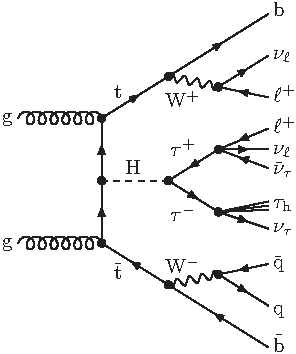
\includegraphics[width=0.30\linewidth]{diagrams/gg-ttH-tt-2lss.pdf} 
\hspace{0.5cm}
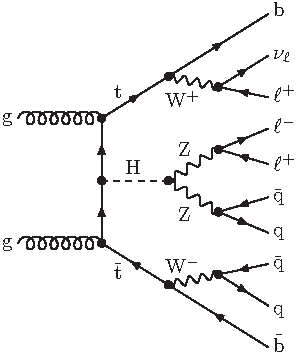
\includegraphics[width=0.30\linewidth]{diagrams/gg-ttH-ZZ-3l.pdf}
\hspace{0.5cm}
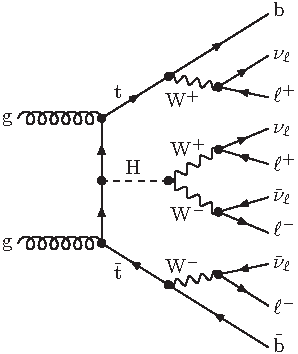
\includegraphics[width=0.30\linewidth]{diagrams/gg-ttH-WW-4l.pdf}
\caption{Examples of leading order Feynman diagrams for $t\bar{t}H$ production at pp colliders, with the Higgs boson decaying to
$\tau\tau$, $\mathrm{ZZ}^{*}$, and
$\mathrm{WW}^{*}$ (from left to right). The first, second, and third diagrams are examples of the two same-sign lepton signature,
the three lepton signature, and the four lepton signature, respectively.} 
\label{fig:feyn}
\end{figure}

\clearpage


\section{Data and MC Samples}
\label{sec:samples}
\subsection{Full 2016 dataset and MC samples}

The data considered in this analysis were collected by the CMS experiment during 2016 and correspond to a total integrated luminosity of 35.9\fbinv.
The data used were collected only in periods when the CMS magnet was on.
We use the 23 Sep 2016 (Run B to G) and PromptReco (Run H) versions of the datasets. 

The MC samples used in this analysis correspond to the RunIISummer16MiniAODv2 campaign produced with CMSSW 80X. 

The two signal samples (for \tHq\ and \tHW) were produced with \textsc{MG5\_}a\textsc{MC@NLO} (version 5.222), in leading-order order mode, and are normalized to next-to-leading-order cross sections, see Tab.~\ref{tab:sigsamples}.
Each sample is generated with a set of event weights corresponding to different values of \Ct\ and \CV\ couplings, see Tab.~\ref{tab:reweight}.

\begin{table}[h] 
  \centering
  \begin{tabular}{lll}
    Sample & $\sigma$ [pb] & BF \\
    \hline
    \verb|/THQ_Hincl_13TeV-madgraph-pythia8_TuneCUETP8M1/| & 0.7927 & 0.324 \\
    \verb|/THW_Hincl_13TeV-madgraph-pythia8_TuneCUETP8M1/| & 0.1472 & 1.0   \\
    \hline
  \end{tabular}
  \caption{Signal samples and their cross section and branching fraction used in this analysis. See Ref.~\cite{THQProdTwiki} for more details.}\label{tab:sigsamples}
\end{table}

\begin{table}[h!]
  \centering
  \footnotesize
  \begin{tabular}{lllllll}
        &       & \multicolumn{2}{c}{\tHq} & \multicolumn{2}{c}{\tHW} & \\\hline
   \CV\ & \Ct\  & sum of    & cross         & sum of    & cross        & \\
        &       & weights   & section [pb]  & weights   & section [pb] & LHE weights       \\\hline
   1.0  & -3.0  & 35.700022 & 2.991         & 11.030445 & 0.6409       & LHEweight\_wgt[446]\\
   1.0  & -2.0  & 20.124298 & 1.706         & 5.967205  & 0.3458       & LHEweight\_wgt[447]\\
   1.0  & -1.5  & 14.043198 & 1.205         & 4.029093  & 0.2353       & LHEweight\_wgt[448]\\
   1.0  & -1.25 & 11.429338 & 0.9869        & 3.208415  & 0.1876       & LHEweight\_wgt[449]\\
   1.0  & -1.0  &           & 0.7927        &           & 0.1472       & \\
   1.0  & -0.75 & 7.054998  & 0.6212        & 1.863811  & 0.1102       & LHEweight\_wgt[450]\\
   1.0  & -0.5  & 5.294518  & 0.4723        & 1.339886  & 0.07979      & LHEweight\_wgt[451]\\
   1.0  & -0.25 & 3.818499  & 0.3505        & 0.914880  & 0.05518      & LHEweight\_wgt[452]\\
   1.0  & 0.0   & 2.627360  & 0.2482        & 0.588902  & 0.03881      & LHEweight\_wgt[453]\\
   1.0  & 0.25  & 1.719841  & 0.1694        & 0.361621  & 0.02226      & LHEweight\_wgt[454]\\
   1.0  & 0.5   & 1.097202  & 0.1133        & 0.233368  & 0.01444      & LHEweight\_wgt[455]\\
   1.0  & 0.75  & 0.759024  & 0.08059       & 0.204034  & 0.01222      & LHEweight\_wgt[456]\\
   1.0  & 1.0   & 0.705305  & 0.07096       & 0.273617  & 0.01561      & LHEweight\_wgt[457]\\
   1.0  & 1.25  & 0.936047  & 0.0839        & 0.442119  & 0.02481      & LHEweight\_wgt[458]\\
   1.0  & 1.5   & 1.451249  & 0.1199        & 0.709538  & 0.03935      & LHEweight\_wgt[459]\\
   1.0  & 2.0   & 3.335034  & 0.2602        & 1.541132  & 0.08605      & LHEweight\_wgt[460]\\
   1.0  & 3.0   & 10.516125 & 0.8210        & 4.391335  & 0.2465       & LHEweight\_wgt[461]\\\hline
        &       &           &               &           &              & \\\hline
   1.5  & -3.0  & 45.281492 & 3.845         & 13.426212 & 0.7825       & LHEweight\_wgt[462]\\
   1.5  & -2.0  & 27.606715 & 2.371         & 7.809713  & 0.4574       & LHEweight\_wgt[463]\\
   1.5  & -1.5  & 20.476088 & 1.784         & 5.594971  & 0.3290       & LHEweight\_wgt[464]\\
   1.5  & -1.25 & 17.337465 & 1.518         & 4.635978  & 0.2749       & LHEweight\_wgt[465]\\
   1.5  & -1.0  & 14.483302 & 1.287         & 3.775902  & 0.2244       & LHEweight\_wgt[466]\\
   1.5  & -0.75 & 11.913599 & 1.067         & 3.014744  & 0.1799       & LHEweight\_wgt[467]\\
   1.5  & -0.5  & 9.628357  & 0.874         & 2.352505  & 0.1410       & LHEweight\_wgt[468]\\
   1.5  & -0.25 & 7.627574  & 0.702         & 1.789184  & 0.1081       & LHEweight\_wgt[469]\\
   1.5  & 0.0   & 5.911882  & 0.5577        & 1.324946  & 0.08056      & LHEweight\_wgt[470]\\
   1.5  & 0.25  & 4.479390  & 0.4365        & 0.959295  & 0.05893      & LHEweight\_wgt[471]\\
   1.5  & 0.5   & 3.331988  & 0.3343        & 0.692727  & 0.04277      & LHEweight\_wgt[472]\\
   1.5  & 0.75  & 2.469046  & 0.2558        & 0.525078  & 0.03263      & LHEweight\_wgt[473]\\
   1.5  & 1.0   & 1.890565  & 0.2003        & 0.456347  & 0.02768      & LHEweight\_wgt[474]\\
   1.5  & 1.25  & 1.596544  & 0.1689        & 0.486534  & 0.02864      & LHEweight\_wgt[475]\\
   1.5  & 1.5   & 1.586983  & 0.1594        & 0.615638  & 0.03509      & LHEweight\_wgt[476]\\
   1.5  & 2.0   & 2.421241  & 0.2105        & 1.170602  & 0.06515      & LHEweight\_wgt[477]\\
   1.5  & 3.0   & 7.503280  & 0.5889        & 3.467546  & 0.1930       & LHEweight\_wgt[478]\\\hline
        &       &           &               &           & \\ \hline
   0.5  & -3.0  & 27.432685 & 2.260         & 8.929074  & 0.5136       & LHEweight\_wgt[479]\\
   0.5  & -2.0  & 13.956013 & 1.160         & 4.419093  & 0.2547       & LHEweight\_wgt[480]\\
   0.5  & -1.5  & 8.924438  & 0.7478        & 2.757611  & 0.1591       & LHEweight\_wgt[481]\\
   0.5  & -1.25 & 6.835341  & 0.5726        & 2.075247  & 0.1204       & LHEweight\_wgt[482]\\
   0.5  & -1.0  & 5.030704  & 0.4273        & 1.491801  & 0.08696      & LHEweight\_wgt[483]\\
   0.5  & -0.75 & 3.510528  & 0.2999        & 1.007273  & 0.05885      & LHEweight\_wgt[484]\\
   0.5  & -0.5  & 2.274811  & 0.1982        & 0.621663  & 0.03658      & LHEweight\_wgt[485]\\
   0.5  & -0.25 & 1.323555  & 0.1189        & 0.334972  & 0.01996      & LHEweight\_wgt[486]\\
   0.5  & 0.0   & 0.656969  & 0.06223       & 0.147253  & 0.008986     & LHEweight\_wgt[487]\\
   0.5  & 0.25  & 0.274423  & 0.02830       & 0.058342  & 0.003608     & LHEweight\_wgt[488]\\
   0.5  & 0.5   & 0.176548  & 0.01778       & 0.068404  & 0.003902     & LHEweight\_wgt[489]\\
   0.5  & 0.75  & 0.363132  & 0.03008       & 0.177385  & 0.009854     & LHEweight\_wgt[490]\\
   0.5  & 1.0   & 0.834177  & 0.06550       & 0.385283  & 0.02145      & LHEweight\_wgt[491]\\
   0.5  & 1.25  & 1.589682  & 0.1241        & 0.692099  & 0.03848      & LHEweight\_wgt[492]\\
   0.5  & 1.5   & 2.629647  & 0.2047        & 1.097834  & 0.06136      & LHEweight\_wgt[493]\\
   0.5  & 2.0   & 5.562958  & 0.4358        & 2.206057  & 0.1246       & LHEweight\_wgt[494]\\
   0.5  & 3.0   & 14.843102 & 1.177         & 5.609519  & 0.3172       & LHEweight\_wgt[495]\\ \hline
    \end{tabular} 
    \caption{\CV\ and \Ct\ combinations generated for the two signal samples and their NLO cross sections. The \tHq\ cross section is multiplied by the branching fraction of the enforced leptonic decay of the top quark (0.324). See also Ref.~\cite{THQProdTwiki}.}\label{tab:reweight}
 \end{table}

Different MC generators were used to generate the background processes.
The dominant sources (\ttbar, \ttW, \ttZ, \ttH) were produced using \textsc{aMC@NLO} interfaced to \PYTHIA8, and are scaled to NLO cross sections.
Other processes are simulated using \POWHEG\ interfaced to \PYTHIA, or bare \PYTHIA.
See table~\ref{tab:bgsamples} for more details.
See also AN-2016-211 (Ref.~\cite{CMS_AN_2016-211}) for more details.

\begin{table}
\footnotesize
\centering
\begin{tabular}{ll}
	Sample & $\sigma$ [pb] \\
	\hline
	\verb|TTWJetsToLNu_TuneCUETP8M1_13TeV-amcatnloFXFX-madspin-pythia8|           & 0.2043 \\
	\verb|TTZToLLNuNu_M-10_TuneCUETP8M1_13TeV-amcatnlo-pythia8|                   & 0.2529 \\
	\verb|ttHJetToNonbb_M125_13TeV_amcatnloFXFX_madspin_pythia8_mWCutfix|         & 0.2151 \\
	\verb|/store/cmst3/group/susy/gpetrucc/13TeV/u/TTLL_m1to10_LO_NoMS_for76X/|   & 0.0283 \\
	\verb|WGToLNuG_TuneCUETP8M1_13TeV-madgraphMLM-pythia8|                        & 585.8 \\
	\verb|ZGTo2LG_TuneCUETP8M1_13TeV-amcatnloFXFX-pythia8|                        & 131.3 \\
	\verb|TGJets_TuneCUETP8M1_13TeV_amcatnlo_madspin_pythia8|                     & 2.967 \\
	\verb|TTGJets_TuneCUETP8M1_13TeV-amcatnloFXFX-madspin-pythia8|                & 3.697 \\
	\verb|WpWpJJ_EWK-QCD_TuneCUETP8M1_13TeV-madgraph-pythia8|                     & 0.03711 \\
	\verb|ZZZ_TuneCUETP8M1_13TeV-amcatnlo-pythia8|                                & 0.01398 \\
	\verb|WWZ_TuneCUETP8M1_13TeV-amcatnlo-pythia8|                                & 0.1651 \\
	\verb|WZZ_TuneCUETP8M1_13TeV-amcatnlo-pythia8|                                & 0.05565 \\
	\verb|WW_DoubleScattering_13TeV-pythia8|                                      & 1.64 \\
	\verb|tZq_ll_4f_13TeV-amcatnlo-pythia8_TuneCUETP8M1|                          & 0.0758 \\
	\verb|ST_tWll_5f_LO_13TeV-MadGraph-pythia8|                                   & 0.01123 \\
	\verb|TTTT_TuneCUETP8M1_13TeV-amcatnlo-pythia8|                               & 0.009103 \\
	\verb|WZTo3LNu_TuneCUETP8M1_13TeV-powheg-pythia8|                             & 4.4296 \\
	\verb|ZZTo4L_13TeV_powheg_pythia8|                                            & 1.256 \\
	\hline
	\verb|TTJets_SingleLeptFromTbar_TuneCUETP8M1_13TeV-madgraphMLM-pythia8|       & 182.1754 \\
	\verb|TTJets_SingleLeptFromT_TuneCUETP8M1_13TeV-madgraphMLM-pythia8|          & 182.1754 \\
	\verb|TTJets_DiLept_TuneCUETP8M1_13TeV-madgraphMLM-pythia8|                   & 87.3 \\
	\verb|DYJetsToLL_M-10to50_TuneCUETP8M1_13TeV-amcatnloFXFX-pythia8|            & 18610 \\
	\verb|DYJetsToLL_M-50_TuneCUETP8M1_13TeV-madgraphMLM-pythia8|                 & 6024 \\
	\verb|WJetsToLNu_TuneCUETP8M1_13TeV-amcatnloFXFX-pythia8|                     & 61526.7 \\
	\verb|ST_tW_top_5f_inclusiveDecays_13TeV-powheg-pythia8_TuneCUETP8M1|         & 35.6 \\
	\verb|ST_tW_antitop_5f_inclusiveDecays_13TeV-powheg-pythia8_TuneCUETP8M1|     & 35.6 \\
	\verb|ST_t-channel_4f_leptonDecays_13TeV-amcatnlo-pythia8_TuneCUETP8M1|       & 70.3144\\
	\verb|ST_t-channel_antitop_4f_leptonDecays_13TeV-powheg-pythia8_TuneCUETP8M1| & 26.2278\\
	\verb|ST_s-channel_4f_leptonDecays_13TeV-amcatnlo-pythia8_TuneCUETP8M1|       & 3.68064 \\
	\verb|WWTo2L2Nu_13TeV-powheg|                                                 & 10.481 \\
	\hline
\end{tabular}
\caption{List of background samples used in this analysis (CMSSW
  80X). In the first section of the table are listed the samples of
  the processes for which we use the simulation to extract the final
  yields and shapes, in the second section the samples of the
  processes we will estimate from data. The MC simulation is used to
  design the data driven methods and derive the associated systematics.} \label{tab:bgsamples}
\end{table}

\begin{table}
\centering
\begin{tabular}{ll}
	Sample & $\sigma$ [pb] \\
	\hline
	\verb|ttWJets_13TeV_madgraphMLM| & 0.6105 \\
	\verb|ttZJets_13TeV_madgraphMLM| & 0.5297/0.692 \\
	\hline
\end{tabular}
\caption{Leading-order \ttW\ and \ttZ\ samples used in the signal BDT training.} \label{tab:ttvlo_samples}
\end{table}

\subsection{Triggers}
We consider online-reconstructed events triggered by one, two, or three leptons.
Single-lepton triggers are included to boost the acceptance of events where the \pt\ of the sub-leading lepton falls below the threshold of the double-lepton triggers.
Additionally, by including double-lepton triggers in the $\geq$ 3 lepton category, as well as single-lepton triggers in all categories, we increase the efficiency, considering the logical ``or'' of the trigger decisions of all the individual triggers in a given category.
Tab.~\ref{tab:triggers} shows the lowest-threshold non-prescaled triggers present in the High-Level Trigger (HLT) menus for both Monte-Carlo and data in 2016.

\begin{table}[h]
\centering
	\begin{tabular}{l}
    \hline
    Same-sign dilepton (==2 muons)\\
    \verb|HLT_Mu17_TrkIsoVVL_Mu8_TrkIsoVVL_DZ_v*|\\
    \verb|HLT_Mu17_TrkIsoVVL_TkMu8_TrkIsoVVL_DZ_v*|\\
    \verb|HLT_IsoMu22_v*|\\
    \verb|HLT_IsoTkMu22_v*|\\
    \verb|HLT_IsoMu22_eta2p1_v*| \\
    \verb|HLT_IsoTkMu22_eta2p1_v*| \\
    \verb|HLT_IsoMu24_v*| \\
    \verb|HLT_IsoTkMu24_v*|\\\hline
    Same-sign dilepton (==2 electrons)\\
    \verb|HLT_Ele23_Ele12_CaloIdL_TrackIdL_IsoVL_DZ_v*|\\
    \verb|HLT_Ele27_eta2p1_WPLoose_Gsf_v*|\\
    \verb|HLT_Ele27_WPTight_Gsf_v*| \\
    \verb|HLT_Ele25_eta2p1_WPTight_Gsf_v*| \\\hline
    Same-sign dilepton (==1 muon, ==1 electron)\\
    \verb|HLT_Mu23_TrkIsoVVL_Ele8_CaloIdL_TrackIdL_IsoVL_v*|\\
    \verb|HLT_Mu8_TrkIsoVVL_Ele23_CaloIdL_TrackIdL_IsoVL_v*|\\
    \verb|HLT_Mu23_TrkIsoVVL_Ele8_CaloIdL_TrackIdL_IsoVL_DZ_v*| \\
    \verb|HLT_Mu8_TrkIsoVVL_Ele23_CaloIdL_TrackIdL_IsoVL_DZ_v*| \\
    \verb|HLT_IsoMu22_v*|\\
    \verb|HLT_IsoTkMu22_v*|\\
    \verb|HLT_IsoMu22_eta2p1_v*| \\
    \verb|HLT_IsoTkMu22_eta2p1_v*| \\
    \verb|HLT_IsoMu24_v*| \\
    \verb|HLT_IsoTkMu24_v*| \\
    \verb|HLT_Ele27_WPTight_Gsf_v*| \\
    \verb|HLT_Ele25_eta2p1_WPTight_Gsf_v*| \\
    \verb|HLT_Ele27_eta2p1_WPLoose_Gsf_v*|\\\hline
    Three lepton and Four lepton\\
    \verb|HLT_DiMu9_Ele9_CaloIdL_TrackIdL_v*|\\
    \verb|HLT_Mu8_DiEle12_CaloIdL_TrackIdL_v*|\\
    \verb|HLT_TripleMu_12_10_5_v*|\\
    \verb|HLT_Ele16_Ele12_Ele8_CaloIdL_TrackIdL_v*|\\
    \verb|HLT_Mu23_TrkIsoVVL_Ele8_CaloIdL_TrackIdL_IsoVL_v*|\\
    \verb|HLT_Mu23_TrkIsoVVL_Ele8_CaloIdL_TrackIdL_IsoVL_DZ_v*| \\
    \verb|HLT_Mu8_TrkIsoVVL_Ele23_CaloIdL_TrackIdL_IsoVL_v*|\\
    \verb|HLT_Mu8_TrkIsoVVL_Ele23_CaloIdL_TrackIdL_IsoVL_DZ_v|* \\
    \verb|HLT_Ele23_Ele12_CaloIdL_TrackIdL_IsoVL_DZ_v*|\\
    \verb|HLT_Mu17_TrkIsoVVL_Mu8_TrkIsoVVL_DZ_v*|\\
    \verb|HLT_Mu17_TrkIsoVVL_TkMu8_TrkIsoVVL_DZ_v*|\\
    \verb|HLT_IsoMu22_v*|\\
    \verb|HLT_IsoTkMu22_v*|\\
    \verb|HLT_IsoMu22_eta2p1_v*|\\
    \verb|HLT_IsoTkMu22_eta2p1_v*|\\
    \verb|HLT_IsoMu24_v*|\\
    \verb|HLT_IsoTkMu24_v*|\\
    \verb|HLT_Ele27_WPTight_Gsf_v*|\\
    \verb|HLT_Ele25_eta2p1_WPTight_Gsf_v*|\\
    \verb|HLT_Ele27_eta2p1_WPLoose_Gsf_v*|\\
	\hline
    \end{tabular}
    \caption{Table of high-level triggers that we consider in the analysis.} \label{tab:triggers}
\end{table}

\subsubsection{Trigger efficiency scale factors}
The efficiency of events to pass the trigger is measured in simulation (trivially using generator information) and in the data (using event collected by an uncorrelated MET trigger).
Small differences between the data and MC efficiencies are corrected by applying scale factors as shown in Tab.~\ref{tab:trigSFs}.
The exact procedure and control plots are documented in Refs~\cite{CMS_AN_2016-211} (for the ICHEP dataset), and in~\cite{CMS_AN_2017-029} for the current analysis.

\begin{table}
\centering
\begin{tabular}{ll}
	Category & Scale Factor \\
	\hline
	ee       & $1.01 \pm 0.02$ \\
	e$\mu$   & $1.01 \pm 0.01$ \\
	$\mu\mu$ & $1.00 \pm 0.01$ \\
	3l       & $1.00 \pm 0.03$ \\
	\hline
\end{tabular}
\caption{Trigger efficiency scale factors and associated uncertainties, shown here rounded to the nearest percent.}
\label{tab:trigSFs}
\end{table}

%\usepackage[usenames, dvipsnames]{color}
\subsection{Triggers}
\label{sec:trigger}

In this analysis, we consider online-reconstructed events triggered on one, two or three leptons. The inclusion of single-lepton triggers 
boosts acceptance by including events where the \pt of the subleading lepton falls below the threshold of the double-lepton triggers.
In addition, by including double-lepton triggers in the $\geq 3$ lepton category, as well as single-lepton triggers in all categories, 
we increase efficiency by considering the logical ``or" of the trigger decisions of all the individual triggers in a given category. 
Table~\ref{tab:triggers} shows the lowest-threshold unprescaled triggers present in the High-Level Trigger (HLT) menus for both 
Monte-Carlo and data in 2016 (will be updated if subsequent data have different unprescaled triggers).\\

\begin{table}[h]
\footnotesize
\centering
\begin{tabular}{l}
\hline
Same-sign dilepton (==2 muons) \\
\hline
HLT\_Mu17\_TrkIsoVVL\_Mu8\_TrkIsoVVL\_DZ\_v* \\
HLT\_Mu17\_TrkIsoVVL\_TkMu8\_TrkIsoVVL\_DZ\_v* \\
HLT\_IsoMu22\_v* \\
HLT\_IsoTkMu22\_v* \\
HLT\_IsoMu22\_eta2p1\_v* \\
HLT\_IsoTkMu22\_eta2p1\_v* \\
HLT\_IsoMu24\_v* \\
HLT\_IsoTkMu24\_v* \\
\hline
\hline
Same-sign dilepton (==2 electrons) \\
\hline
HLT\_Ele23\_Ele12\_CaloIdL\_TrackIdL\_IsoVL\_DZ\_v* \\
HLT\_Ele27\_WPTight\_Gsf\_v* \\
HLT\_Ele25\_eta2p1\_WPTight\_Gsf\_v* \\
HLT\_Ele27\_eta2p1\_WPLoose\_Gsf\_v* \\
\hline
\hline
Same-sign dilepton (==1 muon, ==1 electron) \\
\hline
HLT\_Mu23\_TrkIsoVVL\_Ele8\_CaloIdL\_TrackIdL\_IsoVL\_v* \\
HLT\_Mu23\_TrkIsoVVL\_Ele8\_CaloIdL\_TrackIdL\_IsoVL\_DZ\_v* \\
HLT\_Mu8\_TrkIsoVVL\_Ele23\_CaloIdL\_TrackIdL\_IsoVL\_v* \\
HLT\_Mu8\_TrkIsoVVL\_Ele23\_CaloIdL\_TrackIdL\_IsoVL\_DZ\_v* \\
HLT\_IsoMu22\_v* \\
HLT\_IsoTkMu22\_v* \\
HLT\_IsoMu22\_eta2p1\_v* \\
HLT\_IsoTkMu22\_eta2p1\_v* \\
HLT\_IsoMu24\_v* \\
HLT\_IsoTkMu24\_v* \\
HLT\_Ele27\_WPTight\_Gsf\_v* \\
HLT\_Ele25\_eta2p1\_WPTight\_Gsf\_v* \\
HLT\_Ele27\_eta2p1\_WPLoose\_Gsf\_v* \\
\hline
\hline
Three lepton and Four lepton \\
\hline
HLT\_DiMu9\_Ele9\_CaloIdL\_TrackIdL\_v* \\
HLT\_Mu8\_DiEle12\_CaloIdL\_TrackIdL\_v* \\
HLT\_TripleMu\_12\_10\_5\_v* \\
HLT\_Ele16\_Ele12\_Ele8\_CaloIdL\_TrackIdL\_v* \\
HLT\_Mu23\_TrkIsoVVL\_Ele8\_CaloIdL\_TrackIdL\_IsoVL\_v* \\
HLT\_Mu23\_TrkIsoVVL\_Ele8\_CaloIdL\_TrackIdL\_IsoVL\_DZ\_v* \\
HLT\_Mu8\_TrkIsoVVL\_Ele23\_CaloIdL\_TrackIdL\_IsoVL\_v* \\
HLT\_Mu8\_TrkIsoVVL\_Ele23\_CaloIdL\_TrackIdL\_IsoVL\_DZ\_v* \\
HLT\_Ele23\_Ele12\_CaloIdL\_TrackIdL\_IsoVL\_DZ\_v* \\
HLT\_Mu17\_TrkIsoVVL\_Mu8\_TrkIsoVVL\_DZ\_v* \\
HLT\_Mu17\_TrkIsoVVL\_TkMu8\_TrkIsoVVL\_DZ\_v* \\
HLT\_IsoMu22\_v* \\
HLT\_IsoTkMu22\_v* \\
HLT\_IsoMu22\_eta2p1\_v* \\
HLT\_IsoTkMu22\_eta2p1\_v* \\
HLT\_IsoMu24\_v* \\
HLT\_IsoTkMu24\_v* \\
HLT\_Ele27\_WPTight\_Gsf\_v* \\
HLT\_Ele25\_eta2p1\_WPTight\_Gsf\_v* \\
HLT\_Ele27\_eta2p1\_WPLoose\_Gsf\_v* \\
\hline
\end{tabular}
\caption{Table of high-level triggers that we consider in the analysis.}
\label{tab:triggers}
\end{table}

Figures~\ref{fig:trigeffsmumu}, \ref{fig:trigeffsemu}, \ref{fig:trigeffsee}, 
and \ref{fig:trigeffs3l} show a comparison of the trigger efficiency
between data and Monte-Carlo in each of the analysis categories.
In general, we find that the trigger efficiencies in the data agree well with
simulation. Measuring the efficiency in simulated
events is straightforward because there is no trigger bias with simulated
events. To measure the efficiency in data we follow the procedure
described here~\cite{CMS-AN-12-389}, which was also the same procedure 
used in the Run I, 2015 Run II, and 2016 Run II (ICHEP) multilepton analyses. We first select a
set of events that were recorded on a trigger that is uncorrelated
with the lepton triggers. We use events recorded on a
MET trigger as a unbiased sample. We then look for candidate events
with exactly two good leptons (and separately, events with exactly three good leptons). We measure the efficiency for the
candidate events to pass the logical ``or" of triggers being considered
in a given event category (i.e., the triggers listed by category in table~\ref{tab:triggers}). \\

We use scale factors to correct for small differences in the trigger efficiency
between data and Monte-Carlo. We compare the efficiency measured in data to the
efficiency in simulation, and derive correction factors which are the ratio of
these two efficiencies. Overall, we see good agreement between the efficiency in data and 
the efficiency in simulation, so we apply a flat scale factor close to unity in each category. 
These scale factors are summarized in table~\ref{tab:trigSFs}.


%Some of our Monte-Carlo samples were not produced with trigger information. For these
%samples, as well as applying the data/MC trigger scale factors, we also apply a per-event weight based
%on the trigger efficiency measured in ttH Monte-Carlo. These 
%weights are binned in 2 dimensions as a function of the leading and subleading lepton \pt.
%Figure~\ref{fig:trigeffsWeights} summarizes these efficiencies. As a cross-check, we 
%compare the shapes of a variety of event variables after applying the efficiencies in figure~\ref{fig:trigeffsWeights},
%versus after filtering directly from the trigger decisions. We observe good agreement
%between the two methods for each of these variables, 
%including the \pt of the dilepton system (made up of the two
%leading leptons), shown in Figure~\ref{fig:trigClosure}. 

\begin{figure}[htp]
\centering
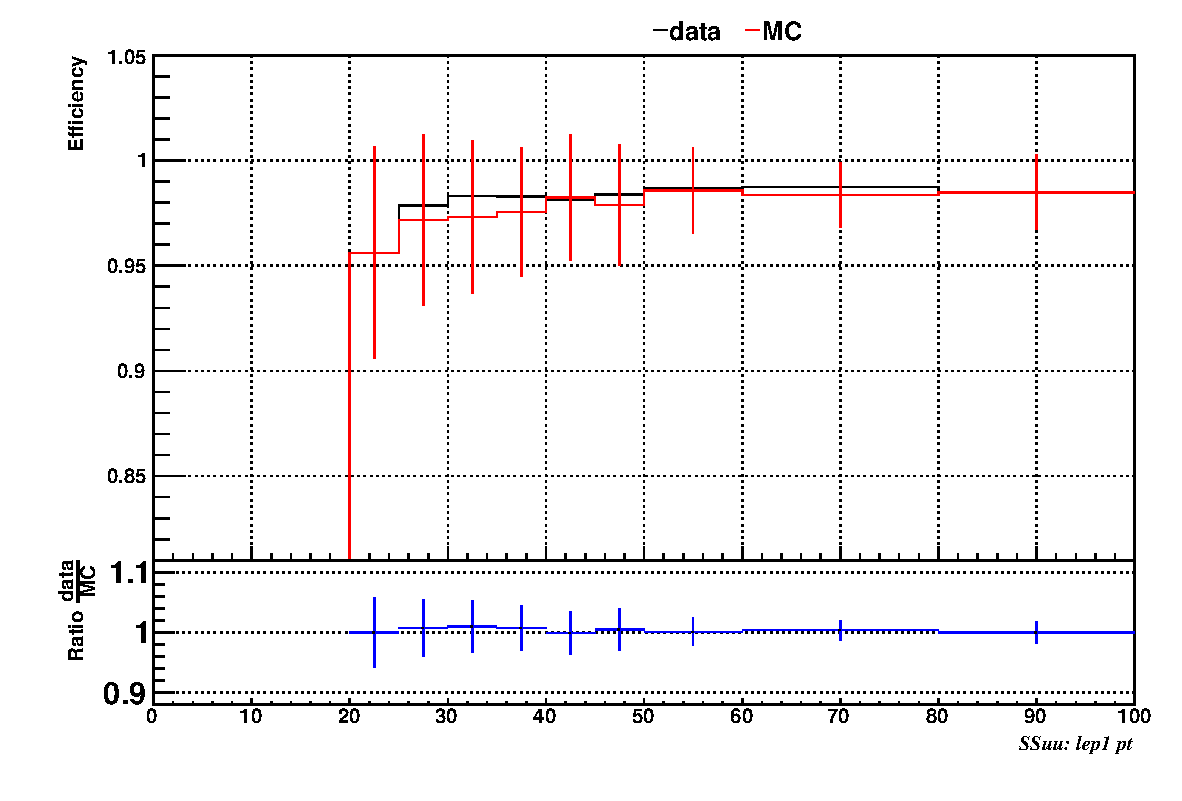
\includegraphics[width=0.49\textwidth]{plots_trigger/1D_eff_lep1_pt_uu_ARCv2_change_3l_pt_ranges.pdf}
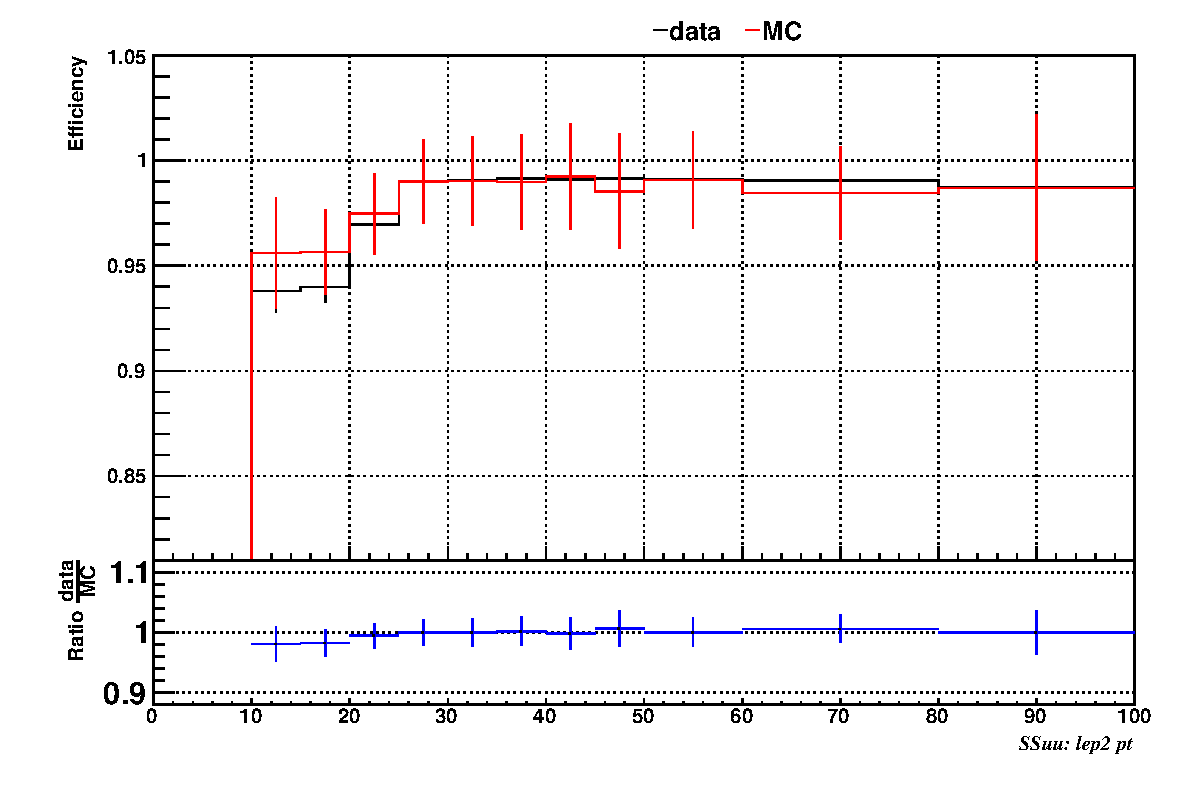
\includegraphics[width=0.49\textwidth]{plots_trigger/1D_eff_lep2_pt_uu_ARCv2_change_3l_pt_ranges.pdf} \\
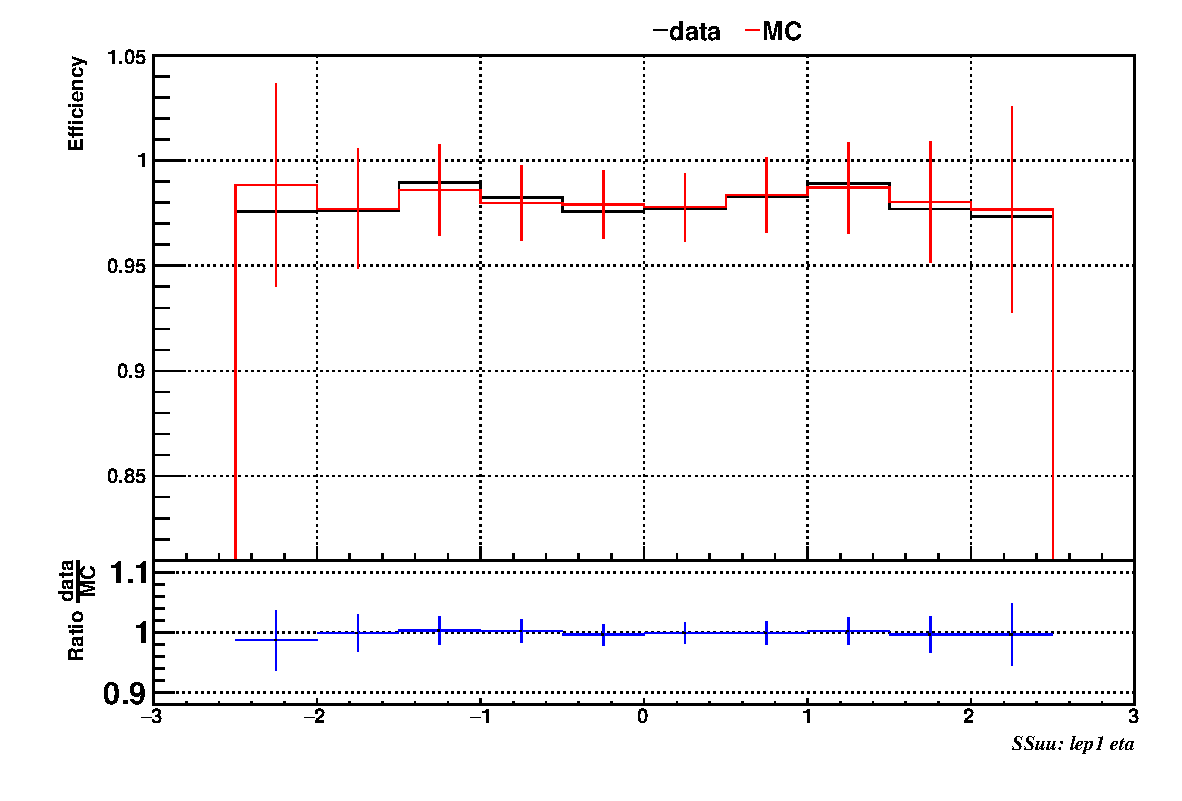
\includegraphics[width=0.49\textwidth]{plots_trigger/1D_eff_lep1_eta_uu_ARCv2_change_3l_pt_ranges.pdf}
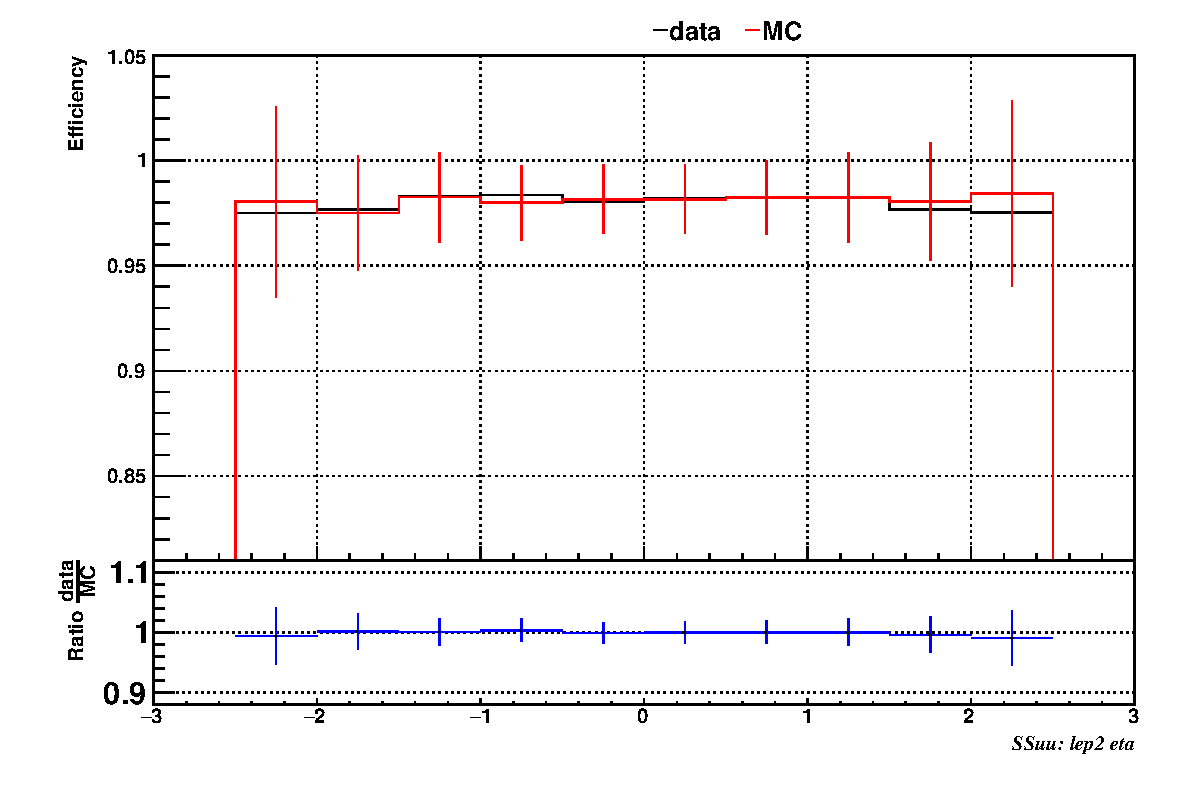
\includegraphics[width=0.49\textwidth]{plots_trigger/1D_eff_lep2_eta_uu_ARCv2_change_3l_pt_ranges.pdf}
\caption{Comparison of the trigger efficiency in the same-sign dimuon category before 
corrections, shown as a function of the \pt and $\eta$ of the leading lepton (left) 
and the sub-leading lepton (right).}
\label{fig:trigeffsmumu}
\end{figure}

\begin{figure}[htp]
\centering
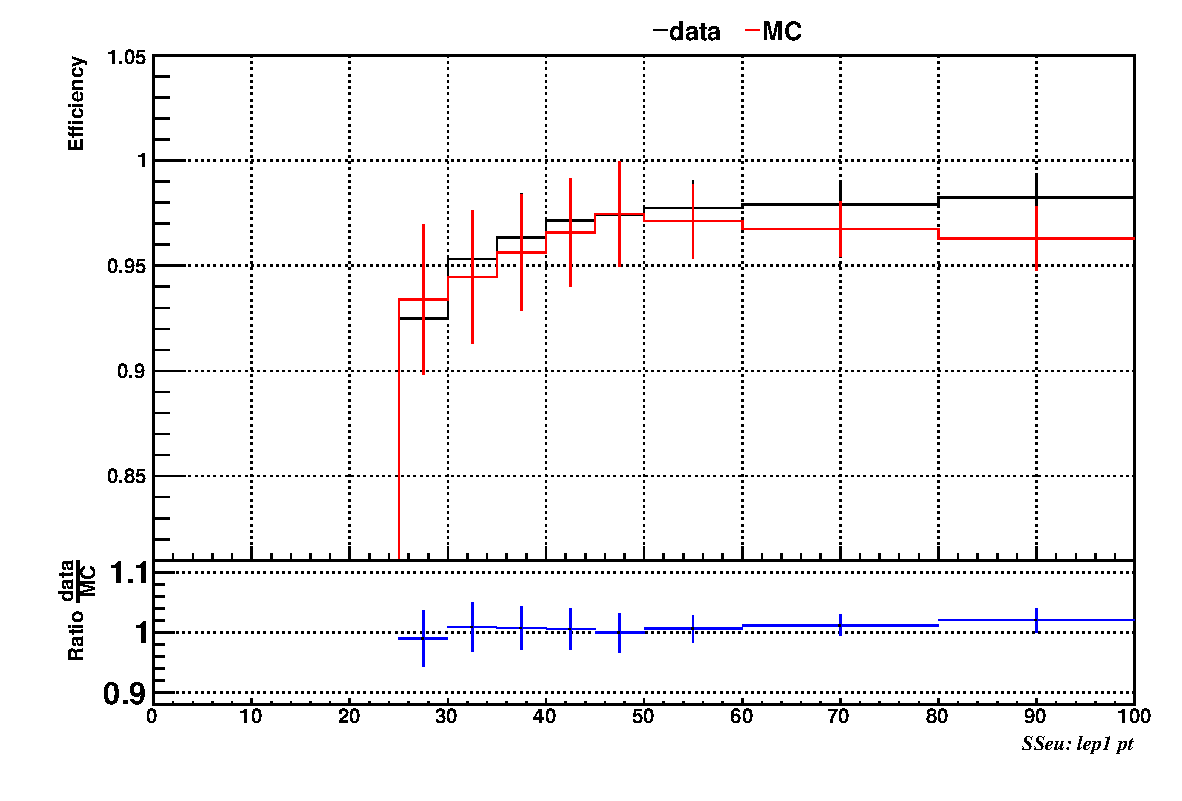
\includegraphics[width=0.49\textwidth]{plots_trigger/1D_eff_lep1_pt_eu_ARCv2_change_3l_pt_ranges.pdf}
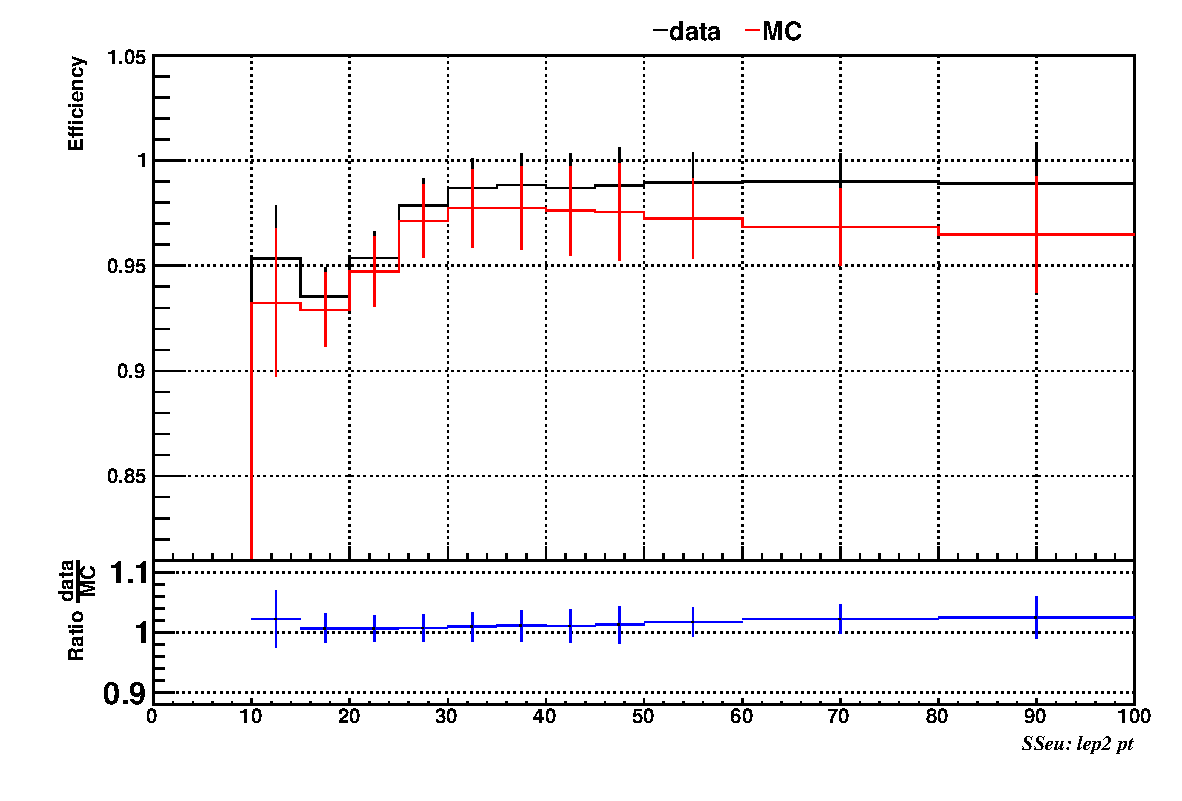
\includegraphics[width=0.49\textwidth]{plots_trigger/1D_eff_lep2_pt_eu_ARCv2_change_3l_pt_ranges.pdf} \\
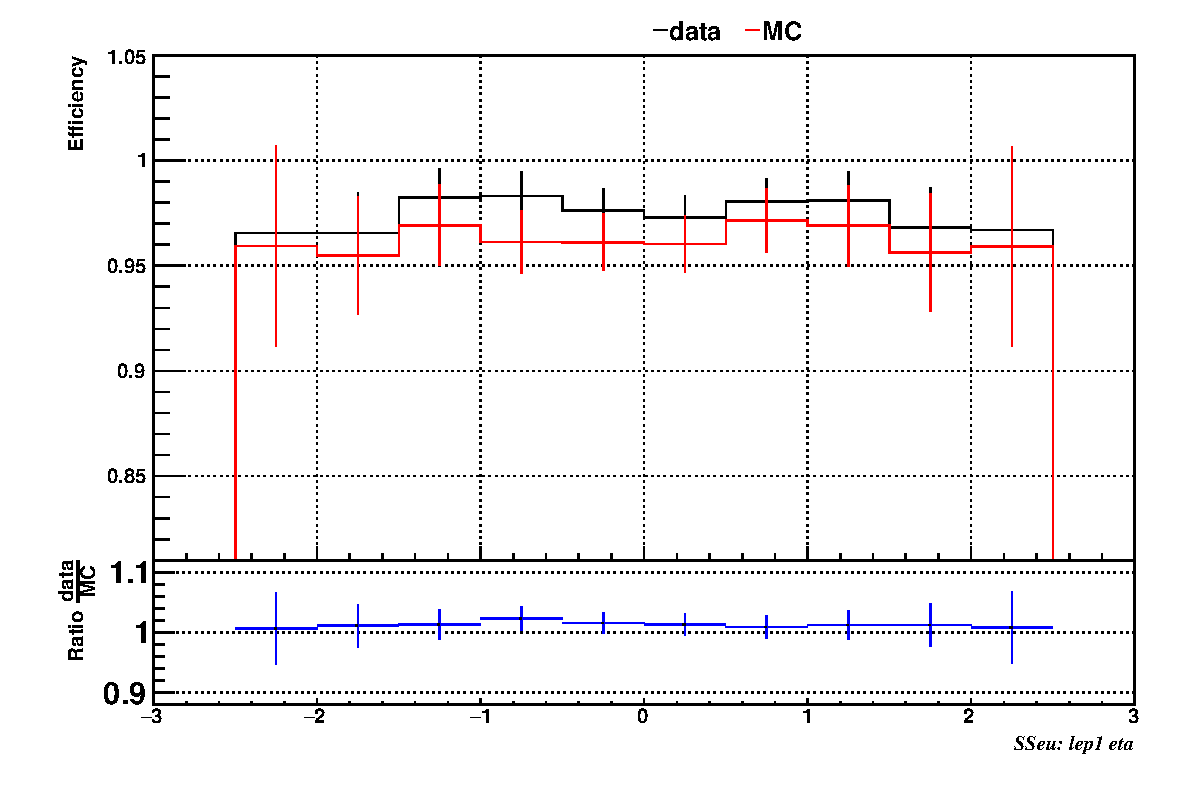
\includegraphics[width=0.49\textwidth]{plots_trigger/1D_eff_lep1_eta_eu_ARCv2_change_3l_pt_ranges.pdf}
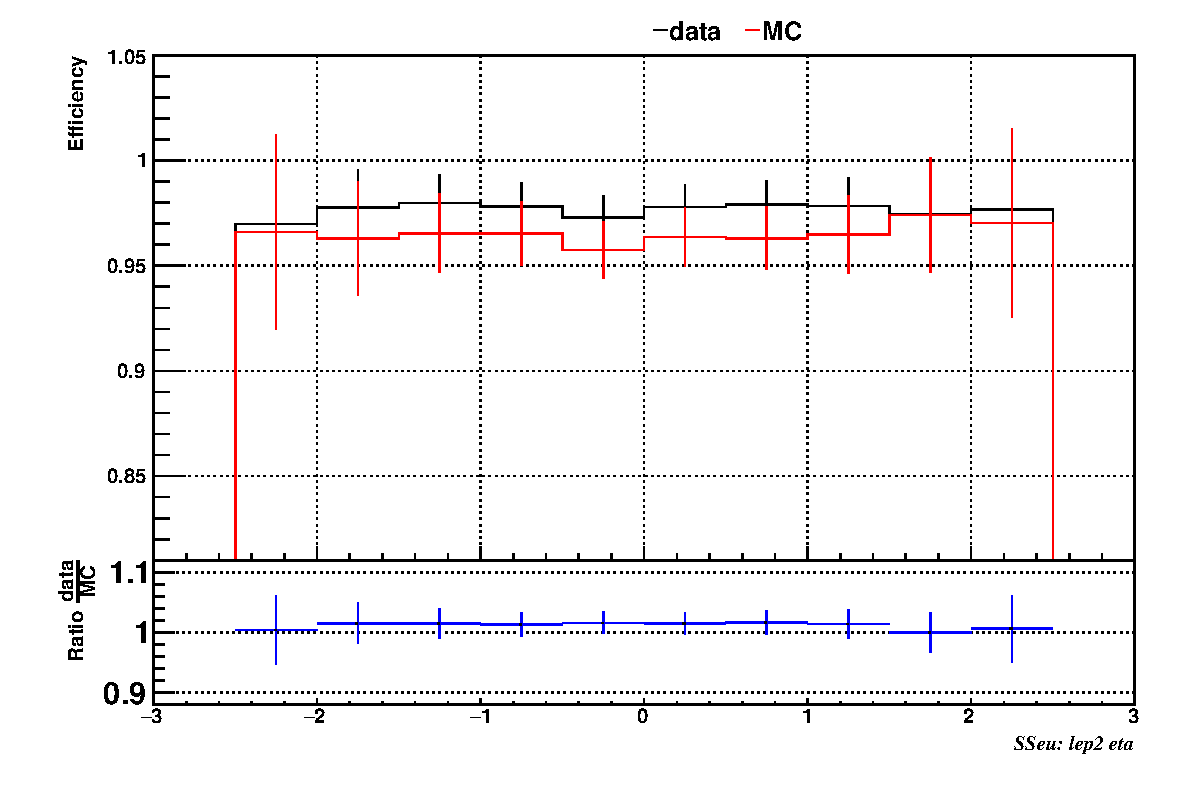
\includegraphics[width=0.49\textwidth]{plots_trigger/1D_eff_lep2_eta_eu_ARCv2_change_3l_pt_ranges.pdf}
\caption{Comparison of the trigger efficiency in the same-sign muon+electron category before 
corrections, shown as a function of the \pt and $\eta$ of the leading lepton (left) 
and the sub-leading lepton (right).}
\label{fig:trigeffsemu}
\end{figure}

\begin{figure}[htp]
\centering
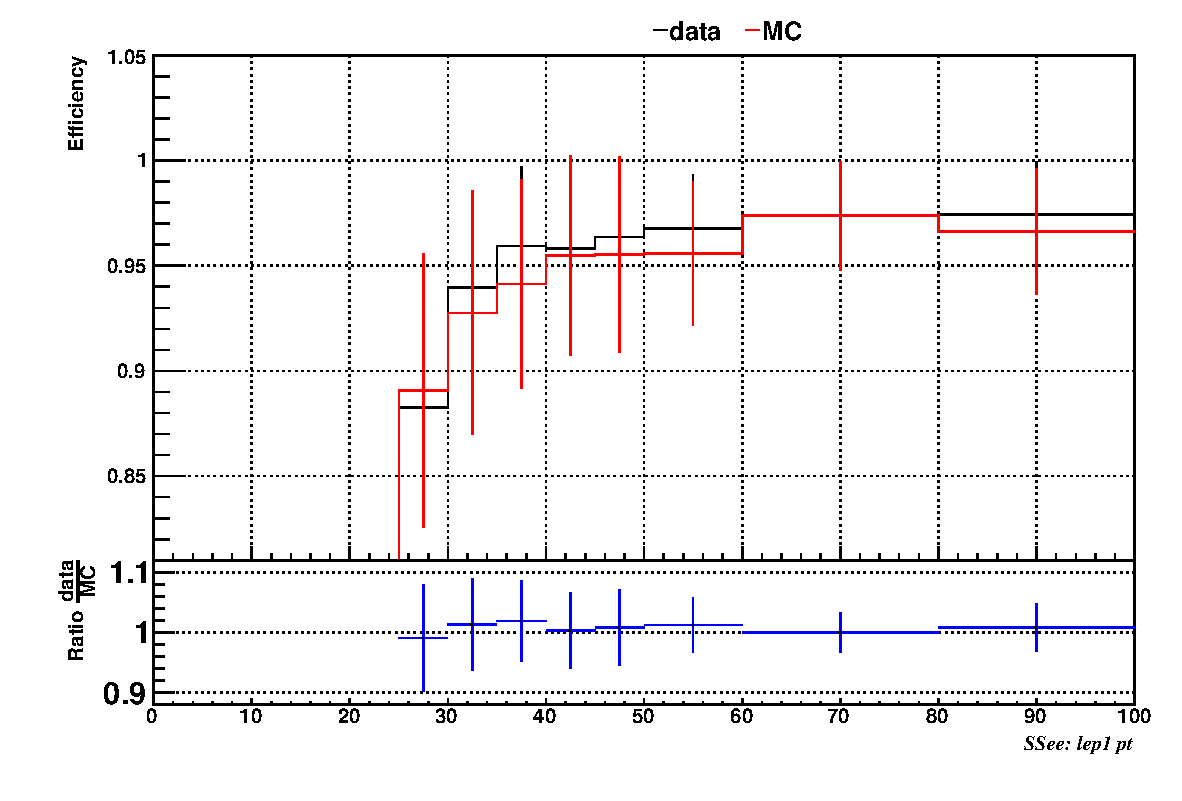
\includegraphics[width=0.49\textwidth]{plots_trigger/1D_eff_lep1_pt_ee_ARCv2_change_3l_pt_ranges.pdf}
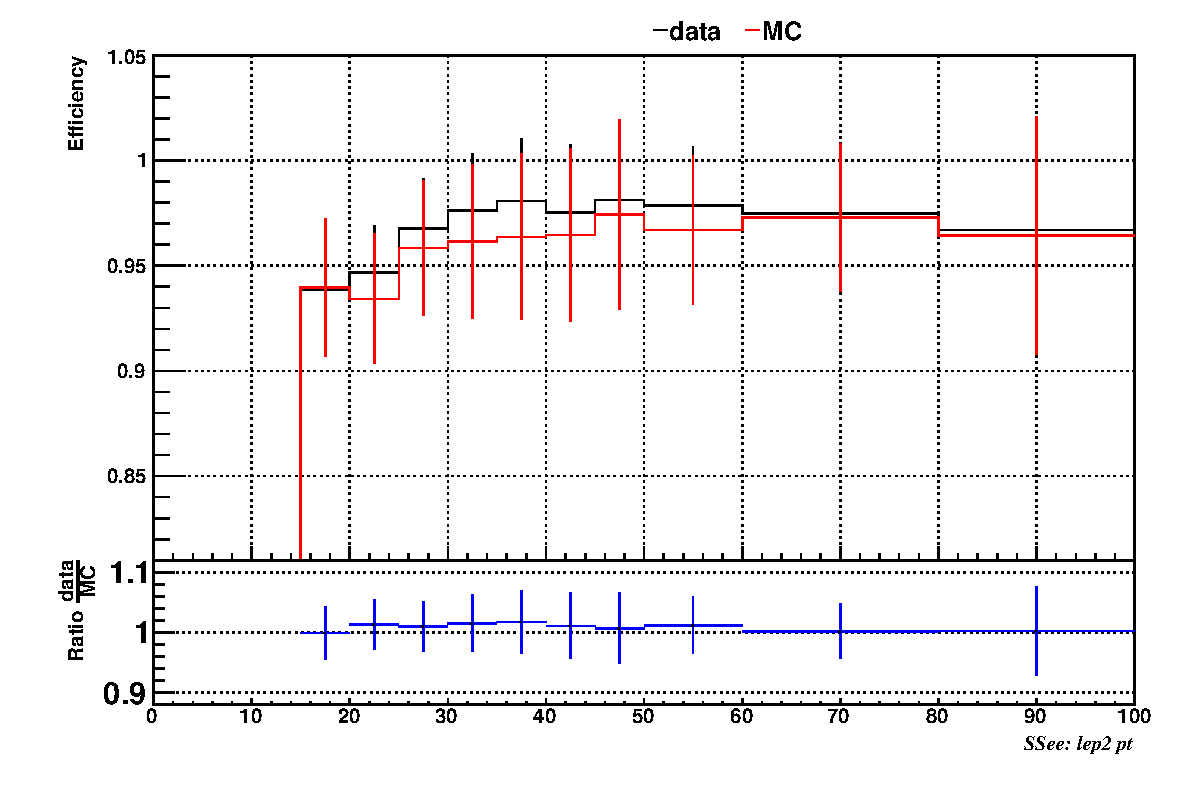
\includegraphics[width=0.49\textwidth]{plots_trigger/1D_eff_lep2_pt_ee_ARCv2_change_3l_pt_ranges.pdf} \\
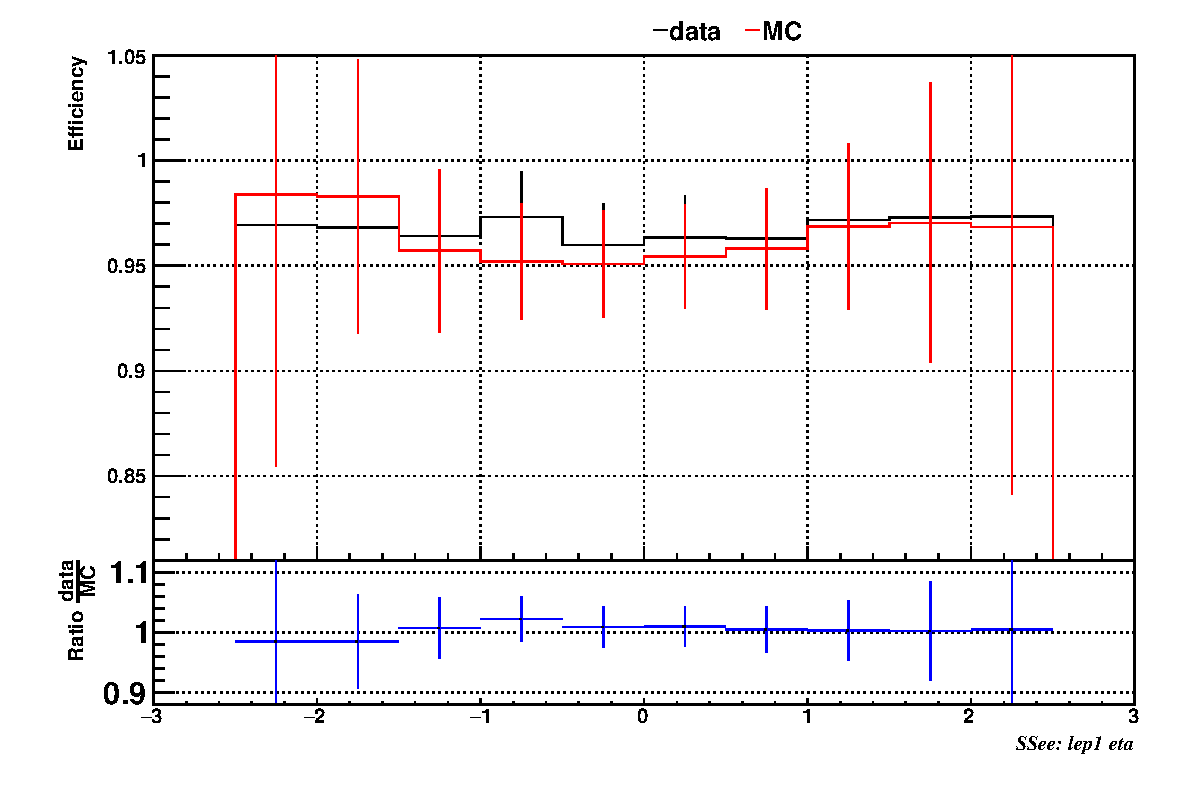
\includegraphics[width=0.49\textwidth]{plots_trigger/1D_eff_lep1_eta_ee_ARCv2_change_3l_pt_ranges.pdf}
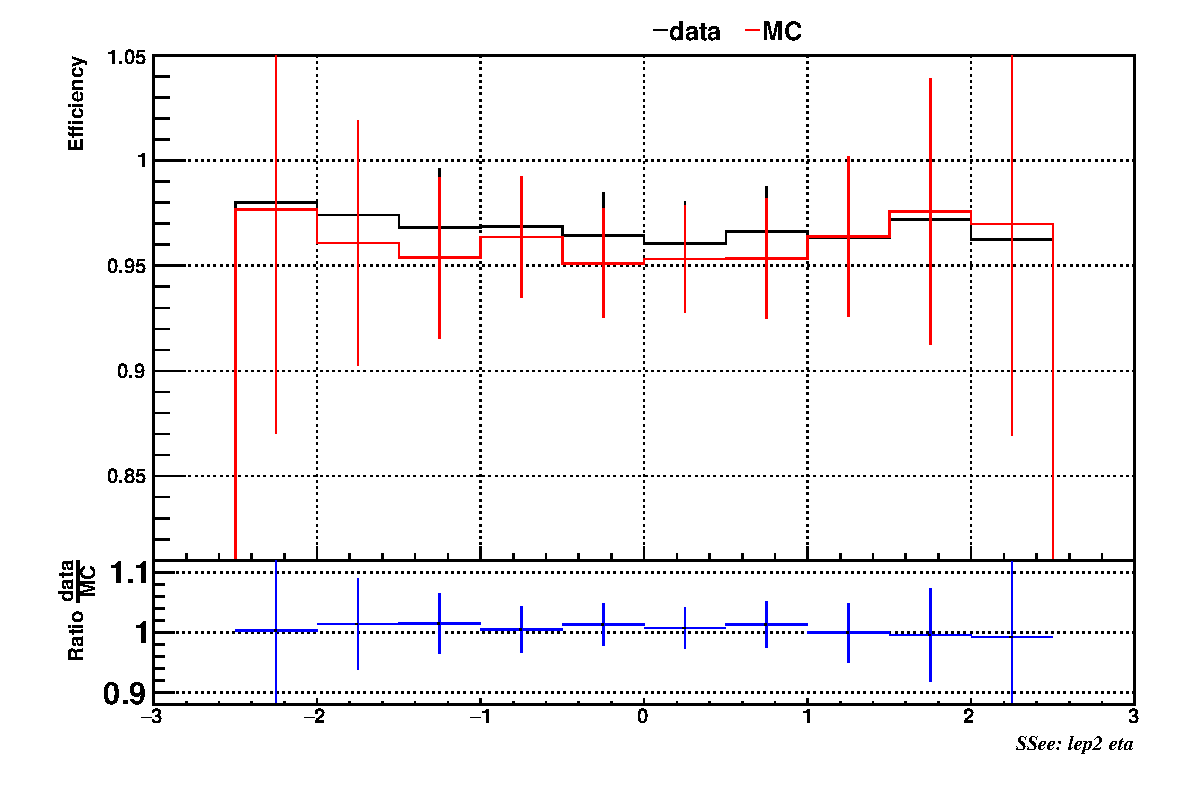
\includegraphics[width=0.49\textwidth]{plots_trigger/1D_eff_lep2_eta_ee_ARCv2_change_3l_pt_ranges.pdf}
\caption{Comparison of the trigger efficiency in the same-sign dielectron category before 
corrections, shown as a function of the \pt and $\eta$ of the leading lepton (left) 
and the sub-leading lepton (right).}
\label{fig:trigeffsee}
\end{figure}

\begin{figure}[htp]
\centering
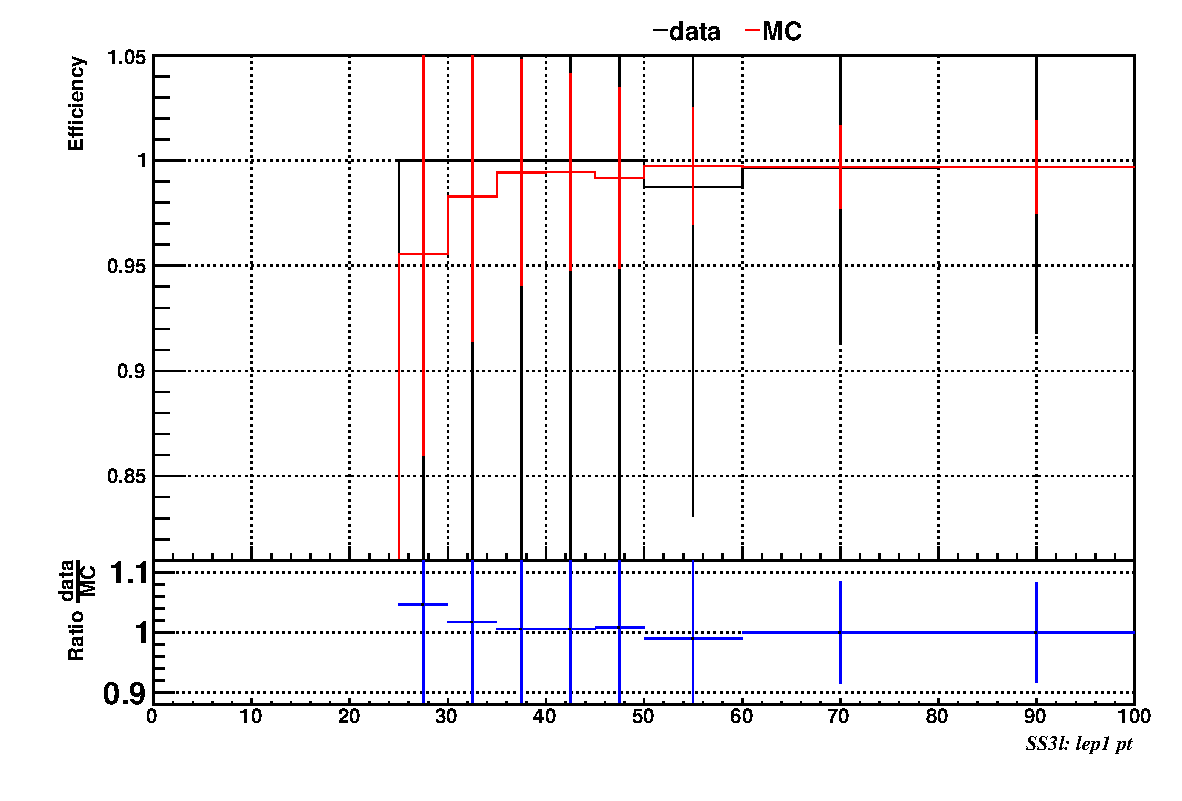
\includegraphics[width=0.49\textwidth]{plots_trigger/1D_eff_lep1_pt_3l_ARCv2_change_3l_pt_ranges.pdf}
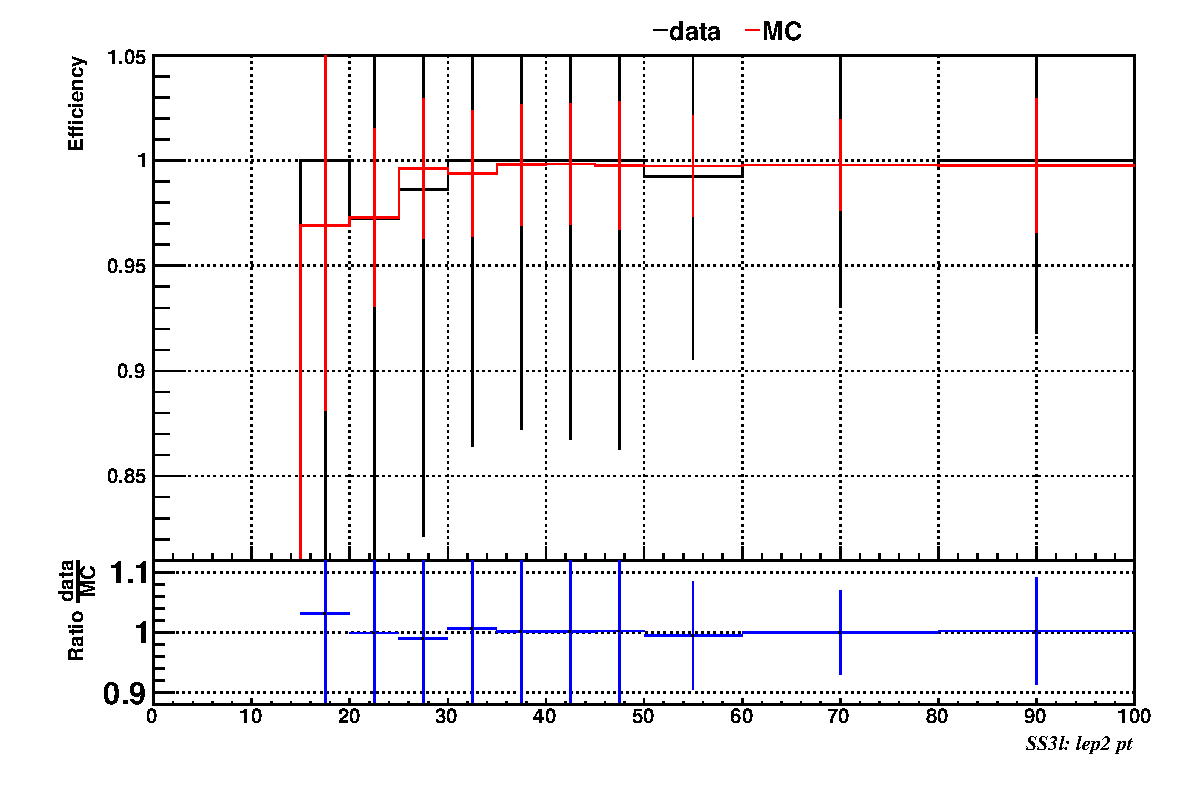
\includegraphics[width=0.49\textwidth]{plots_trigger/1D_eff_lep2_pt_3l_ARCv2_change_3l_pt_ranges.pdf} \\
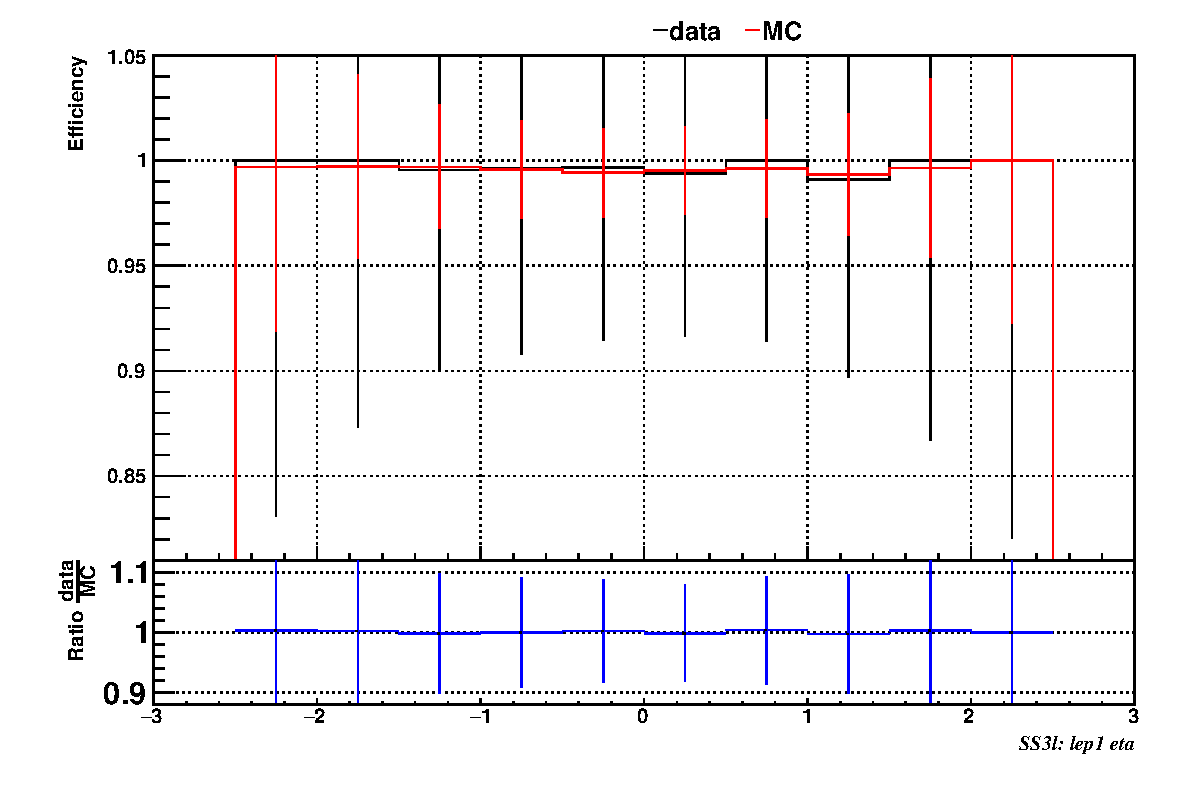
\includegraphics[width=0.49\textwidth]{plots_trigger/1D_eff_lep1_eta_3l_ARCv2_change_3l_pt_ranges.pdf}
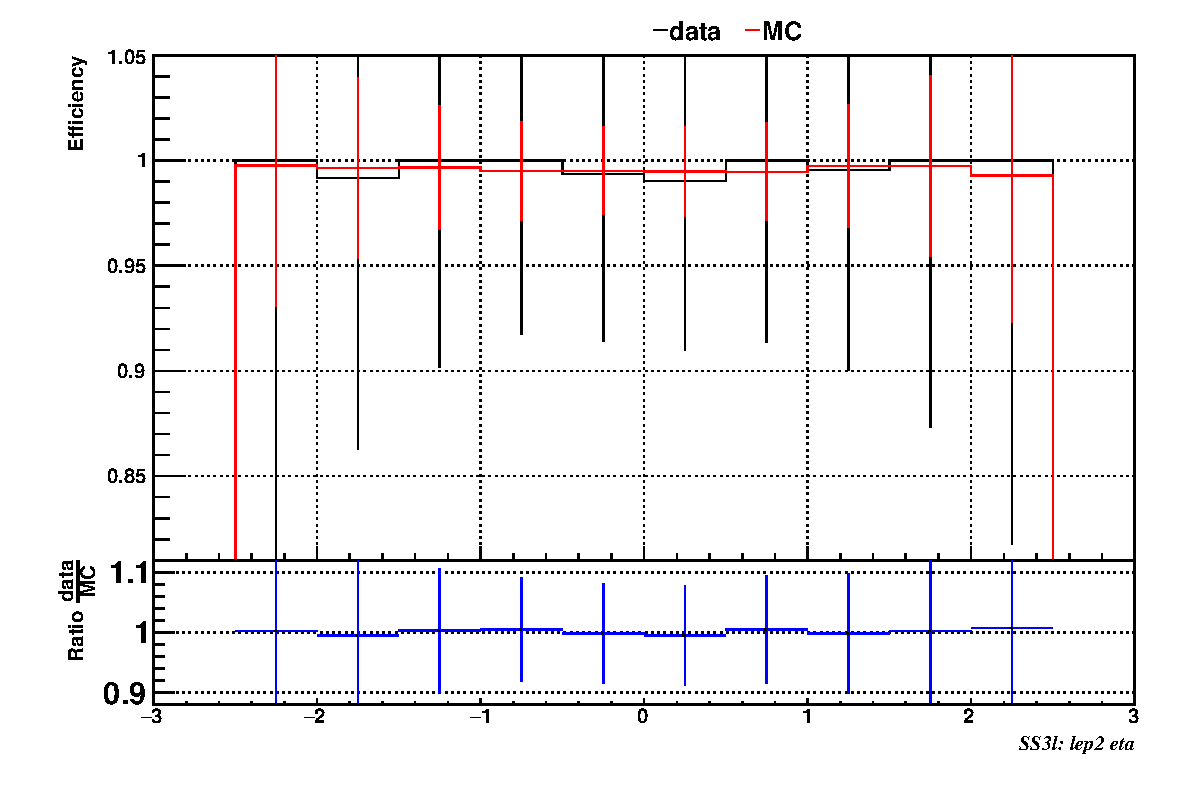
\includegraphics[width=0.49\textwidth]{plots_trigger/1D_eff_lep2_eta_3l_ARCv2_change_3l_pt_ranges.pdf}
\caption{Comparison of the trigger efficiency in the $\geq 3$-lepton category before 
corrections, shown as a function of the \pt and $\eta$ of the leading lepton (left) 
and the sub-leading lepton (right).}
\label{fig:trigeffs3l}
\end{figure}

%\begin{figure}[htp]
%\centering
%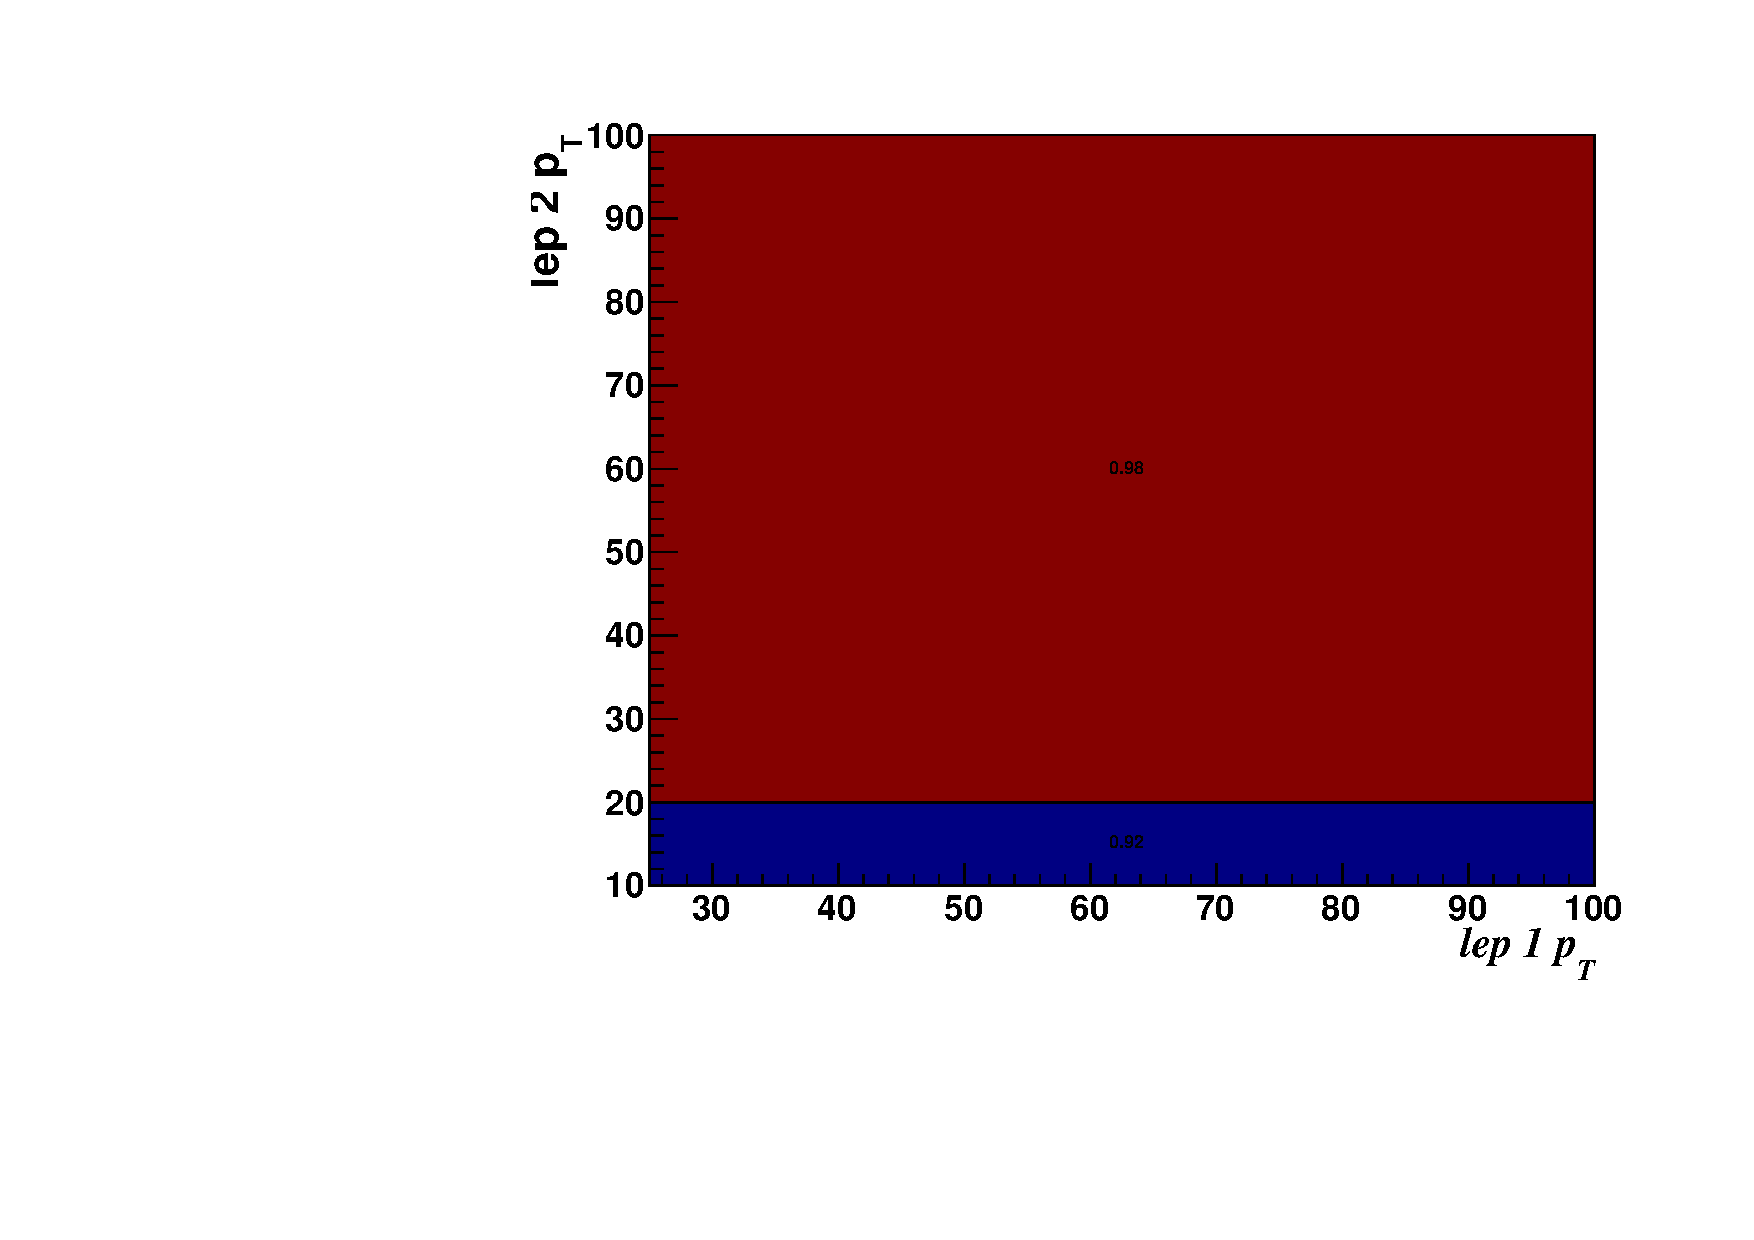
\includegraphics[width=0.49\textwidth]{plots_trigger/trigEffRegions_uu_v2.pdf}
%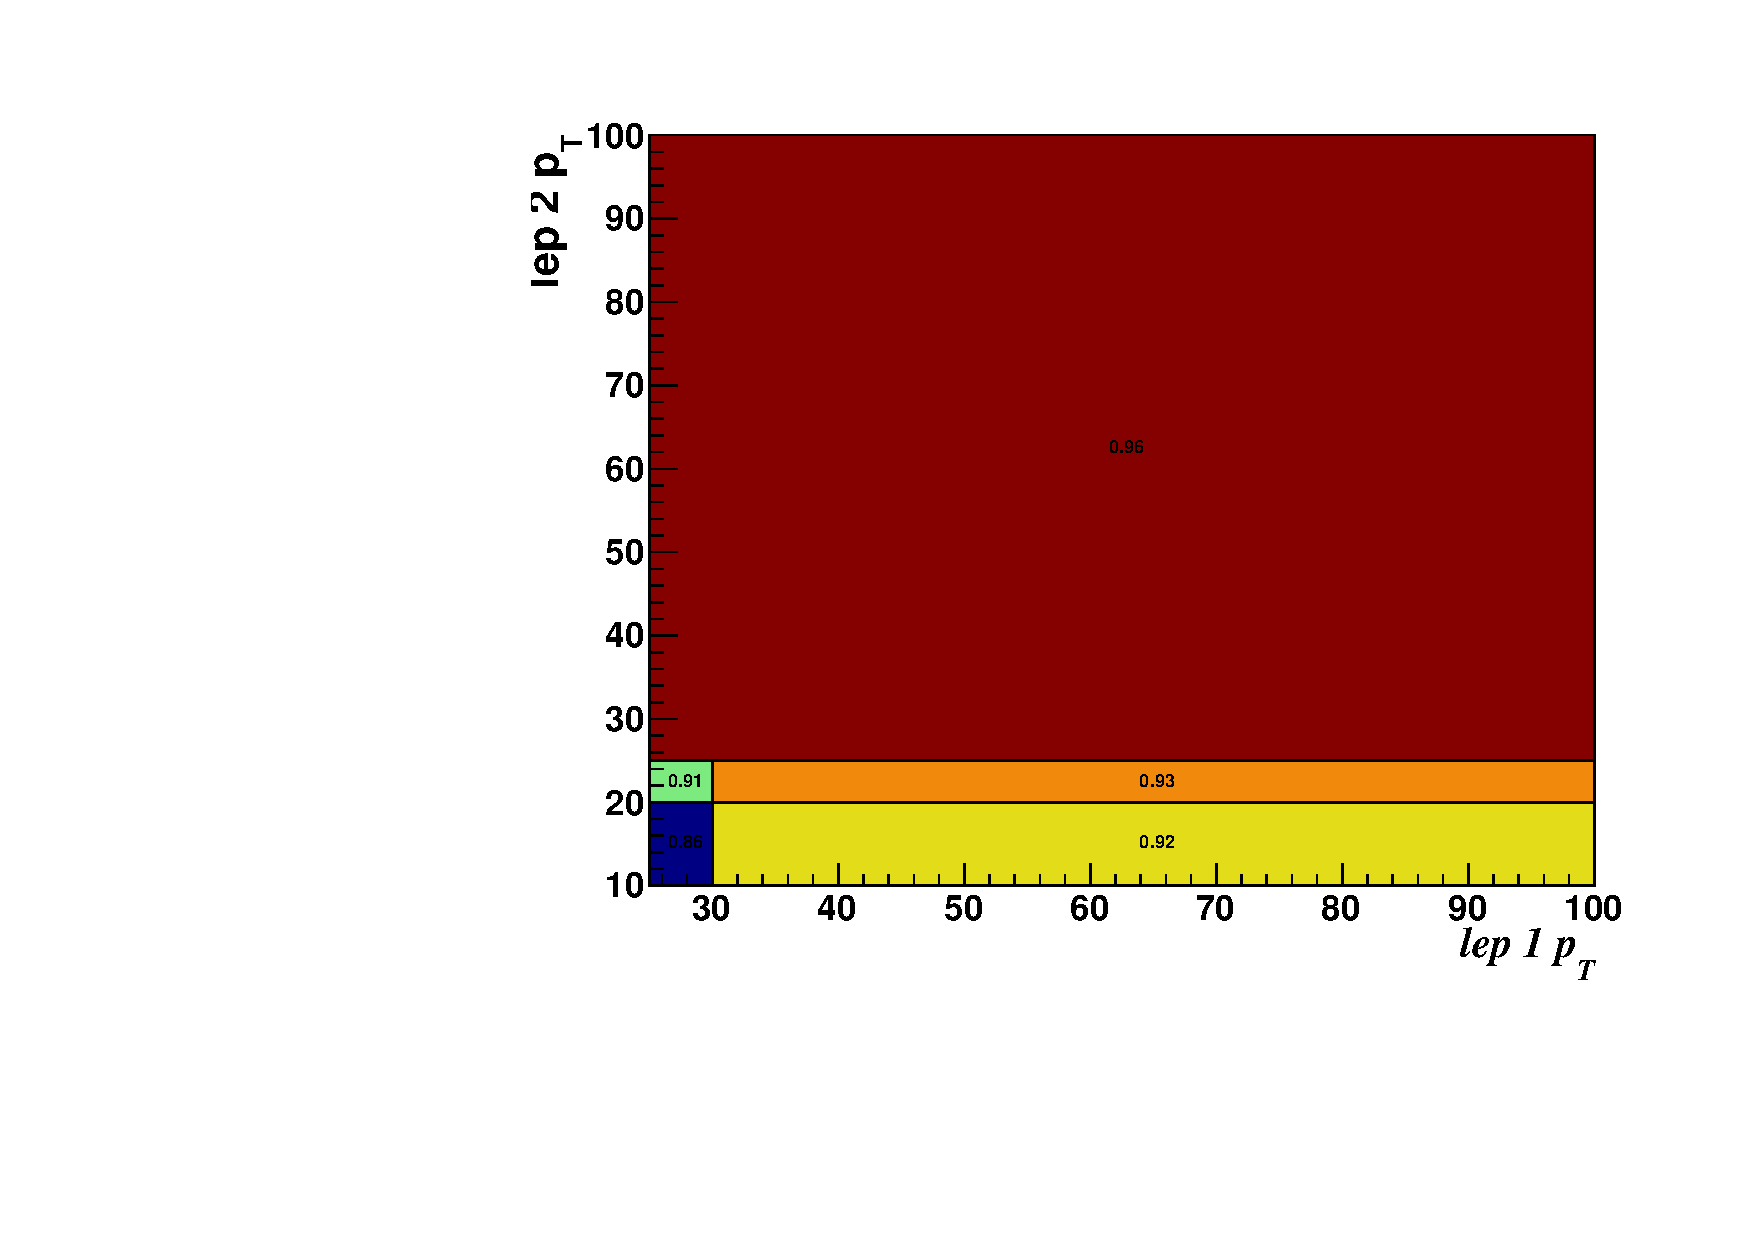
\includegraphics[width=0.49\textwidth]{plots_trigger/trigEffRegions_eu_v2.pdf} \\
%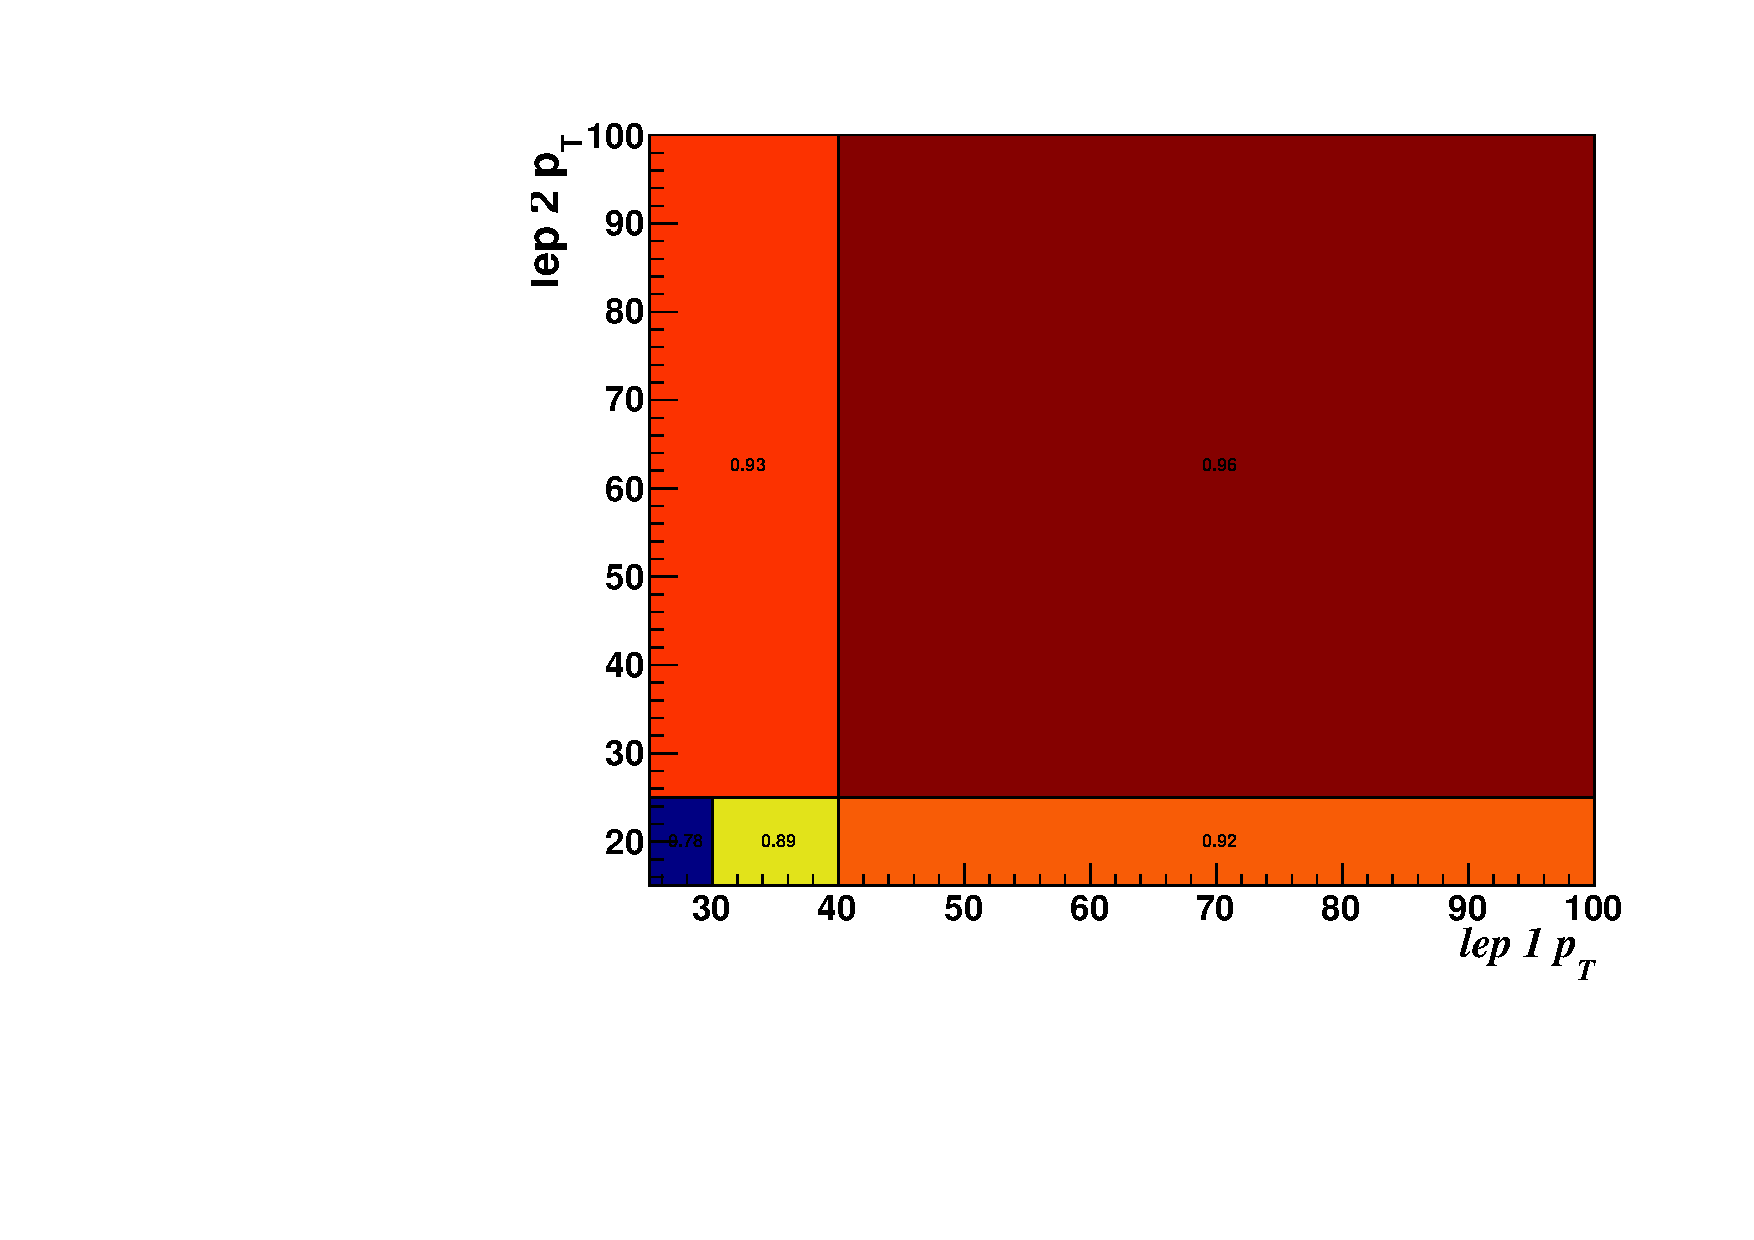
\includegraphics[width=0.49\textwidth]{plots_trigger/trigEffRegions_2e_v2.pdf}
%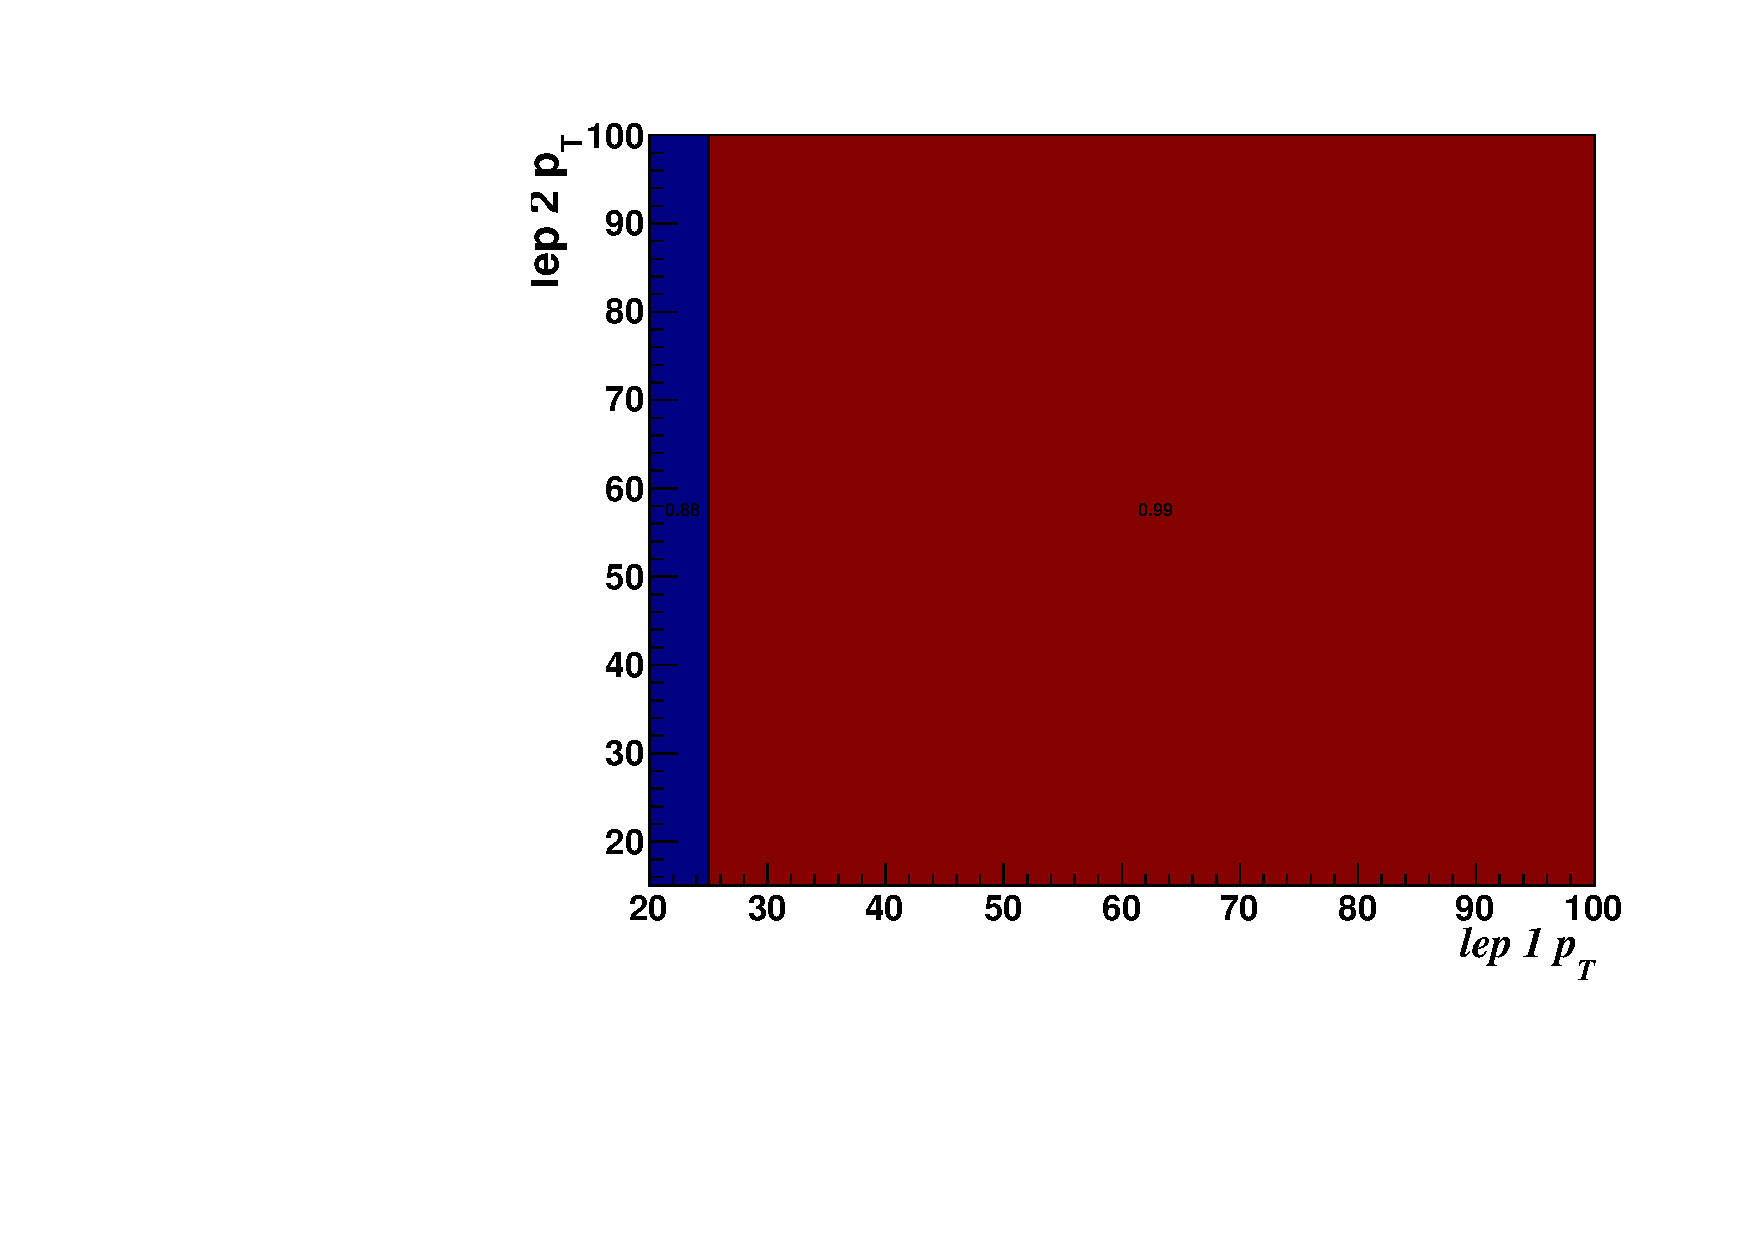
\includegraphics[width=0.49\textwidth]{plots_trigger/trigEffRegions_3l_v2.pdf}
%\caption{Clockwise from top left: trigger efficiency regions in the same-sign dimuon, 
%same-sign muon+electron, 3 lepton and same-sign dielectron categories.}
%\label{fig:trigeffsWeights}
%\end{figure}

%\begin{figure}[htp]
%\centering
%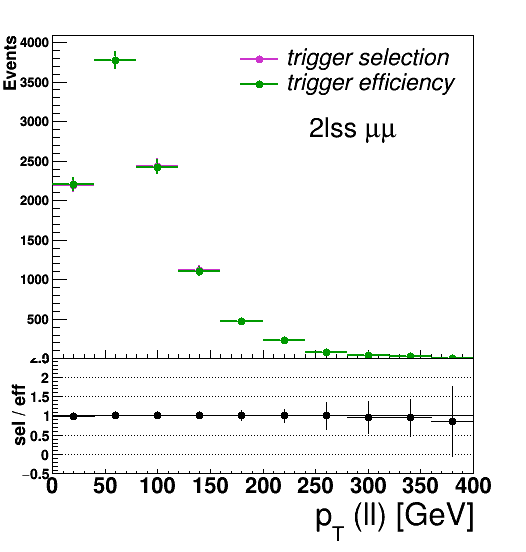
\includegraphics[width=0.32\textwidth]{plots_trigger/dilep_pt_2lss_mm_trg_closure.png}
%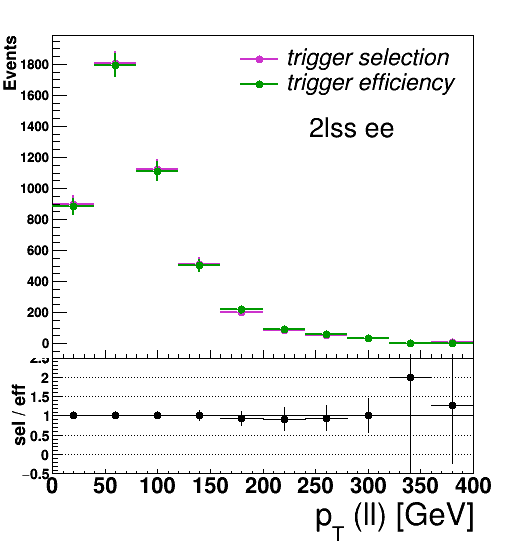
\includegraphics[width=0.32\textwidth]{plots_trigger/dilep_pt_2lss_ee_trg_closure.png}
%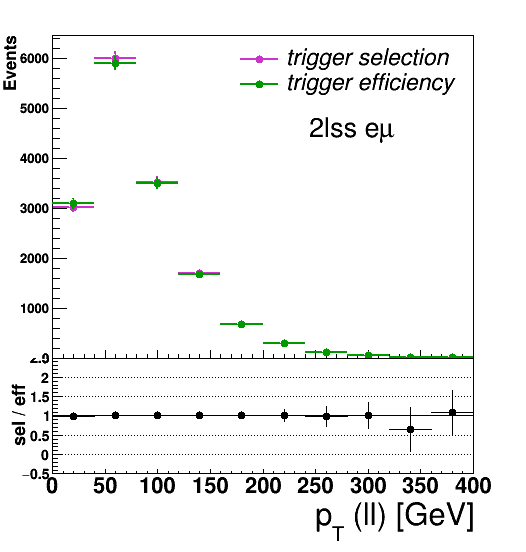
\includegraphics[width=0.32\textwidth]{plots_trigger/dilep_pt_2lss_em_trg_closure.png}\\
%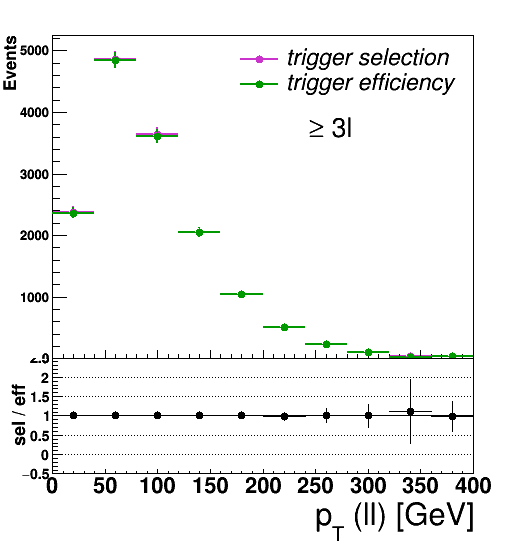
\includegraphics[width=0.32\textwidth]{plots_trigger/dilep_pt_3l_trg_closure.png}
%\caption{Closure test showing the difference between applying the trigger selection directly to ttH MC
%and applying the derived trigger efficiency to ttH MC. Here, the dilepton \pt distribution
%in the 2$\ell$ ($\Pgm\Pgm$, $\Pe\Pe$, $\Pe\Pgm$) categories (top), and the 3$\ell$ category (bottom) is shown.
%Uncertainties are statistical only.}
%\label{fig:trigClosure}
%\end{figure}


\begin{table}
\footnotesize
\centering
\begin{tabular}{l | l}
\hline
Category & Scale Factor \\
\hline
2e & $1.01 \pm 0.02$ \\
e+mu & $1.01 \pm 0.01$ \\
2mu & $1.00 \pm 0.01$ \\
3 and 4l & $1.00 \pm 0.03$ \\
\hline
\end{tabular}
\caption{Trigger efficiency scale factors and associated uncertainties, shown here rounded to the nearest percent.}
\label{tab:trigSFs}
\end{table}

\clearpage


\section{Event reconstruction and object identification}
\label{sec:objects}
A complete reconstruction of the individual particles from
each collision event is obtained via the particle-flow (PF) algorithm.
The technique uses the information from all CMS sub-detectors to identify and
reconstruct individual particles in the collision
event~\cite{CMS-PAS-PFT-09-001, CMS-PAS-PFT-10-002}. The particles are
classified into mutually exclusive categories: charged hadrons,
neutral hadrons, photons, muons, and electrons.

\subsection{Jets and B-tagging}
Jets are reconstructed by clustering PF candidates using the
anti-$\mathrm{k_T}$ algorithm with distance parameter $\Delta
\mathrm{R}=0.4$ as implemented in the \textsc{fastjet} package~\cite{Cacciari:fastjet1,Cacciari:fastjet2}. 
The charged hadrons not coming from the primary vertices are subtracted from the
PF candidates considered in the clustering. The primary vertex is
chosen as the vertex with the highest sum of $\PT^2$ of its
constituent tracks. The prescribed jet energy corrections are applied as a function
of the jet $E_T$ and $\eta$~\cite{cmsJEC}. In addition, a multivariate
discriminator is applied to distinguish between jets coming from the
primary vertex and jets coming from pile-up vertices.  The
discrimination is based on the differences in the jet shapes, in the
relative multiplicity of charged and neutral components, and in the
different fraction of transverse momentum which is carried by the
hardest components.  Within the tracker acceptance the jet tracks are
also required to be compatible with the primary vertex. Jets are only
considered if they have a transverse energy above $25 \GeV$ and
$|\eta|<$2.4. In addition, they have to be separated from any lepton
candidates passing the Fakeable Object selection, described below, by requiring $\Delta \mathrm{R} = \sqrt{(\eta^{\ell} -
\eta^{jet})^{2} + (\phi^{\ell} - \phi^{jet})^{2}}>0.4$.

The CSVv2 b-tagging algorithm~\cite{Chatrchyan:2012jua} is used to
identify jets that are likely to originate from the hadronization of bottom
quarks.  This algorithm combines both secondary vertex information and
track impact parameter information together in a likelihood
discriminant. The discriminant output value ranges from
zero to one. It distinguishes between $b$-jets and jets
originating from light quarks, gluons and charm quarks.  The
efficiency to tag $b$-jets and the rate of misidentification of non-b
jets depend on the operating point chosen. Both the efficiency
and the fake rate are parameterised as a function of the transverse momentum and
pseudorapidity of the jets. These performance measurements are
obtained directly from data in samples that can be enriched in b jets,
such as $\ttbar$ and multijet events where a muon can be found inside the one of jets.
Two working points for the CSVv2 output discriminant  are used in the analysis. The
\emph{loose} one (CSVv2 $>$ 0.5426) has approximately ${85}$\% efficiency to tag jets
with $b$ quarks and a ${10}$\% chance to tag jets with only light quarks
or gluons.  The \emph{medium} working point (CSVv2 $>$ 0.8484) has
approximately ${70}$\% efficiency for tagging jets with $b$ quarks
and ${1.5}$\% efficiency to tag jets with only light quarks or gluons
~\cite{Chatrchyan:2012jua}.\\

%We correct for data/sim differences in the b-tagging performance by
%applying to the simulation per-jet weights dependent on the jet pt,
%eta, b-tagging discriminator and flavour (from simulation truth). 
%The weights are derived on ttbar and Z+jets events. 
%The per-event weight is taken as the product of the per-jet weight, 
%including those of the jets associated to the leptons.\\


\subsection{Missing Energy}
The missing transverse energy vector is calculated offline as the
negative of the vector sum of transverse momenta of all PF candidates
identified in the event. The magnitude of this vector is referred to
as $E_{T}^{miss}$. To recover from the 
performance degradation of the missing transverse energy due to pile-up
interactions, we also consider the $H_{T}^{miss}$ variable, computed in
the same way as the $E_{T}^{miss}$, but using only the
selected jets and leptons (the lepton selection will be described in
the following paragraphs).  The $H_{T}^{miss}$ variable has worse
resolution than $E_{T}^{miss}$ but is more robust as it does
not rely on the soft part of the event.  In this analysis the event
selection makes use of a linear discriminator based on the two
variables, $E_{T}^{miss}LD$, exploiting the fact that $E_{T}^{miss}$
and $H_{T}^{miss}$ are less correlated in events with instrumental
missing energy with respect to events with real missing energy.
The $E_{T}^{miss}LD$ is defined as
\begin{equation}
 E_{T}^{miss}LD= E_{T}^{miss}*0.00397 + H_{T}^{miss}*0.00265
\label{eq:reconstruction_isolation}
\end{equation}
and the working point used is
$E_{T}^{miss}LD>0.2$, as in HIG-15-008.
%%%Fig.\,\ref{fig:met} shows the correlation
%%%between $H_{T}^{miss}$ and $E_{T}^{miss}$ in signal events and
%%%DY+jets events and the comparison between the performances of the two
%%%variables and the linear discriminator.


%%%\begin{figure}[htb]
%%%\centering
%%%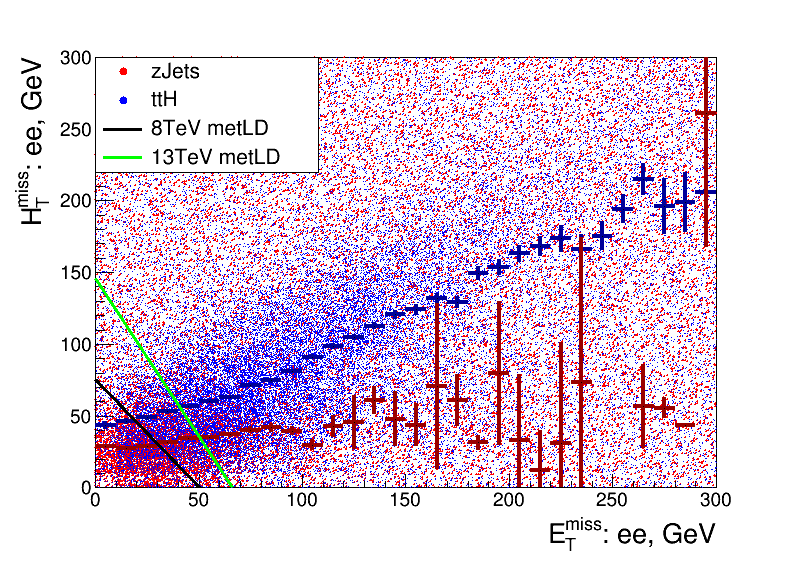
\includegraphics[width=0.50\linewidth]{plots_met/2Dplot_metld_ee.png} 
%%%\caption{The figure shows the correlation between the
%%%$H_{T}^{miss}$ and $E_{T}^{miss}$ variables in signal events (blue) and
%%%DY+jets events (red). This analysis uses the 
%%%\emph{8 TeV met LD} cut.} 
%%%\label{fig:met}
%%%\end{figure}

\subsection{Lepton Identification}
In this analysis, \emph{background leptons} are defined as leptons
coming from b-hadron decays, the misidentification of
light jets, and photon conversions. We define \emph{signal leptons}
as the isolated leptons coming from W, Z, and $\tau$ decays.\\
The reconstruction and identification of electron
and muon candidates is described first, followed by the advanced identification criteria
used to retain the highest possible efficiency for signal leptons
while rejecting background leptons.


\subsubsection{Muons reconstruction and identification}
Muon candidates are reconstructed combining the information from both the silicon tracker and the
muon spectrometer in a global fit~\cite{Chatrchyan:2012xi}. An identification selection is
performed using the quality of the geometrical matching between the
tracker and the muon system measurements.\\
Two working points are considered for the muon identification. The
loose working point, "POG Loose ID" described in
\cite{MuId}, and a tighter working point given by the list of
requirements on the muon segment-compatibility variable, known as the "POG Medium Id", defined in
\cite{muonMediumId}. The usage of each working point will be described
in Table~\ref{tab:muonIDs}. Only muons within the muon system acceptance
$|\eta|<2.4$ and minimum $\pt$ cuts of 5~GeV are considered.\\


\subsubsection{Electron reconstruction and identification}
Electrons are reconstructed using tracking and electromagnetic
calorimeter information by combining ECAL superclusters and gaussian
sum filter (GSF) tracks.
We require electrons to have $|\eta| < 2.5$ to
ensure that they are within the tracking volume and a minimum $\pt$ of
7~GeV. \\
The electron identification is performed using a multivariate
discriminant built with shower-shape variables ($\sigma_{i\eta
  i\eta}$, $\sigma_{i\phi i\phi}$, the cluster circularity, widths
along $\eta$ and $\phi$, $\mbox{R}_9$, H/E,
$\mbox{E}_{inES}/\mbox{E}_{raw}$), track-cluster matching variables
($E_{tot}/p_{in}$, $E_{Ele}/p_{out}$, $\Delta\eta_{in}$,
$\Delta\eta_{out}$, $\Delta\phi_{in}$, $1/E-1/p$  ) and track quality
variables ($\chi^2$ of the KF and GSF tracks, the number of hits used
by the KF/GSF filters, fbrem). A complete description of the
multivariate discriminant (MVA ID) and training used can be found in
\cite{elMvaIdBase}. A loose selection based on eta-dependent cuts on
this discriminant is used to preselect our electron candidates, the full shape
of the discriminant is used in the lepton multivariate selection to
separate signal leptons from background leptons. Additional
identification criteria are applied for electrons with $\pt$ greater
than 30 GeV to mimic the identification applied at trigger level in order to
ensure consistency between the \emph{measurement} region and \emph{application}
region of the fake-rate (as it will be described in dedicated sections).\\
All the selection criteria will be described in Table~\ref{tab:eleIDs}.


\subsubsection{Lepton vertexing}
With the goal of rejecting pile-up or mis-reconstructed tracks,
and more importantly to reject background leptons from b-hadron decays,
the following impact parameter variables are also considered: impact parameter in
the transverse plane $d_0$, impact parameter along the $z$ axis $d_z$,
and the impact parameter significance in the detector space $\text{SIP}_{3D}$.\\
Loose cuts are applied on this variables to achieve the first goal,
while the full shape of the same variables is used in a multivariate
approach to reach the best separation between the signal and the
background leptons. \\
The details of the selections are provided in Table~\ref{tab:muonIDs} and Table~\ref{tab:eleIDs}.


\subsubsection{Lepton isolation}
The charged leptons produced in decays of heavy particles, such as $\PW$ and $\cPZ$ bosons,
are typically spatially isolated from the hadronic activity in the event,
while the leptons produced in the decays of hadrons or misidentified leptons are usually
embedded in jets. This distinction becomes less evident moving to
highly boosted systems where decay products tend to overlap.
Therefore, given the higher collision energy, instead of using the
standard PF Isolation where all the neutral, charged hadrons and
photons are considered in a cone of $\Delta R = \sqrt{(\eta^\ell - \eta^i)^{2} + (\phi^\ell- \phi^i)^{2}} < 0.3$
around the leptons, a new isolation variable is constructed: the mini isolation \miniIso. \\
Requiring \miniIso below a given threshold ensures that the lepton is locally isolated, even in boosted topologies. The impact of pileup is mitigated using the so-called effective area correction:
  \begin{equation}
    \miniIso = \frac{\sum_R \pt(h^\pm) - \mbox{max}(0, \sum_R \pt(h^0)+\pt(\gamma) - \rho\mathcal{A}\left(\frac{R}{0.3}\right)^2}{\pt(\ell)}.
  \end{equation}
where $\rho$ is the pileup energy density, while $\sum_R\pt(h^\pm)$, $\sum_R\pt(h^0)$ and $\sum_R\pt(\gamma)$ refers to the sum of the transverse momentum of the charged hadrons, neutral hadrons and photons, respectively, within a cone $R$, dependent of the lepton \pt:
\begin{equation}
  R = \frac{10}{\mbox{min}(\mbox{max}(\pt(\ell), 50), 200)}
\end{equation}
The effective areas $\mathcal{A}$ used are listed in Table \ref{tab:EffArea}.
\begin{table}[h]
  \begin{center}
    \small
    \begin{tabular}{|l||c|c|}
      \hline
      $|\eta|$ range & $\mathcal{A}$(e) neutral/charged &  $\mathcal{A}$($\mu$) neutral/charged \\
      \hline\hline
      $0.0-0.8$ & 0.1607 / 0.0188 & 0.1322 / 0.0191 \\
      $0.8-1.3$ & 0.1579 / 0.0188 & 0.1137 / 0.0170 \\
      $1.3-2.0$ & 0.1120 / 0.0135 & 0.0883 / 0.0146 \\
      $2.0-2.2$ & 0.1228 / 0.0135 & 0.0865 / 0.0111 \\
      $2.2-2.5$ & 0.2156 / 0.0105 & 0.1214 / 0.0091 \\
      \hline
    \end{tabular}
    \caption{Effective areas, for muons and electrons}
    \label{tab:EffArea}
  \end{center}
\end{table}
A very loose cut on this variable is applied to pre-select the muon
and electron candidates, while the full shape is used in the
multivariate discriminator for the signal lepton selection.
Again, details of the selections are provided in Table~\ref{tab:muonIDs} and Table~\ref{tab:eleIDs}.

\subsubsection{Jet-related variables}
In this analysis the most important source of misidentified leptons
comes from the decay of b-hadrons (from $\ttbar$+jets , DY+jets, and
$\PW$+jets events). We therefore want to use in addition to the
vertexing and isolation variables described above additional handles
to target the rejection of this particular type of background leptons.
These additional variables are related to the jet reconstructed in the event closest to
the lepton. In particular we use the
 PF jets reconstructed around the leptons, requiring $\Delta \mathrm{R} =
\sqrt{(\eta^{\ell} - \eta^{jet})^{2} + (\phi^{\ell} -
\phi^{jet})^{2}}<0.5$; charged hadrons from pile-up primary vertices
are not removed prior to the jet clustering. The four considered
variables are the ratio between the $\pt$ of the
lepton and the $\pt$ of the jet, the CSV b-tagging discriminator value of
the jet, the number of charged tracks of the jet, and the \ptRel variable:
  \begin{equation}
    \ptRel=\frac{(\vec{p}(\mbox{jet})-\vec{p}(\ell))\cdot \vec{p}(\ell) }{||\vec{p}(\mbox{jet})-\vec{p}(\ell)||}.
  \end{equation}

In order to avoid an over-correction on prompt leptons, the
application of the jet energy correction is only applied on the
hadronic part of the jet, using the following formula $\mbox{jet}
= \ell + (\text{jet-PU-}\ell)*JEC - PU$, where $\ell$ is the lepton,
$PU$ the pileup energy clustered into the jet, and $JEC$ the jet
energy scale correction to be applied to any jet.


\subsubsection{Lepton MVA discriminator}
In order to profit from all these handles together, we first
preselect our leptons candidates with the \emph{Loose} selection that will be
described in the following, and we then use a multivariate
discriminator based on boosted decision tree (BDT) techniques to
distinguish signal leptons (from W, Z, or $\tau$
decays) from background leptons (mostly from b-hadron
decays). We refer to it as the {\it lepton MVA discriminator} throughout this
document.  The multivariate discriminator is trained using simulated
signal Loose leptons from the  $t\bar{t}H$ MC sample and fake leptons from the
 $t\bar{t}$+jets MC sample, separately for muons
and electrons. The training used in this analysis is unchanged with respect
to the 2015 analysis, detailed in \cite{CMS_AN_2015-321}. It uses as input variables the vertexing,
isolation and jet-related variables described so far, the $\pt$ and
$\eta$ of the lepton and two additional variables that contribute
to make it robust also in the rejection of leptons from light jets
mis-identification: the electron MVA ID discriminator and the
muon segment-compatibility variables. \\
%In Fig.~\ref{fig:rocsMVA} the performances of the lepton MVA are
%described comparing the efficiency on signal lepton from $t\bar{t}H$
%to the one on background leptons from $t\bar{t}$ that pass the
%preselection. The performances are compared with what we would
%obtained simply using the \miniIso, and with the identification
%working point choose by the same-sign dilepton SUSY analysis
%(SUS-15-008), which is a cut based algorithm based
%on \miniIso, \ptRatio, \ptRel, $\text{SIP}_{3D}$ on top of the Muon Medium ID and a
%tight working point for the electron MVA ID.\\


%\begin{figure}[!htb]
%\centering
%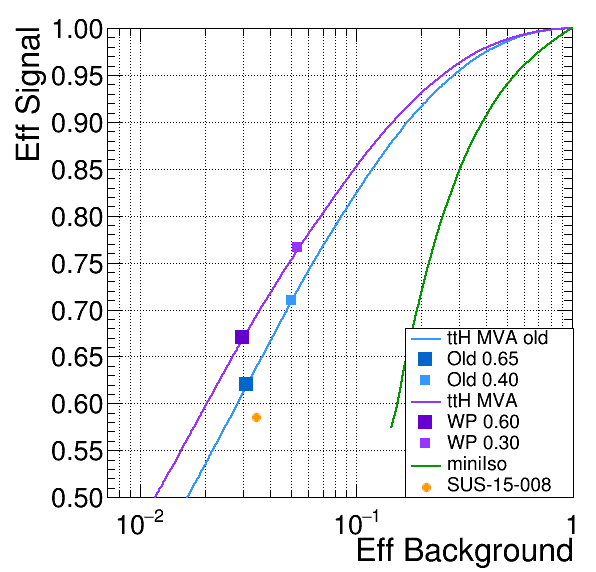
\includegraphics[width=0.40\linewidth]{plots_lepMVA/el_pt_10_25.png}
%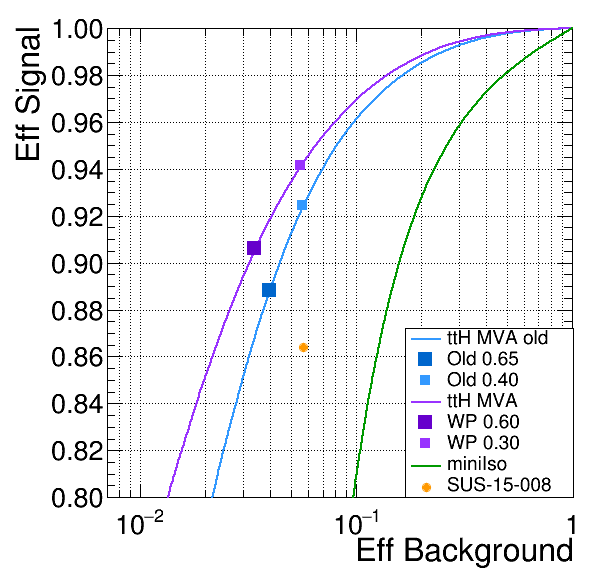
\includegraphics[width=0.40\linewidth]{plots_lepMVA/el_pt_25_inf.png} \\
%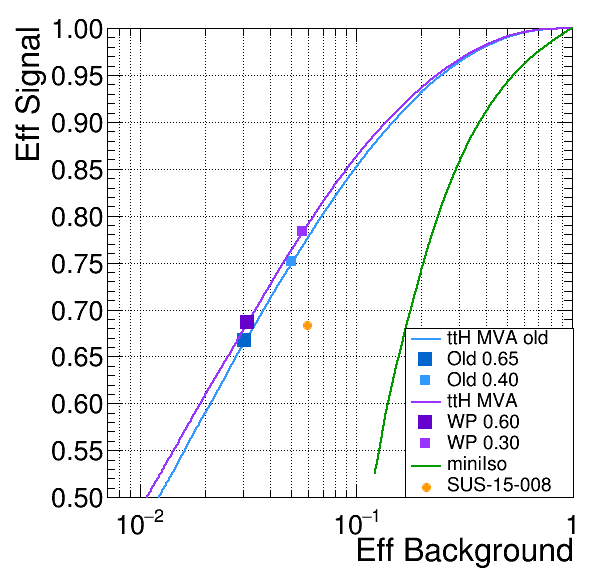
\includegraphics[width=0.40\linewidth]{plots_lepMVA/mu_pt_10_25.png}
%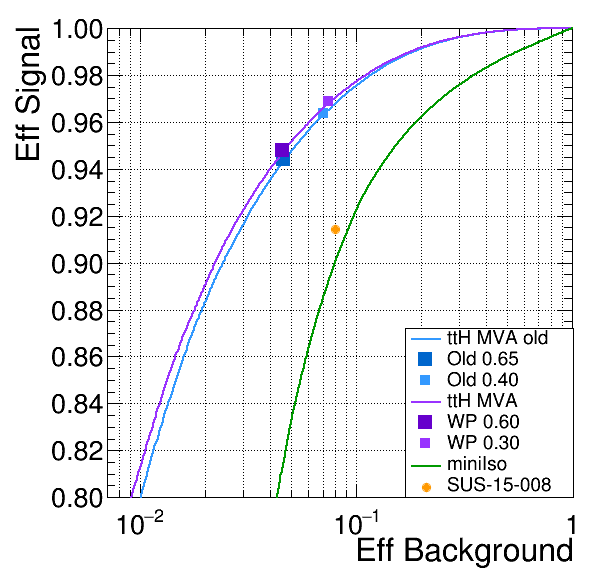
\includegraphics[width=0.40\linewidth]{plots_lepMVA/mu_pt_25_inf.png}
%\caption{The lepton MVA ROCs are shown from top left to bottom right
%for electrons with $10 < \pt < 25$, electrons with $\pt > 25$, muons
%with $10 < \pt < 25$, muons with $\pt > 25$. CMSSW 76X MC is used for this plot.}
%\label{fig:rocsMVA}
%\end{figure}


\subsubsection{Additional requirements}

In the dilepton final state additional requirements on the quality of
the charge assignment are applied to suppress opposite-sign events
in which the charge of one of the leptons is mismeasured. For the electrons we require
consistency between the independent measurements of the charge from
the ECAL supercluster and the tracker, while for the muons we require
the track transverse momentum to be well measured
($\Delta{p_{T}}/p_{T} <0.2$). We will refer to these cuts as \emph{tight-charge}\\
Moreover in order to suppress as much as possible background electrons
from photon conversions we reject electrons with missing hits in the
innermost layer or associated with a successfully reconstructed
conversion vertex~\cite{conversionRejection}.

\subsubsection{ \emph{Loose}, \emph{Fakeable Object}, \emph{Tight} definitions}
Three different selections are used both for the electron and the muon
objects identification: the \emph{Loose}, the \emph{Fakeable Object},
the \emph{Tight} selection. In the description of the analysis
strategy it will be explained for which purposes the different
criteria are used. \\
For reasons that will explained in the data-driven background prediction session,
for the Fakeable Object selections the lepton $\pt$ is
intended to $0.90*\pt(jet)$ with the jet being the one associated to the lepton as defined for the jet-related
variables computation.\\
In Table~\ref{tab:muonIDs} and Table~\ref{tab:eleIDs} all the criteria
on the variables previously described are listed.

\subsection{Validation of lepton identification variables}
We validate the modelling of the lepton identification variables in simulation by looking at three control regions: one enriched in prompt leptons from dileptonic \ttbar, one enriched in non-prompt leptons from semi-leptonic \ttbar, and one enriched in Z+jets events. The first control region is obtained selecting opposite-sign dilepton events with at least two jets and at least one medium b-tagged jet or two loose ones; events with more than two leptons are vetoed. The second control region is obtained selecting same-sign dilepton events with exactly three or four jets, and exactly one medium b-tagged jet, in order to suppress the contributions from $\ttbar\mathrm{V}$ and \ttH, and similarly events with more than two leptons are vetoed.
The third control region is obtained selecting same-flavor and opposite-sign pairs of leptons with higher than 25 and 15 GeV plus a third candidate with pT lower than 50 GeV, for which the transverse mass with the MET is lower than 55 GeV and the MET$<$60 GeV.
In all control regions, the trailing lepton is required only to pass the loose selection, not the lepMVA requirement, so that its properties can be studied in an unbiased way.
A data to simulation comparison is done for the lepton MVA discriminant and some of the more important inputs: the mini-isolation, $\mbox{SIP}_{3D}$, $\ptRatio$, $\ptRel$ and the b-tagging discriminator of the associated jet (Fig.~\ref{fig:lep-distributions-1} and ~\ref{fig:lep-distributions-2}). In all cases, the simulation is normalized to data, scaling all contributions by the same factor. The contribution from \ttbar is split according to the origin of the lepton in the simulation: prompt, non-prompt from B hadron decays ($\cPqb\to\ell_\mathrm{np}$), or non-prompt from other origins  ($\mathrm{j}\to\ell_\mathrm{np}$).
A good agreement between data and simulations is observed overall, while minor discrepancies may be related to the fact that no corrections are applied to the simulation.
% Some small discrepancy is visible mainly for extreme values of the b-tagging discriminator and small $\mbox{SIP}_{3D}$ for non-prompt leptons, which could be also be partially from different relative abunances of leptons from heavy flavour vs light flavour processes in data with respect to simulations, or a slightly different levels of prompt lepton contamination.

\begin{table}[h!]
\centering
\small
\topcaption{
\label{tab:muonIDs}
Requirements on each of the three muon selections. In the cases where
the cut values change between the selections, those values are listed in the table.
Otherwise, whether the cut is applied is indicated.
A few extra requirements are applied for fakeable objects that fail the lepton MVA requirement, to better control the extrapolation in fragmentation and flavour composition: $\ptRatio > 0.5$ (for all), jet $\textrm{CSV} < 0.3$, segmentCompatibility$>$0.3 for muons, electron ID $\textrm{MVA} > 0.0 (0.7)$ for electrons in the barrel (endcaps).}
\begin{tabular}{c|c|c|c}
\hline
\bf{Cut} & \bf{Loose} & \bf{Fakeable Object} & \bf{Tight} \\
\hline
$|\eta| < 2.4$ & \checkmark & \checkmark & \checkmark \\
$\pt$ & $>5$ & $>15$ & $>15$\\
$|d_{xy}| < 0.05$ (cm) & \checkmark & \checkmark & \checkmark \\
$|d_z| < 0.1$ (cm) & \checkmark & \checkmark & \checkmark \\
$\text{SIP}_{3D} < 8$ & \checkmark & \checkmark & \checkmark \\
\miniIso $< 0.4$ & \checkmark & \checkmark & \checkmark \\
is Loose Muon & \checkmark & \checkmark & \checkmark \\
%\ptRatio & -- & $>0.3\dagger$ / -- &  -- \\
jet CSV  & -- & $< 0.8484$ & $ < 0.8484$ \\
%mva electron ID  & -- & $\ddagger$ & -- \\
is Medium Muon & -- & -- & \checkmark \\
tight-charge & -- & -- & \checkmark \\
lepMVA $> 0.90$ & -- & -- & \checkmark \\
\hline
\end{tabular}
\end{table}


\begin{table}
\centering
\small
\topcaption{
\label{tab:eleIDs}
Requirements on each of the three electron selections. In the cases where the cut values change between the selections, those values are listed in the table. Otherwise, whether the cut is applied is indicated. In some cases, the cut values change for different $\eta$ ranges. These ranges are $0 < |\eta| < 0.8$, $0.8 < |\eta| < 1.479$, and $1.479 < |\eta| < 2.5$ and the respective cut values are given in the form (value$_1$, value$_2$, value$_3$). Cuts marked with $\dagger$ are applied only to objects failing the tight selection.
}
\resizebox{1.0\linewidth}{!}{
\begin{tabular}{c|c|c|c}
\hline
\bf{Cut} & \bf{Loose} & \bf{Fakeable Object} & \bf{Tight} \\
\hline
$|\eta| < 2.5$ & \checkmark & \checkmark & \checkmark \\
$\pt$ & $>7$ & $>15$ & $>15$ 2lss(3l) \\
$|d_{xy}| < 0.05$ (cm) & \checkmark & \checkmark & \checkmark \\
$|d_z| < 0.1$ (cm) & \checkmark & \checkmark & \checkmark \\
$\text{SIP}_{3D} < 8$ & \checkmark & \checkmark & \checkmark \\
\miniIso $< 0.4$ & \checkmark & \checkmark & \checkmark \\
MVA ID $> (0.0, 0.0, 0.7)$ & \checkmark & \checkmark & \checkmark \\
$\sigma_{i\eta i\eta} <(0.011,0.011,0.030)$ & -- & \checkmark & \checkmark \\ %& for corr. $\pt>30$ & for corr. $\pt>30$ \\
H/E $< (0.10,0.10,0.07)$ & -- & \checkmark & \checkmark \\ %& for corr. $\pt>30$ & for corr. $\pt>30$ \\
$\Delta\eta_{\textrm in} < (0.01, 0.01, 0.008)$ & -- & \checkmark & \checkmark \\ %& for corr. $\pt>30$ & for corr. $\pt>30$ \\
$\Delta\phi_{\textrm in} < (0.04, 0.04, 0.07)$ & -- & \checkmark & \checkmark \\ %& for corr. $\pt>30$ & for corr. $\pt>30$ \\
$-0.05 < 1/E-1/p < (0.010,0.010,0.005)$ & -- & \checkmark & \checkmark \\ %& for corr. $\pt>30$ & for corr. $\pt>30$ \\
\ptRatio & -- & $>0.5\dagger$ / -- & -- \\
jet CSV  & -- & $< 0.3 \dagger$ / $< 0.8484$ & $ < 0.8484$ \\
tight-charge & -- & -- & \checkmark \\
conversion rejection & -- & -- & \checkmark \\
Number of missing hits & $<2$ & $== 0$ & $== 0$ \\
lepMVA $> 0.90$ & -- & -- & \checkmark \\
\hline
\end{tabular}}
\end{table}

\begin{figure}
        \centering
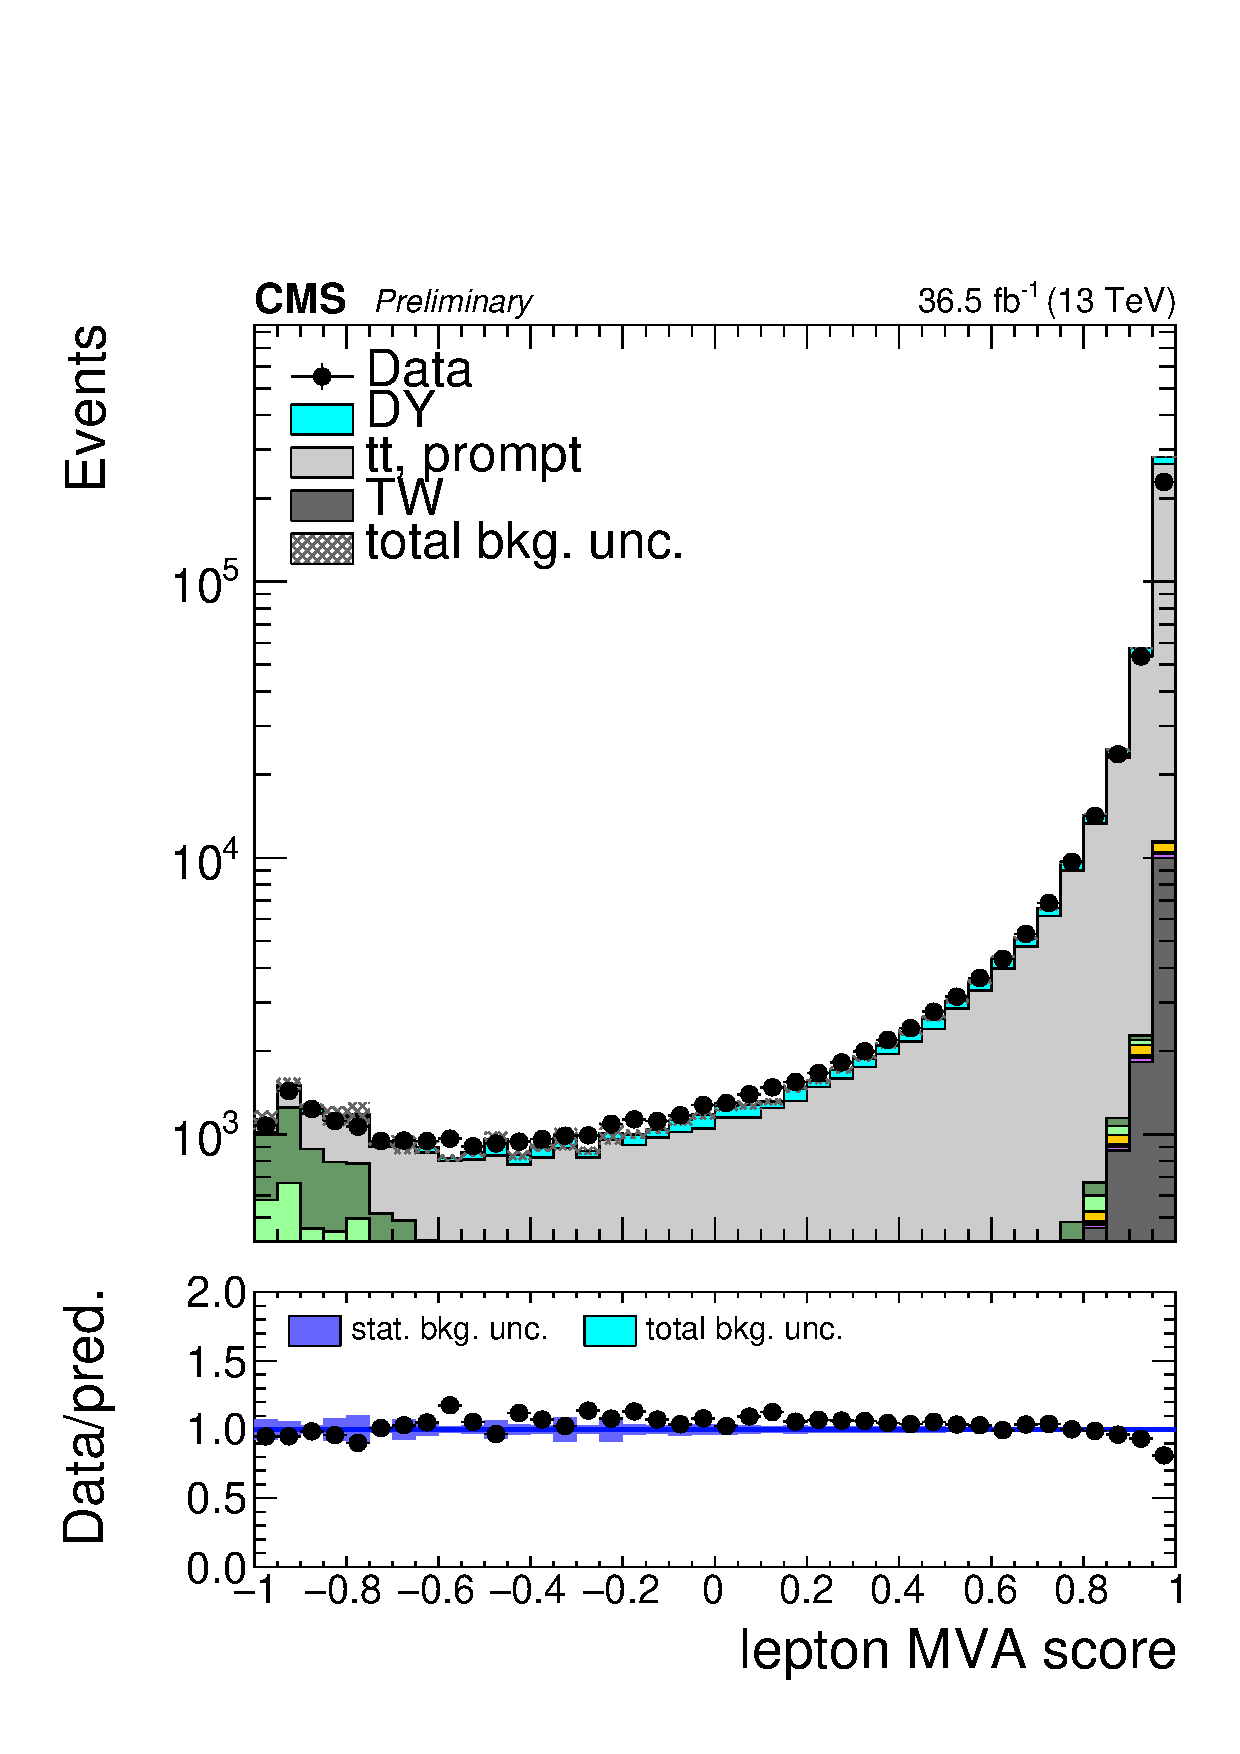
\includegraphics[width=0.32\textwidth]{plots_controlregions/leptons/lep_mvaTTH_log_prompt.pdf}
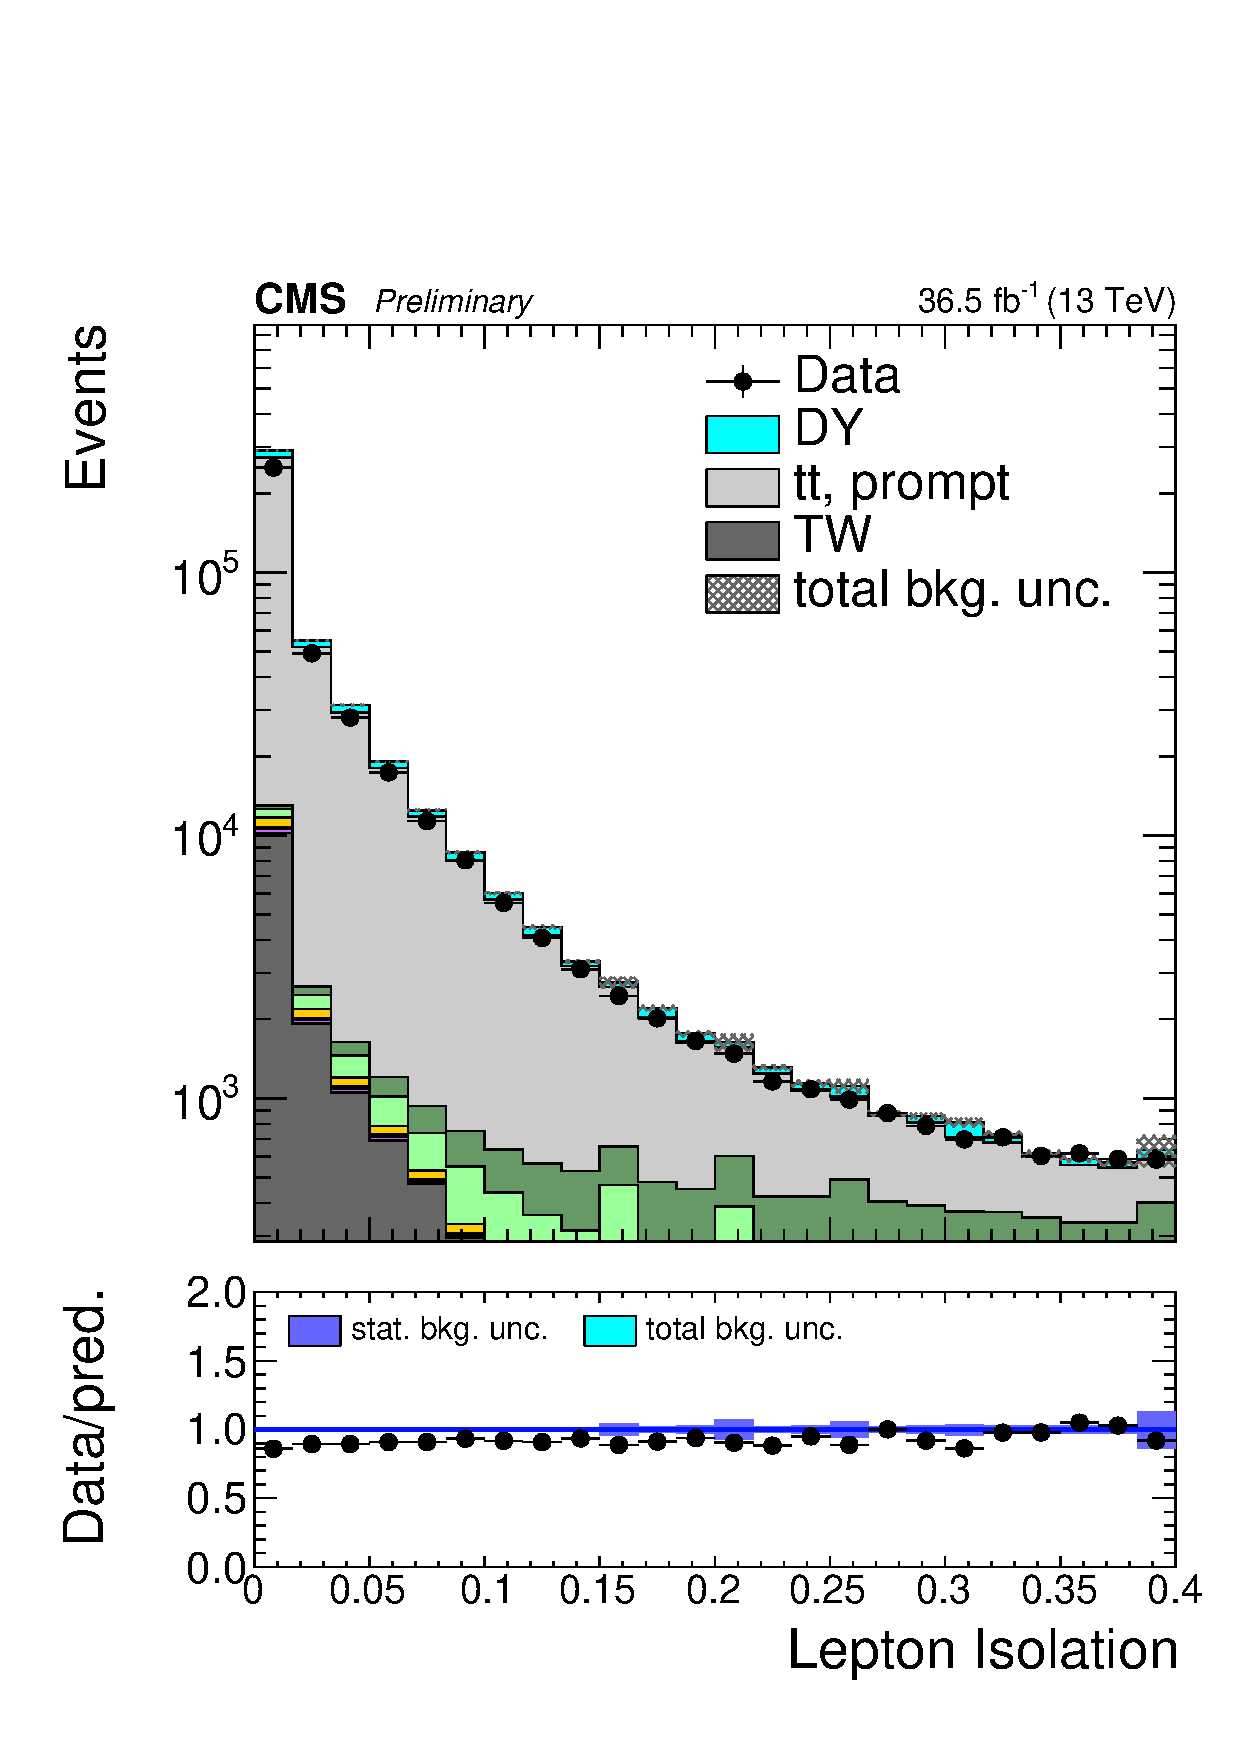
\includegraphics[width=0.32\textwidth]{plots_controlregions/leptons/lep_miniRelIso_log_prompt.pdf}
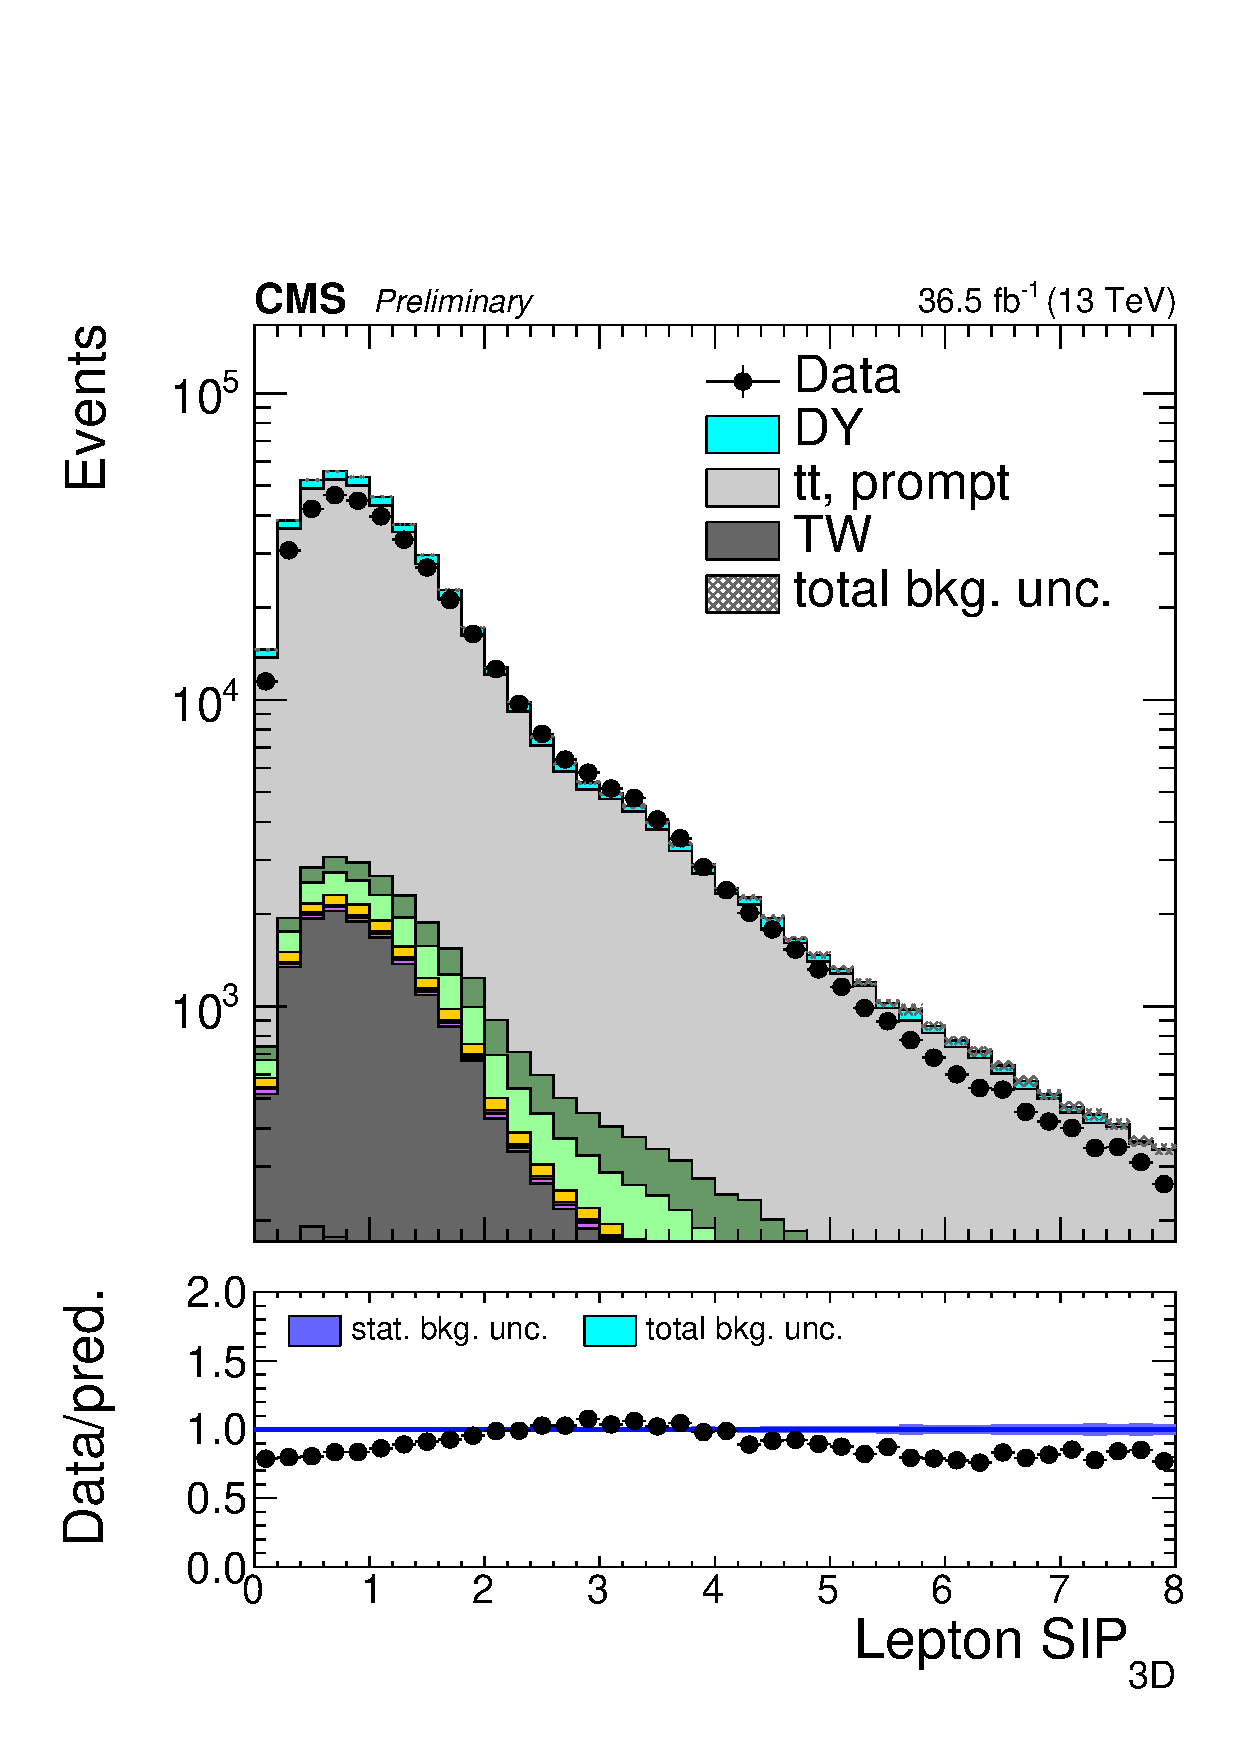
\includegraphics[width=0.32\textwidth]{plots_controlregions/leptons/lep_sip3d_log_prompt.pdf}\\
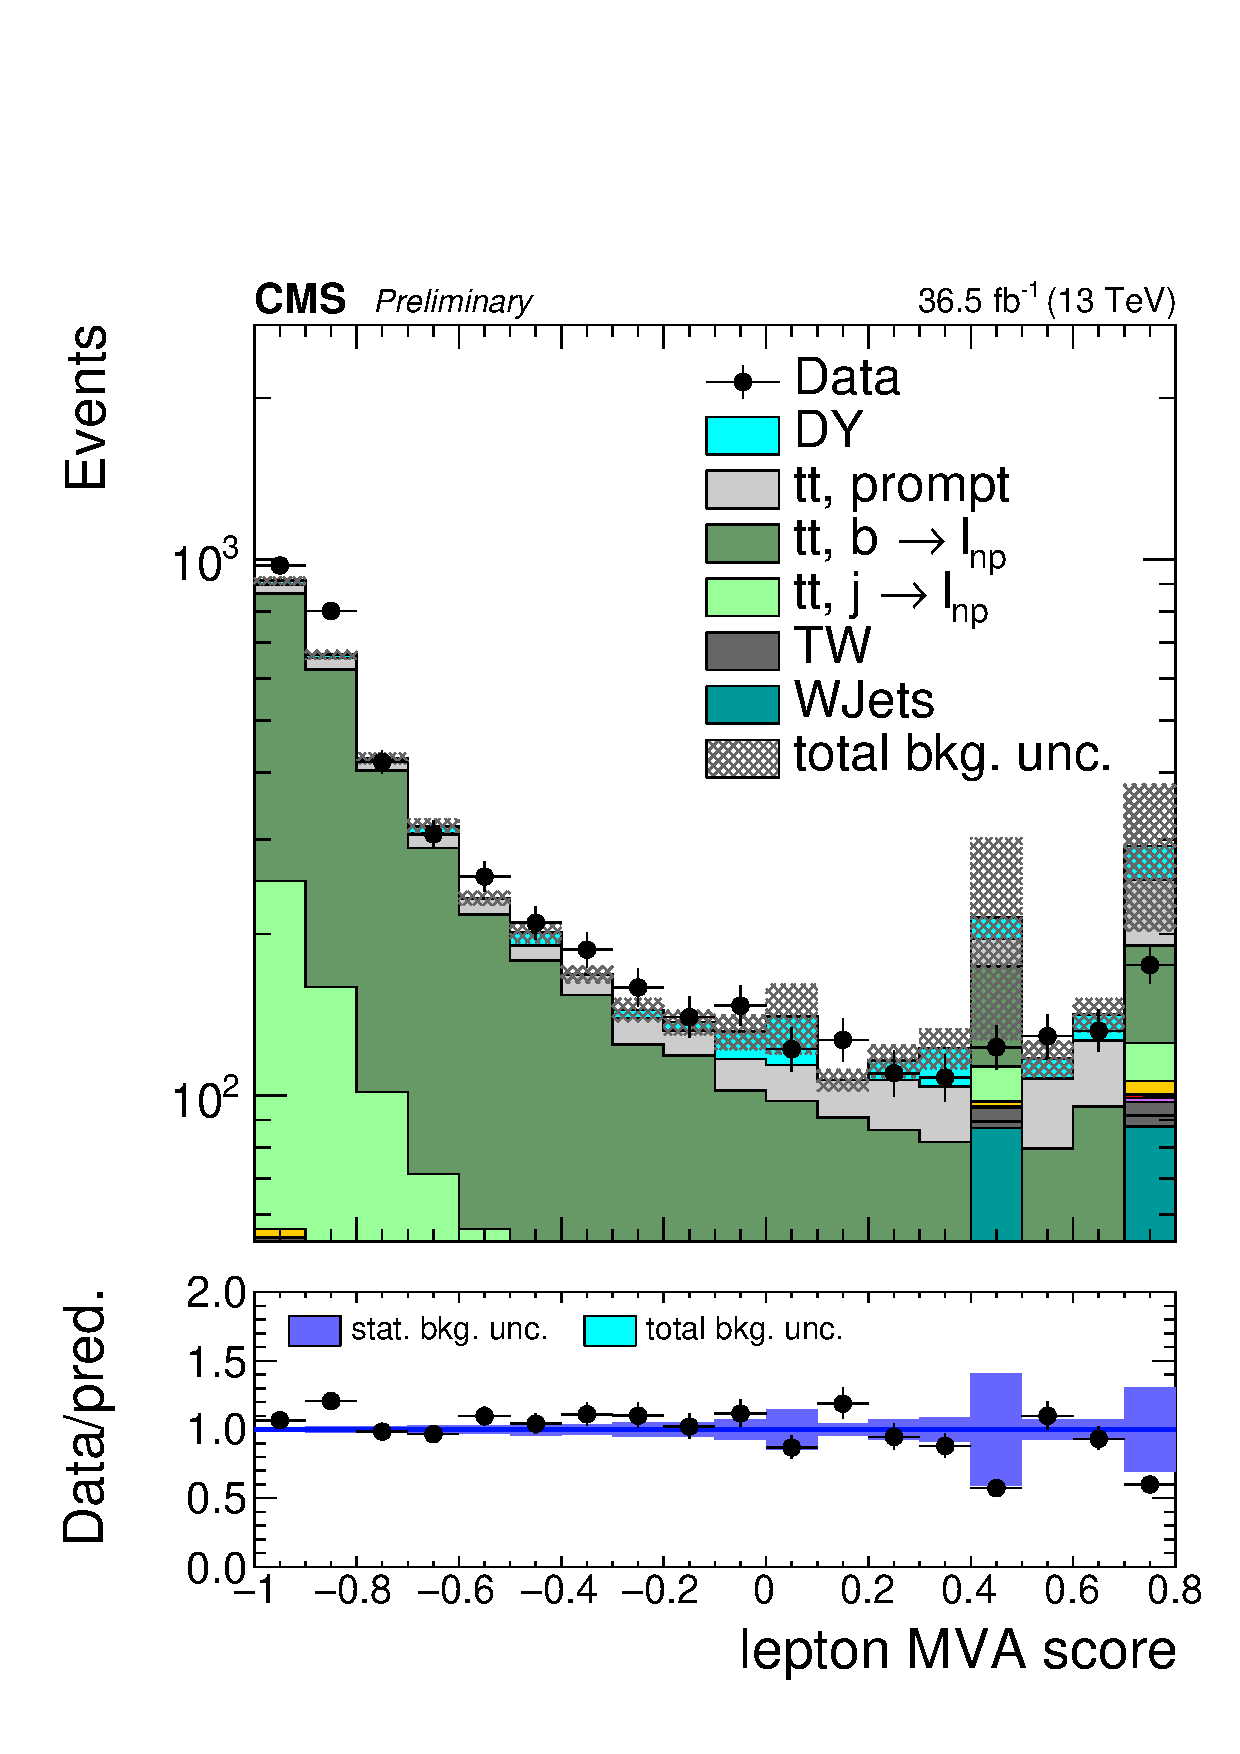
\includegraphics[width=0.32\textwidth]{plots_controlregions/leptons/lep_mvaTTH_log.pdf}
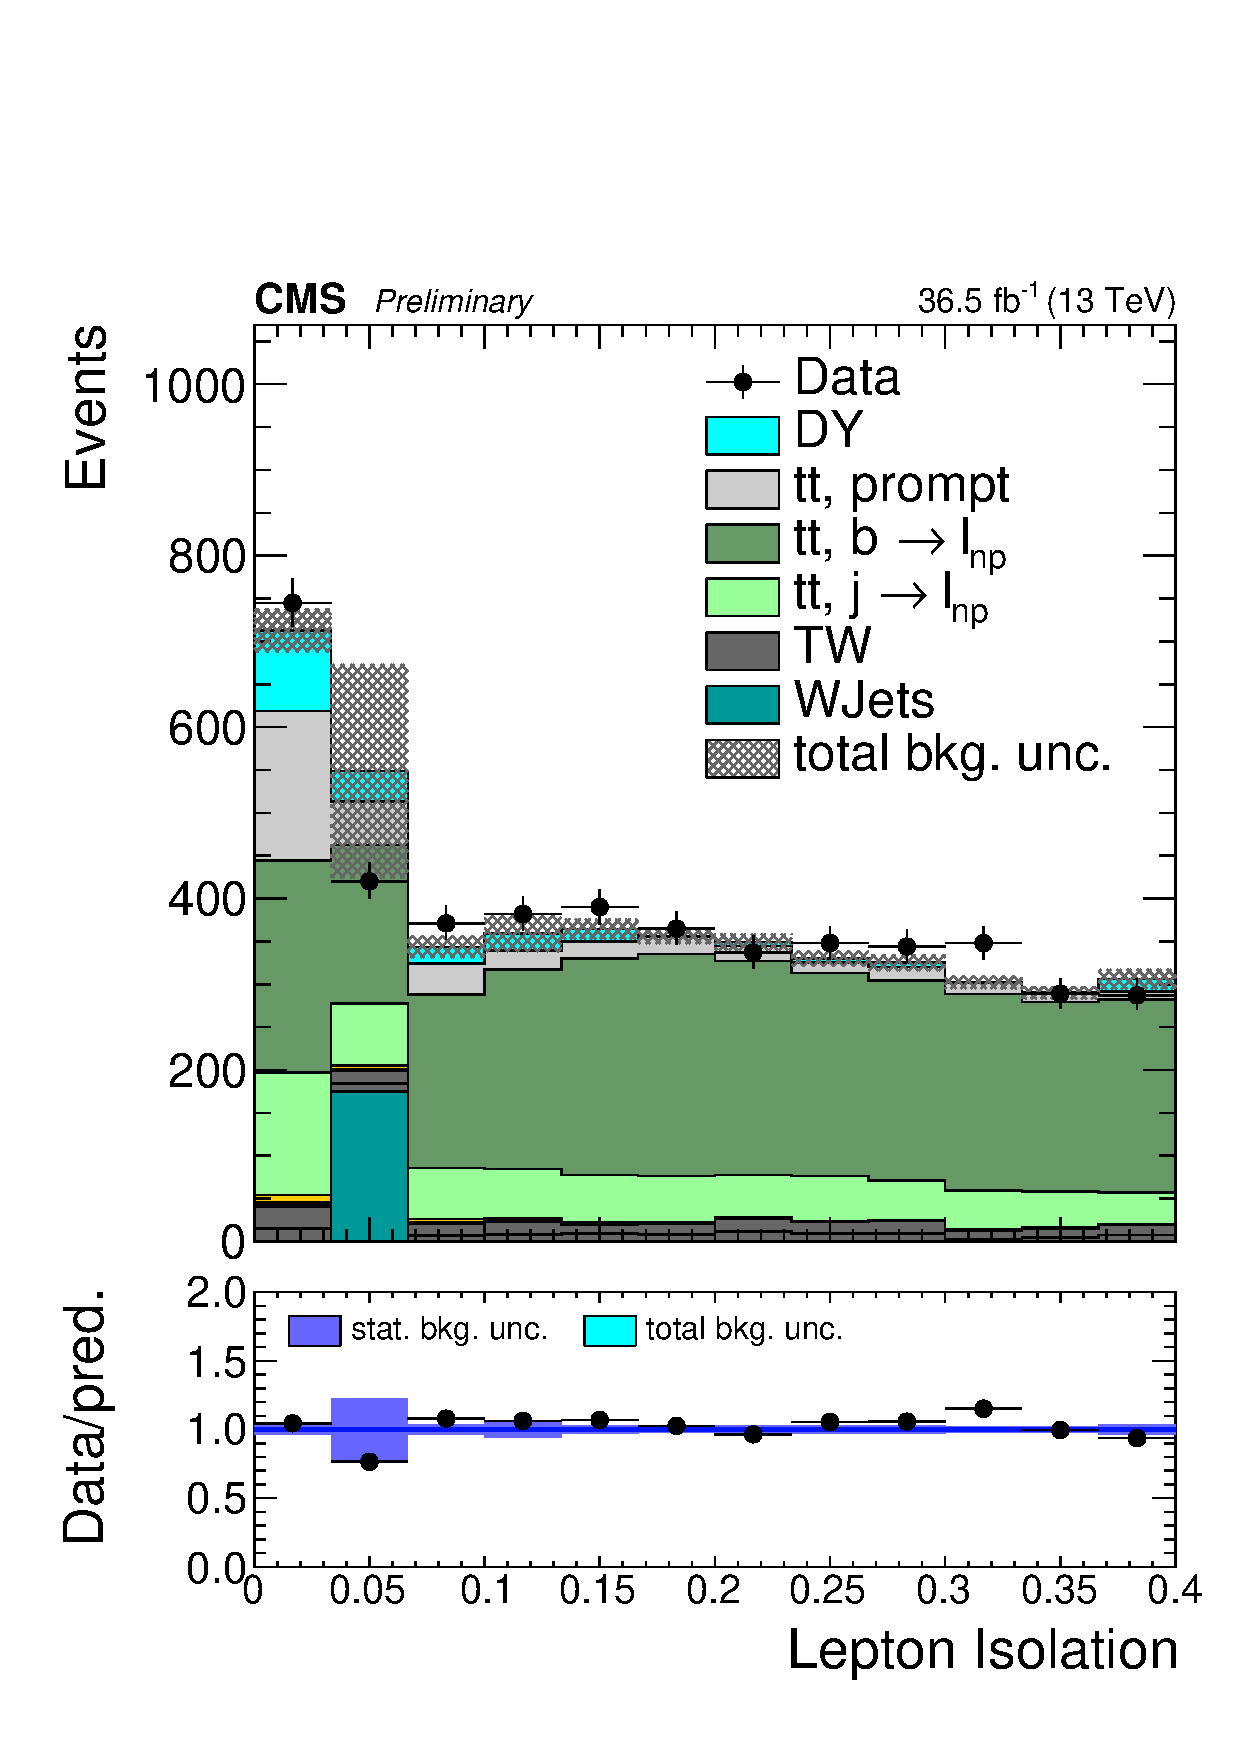
\includegraphics[width=0.32\textwidth]{plots_controlregions/leptons/lep_miniRelIso.pdf}
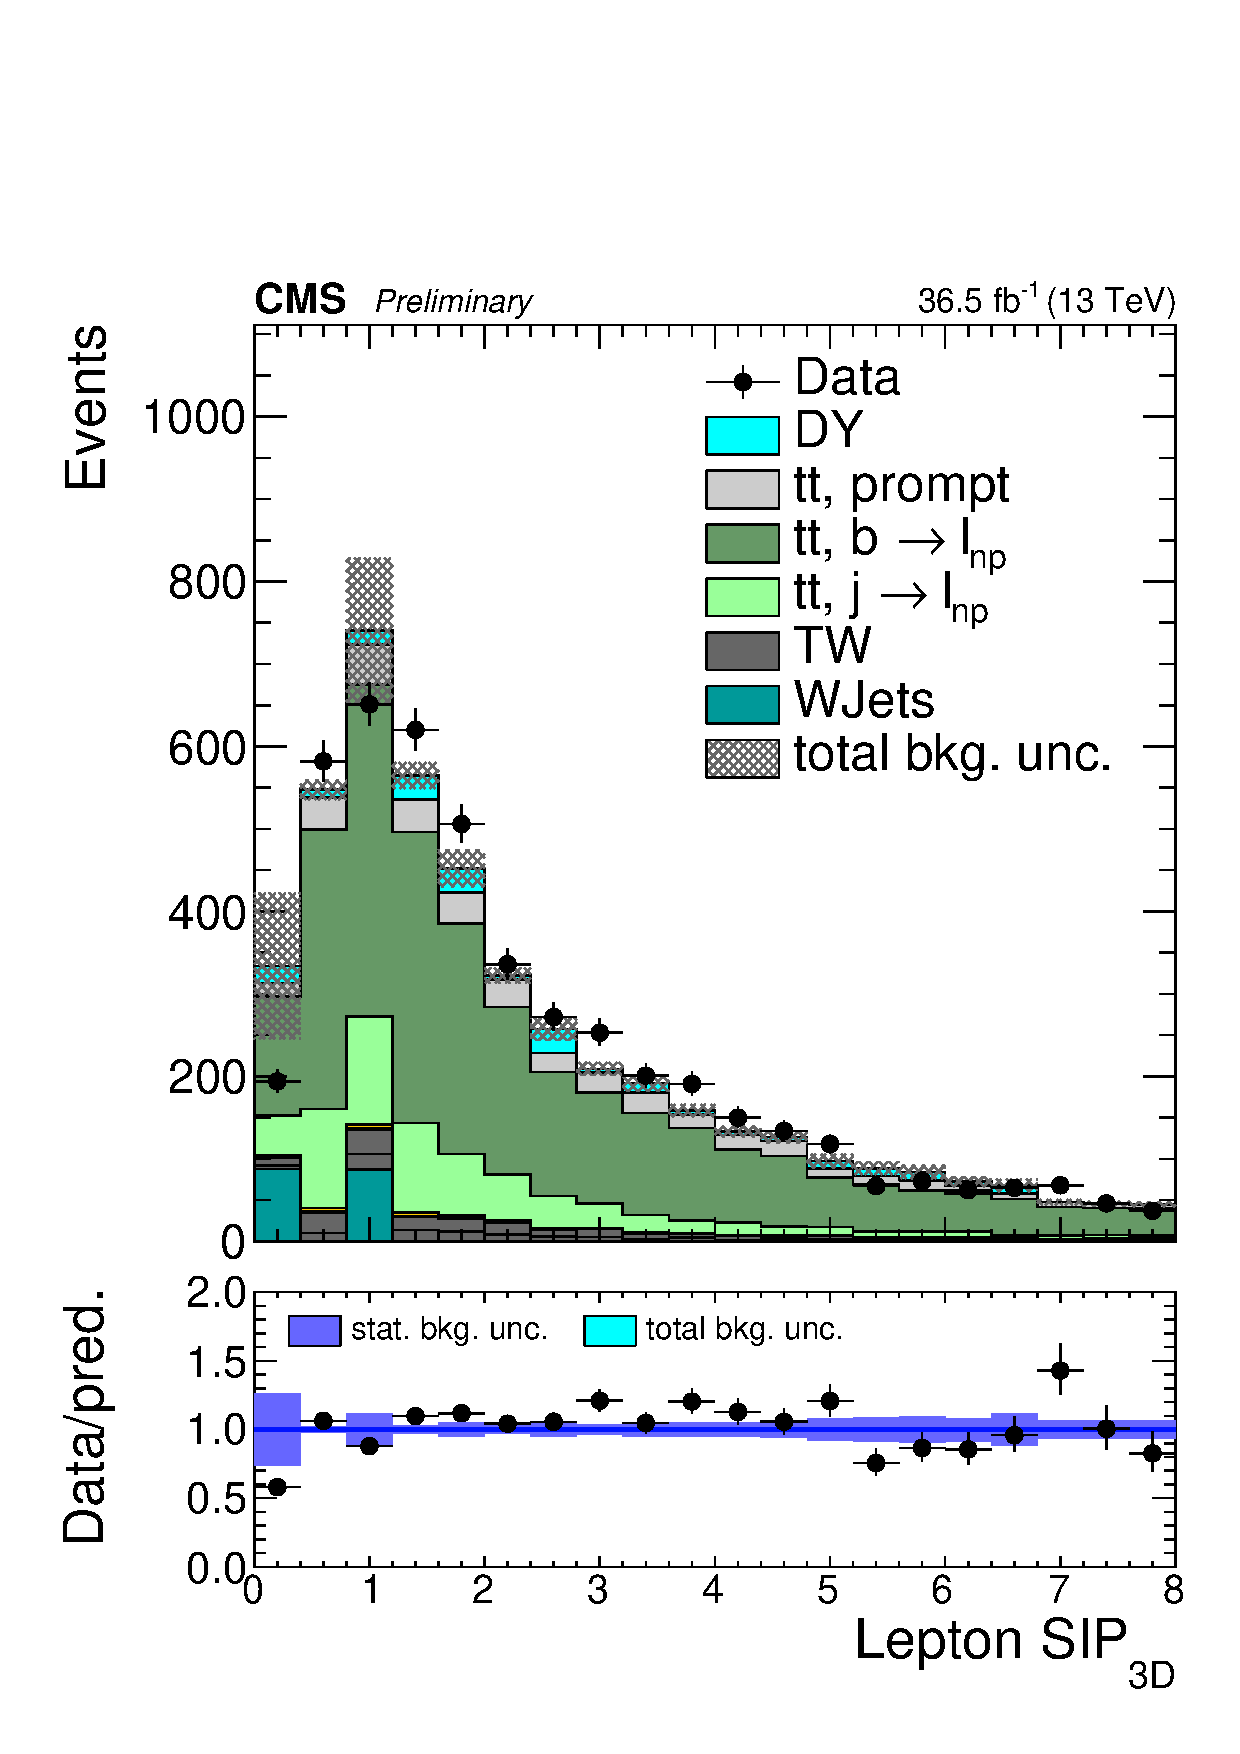
\includegraphics[width=0.32\textwidth]{plots_controlregions/leptons/lep_sip3d.pdf}\\
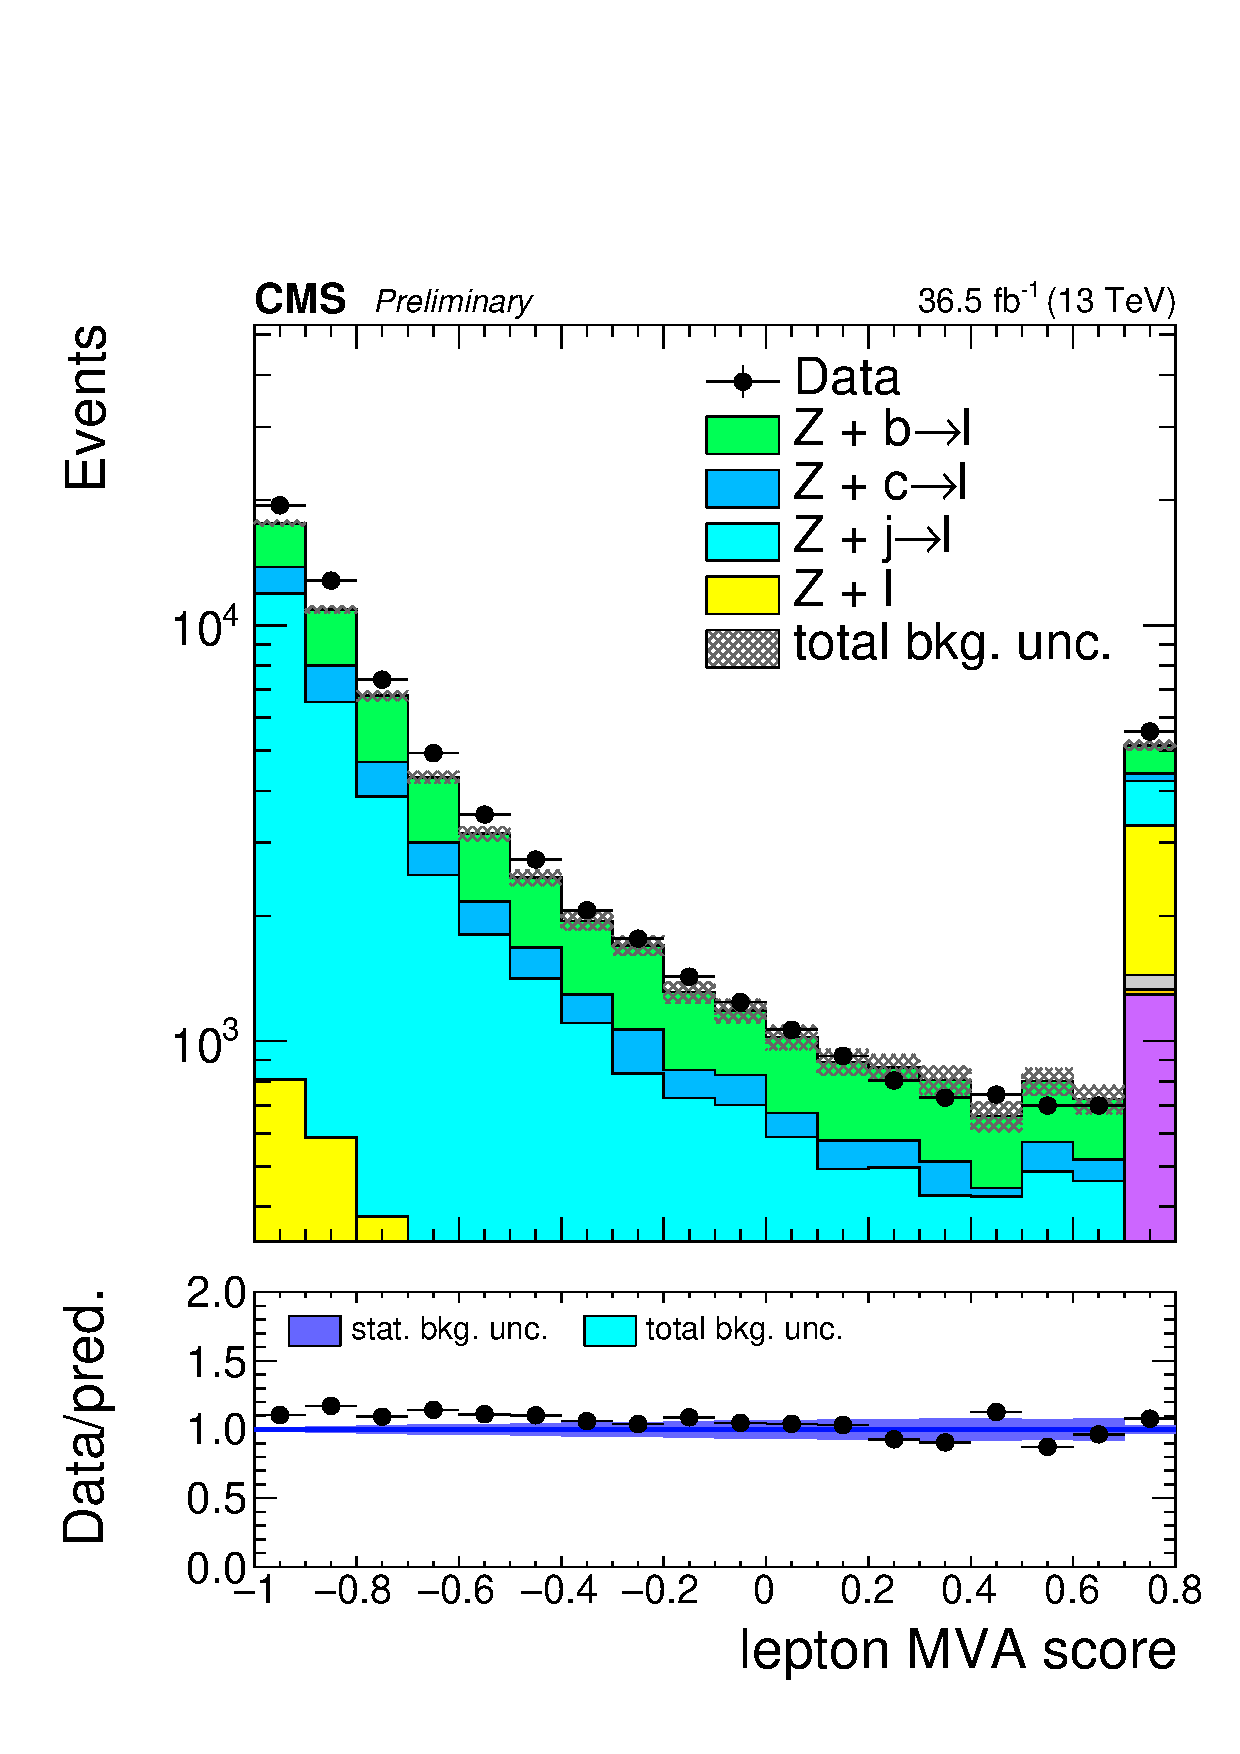
\includegraphics[width=0.32\textwidth]{plots_controlregions/leptons/lep_mvaTTH_log_Zl.pdf}
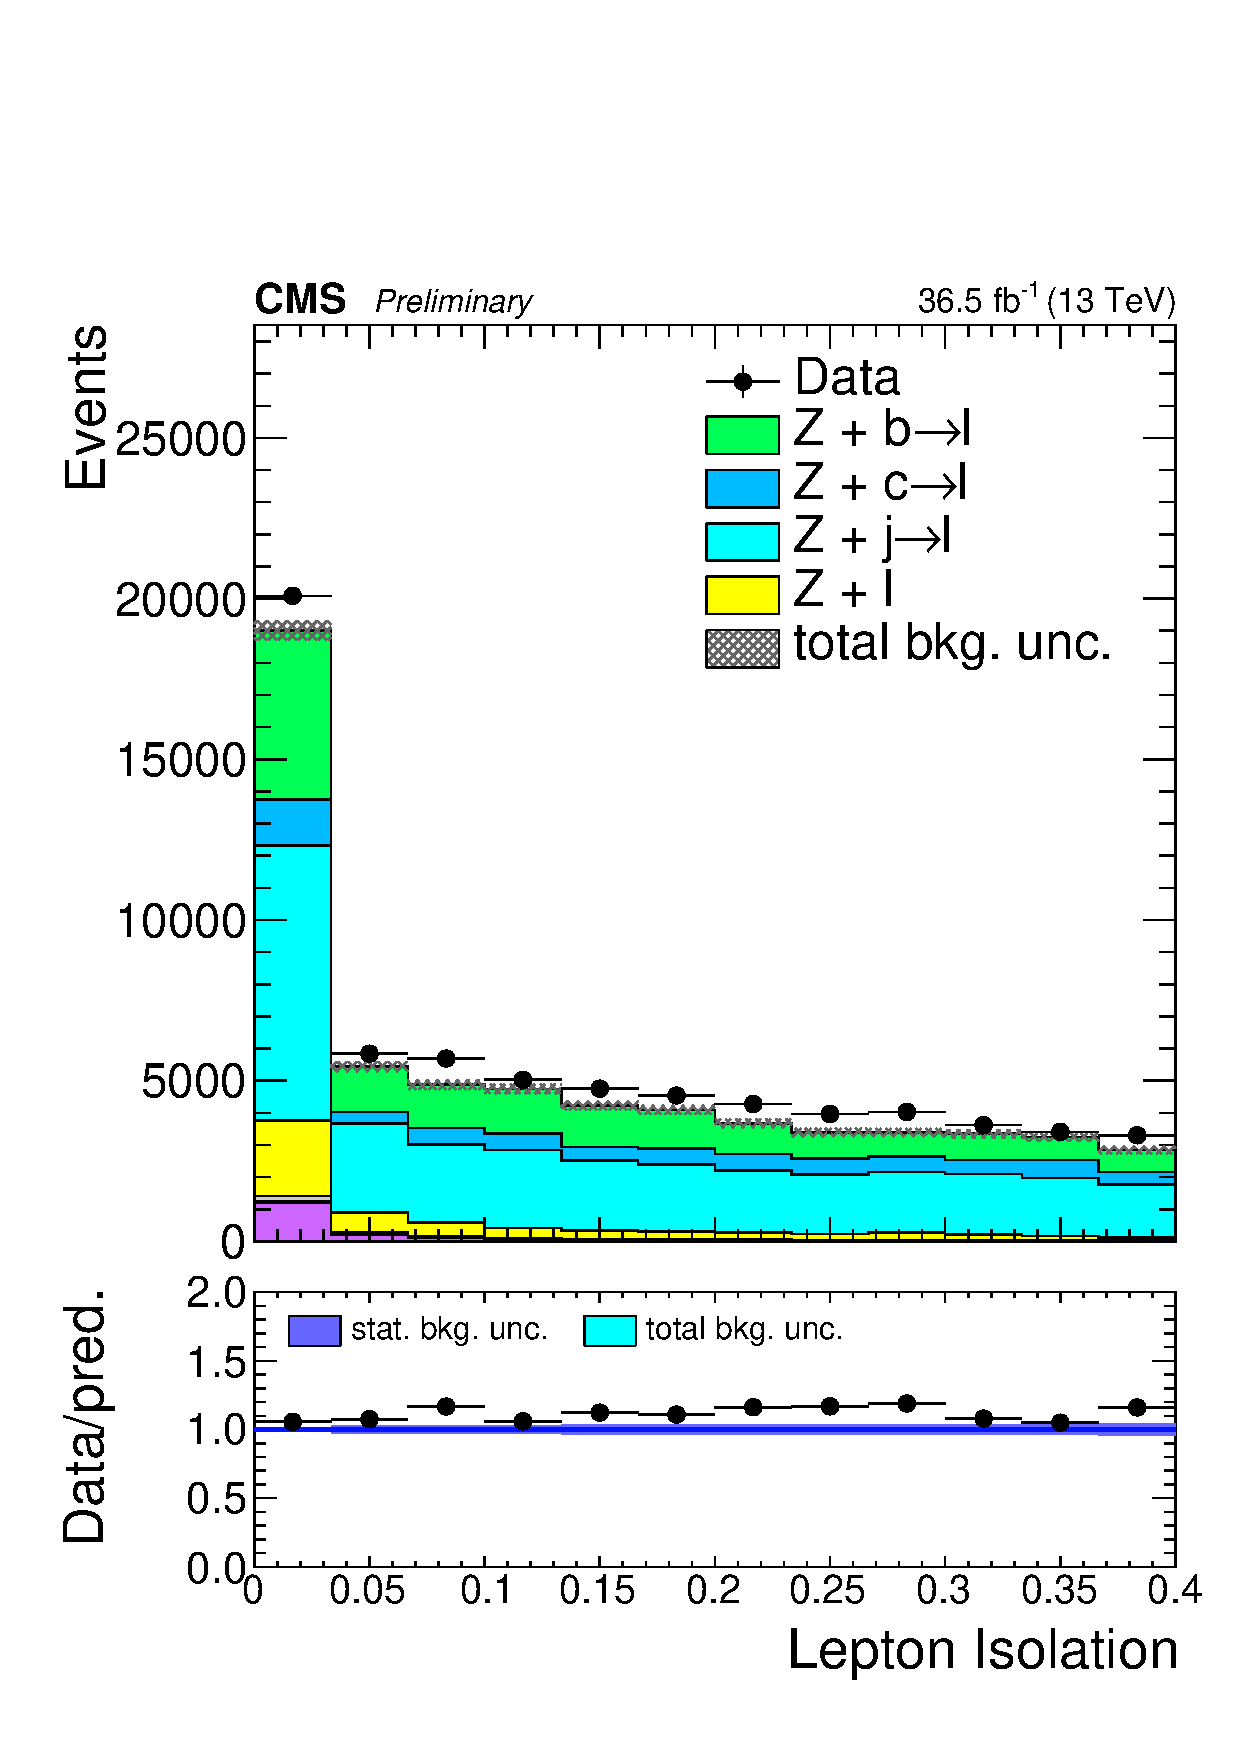
\includegraphics[width=0.32\textwidth]{plots_controlregions/leptons/lep_miniRelIso_Zl.pdf}
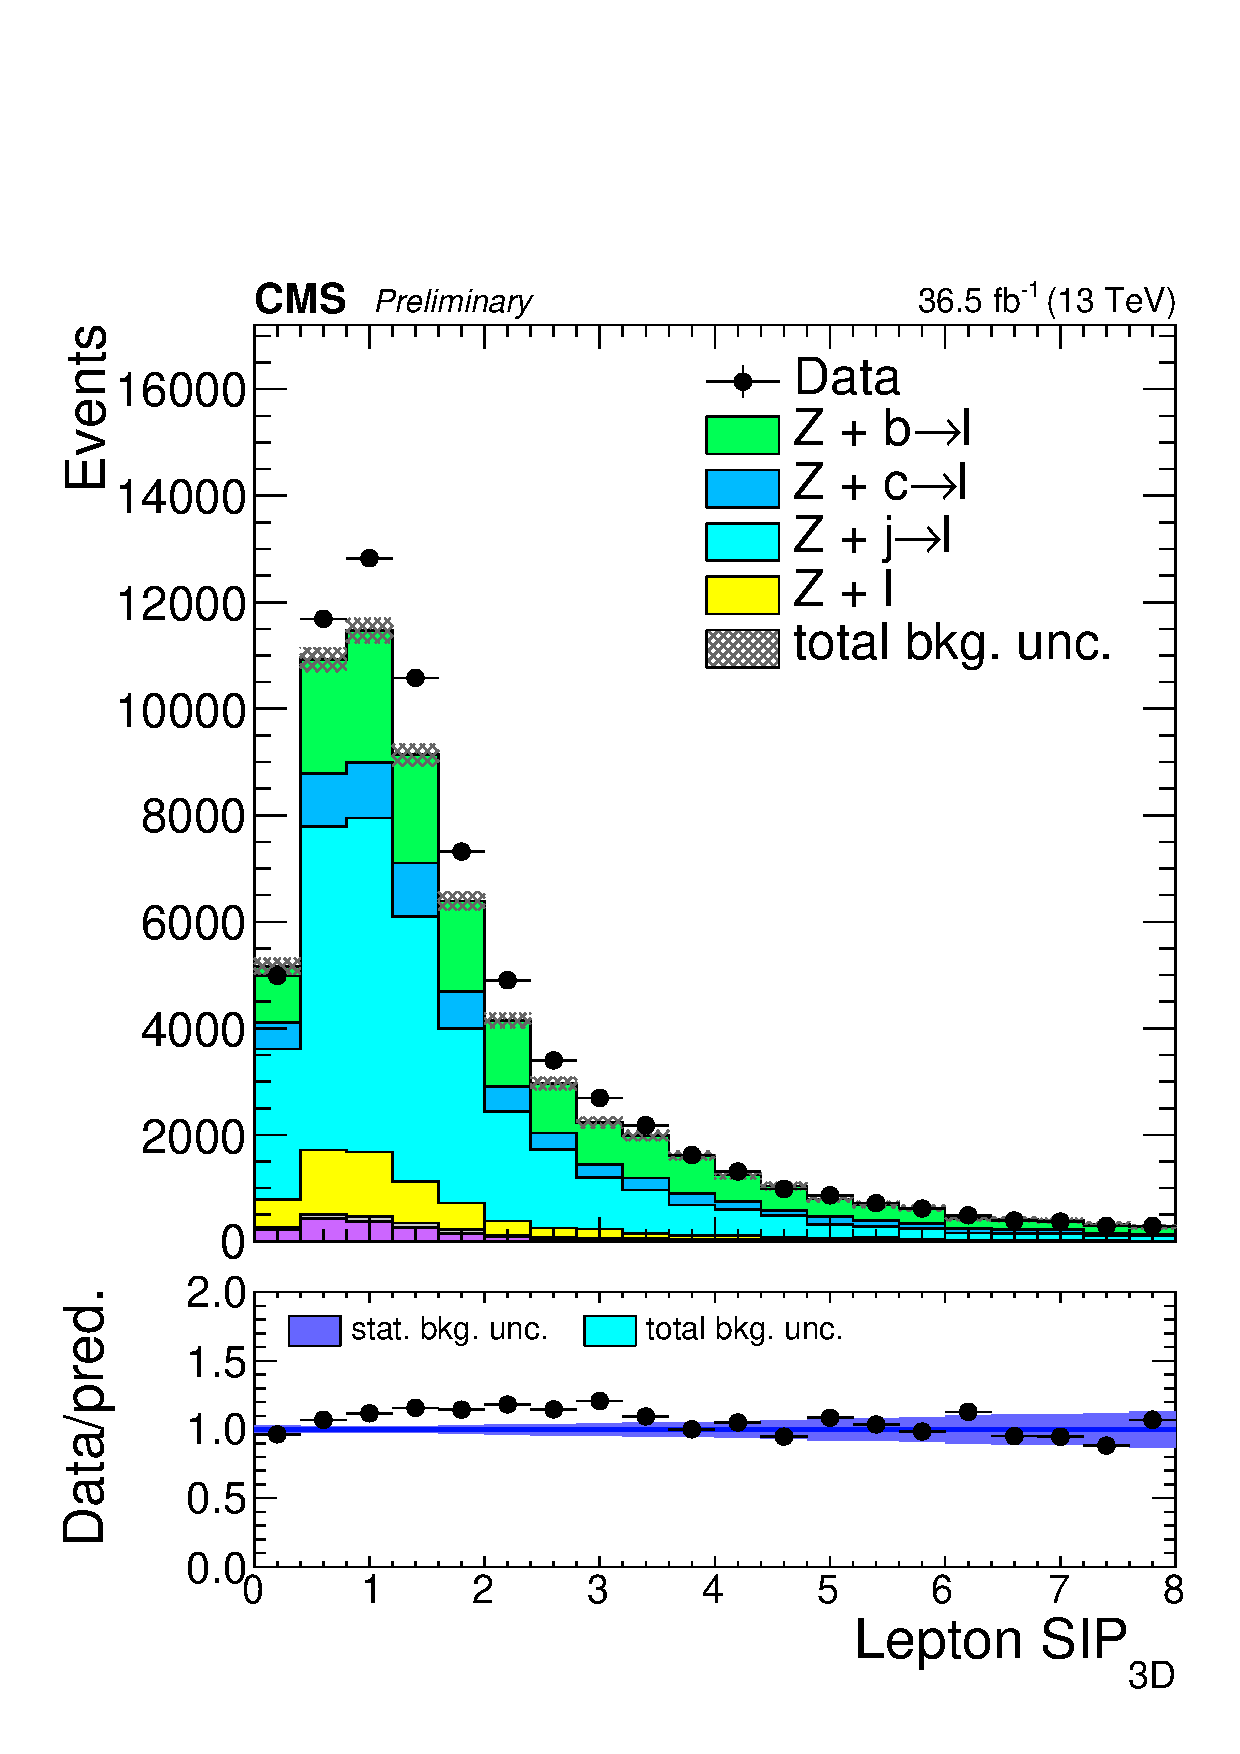
\includegraphics[width=0.32\textwidth]{plots_controlregions/leptons/lep_sip3d_Zl.pdf}
        \caption{Comparison of the distributions for the lepton MVA (left), mini-isolation (center), and $\mbox{SIP}_{3D}$ (right) between data and simulations in control regions enriched in prompt leptons (top), non-prompt leptons (center), and Z+jets events (bottom), as described in the text. The uncertainty shown on the simulation is only statistical.}
        \label{fig:lep-distributions-1}
\end{figure}

\begin{figure}
        \centering
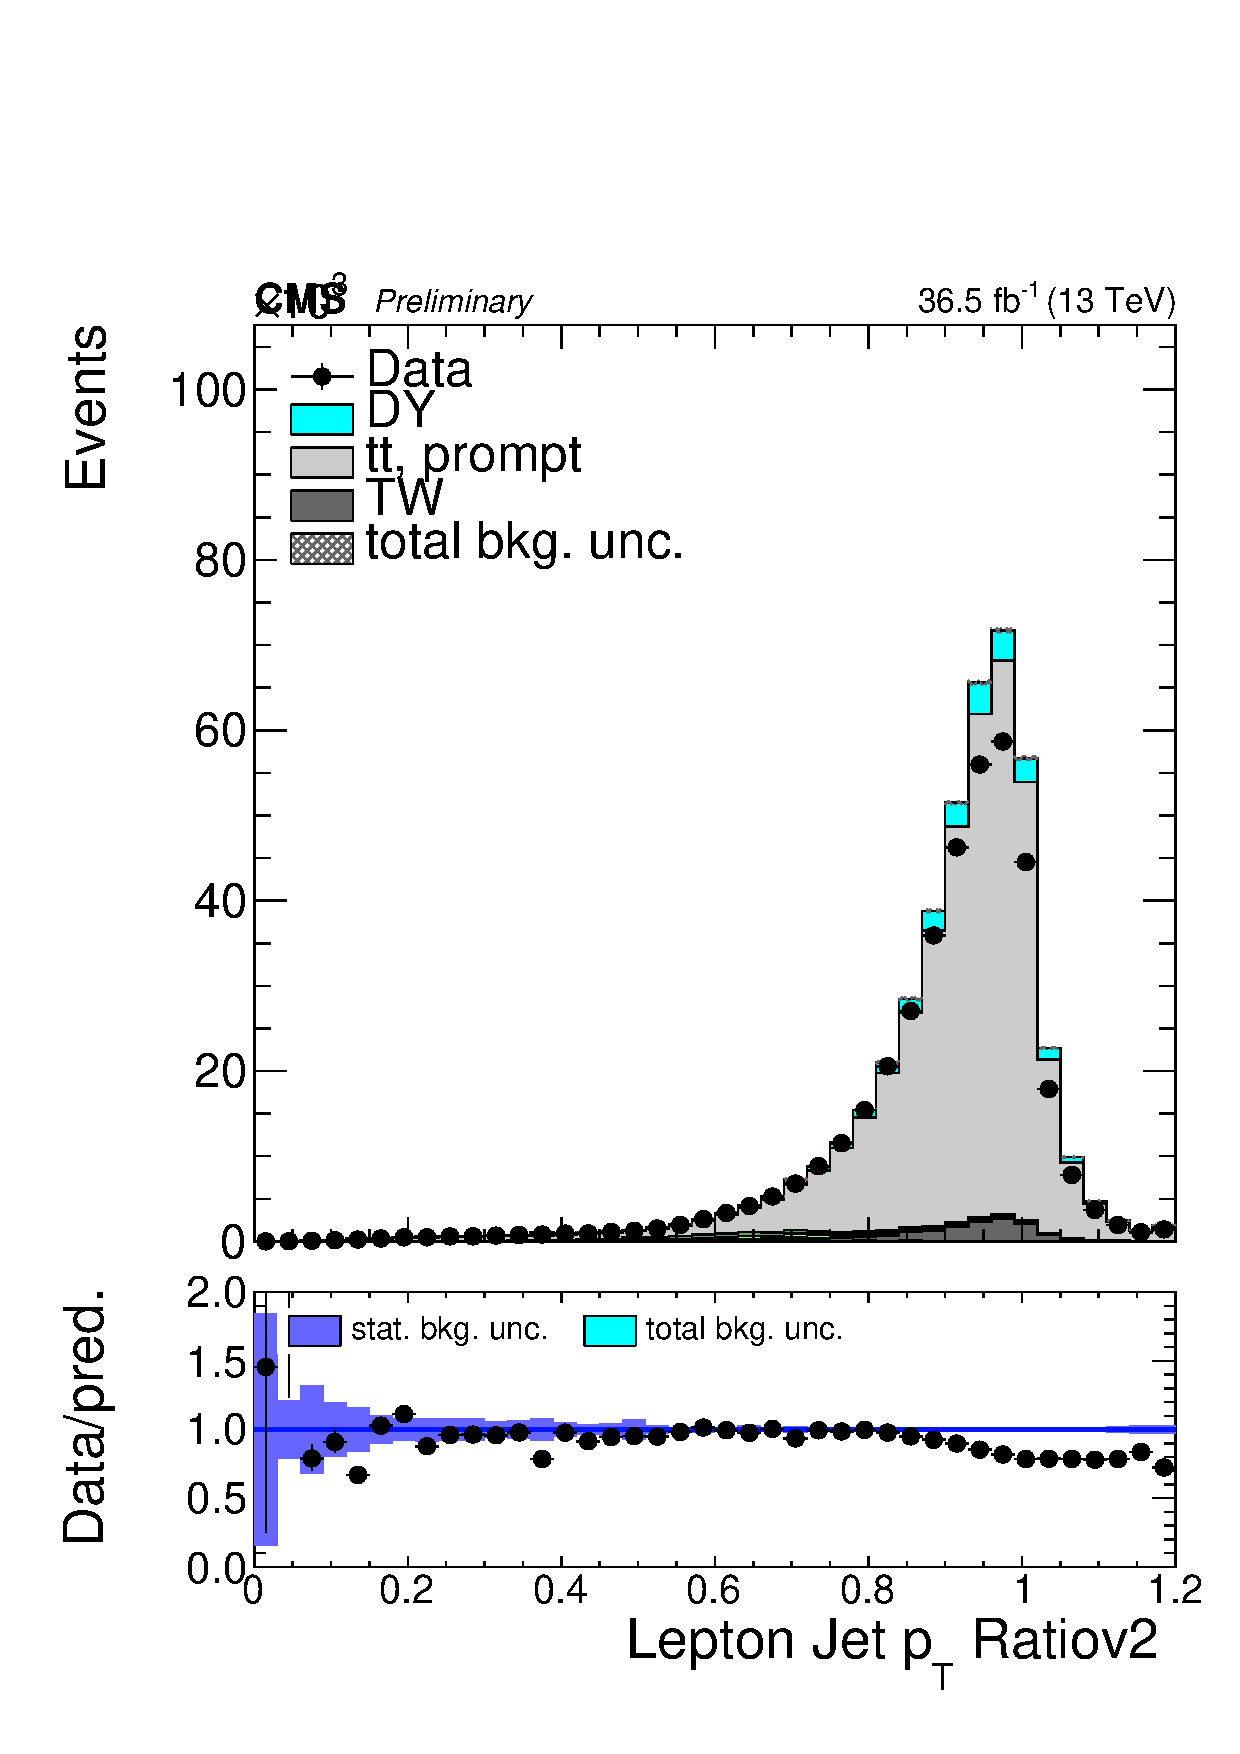
\includegraphics[width=0.32\textwidth]{plots_controlregions/leptons/lep_jetPtRatiov2_prompt.pdf}
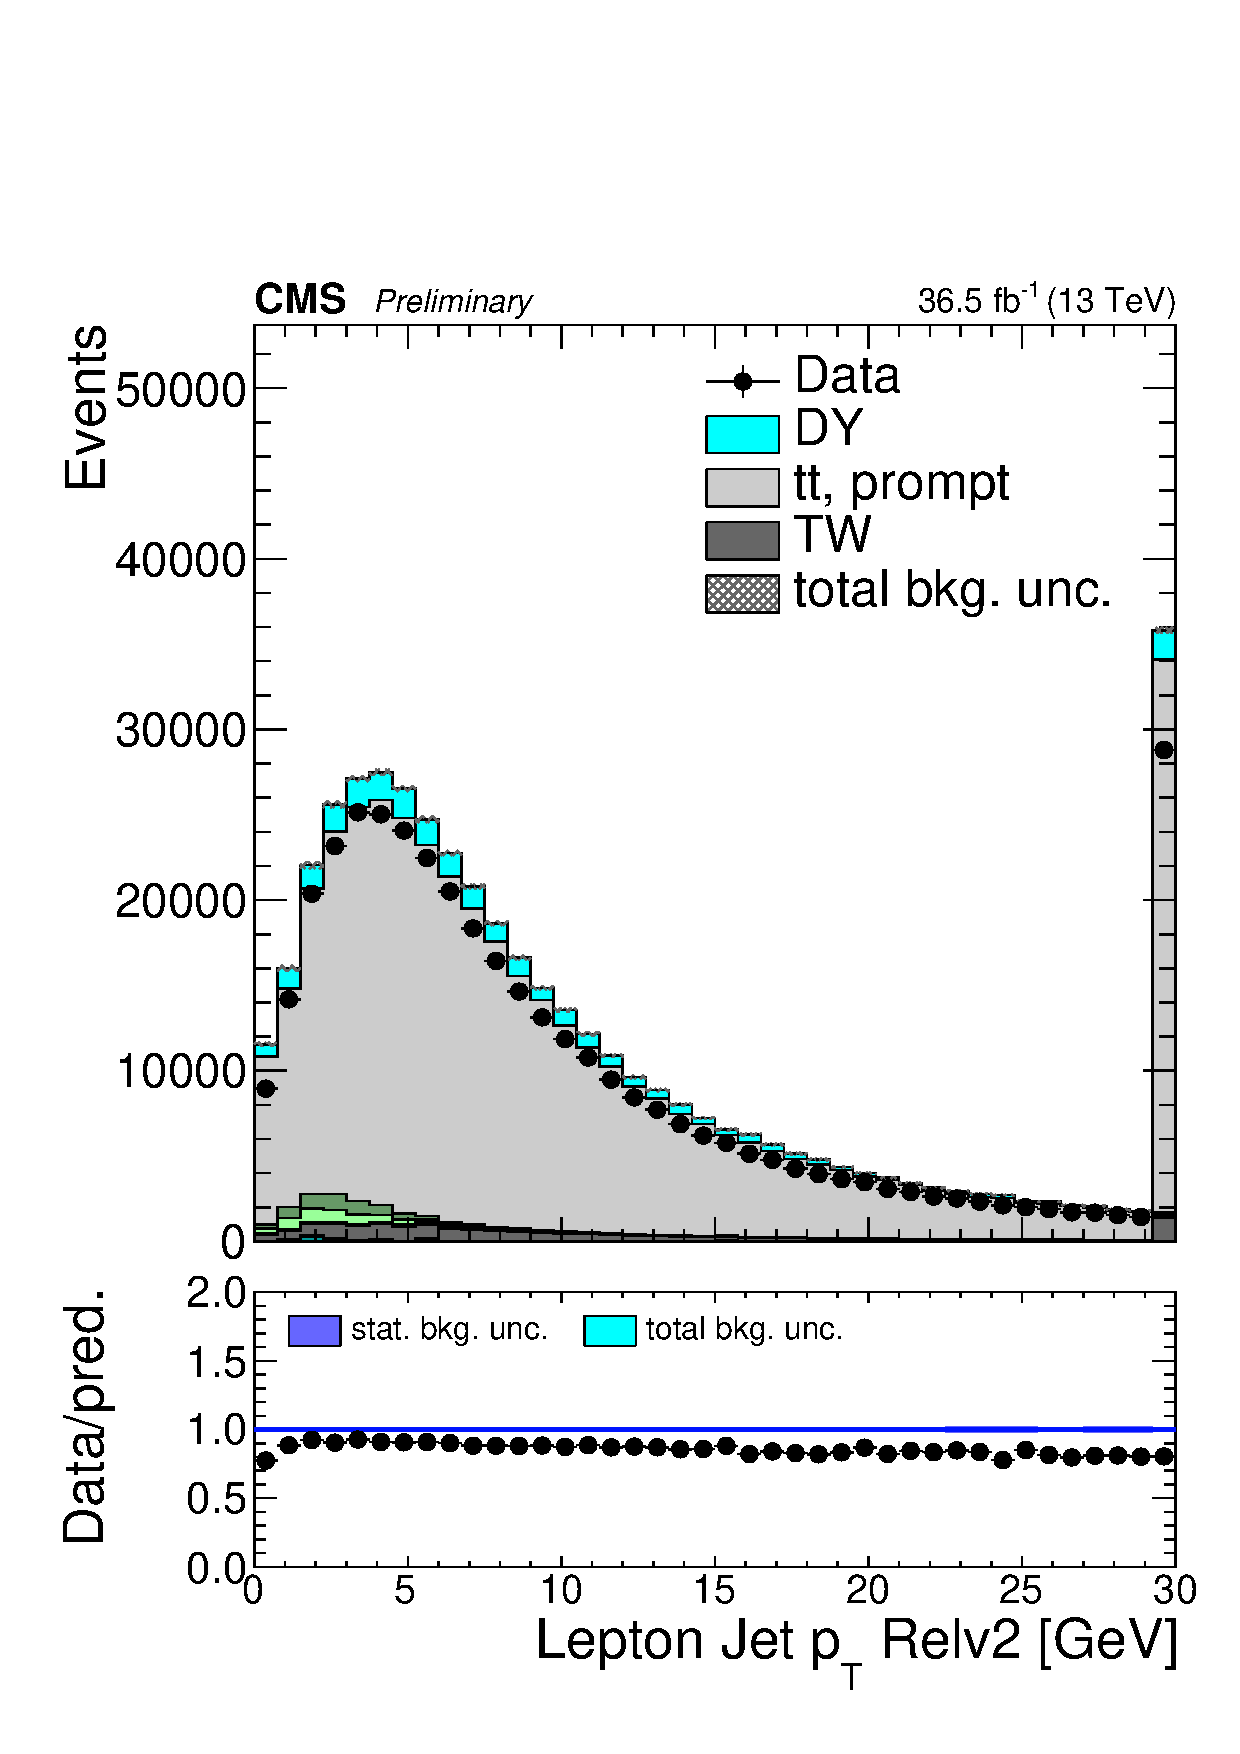
\includegraphics[width=0.32\textwidth]{plots_controlregions/leptons/lep_jetPtRelv2_prompt.pdf}
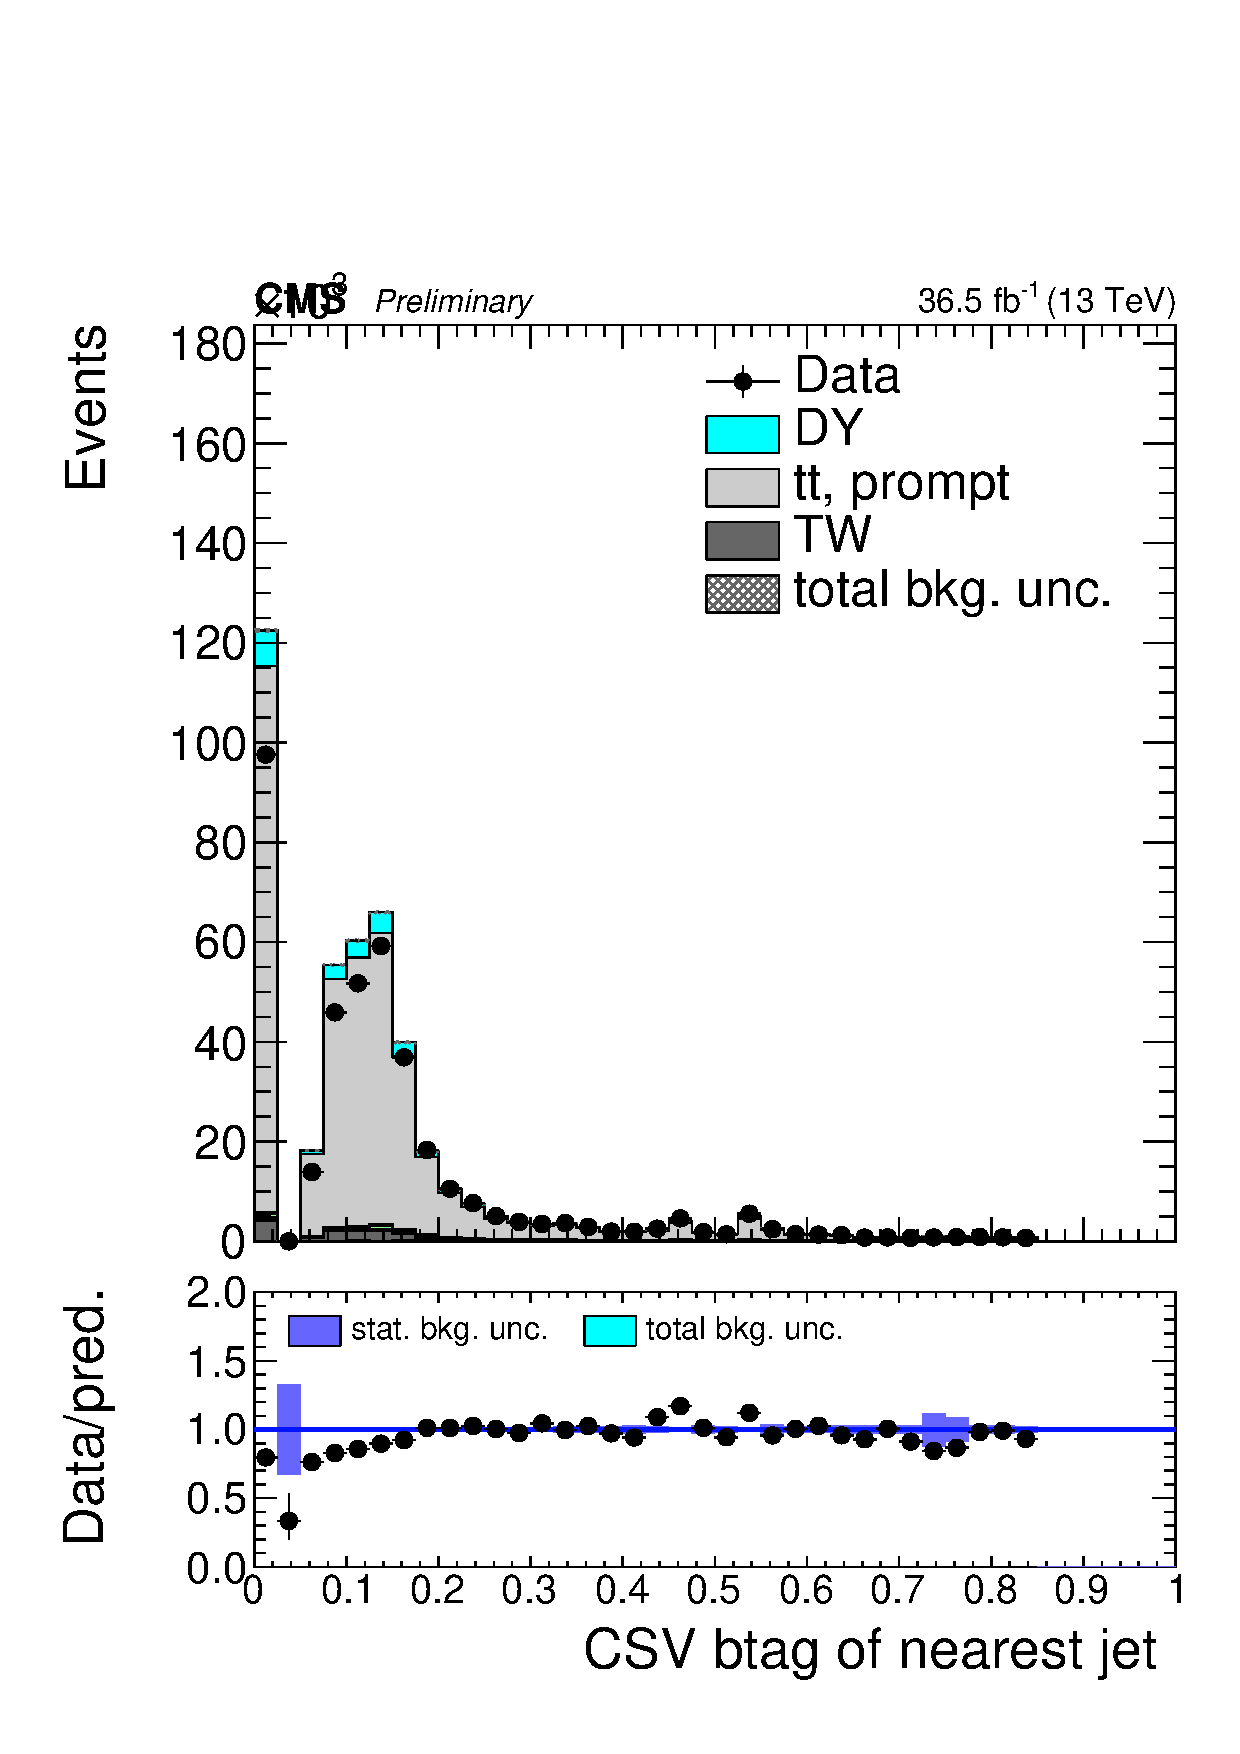
\includegraphics[width=0.32\textwidth]{plots_controlregions/leptons/lep_jetBTagCSV_prompt.pdf}\\
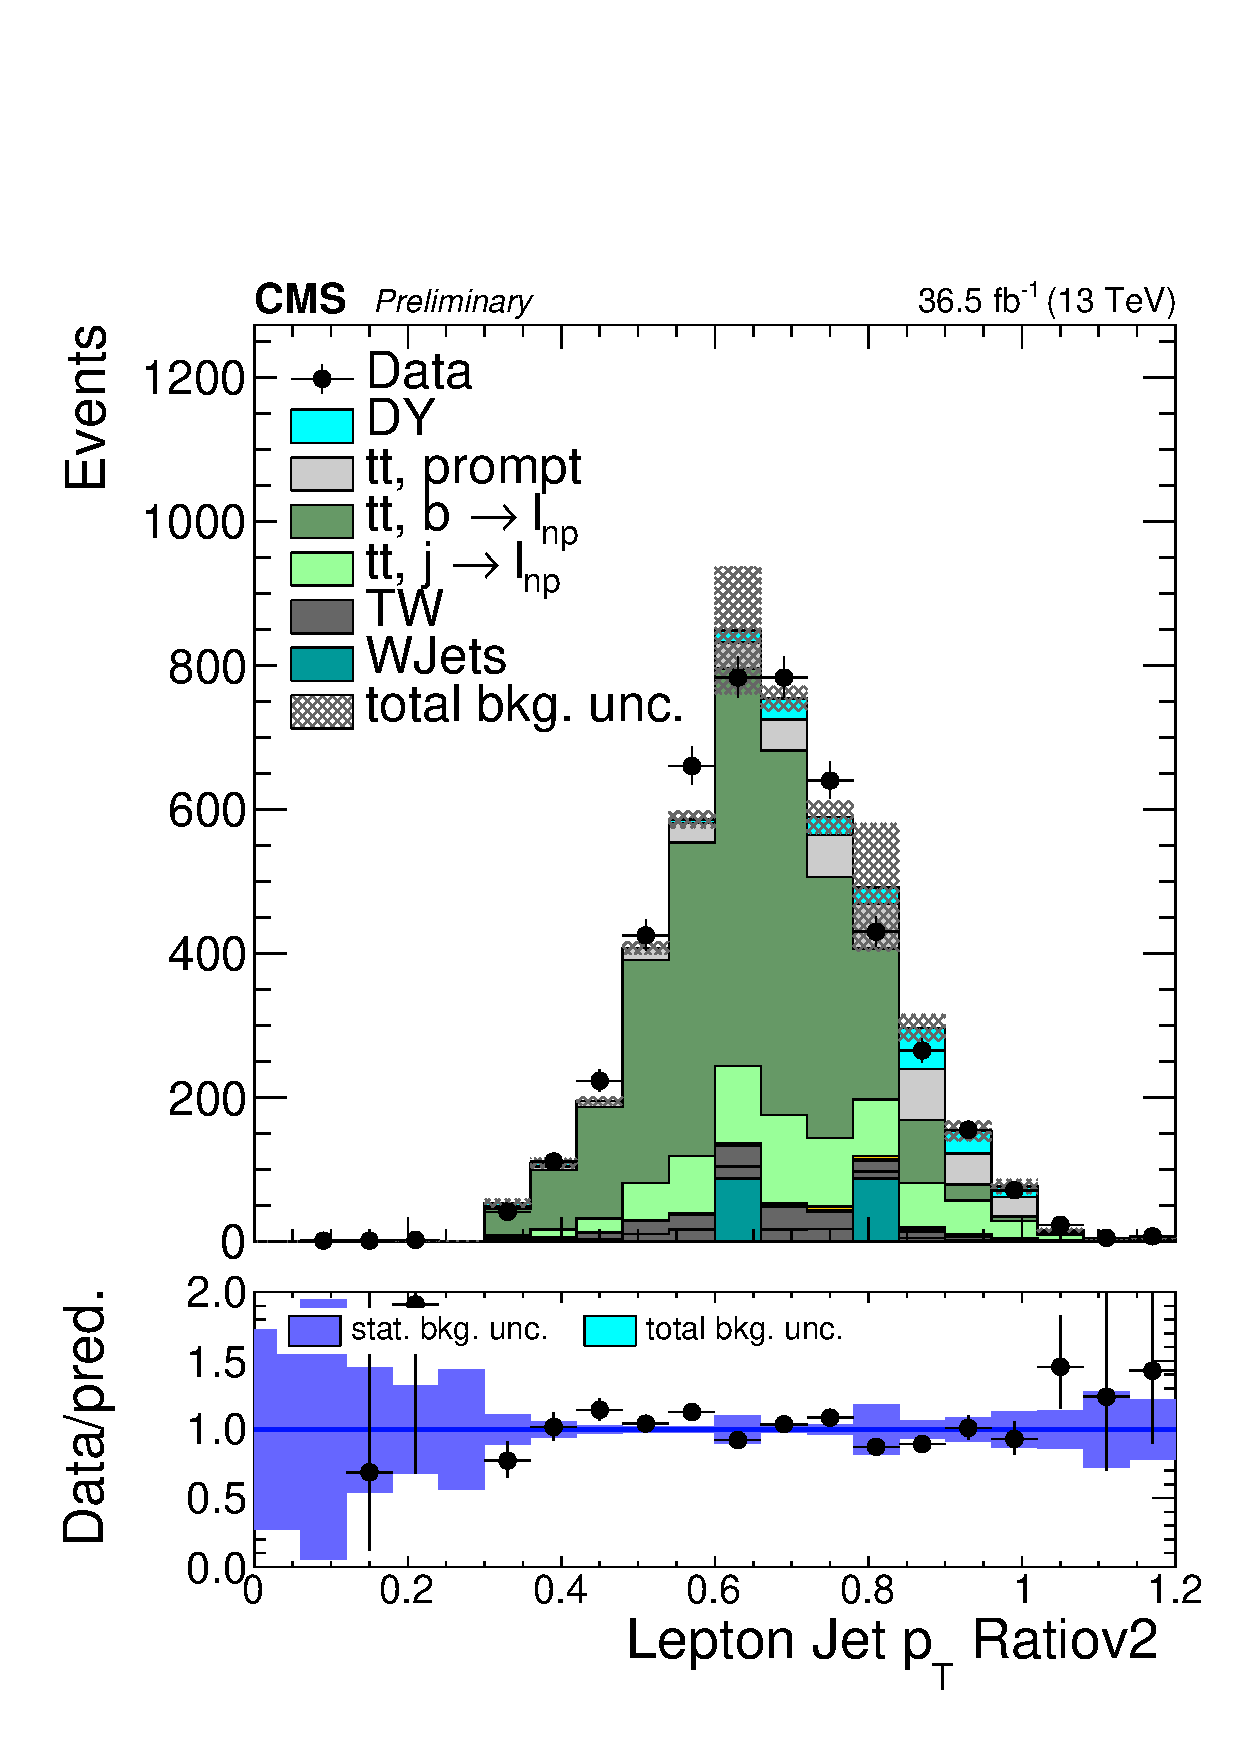
\includegraphics[width=0.32\textwidth]{plots_controlregions/leptons/lep_jetPtRatiov2.pdf}
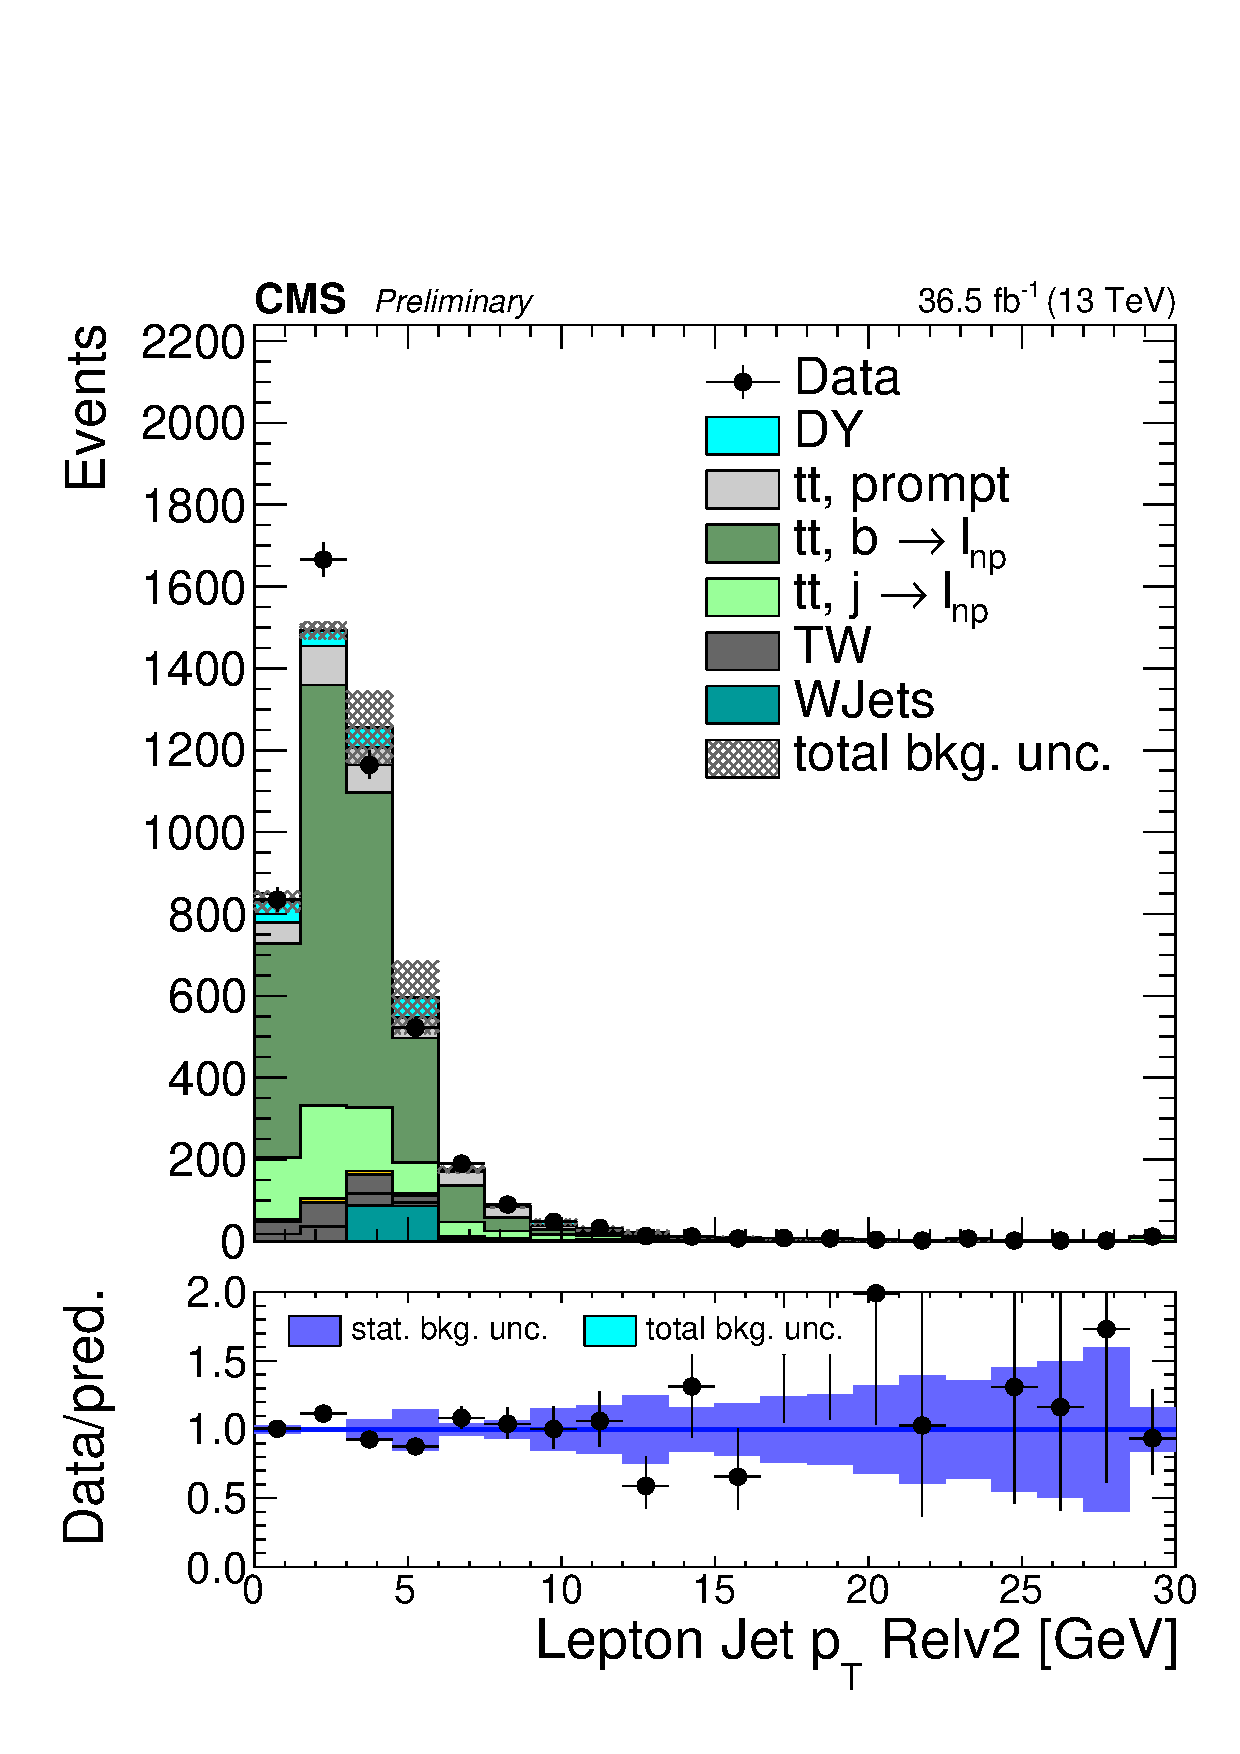
\includegraphics[width=0.32\textwidth]{plots_controlregions/leptons/lep_jetPtRelv2.pdf}
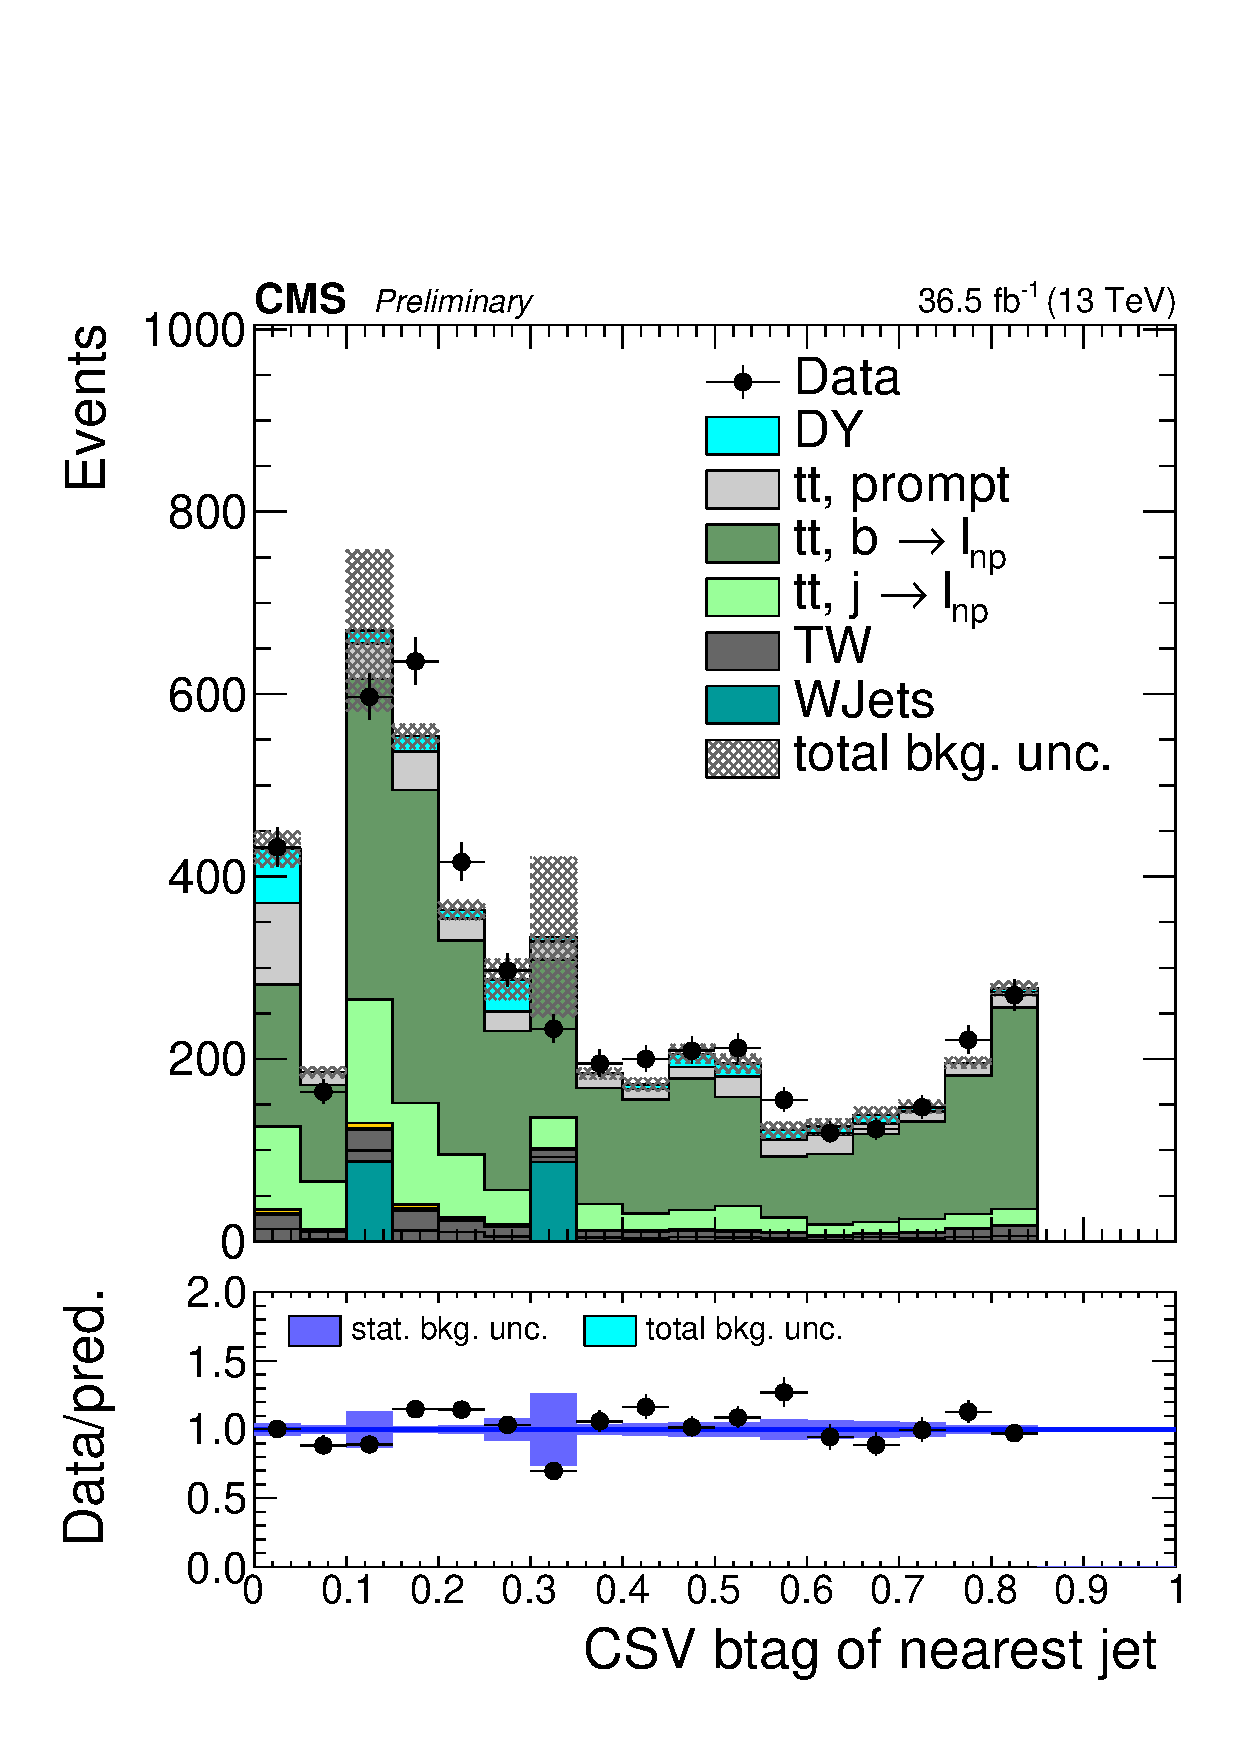
\includegraphics[width=0.32\textwidth]{plots_controlregions/leptons/lep_jetBTagCSV.pdf}\\
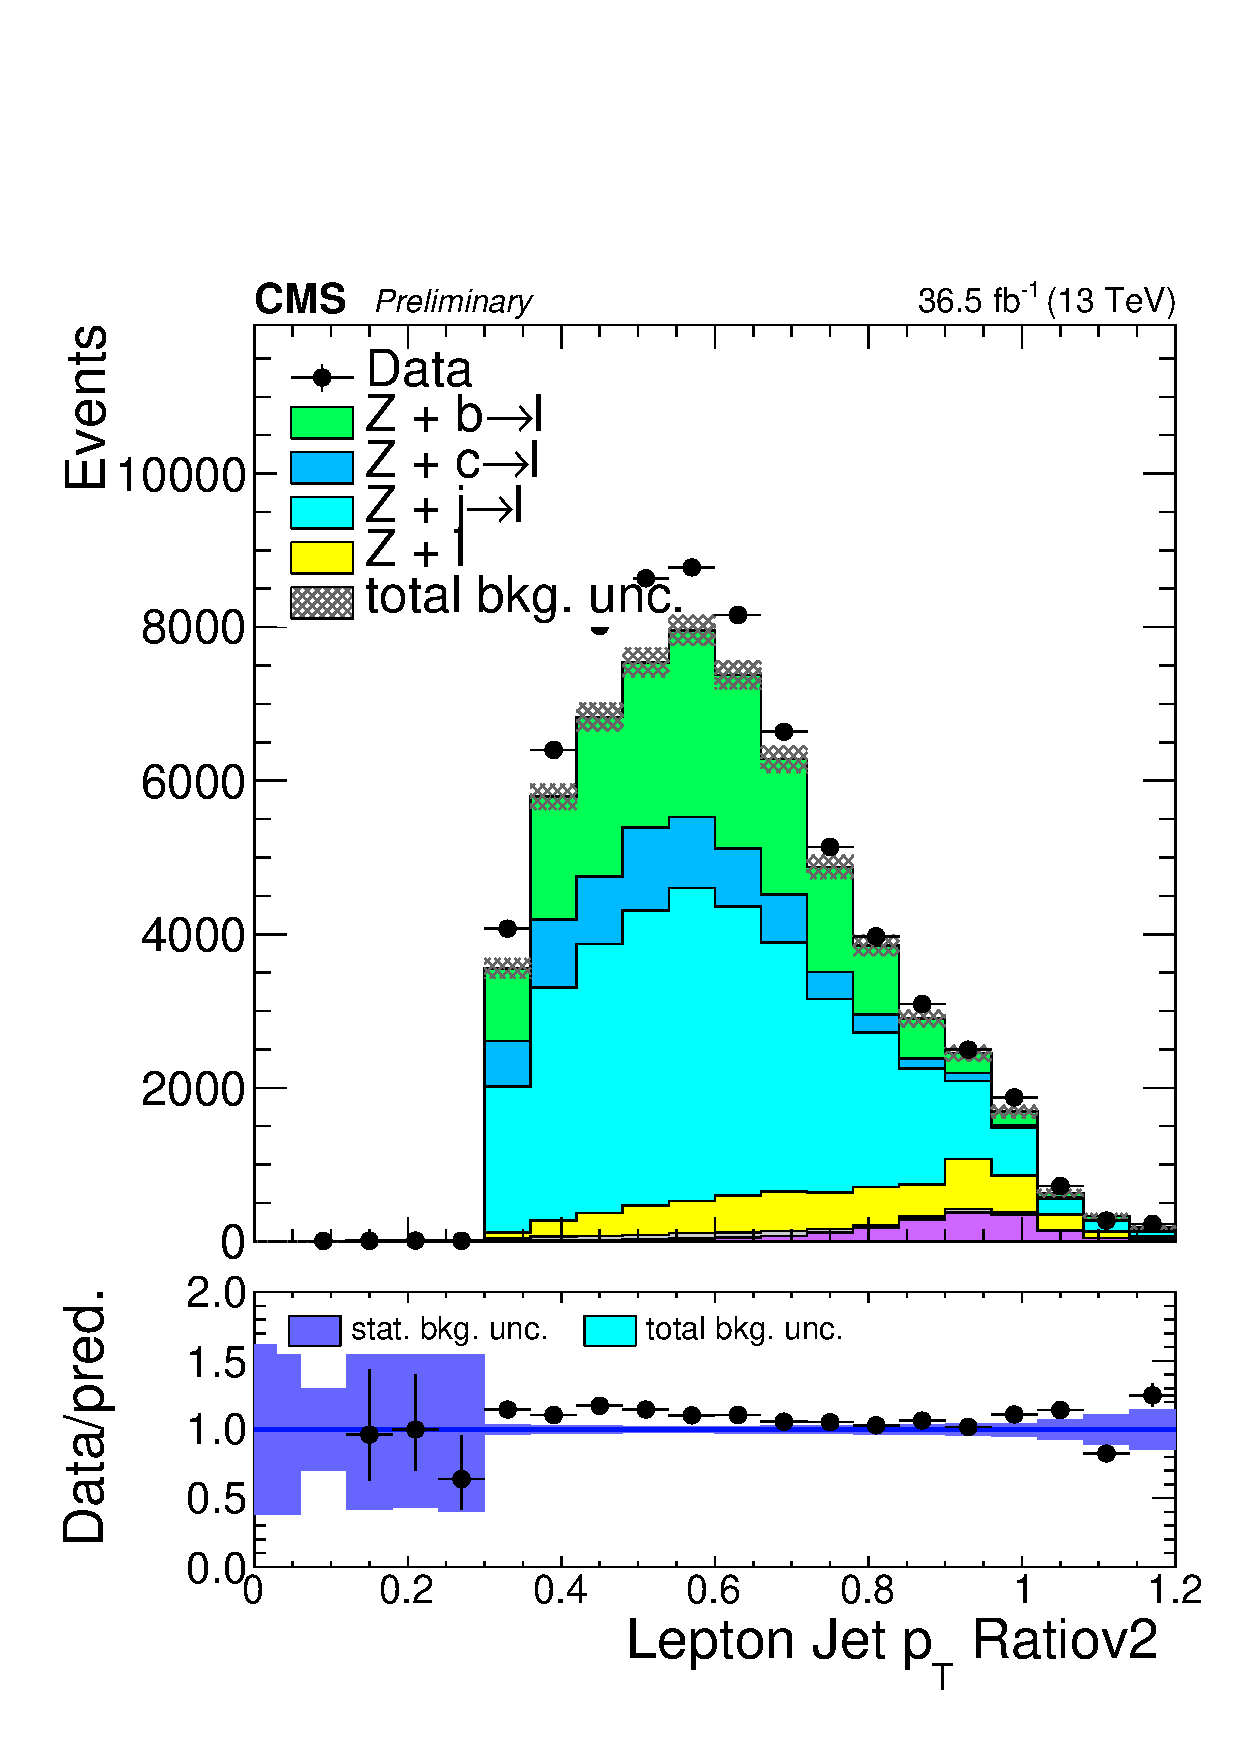
\includegraphics[width=0.32\textwidth]{plots_controlregions/leptons/lep_jetPtRatiov2_Zl.pdf}
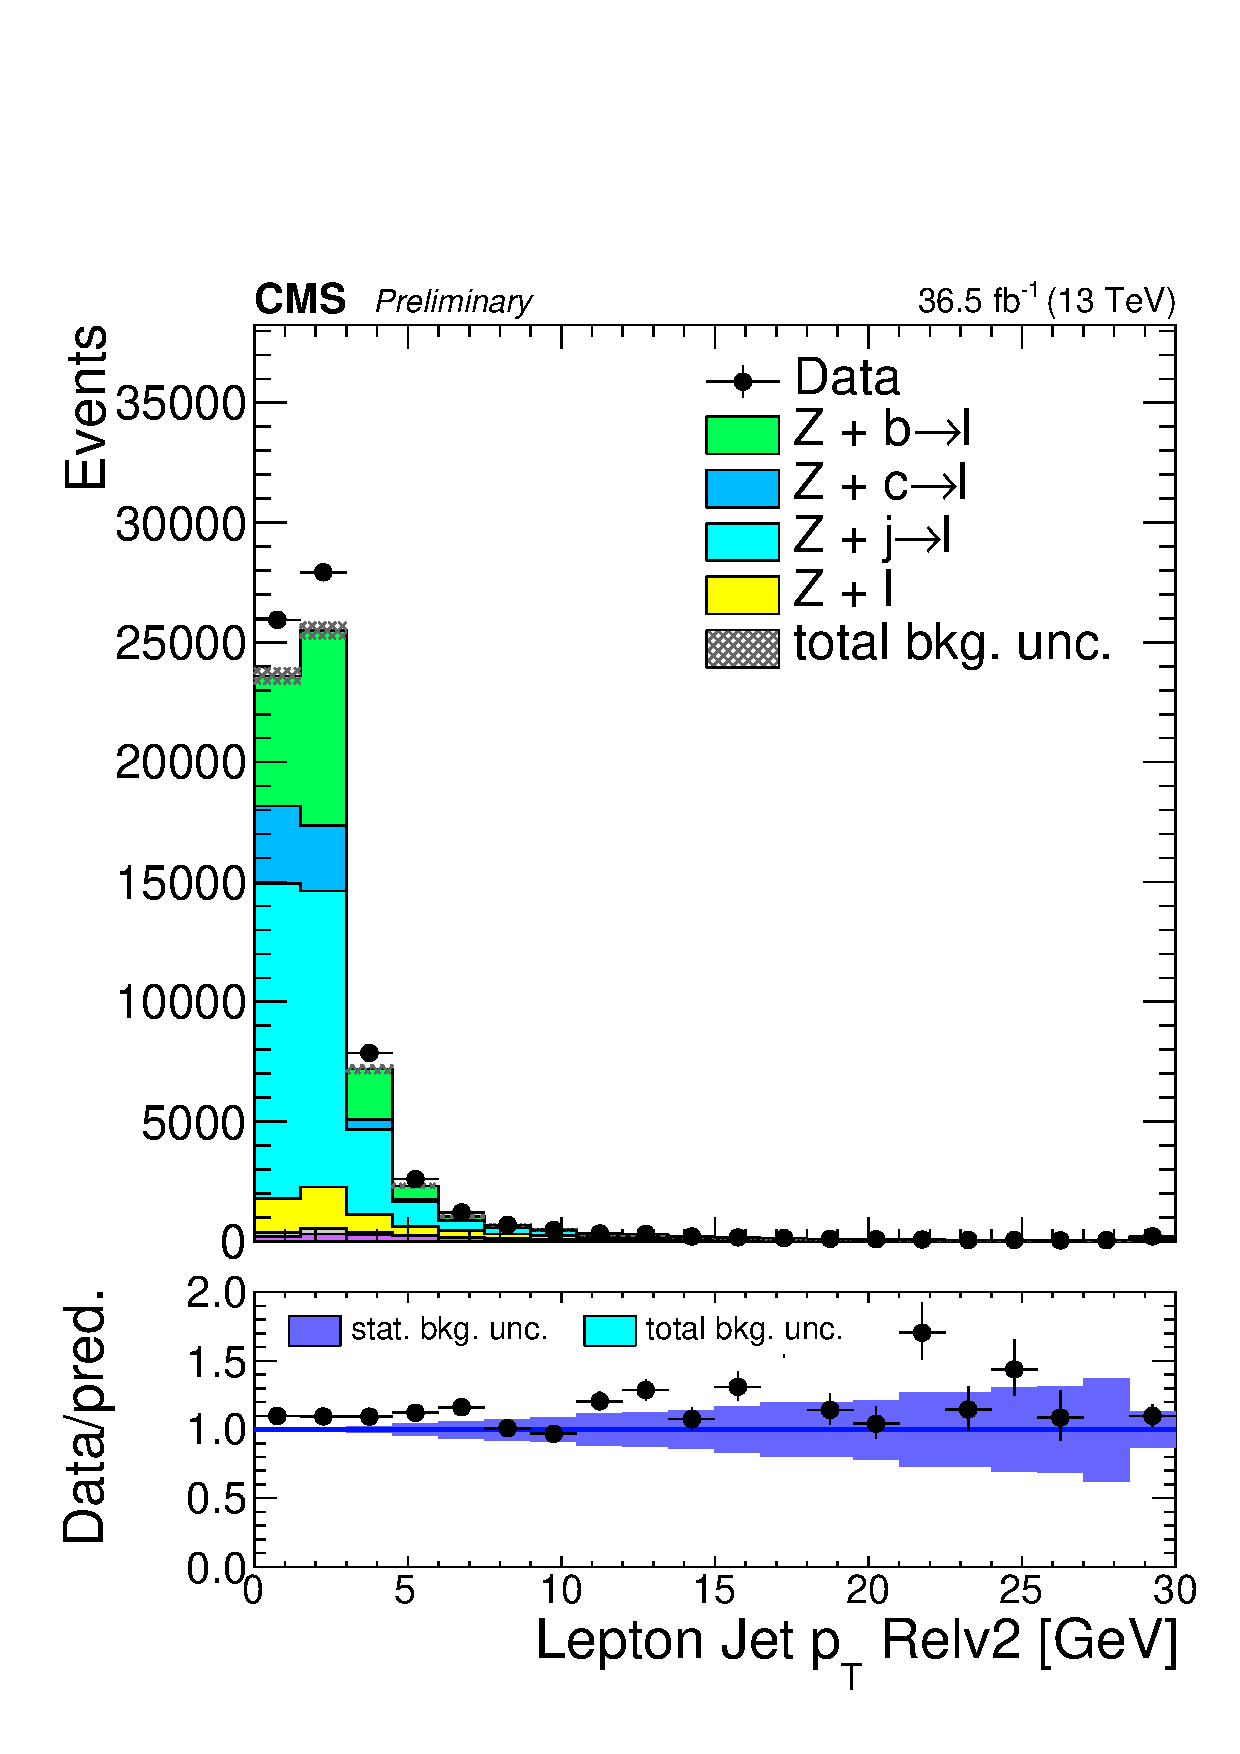
\includegraphics[width=0.32\textwidth]{plots_controlregions/leptons/lep_jetPtRelv2_Zl.pdf}
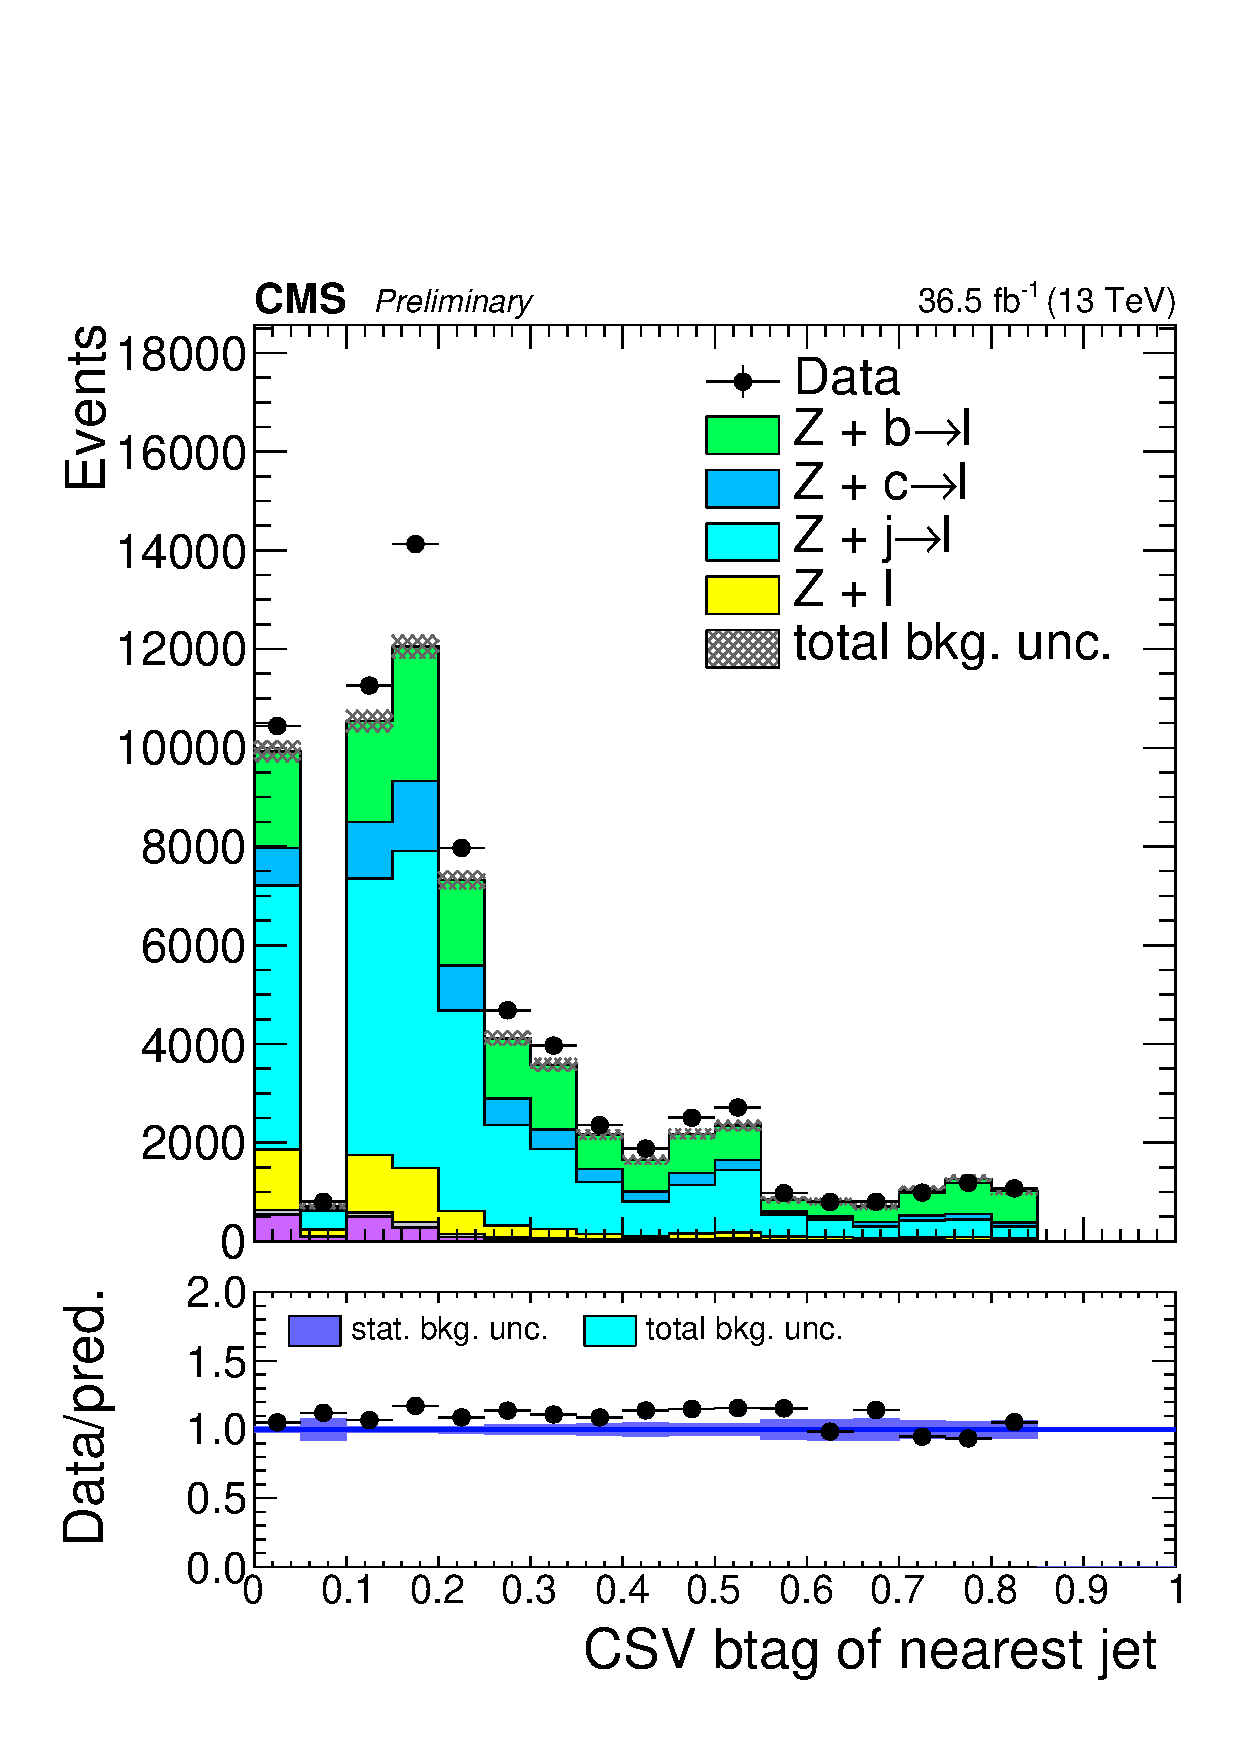
\includegraphics[width=0.32\textwidth]{plots_controlregions/leptons/lep_jetBTagCSV_Zl.pdf}
        \caption{Comparison of the distributions for the lepton $\ptRatio$ (left), $\ptRel$ (center) and the b-tagging discriminator of the associated jet (right),  between data and simulations in control regions enriched in prompt leptons (top), non-prompt leptons (center), and Z+jets events (bottom) , as described in the text. The uncertainty shown on the simulation is only statistical.}
        \label{fig:lep-distributions-2}
\end{figure}

\begin{figure}
        \centering
\includegraphics[width=0.32\textwidth]{plots_controlregions/leptons/ttbar/lep_miniRelIsoCharged_log.pdf}
\includegraphics[width=0.32\textwidth]{plots_controlregions/leptons/ttbar/lep_miniRelIsoNeutral_log.pdf}
\includegraphics[width=0.32\textwidth]{plots_controlregions/leptons/ttbar/lep_sip3d_log.pdf}\\
\includegraphics[width=0.32\textwidth]{plots_controlregions/leptons/ttbar/lep_dxy_log.pdf}
\includegraphics[width=0.32\textwidth]{plots_controlregions/leptons/ttbar/lep_dz_log.pdf}
\includegraphics[width=0.32\textwidth]{plots_controlregions/leptons/ttbar/lep_jetPtRatiov2.pdf}
        \caption{Summary of the input variables to the lepton MVA in a ttbar enriched sample, in data and simulation. The uncertainty shown on the simulation is only statistical.}
        \label{fig:lep-distributions-3}
\end{figure}

\begin{figure}
        \centering
\includegraphics[width=0.32\textwidth]{plots_controlregions/leptons/ttbar/lep_jetPtRelv2.pdf}
\includegraphics[width=0.32\textwidth]{plots_controlregions/leptons/ttbar/lep_jetBTagCSV.pdf}
\includegraphics[width=0.32\textwidth]{plots_controlregions/leptons/ttbar/lep_jetNDauChargedMVASel.pdf}\\
\includegraphics[width=0.32\textwidth]{plots_controlregions/leptons/ttbar/lep_SegmentCompatibility_log.pdf}
\includegraphics[width=0.32\textwidth]{plots_controlregions/leptons/ttbar/el_mvaIdSpring15_log.pdf}
\includegraphics[width=0.32\textwidth]{plots_controlregions/leptons/ttbar/lep_mvaTTH_log.pdf}
        \caption{Summary of the input variables (continued) to the lepton MVA and output discriminator in a ttbar enriched sample, in data and simulation. The uncertainty shown on the simulation is only statistical.}
        \label{fig:lep-distributions-4}
\end{figure}

\newpage
\subsubsection{Loose selection efficiency}\label{sec:looseeff}
The reconstruction and loose identification efficiency are computed
both for muons and electrons using the Tag and Probe technique
with $Z\rightarrow\ell^{+}\ell^{-}$ events, in data and in simulation
separately.
The efficiency scale factor is therefore defined as:
\begin{equation}
  \rho(\pt,\eta) = \frac{\varepsilon_{\rm{data}}(\pt,\eta)}{\varepsilon_{\rm{MC}}(\pt,\eta)},
\end{equation}
where $\varepsilon_{\rm{i}}(\pt,\eta)$ is the efficiency measured for a given lepton in the process i (data or simulation). The scale factor is used afterward to correct the weight of the simulated event.
The full simulation correction from the lepton side is thus given by the product of all scale factors :
\begin{equation}
\rho = \prod_{j \in \rm{leptons}} \rho(\pt(j),\eta_j)
\end{equation}
We apply scale factors for the loose electron selection efficiency that have been derived in the context of the SUSY lepton SF working group.
%In Fig.~\ref{fig:electronTnP} the scale
%factors for the loose electron selection (with the electron
%ID emulation cuts) are shown. 
%Figure~\ref{fig:muonTnP} shows the scale factors for the loose muon
%selection.
The efficiency of tight selection cuts has been measured with the same procedure, with respect to the loose selection.
Systematics on these scale-factors related to the method have been
evaluated and are of the order of 2\% for both lepton flavors, in all
the considered kinematic range.\\

%%% FILL WHEN AVAILABLE
%%% \begin{figure}[!htb]
%%% \centering
%%% \includegraphics[width=0.40\linewidth]{plots_lepEff/TnP_Ele_LooseMVAIDEmuLooseIP.pdf}
%%% \includegraphics[width=0.40\linewidth]{plots_lepEff/TnP_Ele_MiniIsoLoose.pdf} \\
%%% \includegraphics[width=0.40\linewidth]{plots_lepEff/TnP_Ele_ConvMissHits.pdf}
%%% \caption{From left to right: electron data to simulation scale factors for the
%%% Loose WP of the Electron MVA ID together with the Loose IP cuts and
%%% HLT ID Emulation requirements, for the Loose \miniIso, for the Tight
%%% cuts on the conversion veto and the missing inner hits}
%%% \label{fig:electronTnP}
%%% \end{figure}


%\begin{figure}[!hb]
%\centering
%\includegraphics[width=0.30\linewidth]{plots_lepEff/GioEff/mu_ttHPresel_barrel.pdf}
%\includegraphics[width=0.30\linewidth]{plots_lepEff/GioEff/mu_ttHPresel_endcap.pdf}\\
%\includegraphics[width=0.30\linewidth]{plots_lepEff/GioEff/mu_ttHPresel_pt20.pdf}
%\includegraphics[width=0.30\linewidth]{plots_lepEff/GioEff/mu_ttHPresel_pt20_vtx.pdf}
%\caption{From left to right: muon data and simulation efficiency for
%  the preselection (SIP $<$ 8, miniRelIso $<$ 0.4) requirement in the barrel and endcap regions,
%  and muon data and simulation efficiency for the loose impact parameters cuts.}
%\label{fig:muonTnP}
%\end{figure}

\subsubsection{Tight vs Loose selection efficiency}
The efficiencies of applying the tight selection as defined in Tables~\ref{tab:muonIDs} and~\ref{tab:eleIDs}, on the loose leptons are determined using a tag and probe method on a sample of DY-enriched events.
% The denominator definitions for these efficiencies includes the $\text{SIP}_{3D} < 8$ as it is already included in the loose lepton efficiencies described in Section~\ref{sec:looseeff}.
Numerator cuts for the same-sign dilepton efficiencies include the tight-charge requirement.

Number of passed and failed probes are determined from a fit to the invariant mass of the dilepton system.
The resulting efficiencies are shown in Figures~\ref{fig:electronMVAEff_2lss}, \ref{fig:muonMVAEff_2lss}, \ref{fig:electronMVAEff_3l}, and~\ref{fig:muonMVAEff_3l}.

\begin{figure}[!hb]
\centering
  \includegraphics[width=0.31\linewidth]{plots_leptons/lepmva_efficiency/tnp_eff_eb_2lss_pt.pdf}  
  \includegraphics[width=0.31\linewidth]{plots_leptons/lepmva_efficiency/tnp_eff_ee_2lss_pt.pdf}
  %\includegraphics[width=0.31\linewidth]{plots_leptons/lepmva_efficiency/tnp_eff_eb_2lss_nVert.pdf}
\caption{Tight vs loose selection efficiencies for electrons, for the same-sign dilepton lepton definition (\ie\ including the tight-charge requirement).}
\label{fig:electronMVAEff_2lss}
\end{figure}

\begin{figure}[!ht]
\centering
  \includegraphics[width=0.31\linewidth]{plots_leptons/lepmva_efficiency/tnp_eff_mb_2lss_pt.pdf}
  \includegraphics[width=0.31\linewidth]{plots_leptons/lepmva_efficiency/tnp_eff_me_2lss_pt.pdf}
  %\includegraphics[width=0.31\linewidth]{plots_leptons/lepmva_efficiency/tnp_eff_mb_2lss_nVert.pdf}
\caption{Tight vs loose selection efficiencies for muons, for the same-sign dilepton lepton definition (\ie\ including the tight-charge requirement).}
\label{fig:muonMVAEff_2lss}
\end{figure}

\begin{figure}[!ht]
\centering
  \includegraphics[width=0.31\linewidth]{plots_leptons/lepmva_efficiency/tnp_eff_eb_3l_pt.pdf}
  \includegraphics[width=0.31\linewidth]{plots_leptons/lepmva_efficiency/tnp_eff_ee_3l_pt.pdf}
\caption{Tight vs loose selection efficiencies for electrons, for the three lepton channel (\ie\ not including the tight-charge requirement).}
\label{fig:electronMVAEff_3l}
\end{figure}

\begin{figure}[!ht]
\centering
  \includegraphics[width=0.31\linewidth]{plots_leptons/lepmva_efficiency/tnp_eff_mb_3l_pt.pdf}
  \includegraphics[width=0.31\linewidth]{plots_leptons/lepmva_efficiency/tnp_eff_me_3l_pt.pdf}
\caption{Tight vs loose selection efficiencies for muons, for the three lepton channel (\ie\ not including the tight-charge requirement).}
\label{fig:muonMVAEff_3l}
\end{figure}

We use these ($\eta$,$\pt$) dependent scale factors to correct the simulation. 
%A flat uncertainty of 3$\%$ which is of the order of the current statistical uncertainty is assigned to these scale factors. %% FIXME: Update the 3% number?

\subsection{Taus}
\label{subsec:taus}

Hadronically decaying taus ($\tau_h$) are reconstructed using the hadron-plus-strips algorithm \cite{Khachatryan:2015dfa}.
 $\tau_h$ candidates are required to pass the ``decay mode finding'' discriminator, either being reconstruncted in 1- or
 3-prong decay modes with or without additional $\pi^0$'s. In addition, they have to fulfill $p_T>~20~\mathrm{GeV}$ 
and $|\eta|<2.3$, following Tau POG recommandations.

The tau identification criteria applied are based on a tau discriminator, 
using an MVA specifically trained with $t\bar{t}$ and $t\bar{t}H$ events with an isolation cone 
of $\Delta R=0.3$ \cite{AN:MVA_tau_ID_2015}, which increases the efficiency of the tau isolation 
in $t\bar{t}H$ with respect to the default discriminators using an isolation cone of $\Delta R=0.5$. 
The medium working point is used for the tau selection ("byMediumIsolationMVArun2v1DBdR03oldDMwLT").

Reconstructed $\tau_h$ candidates are removed if they overlap within $\Delta R = 0.4$ with \textit{loose} 
electrons or muons. No dedicated discriminators against background from prompt electrons and muons are applied 
since the contribution from background events with additional prompt electrons and muons passing the $\tau_h$ 
selection criteria but not the muon and electron pre-selection requirements is negligible.

In order to ensure orthogonality of our selection from the phase space covered by the 2lss+$\tau_h$, 3l+$\tau_h$ channels,
covered in HIG-17-003, we veto the presence in the event of any $\tau_h$ passing the above selection.


%% flushes all plots before starting
%% next section
\clearpage
\section{Event selection}
\label{sec:selection}
\subsection{Event selection}
Events are selected considering the features of the signal process and the decay signatures.

At least two same-sign or three leptons of any sign, passing the tight selection are required.
In the dilepton channels, events are vetoed if they contain additional tight leptons.

Events are required to have fired one of the corresponding trigger paths, and are vetoed if any loose lepton pair has an invariant mass below $12\GeV$.

In the dilepton channels, the leptons are required to have $\pt>25\GeV$ for the leading, and $\pt>15\GeV$ for the sub-leading lepton.
In the three lepton channel, they are required to have respectively $\pt>25\GeV$, $>15\GeV$, and $>15\GeV$.

Three lepton events with an opposite-sign, same-flavor lepton combination with invariant mass within 15\GeV\ of the \Z\ boson mass are discarded to reject events from \WZ+jets production.
Same-sign di-electron events where the two electrons have invariant mass within 10\GeV\ of the \Z\ boson mass are equally discarded to reject events from DY+jets production with charge mis-identified electrons.

Leptons in the three lepton channel are not required to pass the triple charge consistency criteria (for electrons), or the $\Delta{\pt}/\pt <0.2$ cut (for muons).

Furthermore we require at least two jets of which at least one passes the medium \cPqb\ tagging working point ($\pt>25\GeV$ and $|\eta|<2.4$), and at least one not passing the loose working point ($\pt>25\GeV$ for $|\eta|<2.4$ and $\pt>40\GeV$ for $|\eta|>2.4$).

The event selection is summarized in Tab~\ref{tab:evsel}.

\begin{table}[h!]
\centering
\begin{tabular}{c|c}
	\hline
	\multicolumn{2}{c}{No loose leptons with $m_{\ell\ell} < 12\GeV$} \\
	%\multicolumn{2}{c}{Two or more jets with $\pt>25\GeV$} \\
	\multicolumn{2}{c}{One or more jets passing CSV medium ($|\eta|<2.4$)} \\
	\multicolumn{2}{c}{One or more jets failing CSV loose} \\
	\hline
	Exactly two tight same-sign leptons & Exactly three tight leptons \\
	$\pt>25/15\GeV$ & $\pt>25/15/15\GeV$ \\
	No \Pe\Pe\ events with $|m_{\Pe\Pe}-m_\Z|<10\GeV$ & No OSSF pair with $|m_{\ell\ell}-m_\Z|<15\GeV$ \\
	Triple charge consistent electrons &  \\
	Muons with $\Delta{\pt}/\pt <0.2$ &  \\
	\hline
\end{tabular}
\caption{Summary of event selection.}\label{tab:evsel}
\end{table}

\begin{table}[thb]
\centering
\begin{tabular}{lrrrr}
\multicolumn{1}{c@{\qquad}}{} &
\multicolumn{1}{c@{\qquad}}{$3\ell$} &
\multicolumn{1}{c}{$\Pgm\Pgm$} &
\multicolumn{1}{c@{\qquad}}{$\Pe\Pgm$} &
\multicolumn{1}{c}{$\Pe\Pe$} \\ \hline
$\ttW$                        & $  22.50 \pm 0.35$ & $ 68.03 \pm 0.61 $ & $ 97.00 \pm 0.71 $ & $ 29.63 \pm  0.39 $ \\
$\ttZ\!/\!\gamma^*$           & $  32.80 \pm 1.79$ & $ 25.89 \pm 1.12 $ & $ 64.82 \pm 2.42 $ & $ 28.74 \pm  1.70 $ \\
$\WZ$                         & $   8.22 \pm 0.86$ & $ 15.07 \pm 1.19 $ & $ 26.25 \pm 1.57 $ & $  9.31 \pm  0.93 $ \\
$\ZZ$                         & $   1.62 \pm 0.33$ & $  1.16 \pm 0.29 $ & $  2.86 \pm 0.45 $ & $  1.09 \pm  0.27 $ \\
$\PW^\pm\PW^\pm\cPq\cPq$      & --                 & $  3.96 \pm 0.52 $ & $  6.99 \pm 0.69 $ & $  2.19 \pm  0.37 $ \\
$\PW^\pm\PW^\pm \text{(DPS)}$ & --                 & $  2.48 \pm 0.42 $ & $  4.17 \pm 0.54 $ & $  0.81 \pm  0.24 $ \\
VVV                           & $   0.42 \pm 0.16$ & $  2.99 \pm 0.34 $ & $  4.85 \pm 0.43 $ & $  1.19 \pm  0.21 $ \\
$\mathrm{tttt}$               & $   1.84 \pm 0.44$ & $  2.32 \pm 0.45 $ & $  4.06 \pm 0.57 $ & $  0.89 \pm  0.31 $ \\
$\mathrm{tZq}$                & $   3.92 \pm 1.48$ & $  5.77 \pm 2.24 $ & $ 10.73 \pm 3.03 $ & $  7.56 \pm  1.72 $ \\
$\mathrm{tZW}$                & $   1.70 \pm 0.12$ & $  2.13 \pm 0.13 $ & $  3.91 \pm 0.18 $ & $  1.13 \pm  0.10 $ \\
$\gamma$ conversions          & $   7.43 \pm 1.94$ & --                 & $ 23.81 \pm 6.04 $ & $  9.87 \pm  4.17 $ \\ \hline
Non-prompt                    & $  25.61 \pm 1.26$ & $ 80.94 \pm 2.02 $ & $135.34 \pm 2.83 $ & $ 47.72 \pm  1.79 $ \\
Charge mis-ID                 & --                 & --                 & $ 58.50 \pm 0.31 $ & $ 44.52 \pm  0.31 $ \\ \hline
All backgrounds               & $ 106.05 \pm 3.45$ & $210.74 \pm 3.61 $ & $443.30 \pm 8.01 $ & $184.65 \pm  5.29 $ \\ \hline
$\tHq$ ($\Ct=-1.0$)           & $   7.48 \pm 0.14$ & $ 18.48 \pm 0.22 $ & $ 27.41 \pm 0.27 $ & $  8.47 \pm  0.15 $ \\
$\tHW$ ($\CV=-1.0$)           & $   7.38 \pm 0.16$ & $  7.72 \pm 0.17 $ & $ 11.23 \pm 0.20 $ & $  3.66 \pm  0.11 $ \\
$\ttH$                        & $  18.29 \pm 0.41$ & $ 24.18 \pm 0.48 $ & $ 35.21 \pm 0.58 $ & $ 11.07 \pm  0.32 $ \\ \hline
Data (35.9\fbinv)             & \multicolumn{1}{l}{149}&\multicolumn{1}{l}{280} & \multicolumn{1}{l}{525} & \multicolumn{1}{l}{208}               \\
\end{tabular}
\caption{Expected and observed yields for $35.9\fbinv$ after the selection in all final states. Uncertainties are statistical only.}
\label{tab:yields-sel}
\end{table}

In the multi-leptonic final states of the signal processes, the largest contribution is from Higgs decays to $\PW\PW$, $\sim 75\%$ of the time, as shown in Tab~\ref{tab:yield_hbr}.
This is followed by the $\tau \tau$ and $ZZ$ decay modes respectively.
A minor contribution is also there from Higgs to $\mu \mu$ and $\gamma \gamma$ decays.

\begin{table}[HBR]
\centering
\begin{tabular}{lrrrr}
\multicolumn{1}{c@{\qquad}}{} &
\multicolumn{2}{c@{\qquad}}{$3\ell$} &
\multicolumn{2}{c}{$\Pgm\Pgm$} \\ \hline
$\tHq (\mathrm{Inclusive})$  & $\mathbf{6.57}$ & 100.0\% & $\mathbf{17.38}$ & 100.0\% \\
$\tHq (\PH\to \PW\PW)$       & $4.84$  & 73.9\%   & $13.33 $ &  76.9\%  \\
$\tHq (\PH\to \tau\tau)$     & $1.04$  & 15.9\%   & $ 3.62 $ &  20.6\%  \\
$\tHq (\PH\to \Z\Z)$         & $0.48$  &  7.2\%   & $ 0.37 $ &   2.2\%  \\
$\tHq (\PH\to \mu\mu)$       & $0.21$  &  3.0\%   & $ 0.04 $ &   0.2\%  \\
$\tHq (\PH\to \gamma\gamma)$ & $<0.01$ &  0.1\%   & $ 0.02 $ &   0.1\%  \\
$\tHq (\PH\to \cPqb\cPqb)$   & $<0.01$ & $<0.1$\% & $ 0.01 $ & $<0.1$\% \\ \hline
$\tHW (\mathrm{Inclusive})$  & $\mathbf{7.32}$ & 100.0\% & $\mathbf{7.62}$ & 100.0\% \\
$\tHW (\PH\to \PW\PW)$       & $5.50 $ &  76.9\%  & $ 5.60$ & 74.1\% \\
$\tHW (\PH\to \tau\tau)$     & $1.40 $ &  20.6\%  & $ 1.81$ & 23.1\% \\
$\tHW (\PH\to \Z\Z)$         & $0.31 $ &   2.2\%  & $ 0.21$ &  2.7\% \\
$\tHW (\PH\to \mu\mu)$       & $0.12 $ &   0.2\%  & $ 0.01$ &  0.1\% \\
$\tHW (\PH\to \gamma\gamma)$ & $<0.01$ & $<0.1$\% & $<0.01$ &$<0.1$\% \\
$\tHW (\PH\to \cPqb\cPqb)$   & $<0.01$ & $<0.1$\% & $<0.01$ &$<0.1$\% \\ \hline
\end{tabular}
\caption{Signal yields split by decay channels of the Higgs boson. (Note that these numbers are with a forward jet $\pt$ cut at 25\GeV.)}
\label{tab:yield_hbr}
\end{table}



\section{Signal extraction}
\label{sec:extraction}
Despite the event selection requirements previously described, the post-selection yields are still dominated by the backgrounds,
and have insufficient statistics to determine the presence of the ttH signal, making further discrimination necessary.
The approach adopted in this search is to split the selected events into several mutually exclusive categories with
different signal to background ratios.
In each of these categories the signal is extracted from the distribution of a suitable discriminating variable.

In order to exploit the topological characteristics and specificities of the ttH signal with respect to the most
dominant backgrounds, the output of the boosted decision tree (BDT), trained using a selection of kinematic
variables, is used as the discriminating variable for the signal extraction.
In this analysis, the samples used for BDT training and evaluation are the ones reported in Sec. \ref{sec:samples}.

Both final states with two same sign leptons (2lss) and at least three leptons ($\geq$=3l) have dominant backgrounds originating
from the \ttbar\ and \ttV\ (V=W/Z) processes. In order to have an efficient discrimination against both of these processes,
a two-dimensional (2D) BDT approach is introduced. For each of the 2lss and $\geq$=3l final states, the BDT is separately trained
against the \ttbar\ and \ttV, selecting a set of kinematic variables that provide the largest separation in each training. The BDT
outputs of the training against these two processes are used to construct the 2D space, effectively a scatter plot of the
two discriminators. The consequent 2D distribution is then partitioned to rectangular sectors and ttH signal and background contributions
of each sector are summed and folded to a one-dimensional histogram. With a
convenient partitioning of the 2D space, the resulting difference of the signal and background shapes is enhanced with respect to the
one-dimensional case, for example against the \ttbar, and that is provided by the training of the additional BDT, against the \ttV\  process.

In the following subsections we detail the definitions of the BDTs used as discriminating variable for the signal extraction
in the 2lss and $\geq$=3l categories. We then describe the criterion to decide the binning of the 2D BDT.
Finally, we detail the precise event subcategorization.

\subsection{2lss event BDT}\label{sec:2lss event BDT}
The training is performed using a relaxed event selection that requires at least two preselected same sign leptons with leading and trailing lepton transverse momentum larger than 25 and 15 GeV, respectively, plus at least four jets in the event of which either two loose selected b-jets or one medium b-tagged jet.

The training against the \ttbar background is performed considering the following input variables:
\begin{itemize}
\item maximum absolute pseudorapidity of the two leading leptons
\item multiplicity of hadronic jets
\item minimum distance between the leading lepton and closest jet
\item minimum distance of the trailing lepton and closest jet
%\item missing transverse energy
%\item average separation between the two jets and the transverse mass of the leading lepton 
\item transverse mass of the leading lepton and missing transverse energy
\item hadronic top reconstruction (score of the discriminator for best permutation)
\end{itemize}

The training against the \ttV\  background is performed considering the following input variables:
\begin{itemize}
\item maximum absolute pseudorapidity of the two leading leptons
\item multiplicity of hadronic jets
\item minimum distance between the leading lepton and closest jet
\item minimum distance of the trailing lepton and closest jet
\item transverse mass of the leading lepton and missing transverse energy
\item leading lepton transverse momentum 
\item trailing lepton transverse momentum
%\item HT, defined as the scalar sum of the pT of the selected leptons, jets, and the met
\item Hj tagger score after hadronic top jets triplet removal (best permutation)
%\item Hj and Hjj taggers after hadronic top jets triplet removal
\end{itemize}

%The variables listed above are the same used in the previous versions of the analyses,
%with the exception of HT, which is now used in the training against \ttV\, and the last-itemized for both trainings.
The sets of observables listed above include new variables that have not been used before, such as the 
score of the hadronic top reconstruction and the Hj tagger, which are explained in more detail below.
The aforementioned hadronic top jet triplet, when using the Hj tagger in the training against the \ttV\ background,
indicates a triplet of jets with the highest likelihood to orginate from hadronic top decay in 2lss events.
This jet triplet is found through the event reconstruction BDT explained below, whose score is used as an input in the training against \ttbar.
The Hj tagger, described more in detail in the following,
is an algorithms designed to identify jets originating from one of the W of the Higgs in 2lss events.
The Higgs jets search is performed against all the jets that enter the 2lss region, except those forming a triplet compatible
with an hadronic top decay (from which the expression hadronic top jets triplet removal).

\subsubsection{Hadronic top reconstruction}
The reconstruction of the hadronic top decay is performed with a BDT. The objective is to correctly match
each selected jet and lepton to a final state particle in a $t\bar{t}H$ event, then
use the BDT response and other variables from the reconstruction to discriminate
against events without a hadronic top.     

Event reconstruction targets the 2lss category, specifically where the Higgs decays
to $W$ bosons. In the 2lss category, this means that one lepton originates from the
top system, and the other from the Higgs. For the jets, one of the
$W$ bosons from the Higgs decays hadronically, one of the top quarks decays
hadronically, producing a total of two b-jets, and four light-flavor jets
from the hadronic $W$ decays.   

{\bfseries Training}

The event reconstruction BDT is trained using the $t\bar{t}H$ monte-carlo powheg
signal sample described previously. 

The signal is correctly matched $t\bar{t}H$ events, which pass the 2lss selection.
Because the 2lss event selection requires at least four jets, the vast majority of signal
events used for training are only partially reconstructed, since a full reconstruction
necessitates six matched jets. Because so few events can be fully reconstructed, we must
consider partial reconstructions for events that have fewer than six matched jets.
The strategy for this is to use 'null' jets whose four-vectors are set to zero to
substitute missing jets in the event. Finally we require the signal events to have two
correctly matched selected leptons, and at least four correctly matched selected jets.

The background consists of all jet and lepton permutations of incorrectly matched
$t\bar{t}$ events. For the background, the null jets are added according to the
jet multiiplicity. For events with seven or fewer selected jets, three null jets are
added, for events with eight selected jets, two null jets are added, and one null jet
is added for events with greater than eight selected jets. To reduce the computation
time and improve performance,
several cuts are applied at each permutation to remove unlikely reconstructions.
These cuts include applying the b-tag requirement on the two jets being considered
as b-jets (1 b-tight, 2 b-loose) described earlier, requiring that no
reconstructed $W$ have a mass greater than 120 GeV, requiring the leptonic top mass
be less than 180 GeV, and requiring 
the hadronic top mass be less than 220 GeV. Additionally, we ignore permutations
arising from swapping two light flavor jets from the same $W$ boson, as the reconstruction is
identical. 

The BDT uses eight input variables, consisting of the CSV of the b-jets from the top
system, the transverse
momentum of the reconstructed hadronic top, the mass of the reconstructed hadronic top,
the mass of the $W$ originating from the hadronic top, the transverse momentum ratio
of lepton from the Higgs with the lepton from the top, and the solid angles between
the lepton from the top and
each b-jet from the top system, and between the lepton from the Higgs.
This approach focuses on the hadronic top decay, as the other aspects of the event
are more difficult to reconstruct due to the missing energy from the neutrinos. 

{\bfseries Evaluation}

The event reconstruction BDT is evaluated by iterating over all possible lepton and jet
permutations, and selecting the highest scoring permutation as the reconstruction for
each event. For the evaluation and usage, the null jet prescription and permutation
cuts used are identical to the background training.
The reconstruction is designed identify events that have a hadronic top present and thus offers
some discrimination against the semi-leptonic $t\bar{t}$ background, shown below in
Figure~\ref{reconstruction:outputVars}.


\begin{figure}[htb]
 \centering
   \includegraphics[width=0.4\textwidth]{plots_reconstruction/had_top_mass.png}
   \includegraphics[width=0.4\textwidth]{plots_reconstruction/had_top_pt.png}\\
   \includegraphics[width=0.4\textwidth]{plots_reconstruction/bdt_score.png}
   \caption{Best BDT score and associated quantities from hadronic top reconstruction.}
  \label{reconstruction:outputVars}
\end{figure}

%% \begin{figure}[htb]
%%  \centering
%%    \includegraphics[width=0.7\textwidth]{plots_reconstruction/roc_improvement.png}
%%    \caption{ROC curve of signal extraction BDT with and without reconstruction variables evaluated against $t\bar{t}$.}
%%   \label{reconstruction:roc}
%% \end{figure}


%% \begin{figure}[htb]
%%  \centering
%%    \includegraphics[width=0.7\textwidth]{plots_reconstruction/reconstruction_mva_csv_signal_region.png}
%%    \includegraphics[width=0.7\textwidth]{plots_reconstruction/reconstruction_topmass_toppt_signal_region.png}
%%    \caption{Event reconstruction variables in the 2lss signal region.}
%%   \label{reconstruction:vars_signal_region}
%% \end{figure}

%% \begin{figure}[htb]
%%  \centering
%%    \includegraphics[width=0.7\textwidth]{plots_reconstruction/reconstruction_mva_csv_application_region.png}
%%    \includegraphics[width=0.7\textwidth]{plots_reconstruction/reconstruction_topmass_toppt_application_region.png}
%%    \caption{Event reconstruction variables in the 2lss application region.}
%%   \label{reconstruction:vars_application_region}
%% \end{figure}

%% \begin{figure}[htb]
%%  \centering
%%    \includegraphics[width=0.7\textwidth]{plots_reconstruction/reconstruction_extraction_mva_output.png}
%%    \caption{Signal extraction MVA output with and with out signal extraction.}
%%   \label{reconstruction:extraction_output}
%% \end{figure}

\clearpage
\subsubsection{The Hj tagger}\label{sec:Hjtagger}
In this section we describe a discriminator aiming at identifying jets that originates from a Higgs decaying to two Ws.
In particular, we target the 2lss category in which the ttH signal decays, in the highest fraction of events, according to the following chain:
$$(t) (t) (H) \rightarrow  (bW) (bW) (WW^*) \rightarrow (bjj)  (b\ell\nu_{\ell}) (\ell\nu_{\ell}jj)$$
We therefore expect 2 b quark jets, 4 jets, 2 same-sign leptons, and missing energy in the final state,
altough, in order to increase the signal acceptance, the analysis requires the presence of at least 4 jets overall.
This means that the Higgs jets do not necessarily enter the signal region.

In order to deal with both the complicated jet combinatoric and the possibility that not all the jets originating from Higgs are selected,
one discriminator is developed: the Higgs-jet (Hj) tagger.
The Hj tagger is an object discriminator that exploits jet identification and kinematic properties
in order to assess the likelihood of a jet of originating in the decay $H \rightarrow WW^* \rightarrow \ell\nu_{\ell}jj$.

The discriminator is developed considering the BDT  multivariate technique.
We rely on the powheg ttH sample and ttV sample to define the signal and the background in the training.
For the Hj tagger the signal is represented by reconstructed jets that are matched at gen-level to jets
of the process $H \rightarrow WW^* \rightarrow \ell\nu_{\ell}jj$, while the background is given by the reconstructed jets in ttV events. 
For the training, we consider the phase space of events that enter the 2lss category, with 0 $\tau_h$.

In the following subsection we list the variables used for the Hj taggers and their expected BDT distributions.

{\bfseries Hj variables and performances}\\
The variables used for the Hj tagger are:
\begin{itemize}
\item minimum dR of the jet and one of the lepton
\item maximum dR of the jet and one of the lepton
\item jet pT
\item jet b-tagging discriminator
\item jet quark-gluon discriminator
\end{itemize}

The performances of the Hj tagger are illustrated in Fig. \ref{fig:HjDistrROC}.
The ROC curve (Fig. \ref{fig:HjDistrROC}, right) highlights the improvement
in performance of the Moriond 2017 BDT (red line) versus the ICHEP 2016 BDT (black line).

\begin{figure}[htb]
 \centering
   \includegraphics[width=0.48\textwidth]{plots_HjHjj/Jtagger_Ks_.png}
   \includegraphics[width=0.48\textwidth]{plots_HjHjj/Roc_Comparison_18Feb.pdf}
   \caption{The Hj distribution (left) and ROC (right). The ROC curve highlights the improvement in performance of the Moriond 2017 BDT (red line) versus            the ICHEP 2016 BDT (black line). Signal and background composition are described in the text.}
   %\caption{The Hj ROC. Signal and background composition are described in the text.}
  \label{fig:HjDistrROC}
\end{figure}

Figures~\ref{fig:2lss_training_1} and \ref{fig:2lss_training_2} show a comparison of the simulated signal (ttH) and background (\ttbar\ or \ttV) processes for each of the input variables to the BDT discriminator.
Figure ~\ref{fig:2l_mvaTraining} shows the separation power of the BDT discriminators.
%while Figures~\ref{fig:2l_mvaOutput} shows the distributions of these discriminators.

\begin{figure}[htb]
        \centering
\includegraphics[width=0.32\textwidth]{plots_extraction/training/2lss/kinMVA_input_max_Lep_eta.pdf}
\includegraphics[width=0.32\textwidth]{plots_extraction/training/2lss/kinMVA_input_numJets.pdf}\\
\includegraphics[width=0.32\textwidth]{plots_extraction/training/2lss/kinMVA_input_mindr_lep1_jet.pdf}
\includegraphics[width=0.32\textwidth]{plots_extraction/training/2lss/kinMVA_input_mindr_lep2_jet.pdf}
%\includegraphics[width=0.32\textwidth]{plots_extraction/training/2lss/kinMVA_input_met.pdf}
%\includegraphics[width=0.32\textwidth]{plots_extraction/training/2lss/kinMVA_input_avg_dr_jet.pdf}
        \caption{The separation power of the variables used for BDT trainings, in the two same sign leptons channel.}
        \label{fig:2lss_training_1}
\end{figure}

\begin{figure}[htb]
        \centering
\includegraphics[width=0.32\textwidth]{plots_extraction/training/2lss/kinMVA_input_MT_met_lep1.pdf}
\includegraphics[width=0.32\textwidth]{plots_extraction/training/2lss/kinMVA_input_LepGood0_conePt.pdf}\\
\includegraphics[width=0.32\textwidth]{plots_extraction/training/2lss/kinMVA_input_LepGood1_conePt.pdf}
\includegraphics[width=0.32\textwidth]{plots_extraction/training/2lss/kinMVA_input_BDTv8_eventReco_Hj_score.pdf}
%\includegraphics[width=0.32\textwidth]{plots_extraction/training/2lss/kinMVA_input_BDTv8_eventReco_Hjj_score.pdf}
        \caption{The separation power of the variables used for BDT trainings, in the two same sign leptons channel.}
        \label{fig:2lss_training_2}
\end{figure}

\begin{figure}[htb]
%\captionsetup[subfigure]{labelformat=empty}
	\centering
%\begin{subfigure}
	%\centering
\includegraphics[width=0.35\textwidth]{plots_extraction/training/2lss/kinMVA_2lss_ttbar_withBDTv8.pdf}%kinMVA_2lss_ttbar.pdf}
\includegraphics[width=0.35\textwidth]{plots_extraction/training/2lss/kinMVA_2lss_ttV_withHj.pdf}%kinMVA_2lss_ttV.pdf}
	\caption{The separation power of the BDT output against the ttbar (left) and ttV (right) background, in the two same sign leptons channel.}
	\label{fig:2l_mvaTraining}
\end{figure}
%\end{subfigure}
%\bigskip
%\bigskip

%\begin{figure}[htb]
%	\centering
%%\includegraphics[width=0.35\textwidth]{plots_extraction/selection/2lss_SR/kinMVA_2lss_ttbar}
%%\includegraphics[width=0.35\textwidth]{plots_extraction/selection/2lss_SR/kinMVA_2lss_ttV}\\
%\includegraphics[width=0.35\textwidth]{plots_extraction/selection_data/2lss_SR/kinMVA_2lss_ttbar_withBDTv8.pdf}
%\includegraphics[width=0.35\textwidth]{plots_extraction/selection_data/2lss_SR/kinMVA_2lss_ttV_withHj.pdf}
%	\caption{Distribution of the discriminator against the ttbar (left) and ttV (right) backgrounds, in the two same sign leptons channel, with reducible background prediction from MC (top) and from data (bottom).}
%	\label{fig:2l_mvaOutput}
%\end{figure}

\clearpage
\subsection{3l event BDT}\label{sec:3lss event BDT}
The three lepton category has the following variables for the training against the \ttbar\ background:
\begin{itemize}
\item maximum absolute pseudorapidity of the two leading leptons
\item multiplicity of hadronic jets
\item minimum distance between the leading lepton and closest jet
\item minimum distance of the trailing lepton and closest jet.
\item transverse mass of the leading lepton and missing transverse energy
%\item missing HT
%\item average distance of the two jets
\end{itemize}

For the training against the \ttV\ background, the input variables are:
\begin{itemize}
\item maximum absolute pseudorapidity of the two leading leptons
\item transverse mass of the leading lepton and missing transverse energy
\item multiplicity of hadronic jets
\item minimum distance between the leading lepton and closest jet
\item minimum distance of the trailing lepton and closest jet
\item leading lepton transverse momentum and the third lepton transverse momentum.
\end{itemize}

Furthermore, the performance of the Matrix Element Method (MEM, as described in Appendix.~\ref{sec:mem}, on page~\pageref{sec:mem}) in the three lepton category warrants its inclusion as input to the training against the \ttV\ process. For ICHEP2016, the MEM was included using the log of weights for the \ttH, \ttW\ and \ttZ\ hypotheses.
For this iteration of the analysis, it was found that given the \ttV\ BDT parameters used, it is more efficient to include solely the likelihood of background vs signal + backgrounds (one variable instead of three). This improves the performance by a few percent.

In addition, it was found that the \ttbar\ BDT could also be improved by including the MEM among the input variables, using the MEM weights of \ttH, \ttbar, and the weights obtained from kinematic reconstruction of fully and semi leptonic ttH hypothesis are included. It improves the performance of the \ttbar\ BDT by about 5\%. \textit{In the current version of the analysis, this is not yet implemented because of CPU time constraints (MEM not yet run on the \ttbar\ sample).}

Because the currently available Monte-Carlo statistics prevent us from training with the full event selection, a relaxed selection has been
applied instead for training. This relaxed selection requires at least three preselected leptons where neither lepton pair has an invariant mass within
10 GeV of the mass of the Z boson, the leading, trailing and sub-trailing lepton transverse momentum larger than 25, 15 and 15 GeV,
respectively, the MET LD requirement applied and at least two loose selected b-jets in the event.
In Figures~\ref{fig:3l_training_1} and~\ref{fig:3l_training_2} a comparison of the simulated signal (ttH) and background (\ttbar\ or \ttV) processes for each of the input variables
to the BDT discriminator is presented. Further details on the BDT training are available in Appendix~\ref{app:BDTtraining}.

\begin{figure}[htb]
        \centering
\includegraphics[width=0.32\textwidth]{plots_extraction/training/3l/kinMVA_input_max_Lep_eta.pdf}
\includegraphics[width=0.32\textwidth]{plots_extraction/training/3l/kinMVA_input_MT_met_lep1.pdf}\\
\includegraphics[width=0.32\textwidth]{plots_extraction/training/3l/kinMVA_input_numJets.pdf}
%\includegraphics[width=0.32\textwidth]{plots_extraction/training/3l/kinMVA_input_mhtJet25.pdf}
%\includegraphics[width=0.32\textwidth]{plots_extraction/training/3l/kinMVA_input_avg_dr_jet.pdf}
\includegraphics[width=0.32\textwidth]{plots_extraction/training/3l/kinMVA_input_mindr_lep1_jet.pdf}
        \caption{The separation power of the variables used for BDT trainings, in the three lepton channel.}
        \label{fig:3l_training_1}
\end{figure}

\begin{figure}[htb]
        \centering
\includegraphics[width=0.32\textwidth]{plots_extraction/training/3l/kinMVA_input_mindr_lep2_jet.pdf}
\includegraphics[width=0.32\textwidth]{plots_extraction/training/3l/kinMVA_input_LepGood0_conePt.pdf}
\includegraphics[width=0.32\textwidth]{plots_extraction/training/3l/kinMVA_input_LepGood2_conePt.pdf}\\
\includegraphics[width=0.32\textwidth]{plots_extraction/training/3l/kinMVA_input_MEM_LR.pdf}
%\includegraphics[width=0.32\textwidth]{plots_extraction/training/3l/kinMVA_input_MEM_TTHfl.pdf}
%\includegraphics[width=0.32\textwidth]{plots_extraction/training/3l/kinMVA_input_MEM_TTW.pdf}
%\includegraphics[width=0.32\textwidth]{plots_extraction/training/3l/kinMVA_input_MEM_TTLL.pdf}
        \caption{The separation power of the variables used for BDT trainings, in the three lepton channel.}
        \label{fig:3l_training_2}
\end{figure}

Figure \ref{fig:3l_mvaOutput} shows the separation power of the BDT discriminators.
%while \ref{fig:3l_mvaOutput} shows the distributions of these discriminators.

%\begin{figure}[htb]
%        \centering
%%\begin{subfigure}
%	%\centering
%\includegraphics[width=0.35\textwidth]{plots_extraction/training/3l/kinMVA_3l_ttbar.pdf}
%\includegraphics[width=0.35\textwidth]{plots_extraction/training/3l/kinMVA_3l_ttV_withMEM.pdf}
%	\caption{The separation power of the BDT output against the ttbar (left) and ttV (right) background, in the three lepton channel.}
%	\label{fig:3l_mvaTraining}
%%\end{subfigure}
%\end{figure}

\begin{figure}[htb]
        \centering
	%\centering
%\includegraphics[width=0.35\textwidth]{plots_extraction/selection/3l_SR/kinMVA_3l_ttbar}
%\includegraphics[width=0.35\textwidth]{plots_extraction/selection/3l_SR/kinMVA_3l_ttV_withMEM}\\
\includegraphics[width=0.35\textwidth]{plots_extraction/selection_data/3l_SR/kinMVA_3l_ttbar.pdf}
\includegraphics[width=0.35\textwidth]{plots_extraction/selection_data/3l_SR/kinMVA_3l_ttV.pdf}
\caption{Distribution of the discriminator against the ttbar (left) and ttV (right) backgrounds, in the three lepton channel, with reducible background prediction from MC (top) and from data (bottom).}
\label{fig:3l_mvaOutput}
\end{figure}

\clearpage
\subsection{2D BDT binning}\label{sec:2lss event BDT}
The two-dimensional plane spanned by the ouptut of the two BDTs is populated by signal and background events in a non-uniform way: the two-dimensional distribution of the discriminators for the ttH signal (top), and for the ttbar (bottom left) and ttV (bottom right) backgrounds, are shown in Figures~\ref{fig:2l_2dmaps} and~\ref{fig:3l_2dmaps} for the same-sign dileptonic and the multileptonic inclusive signal regions, respectively. 

\begin{figure}[htb]
	\centering
        \includegraphics[width=0.35\textwidth]{plots_extraction/binning/2dmaps/tth_2l_2D}\\
        \includegraphics[width=0.35\textwidth]{plots_extraction/binning/2dmaps/tt_2l_2D}
        \includegraphics[width=0.35\textwidth]{plots_extraction/binning/2dmaps/ttw_2l_2D}
        \caption{Two-dimensional distribution of the discriminators for the \ttH signal (top), and for the \ttbar (bottom left) and \ttV\ (bottom right) backgrounds, in the two same sign leptons channel, estimated from MC.}
	\label{fig:2l_2dmaps}
\end{figure}

\begin{figure}[htb]
	\centering
        \includegraphics[width=0.35\textwidth]{plots_extraction/binning/2dmaps/tth_3l_2D}\\
        \includegraphics[width=0.35\textwidth]{plots_extraction/binning/2dmaps/tt_3l_2D}
        \includegraphics[width=0.35\textwidth]{plots_extraction/binning/2dmaps/ttw_3l_2D}
        \caption{Two-dimensional distribution of the discriminators for the \ttH~signal (top), and for the \ttbar~(bottom left) and \ttV~(bottom right) backgrounds, in the three lepton channel, estimated from MC.}
	\label{fig:3l_2dmaps}
\end{figure}

\begin{figure}[htb]
	\centering
        \includegraphics[width=0.35\textwidth]{plots_extraction/binning/3l/cookItUp}\\
        \caption{The discriminator of the $\mathrm{BDT(ttH,ttV)}$~classifier for simulated \ttV events, when the training is performed with or without the MEM discriminator among the input variables. A $\chi^{2}$ fit is performed, assuming linear dependence.}
	\label{fig:3l:cookItUp}
\end{figure}

The two-dimensional plane is then partitioned in several regions, depending on their different
signal or background composition, with the objective of maximizing the analysis sensitivity with the available luminosity. To do so, a method based on the likelihood ratio of signal and bakground is used.

Formally, this corresponds to building a multivariate classifier to reduce the dimensionality of the problem from two to one.

The plane is populated with events taken from simulated samples that are not used in the main analysis. Furthermore, for each simulated sample (\ttH signal, \ttbar and \ttV\ backgrounds) half of the events are used for training, and the other half are used to evaluate the performance of the classifier.

\textit{As the MEM method is vastly computer intensive, it has not been possible to compute the matrix element for the \ttbar~sample in the three leptons final state. For this reason, \ttV~events are used to assess the eventual correlation between the $\mathrm{BDT(ttH,ttV)}$ outputs obtained when training with or without the MEM discriminator among the inputs. Figure~\ref{fig:3l:cookItUp} shows the positive correlation found between the $\mathrm{BDT(ttH,ttV)}$ output in \ttV~events. A linear dependence is assumed, and under this assumption a function relating the non-MEM-trained BDT output and the MEM-trained BDT output is found via a $\chi^{2}$~fit to the \ttV~simulated events. The parameters of the fit are determined with 2--10\% accuracy, and the resulting estimator, $\hat{BDT}_{mem}(ttH,ttV) = 0.04804 + 0.6902\times BDT(ttH,ttV)_{nomem} $, is used in place of the output of the $\mathrm{BDT(ttH,ttV)}$ trained without MEM discriminator as an input. This relies on the assumption that the introduction of the MEM discriminator as an input to the $\mathrm{BDT(ttH,ttV)}$ training has the same effect in \ttbar~events as in \ttV~events. As soon as it will be possible to compute MEM for \ttbar~events, the conversion function will be removed.}

The plane, populated with training events, is binned finely, depending on the available statistics: the binning is finer ($20\times20$) for the two same sign leptons final state, and coarser ($10\times10$) for the three leptons final state. For each bin, the likelihood ratio between signal and background is computed.

In order to obtain an optimal one-dimensional classifier starting from the two-dimensional likelihood ratio distribution, an ordering criterion for the bins is devised. First the likelihood distribution for background events is obtained by assigning to each background event the likelihood ratio corresponding to the bin the event belongs to. The fine granularity of the binning ensures that this assignment is a good approximation of the true underlying likelihood function. From the distribution of the likelihood ratio for background events, the corresponding cumulative distribution is computed. A choice for the final number of bins is performed, by taking into account the available statistics in the training samples, and the quantiles of the cumulative likelihood ratio distribution for background distribution are used to divide it into the target number of final bins. The cumulative likelihood ratio distribution for background events, and its partition in quantiles, are shown in Fig.~\ref{fig:cumulative} for the two same sign leptons (left) and three leptons (right) final states respectively.

%The cumulative likelihood ratio distribution for background events, and its partition in quantiles, are shown in the left part of Fig.~\ref{fig:2l_likelihoodBinning}~and~\ref{fig:3l_likelihoodbinning}~for the two same sign leptons and three leptons (right) final states respectively.

The map between the initial and the final binning is shown in the left part of Fig.~\ref{fig:2l_likelihoodBinning}~and~\ref{fig:3l_likelihoodBinning}~for the two same sign leptons and three leptons final states respectively. Such construction guarantees that the final bins are populated by background events in an uniform way. The resulting one-dimensional distributions, obtained using the testing events, are shown in the right part of Fig.~\ref{fig:2l_likelihoodBinning}~and~\ref{fig:3l_likelihoodBinning}~for the two same sign leptons and three leptons final states respectively. The population of the background the testing distribution is not perfectly uniform in the testing sample because of statistical fluctuation of the testing and training samples. 

\begin{figure}[htb]
	\centering
        \includegraphics[width=0.35\textwidth]{plots_extraction/binning/2lss/cumulative_2lss}       
        \includegraphics[width=0.35\textwidth]{plots_extraction/binning/3l/cumulative_3l}\\
        \caption{Cumulative likelihood ratio distribution for background events for the two same sign leptons final state (left) and the three leptons final state (right), estimated from MC.}
	\label{fig:cumulative}
\end{figure}

\begin{figure}[htb]
	\centering
        \includegraphics[width=0.35\textwidth]{plots_extraction/binning/2lss/likelihoodBased_2d_2lss.png}
        \includegraphics[width=0.35\textwidth,height=0.35\textwidth]{plots_extraction/binning/2lss/likelihoodBased_1d_2lss}
        \caption{The location of the different bins in the two-dimensional plane (left), as well as the number of expected events in each bin (right) in the two same sign leptons channel, estimated from MC.}
	\label{fig:2l_likelihoodBinning}
\end{figure}


\begin{figure}[htb]
	\centering
        \includegraphics[width=0.35\textwidth]{plots_extraction/binning/3l/likelihoodBased_2d_3l.png}
        \includegraphics[width=0.35\textwidth,height=0.35\textwidth]{plots_extraction/binning/3l/likelihoodBased_1d_3l}
        \caption{The location of the different bins in the two-dimensional plane (left), as well as the number of expected events in each bin (right) in the three leptons channel, estimated from MC.}
	\label{fig:3l_likelihoodBinning}
\end{figure}

To check that the choice number of final bins in each final state is indeed suitable, an alternative method that does not require any assumption on the final number of bins is used, based on the $k$-means algorithm~\cite{MR0090073,macqueen1967} is used, yielding similar results and thus confirming the soundness of the choice of number of final bins. Such method is detailed in Appendix~\ref{sec:kmeans}.% {\it The number of bins is slightly higher in each final state because of the higher statistics samples used for this latest run. In a couple days we will provide updated plots for the appendix, using the same samples used for the likelihood ratio based method.}

%% \begin{table}[thb]
%% \centering
%% \caption{Coordinates of the bins that represent the partitioning of the 2D BDT plane.}
%% \label{tab:binning}
%% \begin{tabular}{lllllllllllllllll}
%% \hline
%%                    & bin 1 & bin 2 & bin 3 & bin 4 & bin 5 & bin 6 & bin 7\\
%% \hline
%% $2lss (\ttbar)$     & (-1.0, -0.2] & (-0.2, 0.1] & (0.1, 0.4] & (0.1, 0.4] & (0.4, 1.0] & (0.4, 1.0] & (0.4, 1.0] \\
%% $2lss (\ttV)$       & (-1.0, 1.0] & (-1.0, 1.0] & (-1.0, 0.3] & (0.3, 1.0] & (-1.0, 0.1] & (0.1, 0.4] & (0.4, 1.0]\\ \hline

%% $3\ell (\ttbar)$      & (-1.0, -0.3] & (-0.3, 0.3] & (-0.3, 0.3] & (0.3, 1.0]  & (0.3, 1.0]  & & \\
%% $3\ell (\ttV)$        & (-1.0, 1.0] & (-1.0, 0.25] & (0.25, 1.0] & (-1.0, 0.25] & (0.25, 1.0] & & \\

%% \hline
%% \end{tabular}
%% \end{table}

Figure~\ref{fig:kinMVA_binning} shows the event yield as a function of the bins defined above.

\begin{figure}[htb]
	\centering
\includegraphics[width=0.35\textwidth]{plots_extraction/selection_data/2lss_SR/kinMVA_2lss_bins8_withBDTv8_withHj_ourBinning.pdf}
\includegraphics[width=0.35\textwidth]{plots_extraction/selection_data/3l_SR/kinMVA_3l_bins5_ourBinning.pdf}
	\caption{Binned distributions of the pair of discriminators in 2lss (left) and 3l (right) channels.}
	\label{fig:kinMVA_binning}
\end{figure}

%\begin{figure}[htb]
%	\centering
%\includegraphics[width=0.35\textwidth]{plots_extraction/selection_data/2lss_SR/postfit_kinMVA_2lss_bins}
%\includegraphics[width=0.35\textwidth]{plots_extraction/selection_data/3l_SR/postfit_kinMVA_3l_bins}
%	\caption{\textbf{Post-fit} binned distributions of the pair of discriminators in 2lss (left) and 3l (right) channels.}
%	\label{fig:kinMVA_binning_postfit}
%\end{figure}


%\begin{figure}[htb]
%	\centering
%\includegraphics[width=0.4\textwidth]{plots_extraction/selection_data/2lss_SR/kinMVA_2lss_catbinIndex}
%\includegraphics[width=0.4\textwidth]{plots_extraction/selection_data/3l_SR/kinMVA_3l_catbinIndex}
%	\caption{Splitting in categories and BDT bins for the 2lss and 3l channels.}
%	\label{fig:catbinsplitting}
%\end{figure}

%% Don't forget to also reference it in the text
%% add when MEM weights available\begin{figure}[htb]
%% add when MEM weights available	\centering
%% add when MEM weights available\includegraphics[width=0.32\textwidth]{plots_extraction/selection_data/3l_SR/kinMVA_input_MEM_TTH}
%% add when MEM weights available\includegraphics[width=0.32\textwidth]{plots_extraction/selection_data/3l_SR/kinMVA_input_MEM_TTW}
%% add when MEM weights available\includegraphics[width=0.32\textwidth]{plots_extraction/selection_data/3l_SR/kinMVA_input_MEM_TTZ}
%% add when MEM weights available	\caption{MEM weights for ttH, ttW and ttZ hypotheses in the 3l channel.}
%% add when MEM weights available	\label{fig:memweights}
%% add when MEM weights available\end{figure}

\subsection{Event subcategories}

Events are further split into lepton flavours: two electrons, two muons and electron and muon. These three categories, except
the two electrons, are further divided according to the presence (or absence) of two medium tagged b-jets, the b-tight (b-loose) categories.

The events with at least three leptons are only separated into the b-tight and b-loose categories.

Finally, to exploit the charge asymmetry present in several backgrounds (ttW, WZ, single top and W+jets), but not present in ttH,
events in each of the categories described above are further categorized by the positive or negative sum of the lepton charges. The
summary of all event categories is summarized in Figure~\ref{fig:category_table}.

\begin{figure}[htb]
	\centering
\includegraphics[width=0.70\textwidth]{plots_extraction/categories/categories_notau.png}
	\caption{Diagram of all event categories in the analysis. Categories are based on lepton multiplicity and flavor,
         b-jet composition, and the sign of the sum of the lepton charges.}
	\label{fig:category_table}
\end{figure}

\begin{figure}[htb]
	\centering
\includegraphics[width=0.4\textwidth]{plots_extraction/selection_data/2lss_SR/2lep_catIndex.pdf}
\includegraphics[width=0.4\textwidth]{plots_extraction/selection_data/3l_SR/3lep_catIndex.pdf}
	\caption{Splitting in categories for the 2lss (left) and 3l (right) channels.}
	\label{fig:catsplitting}
\end{figure}




%\begin{figure}[htb]
%	\centering
%\includegraphics[width=0.4\textwidth]{plots_extraction/categories/kinMVA_2lss_bins7}
%\includegraphics[width=0.4\textwidth]{plots_extraction/categories/kinMVA_3l_bins5_withMEM}
%	\caption{Decay composition of the ttH signal in 2lss (left) and 3l (right) channels.
%\textit{We specify that all the plots related to MEM are still the ones produced during the ICHEP compaing and the MEM is currently not included in the results, altough we are currently reprocessing the MEM technique with the full 2016 data and plan to include it in the analysis.}
%}
%	\label{fig:splitting}
%\end{figure}
%


\clearpage

\section{Signal modeling}
\label{sec:signal}
The signal is modelled using simulated events. In this version of the note,
we present the same BDT outputs used in the 2015 analysis. The generator-level
information is identical to the 2015 samples, thus little change is expected.
The plots in this section will be udpated to reflect BDT output with 2016 samples
in later versions of this note. The simulation has two
different sources of systematic uncertainty. The first source of
uncertainty is correction factors applied to the simulation in
order to better reproduce the detector conditions and performance in
data. The second source is assumptions made in the theoretical
models that were used to produce the simulation. We account for
uncertainties from both sources.

\subsection{Correction factors and experimental uncertainties}

As discussed in Section~\ref{sec:objects}, we use scale factors to
correct for differences in lepton performance between data and
simulation. The scale factors account for the differences
in the trigger, lepton Loose and Tight selections.
Each of these scale factors has an uncertainty associated
with it as discussed in that section, and it's propagated in the final
uncertainties on signal yields.\\

%The corrections that we apply to jet energies in simulation have
%uncertainties associated with them~\cite{cmsJEC}. The uncertainties
%are parameterised as a function of $\pt$, $\eta$. We assess the impact of the uncertainties by shifting the jet
%energy correction factors for each jet up and down by $\pm1\sigma$ and
%re-calculating all kinematic quantities. The effect on the shape of
%the BDT discriminators used in the signal extraction is shown in Fig.~\ref{fig:JEConBDTshape}.
%Systematic effects both on normalization and shape are taken into account in extracting the
%results. 

%\begin{figure}[htb]
%	\centering 
%\includegraphics[width=0.35\textwidth]{plots_signal/exp_uncert/2lss/JEC_ttH/kinMVA_2lss_ttbar}
%\includegraphics[width=0.35\textwidth]{plots_signal/exp_uncert/2lss/JEC_ttH/kinMVA_2lss_ttV}
%\includegraphics[width=0.35\textwidth]{plots_signal/exp_uncert/3l/JEC_ttH/kinMVA_3l_ttbar}
%\includegraphics[width=0.35\textwidth]{plots_signal/exp_uncert/3l/JEC_ttH/kinMVA_3l_ttV}
%	\caption{The BDT output distribution of the ttH signal, shown for the training against ttbar 
%	(left) and ttV (right) in the two same sign leptons (upper) and three lepton (lower) final state,
%	 with the jet energy scale variations of one standard deviation included in order to estimate 
%	 the shape uncertainties.}
%	\label{fig:JEConBDTshape}
%\end{figure}

In the RunI analysis we found that the uncertainty from the jet energy resolution plays a
negligible role in this analysis.

%% There is also an uncertainty associated with the jet energy
%% resolution. This uncertainty is small even for analyses where jets
%% play a central role. For instance, the $\ttH$, $\PH\to\bbbar$ analysis
%% is more sensitive to jets effects than this
%% analysis~\cite{cms_tthbb_summer13}. It found that the uncertainty
%% from the jet energy resolution was small effect.  We have assumed that
%% the impact is also small for our analysis.

The uncertainties on the correction for the data/sim differences in the b-tagging
performance described in~\ref{sec:objects}  are
parameterised as a function of $\pt$, $\eta$, and jet flavor. We assess their effect on the analysis by shifting the weight of
each jet up and down by $\pm1\sigma$ of the appropriate uncertainty
and recalculating the overall event weight. 


\subsection{Theoretical uncertainties}

\textcolor{red}{We are completing the update of the impact of theoretical uncertainties on the signal prediction, it will be included in the next update of the AN.}

The theoretical uncertainties on the NLO prediction for the inclusive $\ttH$ production cross section
amount to $+5.8$$-9.2\%$ from unknown higher orders in the perturbative series and $3.6\%$ from the knowledge
of the parton distribution functions (PDFs) and $\alpha_{s}$ ~\cite{YR4}. These uncertainties are propagated to the
final normalization of the signal yields. \\
In addition to the overall normalisation, systematic uncertainties of theoretical origin on the
distribution of the events in the final discriminating variables are considered, estimated
conventionally by varying the normalisation and factorisation scales up and down by a factor of two and
matching threshold between matrix element and parton shower (Fig.~\ref{fig:ScaleonBDTshape}).
In the current version of the results the shape uncertainties on the BDTs output are of the order of $2\%$ to $3\%$.

\begin{figure}[htb]
	\centering 
\includegraphics[width=0.35\textwidth]{plots_signal/theor_uncert/2lss/muR_muF_ttH/kinMVA_2lss_ttbar}
\includegraphics[width=0.35\textwidth]{plots_signal/theor_uncert/2lss/muR_muF_ttH/kinMVA_2lss_ttV}
\includegraphics[width=0.35\textwidth]{plots_signal/theor_uncert/3l/muR_muF_ttH/kinMVA_3l_ttbar}
\includegraphics[width=0.35\textwidth]{plots_signal/theor_uncert/3l/muR_muF_ttH/kinMVA_3l_ttV}
	\caption{The BDT output distribution of the ttH signal, shown for the training against ttbar 
	(left) and ttV (right) in the two same sign leptons (upper) and three lepton (lower) final state, 
	with variations of the renormalization and factorization scale included in order to estimate the 
	shape uncertainties.}
	\label{fig:ScaleonBDTshape}
\end{figure}



\clearpage

\section{Background predictions}
\label{sec:backgrounds}
\subsection{Irreducible backgrounds}

\textcolor{red}{We are completing the update of the impact of theoretical uncertainties on the irreducible background predictions, it will be included in the next update of the AN.}

%\subsection{\texorpdfstring{$\ttbar\gamma^*$ and $\ttbar\gamma$}{tt gamma* and tt gamma} backgrounds} %%% subsections have been merged
Irreducible backgrounds from $\ttbar\PW$, $\ttbar\Z$ and $\ttbar\PW\PW$, are estimated from
simulated events. The 2015 BDT outputs are used here as for the signal modelling,
and will be udpated in later versions of this note.
Just like for the signal, corrections are applied for the different performance
the individual physics objects between data and simulation measured in
control regions in data. The effect of the JEC uncertainties on the
final discriminator shapes is shown for $\ttbar\PW$, $\ttbar\Z$ in Fig.~\ref{fig:TTVJEConBDTshape2lss} and Fig.~\ref{fig:TTVJEConBDTshape3l}.

\begin{figure}[htb]
	\centering 
\includegraphics[width=0.35\textwidth]{plots_irreduciblebkg/2lss/JEC_ttW/kinMVA_2lss_ttbar}
\includegraphics[width=0.35\textwidth]{plots_irreduciblebkg/2lss/JEC_ttW/kinMVA_2lss_ttV}
\includegraphics[width=0.35\textwidth]{plots_irreduciblebkg/2lss/JEC_ttZ/kinMVA_2lss_ttbar}
\includegraphics[width=0.35\textwidth]{plots_irreduciblebkg/2lss/JEC_ttZ/kinMVA_2lss_ttV}
	\caption{The BDT output distribution of the ttW and ttZ, shown for the training against ttbar 
	(left) and ttV (right) in the two same sign leptons final state, with the jet energy scale 
	variations of one standard deviation included in order to estimate the shape uncertainties.}
	\label{fig:TTVJEConBDTshape2lss}
\end{figure}

\begin{figure}[htb]
	\centering 
\includegraphics[width=0.35\textwidth]{plots_irreduciblebkg/3l/JEC_ttW/kinMVA_3l_ttbar}
\includegraphics[width=0.35\textwidth]{plots_irreduciblebkg/3l/JEC_ttW/kinMVA_3l_ttV}
\includegraphics[width=0.35\textwidth]{plots_irreduciblebkg/3l/JEC_ttZ/kinMVA_3l_ttbar}
\includegraphics[width=0.35\textwidth]{plots_irreduciblebkg/3l/JEC_ttZ/kinMVA_3l_ttV}
	\caption{The BDT output distribution of the ttW and ttZ, shown for the training against ttbar 
	(left) and ttV (right) in the three lepton final state, with the jet energy scale 
	variations of one standard deviation included in order to estimate the shape uncertainties.}
	\label{fig:TTVJEConBDTshape3l}
\end{figure}



In the RunI analysis, the contribution of the $\ttbar\PW\PW$ process was found to be
at least an order of magnitude smaller than $\ttbar\PW$ and
$\ttbar\Z$. At 13 TeV, NLO (arXiv 1405.0301 table 6), the cross section is a factor of ~5 higher than at 8 TeV (partially because of the k factor as at 8 TeV we only had LO, and 13 TeV NLO/LO ~ 1.5). Therefore if it was negligible at 8 TeV it still is. 

The inclusive production cross sections for the $\ttbar\PW$ and $\ttbar\Z$ processes are taken
from the latest NLO computation, with theoretical uncertainties from unknown higher
orders of $12\%$ and $10\%$ respectively, and uncertainties from the knowledge of the parton
density functions and $\alpha_{s}$ of $2\%$ and $3\%$ respectively~\cite{YR4}.\\
In addition to the overall normalisation, systematic uncertainties of theoretical origin on the
distribution of the events in the final discriminating variables are considered, estimated
conventionally by varying the normalisation and factorisation scales up and down by a factor of two and
matching threshold between matrix element and parton shower. These
results are shown both for $\ttbar\PW$ and $\ttbar\Z$ in
Fig.~\ref{fig:TTVScaleonBDTshape2lss} and
~\ref{fig:TTVScaleonBDTshape3l}.
In the current version of the results the shape uncertainties on the BDTs output are of the order of $2\%$ to $4\%$.

\begin{figure}[htb]
	\centering 
\includegraphics[width=0.35\textwidth]{plots_irreduciblebkg/2lss/muR_muF_ttW/kinMVA_2lss_ttbar}
\includegraphics[width=0.35\textwidth]{plots_irreduciblebkg/2lss/muR_muF_ttW/kinMVA_2lss_ttV}
\includegraphics[width=0.35\textwidth]{plots_irreduciblebkg/2lss/muR_muF_ttZ/kinMVA_2lss_ttbar}
\includegraphics[width=0.35\textwidth]{plots_irreduciblebkg/2lss/muR_muF_ttZ/kinMVA_2lss_ttV}
	\caption{The BDT output distribution of the ttW and ttZ, shown for the training against ttbar 
	(left) and ttV (right) in the two same sign leptons final state, with variations of the
	renormalization and factorization scale included in order to estimate the shape uncertainties.}
	\label{fig:TTVScaleonBDTshape2lss}
\end{figure}

\begin{figure}[htb]
	\centering 
\includegraphics[width=0.35\textwidth]{plots_irreduciblebkg/3l/muR_muF_ttW/kinMVA_3l_ttbar}
\includegraphics[width=0.35\textwidth]{plots_irreduciblebkg/3l/muR_muF_ttW/kinMVA_3l_ttV}
\includegraphics[width=0.35\textwidth]{plots_irreduciblebkg/3l/muR_muF_ttZ/kinMVA_3l_ttbar}
\includegraphics[width=0.35\textwidth]{plots_irreduciblebkg/3l/muR_muF_ttZ/kinMVA_3l_ttV}
	\caption{The BDT output distribution of the ttW and ttZ, shown for the training against ttbar 
	(left) and ttV (right) in the three lepton final state, with the variations of the
	renormalization and factorization scale included in order to estimate the shape uncertainties.}
	\label{fig:TTVScaleonBDTshape3l}
\end{figure}


The cross section for the $\ttbar\gamma^*$ process with $\gamma^*\to\ell^+\ell^-$ process becomes large for decreasing virtuality of the $\gamma^*$, i.e. for small invariant masses of the dilepton pair. While in the analysis we reject events with low mass dileptons, the $\ttbar\gamma^*$ process can still contribute as a background when one of the two leptons is not reconstructed; this in particular can happen in kinematic configurations where the conversion is very asymmetric and one of the two leptons has transverse momentum below the acceptance.\\
Since the nominal $\ttbar\Z$ MC sample is generated with the
requirement $m_{\ell^+\ell^-} > 10\GeV$, to estimate this background
we rely on an additional $\ttbar\gamma^*$ MC sample generated in the
remaining part of the phase space. This additional sample is generated
with LO \textsc{Madgraph}, and the details of the generation and
normalization can be find here~\cite{lowMll}.

In the case of electrons, in addition to the $\ttbar\gamma^*$
background there is a similar topology of events from $\ttbar\gamma$
production where the photon converts early in the detector material,
one conversion electron is not reconstructed and the remaining can
then be misidentified as prompt electron\footnote{If both electrons
  are reconstructed, then the conversion veto applied in the electron
  selection will reject both.}. This background, despite being
reducible, is not covered by the reducible background estimation
obtained extrapolating from leptons failing the MVA requirement,
described later in section \ref{sec:fakerate}, since the electron
arising from the converted photon will be isolated, unlike non-prompt
electrons from hadron decays or misidentified charged hadrons. We
therefore rely on simulations normalized to NLO QCD cross section from Madraph5\_aMC@NLO.\\

In addition to the experimental uncertainties, we assign a systematic uncertainty of $30\%$ to the overall normalization of $\ttbar\,\gamma$ and a systematic uncertainty of $50\%$ on the overall normalization of $\ttbar\gamma^*$.

\subsection{Di-bosons backgrounds}

WZ and ZZ production with the gauge boson decaying to electrons, muons or taus can yield the same leptonic final states as the signal, if considering also events where not all leptons are identified. While the ZZ background is greatly reduced by the cut on MET LD, the WZ background remains an important contribution to the three and more leptons signal region.

When not requiring additional hadronic jets in the final states, these processes are predicted theoretically at NLO accuracy, and the inclusive cross sections have been successfully measured at the LHC. However these good agreement does not translate automatically to the signal regions used in this search, which always require the presence of at least one b-tagged jet.

Since dibosons are preferentially produced in association with jets from light quarks or gluons, it is possible to isolate a clean control region of WZ plus hadronic jets by inverting the b-tagging requirements of the signal region and also inverting the $Z \rightarrow ll$ veto. The approach chosen for estimating the background is therefore to use simulated events but normalizing the overall event yields in control regions of WZ plus two not b-tagged jets. This reduces the systematic uncertainty on the prediction, since the theoretical uncertainty on the ratio of event yields between signal region and control region is much smaller than the uncertainty on the production cross section of diboson plus multijet. The majority of events from this background in the signal region contain jets from gluons or light quarks mistagged as b-jets, for which the extrapolation is affected only by uncertainties of experimental origin.

\subsubsection{Measurement in data from events with no b-jets}
\textcolor{red}{This part is being updated with the full 2016 data. However, the plots in the WZ$\rightarrow$3l control region in Sec. \ref{sec:WZ control region}  show already a scale factor compatible with unity between data and simulation.}

The extraction of the WZ yield in the control region is performed via a one dimensional negative log likelihood fit of the shape of transverse mass of the lepton not associated to the Z boson. The shape and normalization of the residual backgrounds are fixed to the expectations from simulations. The measurement has been performed on 35.9\fbinv data collected in 2016, and yields a scale factor of $0.96\pm 0.06\text{ (stat.)}$.

Figures ~\ref{fig:RescalingWZ} show the good agreement observed in the WZ control region for the following distributions:

\begin{itemize}
     \item $m_{T} W(l)$
     \item $E_{T}^{miss}$ 
\end{itemize}

\begin{figure}[htp]
	\centering
	\includegraphics[width=0.48\textwidth]{plots_dibosons/WZ_3l_2nonbjets_MTW.pdf}
	\includegraphics[width=0.48\textwidth]{plots_dibosons/WZ_3l_METLD.pdf}
	\caption{
	Distribution of the transverse mass of the lepton not associated to the reconstructed Z boson, $m_{T}(l)$, (left) and transverse missing energy, $met$, (right) after a fit of the WZ and beckground processes to the data.
	}
	\label{fig:RescalingWZ}
\end{figure}

\subsubsection{Extrapolation to events with b-jets}

The ratio of the events yields between signal region and control region is measured in the simulation.
The main systematics are expected to come from the b-tagging scale factors since most of the WZ plus two b-jets events are due to mistags:

$$\text{SR-b-loose/CR} : 0.0371  \pm  0.0041 \text{ (b-tagging) }  \pm  0.0028   \text{ (theory)}$$
$$\text{SR-b-tight/CR} : 0.0015  \pm  0.0006 \text{ (b-tagging) }  \pm  0.0001 \text{ (theory)}$$

Theoretical uncertainties arise from the modelling of the heavy flavour content of the jets in diboson plus multijet events. The expected flavour composition for WZ events passing the b-loose (resp. b-tight) jet selection is approximately 35\% (13\%) of events with mistagged jets from gluons or u,d,s quarks, 47\% (50\%) of events wit a jet from a charm quark or antiquark, and the remaining fraction from events with a least one bottom quark or antiquark. Uncertainties on the extrapolation arising from the parton distribution functions are estimated by simulated reweighting of the events to different PDGs sets and all their associated eigenvectors or replicas.

The overall uncertainty on the normalization of the $\PW\Z$ background
is composed by  the statistical uncertainty in the control
region, from the residual backgrounds in the control region, from the uncertainties on the
$\cPqb$-tagging efficiencies, from the parton distribution functions
and from the theoretical uncertainties on the extrapolation
(dominated by the uncertainty on the flavor composition of the final
state due to higher-order QCD terms).

%The overall uncertainty on the normalisation of the WZ background is n\%: n1\% from the statistical uncertainty in the control region, n2\% from the residual backgrounds in the control region, n3\% from the uncertainties on the b-tagging efficiencies, n4\% from the parton distribution functions and n5\% from the theoretical uncertainties on the extrapolation.

%\begin{table}[h]
%\centering
%\caption{Cross sections for WZ production in association with jets containing charm quarks of antiquarks (c) or any flavour of quarks except the bottom (j) for the nominal choice of the renormalization and factorization, for twice that value (scale up) and half of that value (scale down).}
%\label{tab:crosssectionWZ}
%\begin{tabular}{ccccc}
%\hline
%process             & order       & nominal          &  scale up         & scale down     \\
%\hline
%$\sigma(WZ+c+j)$     &             &                  &                   &                \\
%$\sigma(WZ+j+j)$     &             &                  &                   &                \\
%\hline
%$\sigma(WZ+c)$       &             &                  &                   &                \\
%$\sigma(WZ+j)$       &             &                  &                   &                \\
%\hline
%\end{tabular}
%\end{table}








\subsection{Charge misassignment background}
The background from processes with prompt opposite-sign lepton pairs like \ttbar\ or DY+jets, where one of the two leptons has a wrongly assigned charge, is estimated from the measured charge misassignment probabilities and the events of a corresponding opposite-sign control region.
Naturally, this background is only relevant for the same-sign dilepton channels.
Studies in MC show the charge misassignment probability for muons to be negligible, and we subsequently restrict ourselves to electrons.

\subsubsection{Measurement of the electron charge misassignment probabilities}
The charge misassignment probability for electrons can be extracted from the data, in events with two same-sign electrons with invariant mass close to the mass of the \Z\ boson.
Electron pairs in the peak are sure to be from real opposite sign pairs with a wrongly assigned charge on one leg.
% Figure~\ref{fig:samesign_Z_peak} shows the same-sign \Z\ peak for events where exactly two good electrons pass the full selection.

% \begin{figure}[htp]
% 	\centering
% 	\includegraphics[width=0.40\textwidth]{plots_leptons/chargeflip/minMllAFAS_with_tightcharge.pdf}
% 	\includegraphics[width=0.40\textwidth]{plots_leptons/chargeflip/minMllAFAS_no_tightcharge.pdf}
% 	\caption{
% 	Di-electron invariant mass for same-sign pairs passing the full electron selection, including the triple charge agreement (left), and excluding it (right).
% 	Events in the left plot are used to extract the charge misassignment probability.
% 	}
% 	\label{fig:samesign_Z_peak}
% \end{figure}

Charge misassignment probabilities are calculated for different bins of electron \pt\ and $\eta$ by extracting same-sign and opposite-sign event yields categorized in the kinematics of the two lepton legs.
In each category, the event yield of electron pairs from \Z\ decays is determined from a fit to the invariant mass shape, and depends on the charge misassignment probabilities of each leg.
The invariant mass shape is modeled with a crystal ball and Breit-Wigner function for the signal and an exponentially falling function for the backgrounds.

Electron kinematics are separated in three \pt\ (10--25\GeV, 25--50\GeV, and $\geq$50\GeV) and two $\eta$ bins (0--1.479 and 1.479--2.5), resulting in a total of 21 distinct categories of electron pairs.
The six charge misassignment probabilities are then determined in a simultaneous fit to the 21 same-sign and opposite-sign event yields.

The resulting misassignment probabilities range between about 0.03\% in the barrel and about 0.4\% in the end caps and are shown in Tab.~\ref{tab:chmisid_prob} and Fig.~\ref{fig:chmisid_prob}.

\begin{table}[htp]
\centering
\caption{
	Electron charge misassignment probabilities (in percent) as determined in data (top) and Drell--Yan MC (bottom).
}
\label{tab:chmisid_prob}
\begin{tabular}{lccc}
	\hline
	  Data                & $10\leq\pt<25\GeV$ & $25\leq\pt<50\GeV$ & $50\GeV\leq\pt$ \\
	\hline
	 $0\leq\eta<1.479$    & 0.0442 $\pm$ 0.0011 & 0.0179 $\pm$ 0.0004 & 0.0262 $\pm$ 0.0020 \\
	 $1.479\leq\eta<2.5$  & 0.1329 $\pm$ 0.0066 & 0.1898 $\pm$ 0.0014 & 0.3067 $\pm$ 0.0113 \\
	\hline
	\hline
	  MC                  &  &  & \\
	\hline
	 $0\leq\eta<1.479$    & 0.0378 $\pm$ 0.0016 & 0.0222 $\pm$ 0.0003 & 0.0233 $\pm$ 0.0015 \\
	 $1.479\leq\eta<2.5$  & 0.0956 $\pm$ 0.0044 & 0.2108 $\pm$ 0.0027 & 0.3157 $\pm$ 0.0018 \\
	\hline
\end{tabular}
\end{table}


\begin{figure}[htp]
	\centering
	\includegraphics[width=0.49\textwidth]{plots_leptons/chargeflip/chmid_prob_barrel.pdf}
	\includegraphics[width=0.49\textwidth]{plots_leptons/chargeflip/chmid_prob_endcap.pdf}
	\caption{
	Electron charge misassignment probabilities as a function of \pt\ for electrons in the barrel (left) and endcaps (right). Note the change in y-axis scale.
	}
	\label{fig:chmisid_prob}
\end{figure}


\subsubsection{Background estimation}
Contributions from opposite-sign prompt leptons with charge-misassigned electrons to the same-sign dilepton channels with electrons (ee, and e$\mu$) are then estimated from the events of a control region with identical selection except for the requirement of equal charge of the lepton pair.
Each event in the control region is assigned a weight of $P(\pt,\eta)$ for each electron with a given \pt\ and $\eta$ in the event (\ie\ ee events get a weight of $P_1+P_2$ and e$\mu$ events get a weight of $P$), where $P$ is the measured charge misassignment probability.

The procedure is tested in two control regions: once using the same events that were used to measure the probabilities, dominated by DY events, and once in a selection with at least one medium b-tagged jet or two loose b-tagged jet and between 2 and 3 hadronic jets, with a significant contribution from \ttbar\ events.
Event distributions in the two control regions where the background from charge misassigned electrons is estimated as described are shown in Fig.~\ref{fig:chmisid_closure_dy} and \ref{fig:chmisid_closure_tt}.


\begin{figure}[htp]
	\centering
	\includegraphics[width=0.32\textwidth]{plots_leptons/chargeflip/closure_dy/minMllAFAS.pdf}
	\includegraphics[width=0.32\textwidth]{plots_leptons/chargeflip/closure_dy/nJet25.pdf}
	\includegraphics[width=0.32\textwidth]{plots_leptons/chargeflip/closure_dy/met.pdf}
	\caption{
	Charge misassignment closure test in DY dominated control region (where the misassignment probabilities are extracted from).
	}
	\label{fig:chmisid_closure_dy}
\end{figure}

\begin{figure}[htp]
	\centering
	\includegraphics[width=0.32\textwidth]{plots_leptons/chargeflip/closure_tt/minMllAFAS.pdf}
	\includegraphics[width=0.32\textwidth]{plots_leptons/chargeflip/closure_tt/nJet25.pdf}
	\includegraphics[width=0.32\textwidth]{plots_leptons/chargeflip/closure_tt/met.pdf}
	\caption{
	Charge misassignment closure test in a selection of exactly two same-sign electrons passing the full selection, between 2 and 3 hadronic jets, and at least one medium b-tagged jet or two loose b-tagged jets.
	}
	\label{fig:chmisid_closure_tt}
\end{figure}

From the statistical uncertainty of the measured probabilities and the good agreement of predicted charge-flip yields with the observed data distributions in the control regions, we assign a generous 30\% uncertainty on the predicted event yields from this background.


\clearpage
\subsection{Fake lepton background}
\label{sec:fakerate}
\subsubsection{Fakeable object definition tuning}

The main control region we use to measure the fake rate is enriched in QCD jet events, and is obtained selecting events with one loose lepton and an hadronic jet well separated from the lepton ($\Delta R> 0.7$).

For all muons and electrons with \pt above 30\GeV, events are selected at trigger level requiring a prescaled single lepton trigger (with no isolation requirements) and a particle flow jet with \pt 30\GeV reconstructed at HLT (40\GeV for low-\pt muons).
This implies that the fakeable objects in the measurement region all pass the lepton trigger, while in the application region this is not necessarily
the case, as we include also events triggered by a single or double lepton trigger.
In order to avoid a bias in the background estimate, we therefore need to have a definition of fakeable object so that the fake rate does not depend on
whether the lepton passes the trigger selection or not.

We assess this using non-prompt leptons in simulated lepton-enriched QCD events, where we can compare the fake rate with and without 
requiring the lepton to pass the trigger, for different choices of the fakeable object selection.
The study reveals two important features: first, the trigger turn-on imposes a cut on the reconstructed lepton \pt, and so it limits the amount of 
sideband available in the extrapolation for given bin in corrected lepton \pt. Because of this, a trigger with a given threshold, can only 
be used to measure the fake rate for significantly larger corrected \pt value, if we do not want the trigger theshold to bias the result.
For the definition used in this version of the analysis, the $\pt^{corr}/\pt \le 0.9/0.5=1.8$, so e.g. the HLT\_Mu8 trigger can be used starting from a corrected $\pt$ of $14.4\GeV$.
Because of these effects, we measure the fake rate for muons using a combination of the HLT\_Mu3\_PFJet40 trigger (for corrected $\pt \in [10,30]$\GeV), the HLT\_Mu8 trigger (for corrected $\pt \in [15, 45]$\GeV), an the HLT\_Mu17 trigger (for corrected $\pt$ above $30 \GeV$) and the HLT\_Mu27 trigger (for corrected $\pt$ above $45 \GeV$, after checking on the MC that there is no visible bias even if the trigger is fully efficieny only at corrected $\pt$ of about $48\GeV$); in the regions covered by multiple triggers, we combine them since the prescales are large and uncorrelated and thus the datasets are independent. For electrons, we use HLT\_EleX\_CaloIdM\_TrackIdM\_PFJet30 triggers, with thresholds of $8 \GeV$ (for $\pt \in [15,20]\GeV$), $12 \GeV$ (for $\pt \in [20,30]\GeV$), and $17 \GeV$ (for $\pt > 30\GeV$)

Beyond the impact of the \pt threshold, the trigger can also bias the fake rate if it has requirements in identification or isolation that are not strictly looser 
than the selection used at the denominator. For muons, as long as we use triggers with no isolation requirements this is not the case. In the case of electrons, the identification criteria applied at HLT, cut-based, are different from those offline (mva-based), and so we would have a mismatch even for electrons well above the \pt threshold of the trigger.

We solve this by tightening the electron fakeable object definition including in it also some cut-based electron identification criteria. The selection criteria to emulate the trigger are chosen by comparing electron identification variables for non-prompt electrons in QCD MC events for electrons that pass or fail the trigger. The cuts have to be tight enough that for events passing them the fake rate does not depend strongly on whether the event passes or fails the trigger. However, cuts need to be not too tight less they start causing a loss of signal efficiency, because they use the identification variables in a less optimal way than the mva electron identification. For the criteria we use in this analysis, the loss of efficiency introduced by these cuts for signal MC events that pass the full analysis selection and trigger is about $3\%$ in both the dielectron and electron-muon final states. In this version of the analysis, we apply these additional criteria on electrons irrespectively of their $\pt$, while in older versions of the analysis the request was relaxed for corrected $\pt < 30\GeV$.  
\begin{figure}[htb]
	\centering 
\includegraphics[width=0.35\textwidth]{plots_fakerate/measurement/el_hltid_barrel}
\includegraphics[width=0.35\textwidth]{plots_fakerate/measurement/el_hltid_endcap}
	\caption{Fake rate for electrons in the barrel (left) and endcaps (right) from simulated QCD multi-jet events, before the trigger requirement (pink) and after (green). The lighter shades of pink and green are  for all reconstructed electrons in the sample, while the darker shades are excluding the electrons that originate from the conversions of prompt photons (i.e. photons not hadron decays).} 
	\label{fig:frmeas-hltid}
\end{figure}


The choice of the lepton identification criteria on the fakeable object determine, together with the working point used for the tight lepton definition, the the fake rate for fake leptons, while they do not affect substantially the fake rate for non-prompt leptons originating from the decay of heavy flavour hadrons. On the other hand, the cut on the b-tagging discriminator of the jet associated to the lepton in the fakeable object definition can alter the fake rate for non-prompt leptons from heavy flavour without affecting fake leptons which are mostly originating from light jets. Thus, we can tune this cut to make the two fake rates more similar, and thus reduce the uncertainties associated to the flavour dependency of the fake rate. The quality of the tuning can be evaluated comparing e.g. the fake rates in $\ttbar$ events in the application region for the b-loose and b-tight category, that have different flavour compositions (Fig.~\ref{fig:frmeas-closure-ttvars}).
\begin{figure}[htb]
	\centering 
\includegraphics[width=0.35\textwidth]{plots_fakerate/measurement/mu_ttvars_barrel}
\includegraphics[width=0.35\textwidth]{plots_fakerate/measurement/mu_ttvars_endcap} \\
\includegraphics[width=0.35\textwidth]{plots_fakerate/measurement/el_ttvarsNC_barrel}
\includegraphics[width=0.35\textwidth]{plots_fakerate/measurement/el_ttvarsNC_endcap}
	\caption{Fake rate for muons (top) and electrons (bottom) in the barrel (left) and endcaps (right), from simulated $\ttbar$ events, inclusively (gray), in same-sign events (green), in same-sign events in the b-loose category (blue), and in same sign-events in the b-tight category (red). Electrons originating from the conversion of prompt photons are excluded from the plots.}
	\label{fig:frmeas-closure-ttvars}
\end{figure}


\subsubsection{QCD measurement region definition cuts}
For a fixed choice of the fakeable object and numerator, we can then assess how the fake in QCD events agrees with that of $\ttbar$, and how it depends on the cuts on the tag jet used to select the events.
A comparison of fake rates for background muons in $\ttbar$ and QCD is shown in Fig.~\ref{fig:frmeas-closure-bnb-mu}, both inclusively and selecting only leptons from b-jets. Overall, QCD and ttbar are found to agree to better than $20\%$.  For the central value of the measurement, for corrected $\pt < 30 \GeV$ we require one loose b-tagged jet away from the lepton, while we at higher $\pt$ we drop this requirement.
\begin{figure}[htb]
	\centering 
\includegraphics[width=0.35\textwidth]{plots_fakerate/measurement/mu_bnb_barrel}
\includegraphics[width=0.35\textwidth]{plots_fakerate/measurement/mu_bnb_barrel_oneLoose}
	\caption{Fake rate for background muons in the barrel, from simulated $\ttbar$ and QCD events, inclusively or selecting only those from B hadron decays. The plot on the left is requiring only one away jet of $\pt > 30\GeV$, while the one on the right additionally require one loose b-tag.}
	\label{fig:frmeas-closure-bnb-mu}
\end{figure}

A comparison of fake rates for background electrons in $\ttbar$ and QCD is shown in Fig.~\ref{fig:frmeas-closure-bnb-el}. The agreement is excellent in the barrel at low and moderate $\pt$, and in general within $20\%$ everywhere. Electrons from conversions are a sizeable contribution to the fake rate especially in the endcaps and at high $\pt$.
\begin{figure}[htb]
	\centering 
\includegraphics[width=0.35\textwidth]{plots_fakerate/measurement/el_lbin_barrel}
\includegraphics[width=0.35\textwidth]{plots_fakerate/measurement/el_lbin_endcap}
	\caption{Fake rate for background electrons in the barrel (left) and endcaps (right), from simulated $\ttbar$ and QCD events, inclusively or excludning those from the conversions for prompt photons. Electrons in QCD events are required to pass the HLT\_Ele8\_CaloIdM\_TrackIdM\_PFJet30 trigger.}
	\label{fig:frmeas-closure-bnb-el}
\end{figure}

%A comparison of fake rates for QCD events as function of the requirements on the recoiling jet in the QCD selection is illustrated in Fig.~\ref{fig:frmeas-ajpt-ajb}. For both leptons, we observe an excellent stability of the fake rate as function of the recoiling jet \pt, and only a moderate dependency on the b-tagging requirements of the away jet. So, we decide to define the measurement region requiring only $\pt > 30 \GeV$ on the recoling jet, and no b-tagging, to benefit from the largest event sample and reduce the statistical uncertainties in the measurements.
%\begin{figure}[htb]
%        \centering
%\includegraphics[width=0.35\textwidth]{plots_fakerate/measurement/mu_qajb_barrel}
%%\includegraphics[width=0.35\textwidth]{plots_fakerate/measurement/mu_qajb_eta_12_24}
%\includegraphics[width=0.35\textwidth]{plots_fakerate/measurement/el_qajb_barrel}
%%\includegraphics[width=0.35\textwidth]{plots_fakerate/measurement/el_qajb_eta_15_25}
%\includegraphics[width=0.35\textwidth]{plots_fakerate/measurement/mu_qajpt_barrel}
%%\includegraphics[width=0.35\textwidth]{plots_fakerate/measurement/mu_qajpt_eta_12_24}
%\includegraphics[width=0.35\textwidth]{plots_fakerate/measurement/el_qajpt_barrel}
%%\includegraphics[width=0.35\textwidth]{plots_fakerate/measurement/el_qajpt_eta_15_25}
%        \caption{Fake rate for leptons in the barrel in simulated QCD and $\ttbar$ events, as varying the requirement on the recoiling jet. In the top row, different cuts are applied on the b-tagging discriminator of the jet, while in the bottom row different $\pt$ thresholds are applied. Fake rates in the left column are for muons, those in the right column for electrons.}
%        \label{fig:frmeas-ajpt-ajb}
%\end{figure}

\subsubsection{QCD measurement: prompt lepton contamination}
An important challenge in measuring the fake rate in jet events in data is the contamination of prompt leptons, mostly from $\PW$ and $\Z$ production in association with hadronic jets, but also from $\ttbar$. In order to suppres the $\Z$ contamination, events with more than one loose lepton are vetoed, leaving mostly events with one leptons outside the acceptance or from $\Z\to\tau_{\ell}\tau_\mathrm{h}$.
A good discrimination between QCD events and $\PW$ can be achieved from the transverse mass of the lepton and missing energy in the event, $M_\mathrm{T}(\ell,\ETmiss)$. 
The standard procedure is to apply a tight cut $M_\mathrm{T}(\ell,\ETmiss)<15\GeV$ was applied, and the residual contamination was subtracted at numerator and denominator in each \pt bin using simulated $\PW/\Z+\mathrm{jets}$ events. The simulation was normalized to the data from a fit to $M_\mathrm{T}(\ell,\ETmiss)$, in the sample of events at the fake rate numerator (i.e. passing the tight requirements), before the cut at $15\GeV$.

For this analsyis, we implemented two improvements on that procedure. The first improvement is a change in the discriminating variable used: the traditional transverse mass
\[ M_\mathrm{T}(\ell,\ETmiss) = \sqrt{2 {\pt}_\ell \ETmiss (1-\cos\Delta\phi)} \]
is obviously correlated with the lepton \pt, and so also with the lepton fake rate. To avoid this correlation, which can potentially introduce biases in the subtraction procedure, we define a new variable
\[ M_\mathrm{T}^{\mathrm{fix}}(\ell,\ETmiss) := \sqrt{2 {\pt}_{\mathrm{fix}} \ETmiss (1-\cos\Delta\phi)} \]
replacing the lepton \pt with a fixed number ($35\GeV$), and thus relying only on the lepton direction. This variable still has a good discriminating power against $\PW+\mathrm{jets}$ but is much less correlated with the lepton $\pt$ and so with the fake rate.

The second improvement is the introduction of two alternative ways to implement the subtraction of the prompt contamination. The first alternative procedure is the one used in the run 1 analysis, and documented in detail in Section~7.4.2 of AN-13-159, except that we update it to use $M_\mathrm{T}^{\mathrm{fix}}(\ell,\ETmiss)$ instead of $\ETmiss$. The procedure relies on two measurement of the fake rate in data, one for small $M_\mathrm{T}^{\mathrm{fix}}$ values and one for 
large and large $M_\mathrm{T}^{\mathrm{fix}}$ values. Assuming the fake rate to be independent from $M_\mathrm{T}^{\mathrm{fix}}$, and taking from the simulation the ratio of $\mathrm{V}+\mathrm{jets}$ events expected in the two regions, it is possible to unfold the fake rate for QCD events from the two measurements:
\[ f_\mathrm{QCD}  = \frac{f_\mathrm{S} - r^\mathrm{SL}_\mathrm{V+j} f_\mathrm{L}}{1 - r^\mathrm{SL}_\mathrm{V+j}} \qquad 
    \text{where}\quad r^\mathrm{SL}_\mathrm{V+j} = \left(\frac{N^\mathrm{S}_\mathrm{V+j}}{N^\mathrm{S}_\mathrm{V+j}}\right) / \left(\frac{N^\mathrm{S}_\mathrm{data}}{N^\mathrm{L}_\mathrm{data}}\right)\ , \]
where $f_i$ are the fake rates measured in data for small (S) and large (L) values of $M_\mathrm{T}^{\mathrm{fix}}$, $N^i_\mathrm{V+j}$ are the expected event yields from $\mathrm{V}+\mathrm{jets}$ and $N^i_\mathrm{data}$ are the observed events in data in the two regions at the denominator of the fake rate. This procedure can be performed separately in each bin of \pt, $|\eta|$. 

In this version of the analysis, a small refinement of the procedure is done to account for the observed residual dependency of the fake rate on $M_\mathrm{T}^{\mathrm{fix}}$ from MC: the formula is modified to 
    \[ f_\mathrm{QCD}  = \frac{f_\mathrm{S} - \mu\,r^\mathrm{SL}_\mathrm{V+j}\,f_\mathrm{L}}{1 - \mu\,\gamma\,r^\mathrm{SL}_\mathrm{V+j} + \frac{N^\mathrm{S}_\mathrm{V+j}}{N^\mathrm{S}_\mathrm{V+j}+N^\mathrm{S}_\mathrm{QCD}} (\mu \gamma - 1)} \]
where $\mu = \epsilon^\mathrm{V+j}_\mathrm{S}/\epsilon^\mathrm{V+j}_\mathrm{L}$ and $\gamma = \epsilon^\mathrm{QCD}_\mathrm{L}/\epsilon^\mathrm{QCD}_\mathrm{S}$, and $f_\mathrm{QCD}$ is defined as $\epsilon^\mathrm{QCD}_\mathrm{S}$ since the bulk of the QCD events have low $\ETmiss$. In addition to the statistical uncertainties from data and MC, we assign a systematical uncertainty of $100\%$ on the corrections (i.e on $\gamma-1$, $\mu-1$ and ${N^\mathrm{S}_\mathrm{V+j}}/({N^\mathrm{S}_\mathrm{V+j}+N^\mathrm{S}_\mathrm{QCD}})$) since they are derived from MC and not data.

A second alternative procedure relies on a simultaneous fit of the $M_\mathrm{T}^{\mathrm{fix}}$ distribution for passing and failing probes, in a very similar way to the method used in the tag and probe method at the \Z peak by fitting the invariant mass of the dilepton pair to extract efficiencies for the signal even in the presence of background . In our case, fit is done using templates from simulation for the QCD and $\mathrm{V}+\mathrm{jets}$ contributions. In addition to bin-by-bin statistical uncertainties on the templates, we include systematic shape uncertainties on the templates: we allow both a linear deformation of the template and a stretching of the template, as illustrated in Fig.~\ref{fig:frmeas-shapesyst}. The shape systematics are assumed to be uncorrelated between QCD and $\mathrm{V}+\mathrm{jets}$, but totally correlated between passing and failing probes; the size of the deformation has been chosen to approximately cover the data to simulation differences observed across the various bins. The final uncertainty on the fake rate is obtained by profiling the likelihood of the simultaneous fit, and thus includes both the statistical and the systematical uncertainties.
\begin{figure}[htb]
	\centering 
\includegraphics[width=0.35\textwidth]{plots_fakerate/measurement/mu_fitSimND_bin_20_30_pass_sigSyst}
\includegraphics[width=0.35\textwidth]{plots_fakerate/measurement/mu_fitSimND_bin_20_30_pass_bkgSyst}
	\caption{Shape uncertainties on the $M_\mathrm{T}^{\mathrm{fix}}$ templates for muons in the barrel, in the bin of corrected $\pt$ $20$--$30\GeV$, for QCD events (left) and $\mathrm{V}+\mathrm{jets}$ events (right)}
	\label{fig:frmeas-shapesyst}
\end{figure}

Results of the measurement with all three subtraction methods are shown in Fig.~\ref{fig:frmeas-qcd-data-methods}. For the cut and subtraction method, the error bars include a systematical uncertainty of $5\%$ on the subtraction, which dominates over the statistical uncertainties at larger $\pt$. Within uncertainties, the three methods agree among themselves and also with the fake rate in MC. Since we do expect at least some correlation in the uncertainties of the three measurements, we opt for a conservative combination of the three by taking as uncertainty band the envelope of the three uncertainty bands and as central value the midpoint of the band.
\begin{figure}[htb]
        \centering
\includegraphics[width=0.32\textwidth]{plots_fakerate/measurement/fr_MuX_CombLow_eta_00_12_comp}
\includegraphics[width=0.32\textwidth]{plots_fakerate/measurement/fr_MuX_CombHigh_eta_00_12_comp}
\includegraphics[width=0.32\textwidth]{plots_fakerate/measurement/fr_Ele17_eta_00_15_comp}  \\
\includegraphics[width=0.32\textwidth]{plots_fakerate/measurement/fr_MuX_CombLow_eta_12_24_comp} 
\includegraphics[width=0.32\textwidth]{plots_fakerate/measurement/fr_MuX_CombHigh_eta_12_24_comp}
\includegraphics[width=0.32\textwidth]{plots_fakerate/measurement/fr_Ele17_eta_15_25_comp}
        \caption{Fake rate measurement in data, for different subtraction methods, and compared with the predictions from simulation for non-prompt leptons from QCD MC. The top row is for the barrel, the bottom for the endcaps. The left column is for low $\pt$ muons, the middle one for high $\pt$ muons, and the right one for high $\pt$ electrons.}
        \label{fig:frmeas-qcd-data-methods}
\end{figure}

\subsubsection{Results}
The final fake rates for electrons and muons are shown in Fig.~\ref{fig:frmeas-comb-data}. Overall, a good agreement between data and predictions from simulations is observed. Uncertainties are larger for high \pt leptons driven by the uncertainties on the subtraction of the prompt lepton contamination. For electrons, we estimate the fake rate for electrons not from prompt photon conversions by rescaling the measured fake rate in data by the ratio of the fake rates from QCD MC excluding and including electrons from conversions (from Fig.~\ref{fig:frmeas-closure-bnb-el}).
 \begin{figure}[htb]
          \centering
\includegraphics[width=0.35\textwidth]{plots_fakerate/measurement/fr_mu_barrel} 
\includegraphics[width=0.35\textwidth]{plots_fakerate/measurement/fr_el_barrel} \\
\includegraphics[width=0.35\textwidth]{plots_fakerate/measurement/fr_mu_endcap}
\includegraphics[width=0.35\textwidth]{plots_fakerate/measurement/fr_el_endcap}
    \caption{Summary of the fake rate measurement in events in data, compared with the predictions from simulated events in the measurement region (blue) and from non-prompt leptons in \ttbar (red). Plots in the left column are for muons, those in the right column for electrons; the top row is for the barrel, the bottom for the endcaps. }
\label{fig:frmeas-comb-data}
\end{figure}

\subsubsection{Fake rate application}

The application of the fake rates follows the same principles already used for the analysis that was performed
on the 8\TeV dataset.

In summary, a control region enriched in events with fake leptons, denoted as \emph{application region} in the following,
is selected by requiring that at least one of the selected leptons fails the tight lepton requirements.

The extrapolation from this control region to the signal region is performed by expressing the yields of events where $k$
leptons pass the full selection and $n-k$ fail it in terms of the yields of events with $n$ leptons among prompt and non-prompt
ones, efficiencies and fake rates, for $n=2$ or 3 and all possible values of $k$.\\

In two lepton events ($n=2$), the background contribution in the signal region can be expressed as:

\begin{equation*}
N_{pp}^\mathrm{bkg}  = \frac{f_1}{1\!-\!f_1} N_{pf}\ +\ \frac{f_2}{1\!-\!f_2} N_{pf}\ -\ \frac{f_1\,f_2}{(1\!-\!f_1)(1\!-\!f_2)} N_{ff}
\end{equation*}

under the approximation that the contribution of prompt leptons failing the selection can be neglected with respect to the contributions of non-prompt leptons.
It is worth noting that the event yield observed in the signal region does not affect the background prediction.\\

Following the same logic, the background prediction in the three lepton category is obtained by weighting
the events in the application region according to the following prescription:
\begin{itemize}
\item events with only one failing lepton are weighted by $f/(1\!-\!f)$, where $f$ is the fake rate evaluated on the kinematic quantities of the failing lepton;
\item events with two failing leptons ($i,j$) are weighted by $-f_if_j/((1\!-\!f_i)(1\!-\!f_j))$;
\item events with all three failing leptons are weighted by $f_1f_2f_3/((1\!-\!f_1)(1\!-\!f_2)(1\!-\!f_3))$.
\end{itemize}

A proof of the results presented above can be found in~\cite{CMS_AN_2013-159}.


\subsubsection{Closure tests and systematic uncertainties}

Closure tests are performed on simulated events in order to confirm that the methods described in the present Section are well suited to predict the reducible background after the event selection requirements.

A fake rate extracted from non-prompt leptons in QCD MC, selected inclusively, is first applied to 2lss semi-leptonic $\ttbar$ simulated events where at least one of the two selected candidates
fails the tight lepton requirements. Moreover, an alternative fake rate from non-prompt leptons in $\ttbar$ MC, selected inclusively as well, is applied to the same 2lss sample.

The test described above is performed in different event selections (separately for lepton flavors and analysis category). The difference in normalization between the two predictions, as well as their difference in the shape of the two kinematic discriminators against the $\ttbar$ and ttV backgrounds, are propagated as a systematic uncertainty to the fit used to extract the signal. Examples of the distributions can be found in Figures~\ref{fig:closure}.

The normalization uncertainties induced by the closure of the electron (muon) fake rate range from 10\% to 30\% (from 20\% to 40\%) depending on the analysis category, being larger in the b-tight case. Separate nuisance parameters account for the normalization in the b-loose and b-tight categories, and for different lepton flavors.

Shape uncertainties are evaluated at fixed normalization, and accounted for in the fit with linear distortions acting simultaneously on the two axes of the 2D BDT plane. The slope of the distortion typically ranges from 0.1 to 0.4, with separate nuisances for b-loose and b-tight categories, and for different lepton flavors.

\begin{figure}[htb]
        \centering 
        \includegraphics[width=0.32\textwidth]{plots_fakerate/application/2lss_SR_closuretest_flav/2lep_catIndex_nosign}
        \includegraphics[width=0.32\textwidth]{plots_fakerate/application/2lss_SR_closuretest_flav/kinMVA_2lss_ttbar_withBDTv8}
        \includegraphics[width=0.32\textwidth]{plots_fakerate/application/2lss_SR_closuretest_flav/kinMVA_2lss_ttV_withHj}
        \caption{Normalization of event categories and distribution of background events in semi-leptonic $\ttbar$ events, compared with background predictions obtained in simulation using fake rates extracted in QCD and $\ttbar$ events.}
        \label{fig:closure}
\end{figure}

The uncertainty on the fake rate measurement is propagated to the background prediction introducing additional nuisances that vary both the background normalization via a coherent upwards or downwards shift of all bins in the fake rate map, and the background shape by introducing trends in the fake rate map as a function of the lepton $\pt$ and $|\eta|$, within the fake rate map uncertainty (Fig.~\ref{fig:FRvars_shape}), at constant normalization. This is done separately for electrons and muons.

\begin{figure}[htb]
        \centering 
        \includegraphics[width=0.32\textwidth]{plots_fakerate/application/2lss_SR_varsFR_m/2lep_catIndex}
        \includegraphics[width=0.32\textwidth]{plots_fakerate/application/2lss_SR_varsFR_m/kinMVA_2lss_ttbar_withBDTv8}
        \includegraphics[width=0.32\textwidth]{plots_fakerate/application/2lss_SR_varsFR_m/kinMVA_2lss_ttV_withHj}\\
        \includegraphics[width=0.32\textwidth]{plots_fakerate/application/2lss_SR_varsFR_e/2lep_catIndex}
        \includegraphics[width=0.32\textwidth]{plots_fakerate/application/2lss_SR_varsFR_e/kinMVA_2lss_ttbar_withBDTv8}
        \includegraphics[width=0.32\textwidth]{plots_fakerate/application/2lss_SR_varsFR_e/kinMVA_2lss_ttV_withHj}
        \caption{Variation of background prediction induced by shifts and distortions of the measured data fake rate maps within their uncertainties. Red: global shift, blue: shift in barrel region only, green: shift in endcap region only, yellow: trend as a function of the lepton $\pt$. Top row is for muons, bottom one for electrons.}
        \label{fig:FRvars_shape}
\end{figure}




\clearpage

%\section{Summary of systematic uncertainties}
%\label{sec:systematics}
%Table~\ref{tab:uncertainties} shows all sources of systematic uncertainty currently considered in the analysis.
\begin{table}[h!]
  \centering
  \begin{tabular}{lll}\hline
Source                          & Channel     & Size \\\hline
\multicolumn{3}{l}{\bf Experimental uncertainties} \\
Luminosity                      & all         & 1.026 \\
Loose lepton efficiency         &             & 1.02 per lepton  \\
Tight lepton efficiency         &             & 1.03 per lepton  \\
Trigger efficiency              & \mumu\      & 1.01 \\
                                & \emu\       & 1.01 \\
                                & \ee\        & 1.02 \\
                                & \threel\    & 1.03 \\
Jet energy scale                & all         & templates \\
Forward jet modeling            & all         & templates, see Tab.~\ref{tab:ratioFwdJet} \\
\cPqb\ tagging efficiency       & all         & templates \\ \hline

\multicolumn{3}{l}{\bf Theory uncertainties} \\
$Q^2$ scale (\tHq)              & all         & 0.92--1.06 (depending on \Ct, \CV)\\
$Q^2$ scale (\tHW)              & all         & 0.93--1.05 (depending on \Ct, \CV)\\
$Q^2$ scale (\ttH)              & all         & 0.915/1.058\\
$Q^2$ scale (\ttW)              & all         & 1.12\\
$Q^2$ scale (\ttZ)              & all         & 1.11\\
pdf (\ttH)                      & all         & 1.036\\
pdf $\Pg\Pg$ (\ttZ)             & all         & 0.966\\
pdf $\Pq\Paq$ (\ttW)            & all         & 1.04\\
pdf $\Pq\Pg$ (\tHq)             & all         & 1.037\\
pdf $\Pq\Pg$ (\tHW)             & all         & 1.040\\ \hline
\multicolumn{3}{l}{\bf Higgs branching fractions} \\
\verb|param_alphaS|             & all         & 1.012\\
\verb|param_mB|                 & all         & 0.981\\
\verb|HiggsDecayWidthTHU_hqq|   & all         & 0.988\\
\verb|HiggsDecayWidthTHU_hvv|   & all         & 1.004\\
\verb|HiggsDecayWidthTHU_hll|   & all         & 1.019\\\hline

\multicolumn{3}{l}{\bf Backgrounds}         \\
\WZ\ control region statistics  & \threel\    & 1.10 \\
\WZ\ control region backgrounds & \threel\    & 1.20 \\
\WZ\ modeling                   & \threel\    & 1.07  \\
$\WZ+2\text{jet}$ background    & \mumu,\emu\ & 1.50 \\
Rare SM processes               & all         & 1.50 \\
Charge flips                    & \emu\       & 1.30 \\\hline
\multicolumn{3}{l}{\bf Fake rate estimate}     \\
Electron FR measurement         &             & templates \\
Muon FR measurement             &             & templates \\
Electron closure                & \ee\        & 1.05 norm., (0.99 (\ttbar)/1.06 (\ttV)) shape var. \\
                                & \emu\       & 0.94 norm., (0.98 (\ttbar)/1.07 (\ttV)) shape var. \\
                                & \threel\    & 1.40 norm., (1.09 (\ttbar)/1.05 (\ttV)) shape var. \\
Muon closure                    & \mumu\      & 1.07 norm., (0.97 (\ttbar)/0.91 (\ttV)) shape var. \\
                                & \emu\       & 1.09 norm., (1.06 (\ttbar)/1.03 (\ttV)) shape var. \\
                                & \threel\    & 1.09 norm., (0.95 (\ttbar)/0.83 (\ttV)) shape var. \\\hline
   \end{tabular} 
   \caption{Pre-fit size of systematic uncertainties.}\label{tab:uncertainties}
 \end{table}

\textbf{Experimental uncertainties}
A normalization uncertainty is derived from the measurement of data/MC scale factors for lepton and trigger efficiencies.
Jet energy scale uncertainties and \cPqb\ tagging efficiency are evaluated using dedicated shape templates derived from a variation of the jet energy scale within its uncertainty and from varying the \cPqb\ tagging data/MC scale factors within their uncertainty.

The forward jet $\eta$ distribution is poorly modeled in simulation, see Appendix~\ref{app:fwdcontrol}.
To estimate the effect of a mismodeled forward jet distribution, we reweight the events in simulation (\ie\ for signal and the irreducible backgrounds) based on the normalized data/MC ratio in the control region and thereby derive an alternative shape of the BDT output distributions that reflects a hypothetical perfect data/MC agreement.

\textbf{Theory uncertainties}
$Q^2$ scale and parton distribution function (pdf) uncertainties are applied as an overall normalization uncertainty using numbers from the NLO theory calculation.

\textbf{Backgrounds}
In addition to the theory uncertainties on the main irreducible backgrounds of \ttW, \ttZ, and \ttH, the smaller irreducible backgrounds and the charge mis-identification estimate are covered with flat normalization uncertainties.
The \WZ\ contribution is normalized in a data control region and an uncertainty on the scale factor is derived in the process.
Finally, the dominant uncertainty relates to the estimate of the reducible non-prompt lepton contribution using a fake rate method.
The main normalization uncertainty on the used fake rates derives from limited statistics in the data control region, and the subtraction of residual prompt lepton contribution, see Ref.~\cite{CMS_AN_2017-029}.
Furthermore, shape variations resembling data/MC differences and deviations in closure test are evaluated as shape uncertainties.

\textbf{Fake rate closure uncertainties}
The BDT output shapes are compared between a pure MC estimation of fake leptons (in \ttbar), and an application of fake-rates as measured in QCD MC, applied in \ttbar\ MC events.
The difference in the resulting normalization and output shapes, both the training vs. \ttbar\ and vs. \ttV, are estimated and propagated to the fit as normalization and shape variations.
See Figs~\ref{fig:frclosure_2lss_ee} to~\ref{fig:frclosure_3l_mufake} for the results of these closure tests and Tab.~\ref{tab:uncertainties} for the resulting pre-fit uncertainties.

\begin{figure}[htb]
 \centering
 \includegraphics[width=0.245\textwidth]{figures/FR_closures/thqMVA_tt_2lss_ee_norm.pdf} 
 \includegraphics[width=0.245\textwidth]{figures/FR_closures/thqMVA_ttv_2lss_ee_norm.pdf} 
 \includegraphics[width=0.245\textwidth]{figures/FR_closures/thqMVA_tt_2lss_ee_shape.pdf} 
 \includegraphics[width=0.245\textwidth]{figures/FR_closures/thqMVA_ttv_2lss_ee_shape.pdf}\\ 
\caption{BDT outputs comparing \ttbar\ MC to a fake-rate prediction using fake rates measured in QCD MC.\@ Agreement in normalization is estimated from the left two plots, shape disagreement is estimated from the right two (normalized) plots. Same-sign \ee\ selection.} 
\label{fig:frclosure_2lss_ee}
\end{figure} 

\begin{figure}[htb]
 \centering
 \includegraphics[width=0.245\textwidth]{figures/FR_closures/thqMVA_tt_2lss_em_elfake_norm.pdf} 
 \includegraphics[width=0.245\textwidth]{figures/FR_closures/thqMVA_ttv_2lss_em_elfake_norm.pdf} 
 \includegraphics[width=0.245\textwidth]{figures/FR_closures/thqMVA_tt_2lss_em_elfake_shape.pdf} 
 \includegraphics[width=0.245\textwidth]{figures/FR_closures/thqMVA_ttv_2lss_em_elfake_shape.pdf}\\ 
\caption{BDT outputs comparing \ttbar\ MC to a fake-rate prediction using fake rates measured in QCD MC.\@ Agreement in normalization is estimated from the left two plots, shape disagreement is estimated from the right two (normalized) plots. Same-sign \emu\ selection with electron fakes.} 
\label{fig:frclosure_2lss_em_elfake}
\end{figure} 

\begin{figure}[htb]
 \centering
 \includegraphics[width=0.245\textwidth]{figures/FR_closures/thqMVA_tt_2lss_em_mufake_norm.pdf} 
 \includegraphics[width=0.245\textwidth]{figures/FR_closures/thqMVA_ttv_2lss_em_mufake_norm.pdf} 
 \includegraphics[width=0.245\textwidth]{figures/FR_closures/thqMVA_tt_2lss_em_mufake_shape.pdf} 
 \includegraphics[width=0.245\textwidth]{figures/FR_closures/thqMVA_ttv_2lss_em_mufake_shape.pdf}\\ 
\caption{BDT outputs comparing \ttbar\ MC to a fake-rate prediction using fake rates measured in QCD MC.\@ Agreement in normalization is estimated from the left two plots, shape disagreement is estimated from the right two (normalized) plots. Same-sign \emu\ selection with muon fakes.} 
\label{fig:frclosure_2lss_em_mufake}
\end{figure} 

\begin{figure}[htb]
 \centering
 \includegraphics[width=0.245\textwidth]{figures/FR_closures/thqMVA_tt_2lss_mm_norm.pdf} 
 \includegraphics[width=0.245\textwidth]{figures/FR_closures/thqMVA_ttv_2lss_mm_norm.pdf} 
 \includegraphics[width=0.245\textwidth]{figures/FR_closures/thqMVA_tt_2lss_mm_shape.pdf} 
 \includegraphics[width=0.245\textwidth]{figures/FR_closures/thqMVA_ttv_2lss_mm_shape.pdf} \\
\caption{BDT outputs comparing \ttbar\ MC to a fake-rate prediction using fake rates measured in QCD MC.\@ Agreement in normalization is estimated from the left two plots, shape disagreement is estimated from the right two (normalized) plots. Same-sign \mumu\ selection.} 
\label{fig:frclosure_2lss_mm}
\end{figure} 

\begin{figure}[htb]
 \centering
 \includegraphics[width=0.245\textwidth]{figures/FR_closures/thqMVA_tt_3l_elfake_norm.pdf} 
 \includegraphics[width=0.245\textwidth]{figures/FR_closures/thqMVA_ttv_3l_elfake_norm.pdf} 
 \includegraphics[width=0.245\textwidth]{figures/FR_closures/thqMVA_tt_3l_elfake_shape.pdf} 
 \includegraphics[width=0.245\textwidth]{figures/FR_closures/thqMVA_ttv_3l_elfake_shape.pdf} \\
\caption{BDT outputs comparing \ttbar\ MC to a fake-rate prediction using fake rates measured in QCD MC.\@ Agreement in normalization is estimated from the left two plots, shape disagreement is estimated from the right two (normalized) plots. Three lepton selection with electron fakes.} 
\label{fig:frclosure_3l_elfake}
\end{figure} 

\begin{figure}[htb]
 \centering
 \includegraphics[width=0.245\textwidth]{figures/FR_closures/thqMVA_tt_3l_mufake_norm.pdf} 
 \includegraphics[width=0.245\textwidth]{figures/FR_closures/thqMVA_ttv_3l_mufake_norm.pdf} 
 \includegraphics[width=0.245\textwidth]{figures/FR_closures/thqMVA_tt_3l_mufake_shape.pdf} 
 \includegraphics[width=0.245\textwidth]{figures/FR_closures/thqMVA_ttv_3l_mufake_shape.pdf} 
\caption{BDT outputs comparing \ttbar\ MC to a fake-rate prediction using fake rates measured in QCD MC.\@ Agreement in normalization is estimated from the left two plots, shape disagreement is estimated from the right two (normalized) plots. Three lepton selection with muon fakes.} 
\label{fig:frclosure_3l_mufake}
\end{figure}


\section{Results}
\label{sec:results}
The results are interpreted by comparing the observed yields with the expectation from background and a 125\GeV SM Higgs boson. We introduce a signal strength parameter $\mu = \sigma/\sigma_\mathrm{SM}$, and we scale by that value the expected yields from $\ttH$ without altering the branching fractions or the kinematics of the events.

Results in terms of the asymptotic $95\%$ CL upper limit on $\mu$ are presented in Table~\ref{tab:res_limit}.

The observed (median expected in absence of signal) upper limit from the combination of all decay modes is 2.5 (0.8). The observed (expected) best fit signal strength for the SM Higgs hypothesis is $1.78_{-0.54}^{+0.60}$ ($1.00_{-0.42}^{+0.46}$) times the SM expectation, as shown in Table~\ref{tab:res_mu}. The observed (expected) significance is $3.4\,\sigma$ ($2.4\,\sigma$).

The impact of statistical, theoretical and experimental sources of uncertainty is detailed in Table~\ref{tab:res_mu_uncsplit}.

\begin{table}[thb]
\centering
\begin{tabular}{l@{\qquad}r@{\qquad}r}\hline
\multicolumn{1}{c@{\qquad}}{Category} &
\multicolumn{1}{c}{Observed limit} & \multicolumn{1}{c}{Expected limit $\pm 1\sigma$} \\ \hline
same-sign di-lepton       & 2.8       & $ 0.86\,(-0.25)\,(+0.39) $ \\
three lepton              & 2.7       & $ 1.34\,(-0.41)\,(+0.64) $ \\
four lepton               & 6.1       & $ 4.70\,(-1.66)\,(+2.96) $ \\ \hline
combined                  & 2.5       & $ 0.76\,(-0.23)\,(+0.34) $ \\
\end{tabular}\\
\caption{Asymptotic $95\%$ CL upper limits on $\mu$ under the background-only hypothesis.}
\label{tab:res_limit}
\end{table}


\begin{table}[thb]
\centering
\begin{tabular}{l@{\qquad}r@{\qquad}r}\hline
\multicolumn{1}{c@{\qquad}}{Category} &
\multicolumn{1}{c}{Observed $\mu$ fit $\pm 1\sigma$} & \multicolumn{1}{c}{Expected $\mu$ fit $\pm 1\sigma$} \\ \hline
same-sign di-lepton             & $ 1.78\,(-0.54)\,(+0.60) $  & $ 1.00\,(-0.47)\,(+0.51)   $ \\
three lepton                    & $ 1.16\,(-0.76)\,(+0.84) $  & $ 1.00\,(-0.67)\,(+0.76)   $ \\
four lepton                     & $ 1.05\,(-1.58)\,(+2.35) $  & $ 1.00\,(-1.56)\,(+2.29)   $ \\ \hline
combined                        & $ 1.56\,(-0.48)\,(+0.54) $  & $ 1.00\,(-0.42)\,(+0.46)   $ \\
\end{tabular}\\
\caption{Best fit of the signal strength parameter.}
\label{tab:res_mu}
\end{table}

\begin{table}[thb]
\centering
\begin{tabular}{l@{\qquad}r}\hline
\multicolumn{1}{c@{\qquad}}{Category} &
\multicolumn{1}{c}{Expected uncertainty on $\mu$} \\ \hline
Statistical sources       & $ (-0.26)\,(+0.27) $ \\
Theoretical sources       & $ (-0.21)\,(+0.24) $ \\
Experimental sources      & $ (-0.25)\,(+0.28) $ \\ \hline
Total                     & $ (-0.42)\,(+0.46) $ \\
\end{tabular}\\
\caption{Split of expected uncertainty in statistical, theoretical and experimental contributions.}
\label{tab:res_mu_uncsplit}
\end{table}

%Including the ttZ control region described in Appendix~\ref{sec:ttZto3l} in the fit (continuing to float only $\mu_{\ttH}$), the expected best fit signal strength is $1.00_{-0.42}^{+0.46}$ times the SM expectation, with an expected significance of $2.42\,\sigma$.

Figure~\ref{fig:postfit_distr} show the post-fit distribution of the binned discriminating variables and the population of the categories used in the fit.

\begin{figure}[!htb]
\centering
\includegraphics[width=0.32\linewidth]{plots_postfit/kinMVA_2lss_bins8_withBDTv8_withHj_ourBinning.pdf}
\includegraphics[width=0.32\linewidth]{plots_postfit/2lep_catIndex.pdf}\\
\includegraphics[width=0.32\linewidth]{plots_postfit/kinMVA_3l_bins5_withMEM_ourBinning.pdf}
\includegraphics[width=0.32\linewidth]{plots_postfit/3lep_catIndex.pdf}
\caption{Post-fit distributions of discriminating variables and category population for 2lss (top row) and 3l (bottom row)}
\label{fig:postfit_distr}
\end{figure}


Figure~\ref{fig:impacts} shows the post-fit values of the nuisances and their correlation with the fitted signal strength.

\begin{figure}[!htb]
\centering
\includegraphics[width=0.80\linewidth]{plots_postfit/impacts1.pdf}\\
\includegraphics[width=0.80\linewidth]{plots_postfit/impacts2.pdf}
\caption{Impact plot showing the correlation between the main nuisance parameters and the best fit signal strength.}
\label{fig:impacts}
\end{figure}


\clearpage

\appendix

\section{Control region plots}
\label{sec:controlregions}
\subsection{Lepton MVA sideband region}

The 2lss selection is modified by requiring that only one of the two selected leptons fails the tight lepton requirements, but still passes those for the fakeable object. In this way, we select a region enriched in $\ttbar$ events, where the lepton that fails the tight requirement is a fake lepton.

It is worth noting that the contamination from QCD events is not taken into account by the simulation. We observe a good agreement between simulation and data in terms of the shape of observables used for the selection and as inputs to the BDT discriminators. The latter variables are shown in Fig.~\ref{fig:cr_2lss_appl_1fo_3}.

\begin{figure}[!htb]
\centering
\includegraphics[width=0.30\linewidth]{plots_controlregions/2lss_appl_1fo_data/nT_2lep_conePt.pdf}
\includegraphics[width=0.30\linewidth]{plots_controlregions/2lss_appl_1fo_data/2lep_flav.pdf}\\
\includegraphics[width=0.30\linewidth]{plots_controlregions/2lss_appl_1fo_data/kinMVA_2lss_ttbar.pdf}
\includegraphics[width=0.30\linewidth]{plots_controlregions/2lss_appl_1fo_data/kinMVA_2lss_ttV.pdf}
\includegraphics[width=0.30\linewidth]{plots_controlregions/2lss_appl_1fo_data/kinMVA_2lss_bins8_withBDTv8_withHj_ourBinning.pdf}
\caption{Data and simulation distributions in the 2lss control region with exactly one fakeable lepton failing the tight selection requirements.
From top left to bottom right: the cone-corrected $\pt$ of the failing lepton, the flavor of the lepton pair, the signal BDT discriminators against $\ttbar$ and ttV including the 2D-binned version as described in Section~\ref{sec:extraction}.
Uncertainties are statistical only.
}
\label{fig:cr_2lss_appl_1fo_1}
\end{figure}

\begin{figure}[!htb]
\centering
\includegraphics[width=0.30\linewidth]{plots_controlregions/2lss_appl_1fo_data/minMllAFAS.pdf}
\includegraphics[width=0.30\linewidth]{plots_controlregions/2lss_appl_1fo_data/met.pdf}
\includegraphics[width=0.30\linewidth]{plots_controlregions/2lss_appl_1fo_data/metLD.pdf}\\
\includegraphics[width=0.30\linewidth]{plots_controlregions/2lss_appl_1fo_data/nJet25.pdf}
\includegraphics[width=0.30\linewidth]{plots_controlregions/2lss_appl_1fo_data/nBJetLoose25.pdf}
\includegraphics[width=0.30\linewidth]{plots_controlregions/2lss_appl_1fo_data/nBJetMedium25.pdf}\\
\caption{Data and simulation distributions in the 2lss control region with exactly one fakeable lepton failing the tight selection requirements.
From top left to bottom right: the minimum invariant mass of loose di-lepton pairs, $E_\mathrm{T}^\mathrm{miss}$, $E_\mathrm{T}^\mathrm{miss}LD$, multiplicity of inclusive and b-tagged jets.
cone-corrected $\pt$ of the failing lepton, the flavor of the lepton pair, the signal BDT discriminators against $\ttbar$ and ttV.
Uncertainties are statistical only.
}
\label{fig:cr_2lss_appl_1fo_2}
\end{figure}

\begin{figure}[!htb]
\centering
\includegraphics[width=0.30\linewidth]{plots_controlregions/3l_appl_1fo_data/kinMVA_3l_ttbar.pdf}
\includegraphics[width=0.30\linewidth]{plots_controlregions/3l_appl_1fo_data/kinMVA_3l_ttV.pdf}
%\includegraphics[width=0.30\linewidth]{plots_controlregions/3l_appl_1fo_data/kinMVA_3l_bins5_ourBinning.pdf}
\caption{Same as Fig.~\ref{fig:cr_2lss_appl_1fo_1}, for the 3l category of the analysis.}
\label{fig:cr_3l_appl_1fo_1}
\end{figure}


\begin{figure}[!htb]
\centering
\includegraphics[width=0.30\linewidth]{plots_controlregions/2lss_appl_1fo_data/kinMVA_input_max_Lep_eta.pdf}
\includegraphics[width=0.30\linewidth]{plots_controlregions/2lss_appl_1fo_data/kinMVA_input_MT_met_lep1.pdf}
\includegraphics[width=0.30\linewidth]{plots_controlregions/2lss_appl_1fo_data/kinMVA_input_mindr_lep1_jet.pdf}
\includegraphics[width=0.30\linewidth]{plots_controlregions/2lss_appl_1fo_data/kinMVA_input_mindr_lep2_jet.pdf}
\includegraphics[width=0.30\linewidth]{plots_controlregions/2lss_appl_1fo_data/kinMVA_input_avg_dr_jet.pdf}
\caption{Distributions of several BDT input variables in the 2lss control region with exactly one fakeable lepton failing the tight selection requirements.
Uncertainties are statistical only.
}
\label{fig:cr_2lss_appl_1fo_3}
\end{figure}

%When further relaxing the selection to allow one or both leptons to fail the tight lepton requirements, the relative QCD contribution increases, as can be inferred by the plots shown in Fig.~\ref{fig:cr_2lss_appl}.

%\begin{figure}[!htb]
%\centering
%\includegraphics[width=0.30\linewidth]{plots_controlregions/2lss_appl_data/metLD.pdf}
%\includegraphics[width=0.30\linewidth]{plots_controlregions/2lss_appl_data/2lep_mtWmin.pdf}
%\includegraphics[width=0.30\linewidth]{plots_controlregions/2lss_appl_data/nBJetLoose25.pdf}
%\caption{Distributions and simulation distributions in the 2lss control region where at least one fakeable lepton fails the tight selection requirements.
%Uncertainties are statistical only. QCD multi-jet events that are not included among the simulated physics processes here.
%}
%\label{fig:cr_2lss_appl}
%\end{figure}



%%%%%%%%%%%%%%%%%%%%%%%%%%%%%%%%%%%%%%%%%%%%%%%%%%%%%%%%%%%%%%%
\clearpage
%%%%%%%%%%%%%%%%%%%%%%%%%%%%%%%%%%%%%%%%%%%%%%%%%%%%%%%%%%%%%%%

\subsection{Jet multiplicity sideband region}

This 2lss control region is enriched in fakes from $\ttbar$. It is obtained by requiring exactly three reconstructed jets in the final state,
in the place of the requirement of at least four that is applied in the standard 2lss selection.

Fakes from W+jets are estimated by the fake rate method described in Section~\ref{sec:fakerate}, applied on MC events, while all other processes are predicted by the simulation.
Distributions of event observables are shown in Fig.~\ref{fig:cr_2lss_3j_1}-\ref{fig:cr_2lss_3j_3}.
In all cases we observe a satisfactory data/MC agreement, within the statistics currently available.

\begin{figure}[!htb]
\centering
\includegraphics[width=0.30\linewidth]{plots_controlregions/cr_3j_data_frdata/htJet25j.pdf}
\includegraphics[width=0.30\linewidth]{plots_controlregions/cr_3j_data_frdata/met.pdf}
\includegraphics[width=0.30\linewidth]{plots_controlregions/cr_3j_data_frdata/metLD.pdf}\\
\caption{Distributions in the 2lss control region with exactly three jets in the final state.
From left to right: the $H_T$, the $E_{T}^{miss}$, the $E_{T}^{miss}LD$.
Uncertainties are statistical only.
}
\label{fig:cr_2lss_3j_1}
\end{figure}

\begin{figure}[!htb]
\centering
\includegraphics[width=0.35\linewidth]{plots_controlregions/cr_3j_data_frdata/nBJetLoose25.pdf}
\includegraphics[width=0.35\linewidth]{plots_controlregions/cr_3j_data_frdata/nBJetMedium25.pdf}\\
\caption{Distributions for the number of jets passing the loose and medium working points of the CSV b-tagger, in the 2lss control region with exactly three jets in the final state.
Uncertainties are statistical only.
}
\label{fig:cr_2lss_3j_2}
\end{figure}

\begin{figure}[!htb]
\centering
\includegraphics[width=0.35\linewidth]{plots_controlregions/cr_3j_data_frdata/kinMVA_2lss_ttbar.pdf}
\includegraphics[width=0.35\linewidth]{plots_controlregions/cr_3j_data_frdata/kinMVA_2lss_ttV.pdf}
\caption{Distributions of the discriminators against $\ttbar$ and $ttV$ in the 2lss control region with exactly three jets in the final state.
Uncertainties are statistical only.
}
\label{fig:cr_2lss_3j_3}
\end{figure}

%%%%%%%%%%%%%%%%%%%%%%%%%%%%%%%%%%%%%%%%%%%%%%%%%%%%%%%%%%%%%%%%
%\clearpage
%%%%%%%%%%%%%%%%%%%%%%%%%%%%%%%%%%%%%%%%%%%%%%%%%%%%%%%%%%%%%%%%
%
%\subsection{\texorpdfstring{$\ttbar\to\Pe^\pm\Pgm^\mp\,\cPqb\cPaqb\,\Pgn\Pagn$}{tt->em 2b 2v}}
%
%This control region is enriched in $\ttbar$ events, and aims at validating the jet-related observables used in the analysis.
%The selection we apply is the same as in the 2lss category of the analysis, with the following modifications:\\
%\begin{itemize}
%\item the two selected leptons are required to be of opposite sign and flavor (one electron and one muon);
%\item the requirement on the number of jets is relaxed to $\geq 2$;
%\item the requirements on the number of b-jets is relaxed to at least one jet passing the medium working point of the CSV tagger;
%\end{itemize}
%
%Distributions of some event observables are shown in Fig.~\ref{fig:cr_tt2l}.
%
%\begin{figure}[!htb]
%\centering
%\includegraphics[width=0.35\linewidth]{plots_controlregions/cr_ttbar_data/met.pdf}
%\includegraphics[width=0.35\linewidth]{plots_controlregions/cr_ttbar_data/metLD.pdf}\\
%\includegraphics[width=0.35\linewidth]{plots_controlregions/cr_ttbar_data/nJet25.pdf}
%\includegraphics[width=0.35\linewidth]{plots_controlregions/cr_ttbar_data/nBJetLoose25.pdf}\\
%\caption{Data and simulation distributions in the
%$\ttbar\to\Pe^\pm\Pgm^\mp\,\cPqb\cPaqb\,\Pgn\Pagn$ control
%  region. From top left to bottom right: the $E_{T}^{miss}$, the
%$E_{T}^{miss}LD$, the jet multiplicity and the number of jets passing the loose working point of the CSV tagger.
%Uncertainties are statistical only.
%}
%\label{fig:cr_tt2l}
%\end{figure}
%
%\clearpage

%In order to disentangle the mismodeling of jet multiplicity in ttbar MC from the differential description of the other observables, we perform the same study in exclusive bins of jet multiplicity (exactly 2, 3 or 4 jets) and normalize the total yield in the simulation to that observed in data. Figures~\ref{fig:cr_tt2l_jetbins_norm}-\ref{fig:cr_tt2l_jetbins_norm_4j} show a good description of the tested observables (b-jet multiplicity is expected to improve when the dedicated scale factors will be applied).
%
%\begin{figure}[!htb]
%\centering
%\includegraphics[width=0.32\linewidth]{plots_controlregions/cr_ttbar_data_norm_2j/met.pdf}
%\includegraphics[width=0.32\linewidth]{plots_controlregions/cr_ttbar_data_norm_2j/metLD.pdf}
%\includegraphics[width=0.32\linewidth]{plots_controlregions/cr_ttbar_data_norm_2j/nBJetLoose25.pdf}\\
%\includegraphics[width=0.32\linewidth]{plots_controlregions/cr_ttbar_data_norm_3j/met.pdf}
%\includegraphics[width=0.32\linewidth]{plots_controlregions/cr_ttbar_data_norm_3j/metLD.pdf}
%\includegraphics[width=0.32\linewidth]{plots_controlregions/cr_ttbar_data_norm_3j/nBJetLoose25.pdf}\\
%\includegraphics[width=0.32\linewidth]{plots_controlregions/cr_ttbar_data_norm_4j/met.pdf}
%\includegraphics[width=0.32\linewidth]{plots_controlregions/cr_ttbar_data_norm_4j/metLD.pdf}
%\includegraphics[width=0.32\linewidth]{plots_controlregions/cr_ttbar_data_norm_4j/nBJetLoose25.pdf}\\
%\caption{Data and simulation distributions in the
%$\ttbar\to\Pe^\pm\Pgm^\mp\,\cPqb\cPaqb\,\Pgn\Pagn$ control
%  region, with exactly 2 jets (top row), 3 jets (central row) and 4 jets (bottom row) in the final state. Simulation is normalized to data. Uncertainties are statistical only. B-tag scale factors are not applied.
%}
%\label{fig:cr_tt2l_jetbins_norm}
%\end{figure}
%
%\begin{figure}[!htb]
%\centering
%\includegraphics[width=0.32\linewidth]{plots_controlregions/cr_ttbar_data_norm_2j/kinMVA_input_LepGood0_conePt.pdf}
%\includegraphics[width=0.32\linewidth]{plots_controlregions/cr_ttbar_data_norm_2j/kinMVA_input_LepGood1_conePt.pdf}
%\includegraphics[width=0.32\linewidth]{plots_controlregions/cr_ttbar_data_norm_2j/kinMVA_input_MT_met_lep1.pdf}\\
%\includegraphics[width=0.32\linewidth]{plots_controlregions/cr_ttbar_data_norm_2j/kinMVA_input_avg_dr_jet.pdf}
%\includegraphics[width=0.32\linewidth]{plots_controlregions/cr_ttbar_data_norm_2j/kinMVA_input_max_Lep_eta.pdf}
%\includegraphics[width=0.32\linewidth]{plots_controlregions/cr_ttbar_data_norm_2j/kinMVA_input_mhtJet25.pdf}\\
%\includegraphics[width=0.32\linewidth]{plots_controlregions/cr_ttbar_data_norm_2j/kinMVA_input_mindr_lep1_jet.pdf}
%\includegraphics[width=0.32\linewidth]{plots_controlregions/cr_ttbar_data_norm_2j/kinMVA_input_mindr_lep2_jet.pdf}
%\includegraphics[width=0.32\linewidth]{plots_controlregions/cr_ttbar_data_norm_2j/2lep_mll.pdf}\\
%\caption{Data and simulation distributions in the
%$\ttbar\to\Pe^\pm\Pgm^\mp\,\cPqb\cPaqb\,\Pgn\Pagn$ control
%  region, with exactly 2 jets in the final state. Simulation is normalized to data. Uncertainties are statistical only. B-tag scale factors are not applied.
%}
%\label{fig:cr_tt2l_jetbins_norm_2j}
%\end{figure}
%
%\begin{figure}[!htb]
%\centering
%\includegraphics[width=0.32\linewidth]{plots_controlregions/cr_ttbar_data_norm_3j/kinMVA_input_LepGood0_conePt.pdf}
%\includegraphics[width=0.32\linewidth]{plots_controlregions/cr_ttbar_data_norm_3j/kinMVA_input_LepGood1_conePt.pdf}
%\includegraphics[width=0.32\linewidth]{plots_controlregions/cr_ttbar_data_norm_3j/kinMVA_input_MT_met_lep1.pdf}\\
%\includegraphics[width=0.32\linewidth]{plots_controlregions/cr_ttbar_data_norm_3j/kinMVA_input_avg_dr_jet.pdf}
%\includegraphics[width=0.32\linewidth]{plots_controlregions/cr_ttbar_data_norm_3j/kinMVA_input_max_Lep_eta.pdf}
%\includegraphics[width=0.32\linewidth]{plots_controlregions/cr_ttbar_data_norm_3j/kinMVA_input_mhtJet25.pdf}\\
%\includegraphics[width=0.32\linewidth]{plots_controlregions/cr_ttbar_data_norm_3j/kinMVA_input_mindr_lep1_jet.pdf}
%\includegraphics[width=0.32\linewidth]{plots_controlregions/cr_ttbar_data_norm_3j/kinMVA_input_mindr_lep2_jet.pdf}
%\includegraphics[width=0.32\linewidth]{plots_controlregions/cr_ttbar_data_norm_3j/2lep_mll.pdf}\\
%\caption{Data and simulation distributions in the
%$\ttbar\to\Pe^\pm\Pgm^\mp\,\cPqb\cPaqb\,\Pgn\Pagn$ control
%  region, with exactly 3 jets in the final state. Simulation is normalized to data. Uncertainties are statistical only. B-tag scale factors are not applied.
%}
%\label{fig:cr_tt2l_jetbins_norm_3j}
%\end{figure}
%
%\begin{figure}[!htb]
%\centering
%\includegraphics[width=0.32\linewidth]{plots_controlregions/cr_ttbar_data_norm_4j/kinMVA_input_LepGood0_conePt.pdf}
%\includegraphics[width=0.32\linewidth]{plots_controlregions/cr_ttbar_data_norm_4j/kinMVA_input_LepGood1_conePt.pdf}
%\includegraphics[width=0.32\linewidth]{plots_controlregions/cr_ttbar_data_norm_4j/kinMVA_input_MT_met_lep1.pdf}\\
%\includegraphics[width=0.32\linewidth]{plots_controlregions/cr_ttbar_data_norm_4j/kinMVA_input_avg_dr_jet.pdf}
%\includegraphics[width=0.32\linewidth]{plots_controlregions/cr_ttbar_data_norm_4j/kinMVA_input_max_Lep_eta.pdf}
%\includegraphics[width=0.32\linewidth]{plots_controlregions/cr_ttbar_data_norm_4j/kinMVA_input_mhtJet25.pdf}\\
%\includegraphics[width=0.32\linewidth]{plots_controlregions/cr_ttbar_data_norm_4j/kinMVA_input_mindr_lep1_jet.pdf}
%\includegraphics[width=0.32\linewidth]{plots_controlregions/cr_ttbar_data_norm_4j/kinMVA_input_mindr_lep2_jet.pdf}
%\includegraphics[width=0.32\linewidth]{plots_controlregions/cr_ttbar_data_norm_4j/2lep_mll.pdf}\\
%\caption{Data and simulation distributions in the
%$\ttbar\to\Pe^\pm\Pgm^\mp\,\cPqb\cPaqb\,\Pgn\Pagn$ control
%  region, with exactly 4 jets in the final state. Simulation is normalized to data. Uncertainties are statistical only. B-tag scale factors are not applied.
%}
%\label{fig:cr_tt2l_jetbins_norm_4j}
%\end{figure}

%
%%%%%%%%%%%%%%%%%%%%%%%%%%%%%%%%%%%%%%%%%%%%%%%%%%%%%%%%%%%%%%%
\clearpage
%%%%%%%%%%%%%%%%%%%%%%%%%%%%%%%%%%%%%%%%%%%%%%%%%%%%%%%%%%%%%%%

\subsection{\texorpdfstring{$\PW\Z\to3\ell$}{WZ->3l}} \label{sec:WZ control region}
With this control region we want to validate our objects (signal
leptons, $E_{T}^{miss}LD$, jets) in the three lepton final
state.
A sample enriched in $\PW\Z\to3\ell$ events is selected modifying the 3l selection in the following way:
\begin{itemize}
\item the Z veto is inverted, i.e. we require the presence of a pair of loose opposite-sign same-flavor leptons
whose invariant mass is within 10\GeV from the nominal $\Z$ boson mass;
\item we require that no selected jets satisfy the medium working point of the CSV b-tagging discriminator
\end{itemize}
Some distributions are shown in Fig.~\ref{fig:cr_wz}.


\begin{figure}[!htb]
\centering
%\includegraphics[width=0.30\linewidth]{plots_controlregions/cr_wz_data_frdata/lep3_pt.pdf} 
%\includegraphics[width=0.30\linewidth]{plots_controlregions/cr_wz_data_frdata/3lep_worseIso.pdf}
%\includegraphics[width=0.30\linewidth]{plots_controlregions/cr_wz_data_frdata/3lep_worseMVA.pdf}\\
\includegraphics[width=0.30\linewidth]{plots_controlregions/cr_wz_data_frdata/metLD.pdf}
\includegraphics[width=0.30\linewidth]{plots_controlregions/cr_wz_data_frdata/minMllAFAS.pdf}
\includegraphics[width=0.30\linewidth]{plots_controlregions/cr_wz_data_frdata/3lep_mtW.pdf}\\
\caption{Data and simulation distributions in the $\PW\Z\to3\ell$
control region. From left to right: 
the $E_{T}^{miss}LD$, the minimum invariant mass of any $\ell\ell$
 couples, $M_{T}$ of the W boson candidate.}
\label{fig:cr_wz}
\end{figure}


%%%%%%%%%%%%%%%%%%%%%%%%%%%%%%%%%%%%%%%%%%%%%%%%%%%%%%%%%%%%%%%
\clearpage
%%%%%%%%%%%%%%%%%%%%%%%%%%%%%%%%%%%%%%%%%%%%%%%%%%%%%%%%%%%%%%%


\subsection{\texorpdfstring{$\ttbar\Z\to3\ell$}{ttZ->3l}}
\label{sec:ttZto3l}
The prediction for the $\ttbar\Z$ process is tested directly in a trilepton control region
requiring two of the leptons to have the same flavour, opposite electrical charge and the
invariant mass pair of the pair to be within $10\GeV$ of the nominal $\Z$ boson mass.

The definition of the control region differs from the one used for the 3l category of the analysis in the following points:
\begin{itemize}
\item the Z veto requirement is inverted, as described above;
\item the cut on the multiplicity b-tagged jets is tightened, requiring at least two loose and one medium b-tagged jets
\end{itemize}
The background from non-prompt leptons is estimated from data.
Some distributions are shown in Fig.~\ref{fig:cr_ttZ3l}.

\begin{figure}[!htb]
\centering
\includegraphics[width=0.35\linewidth]{plots_controlregions/cr_ttz_data_frdata/lep2_pt.pdf} 
\includegraphics[width=0.35\linewidth]{plots_controlregions/cr_ttz_data_frdata/met.pdf}\\
\includegraphics[width=0.35\linewidth]{plots_controlregions/cr_ttz_data_frdata/nJet25.pdf}
\includegraphics[width=0.35\linewidth]{plots_controlregions/cr_ttz_data_frdata/mZ1.pdf}\\
\caption{Data and simulation distributions in the $\ttbar\Z\to3\ell$
control region. From left to right: the $\pt$ distribution of the
second lepton ordered in $\pt$, the $E_{T}^{miss}$, the number of
central jets with $\pt >$ 25 GeV, the invariant mass of the best $\Z$ candidate.}  
\label{fig:cr_ttZ3l}
\end{figure}


When requiring also the presence of at least four selected jets, as
expected for a fully reconstructed $\ttbar\Z$ event, the control
region for becomes more pure in selecting $\ttbar\Z$ events.
This can be seen in the distributions in Fig.~\ref{fig:cr_ttZ3l4j}.

\begin{figure}[!htb]
\centering
\includegraphics[width=0.35\linewidth]{plots_controlregions/cr_ttz_data_frdata_4j/lep2_pt.pdf} 
\includegraphics[width=0.35\linewidth]{plots_controlregions/cr_ttz_data_frdata_4j/met.pdf}\\
\includegraphics[width=0.35\linewidth]{plots_controlregions/cr_ttz_data_frdata_4j/nJet25.pdf}
\includegraphics[width=0.35\linewidth]{plots_controlregions/cr_ttz_data_frdata_4j/mZ1.pdf}\\
\caption{Data and simulation distributions in the $\ttbar\Z\to3\ell$
control region, with the additional requirement of at least four reconstructed jets.
From left to right: the $\pt$ distribution of the
second lepton ordered in $\pt$, the $E_{T}^{miss}$, the number of
central jets with $\pt >$ 25 GeV, the invariant mass of the best $\Z$ candidate.}  
\label{fig:cr_ttZ3l4j}
\end{figure}



%%%%%%%%%%%%%%%%%%%%%%%%%%%%%%%%%%%%%%%%%%%%%%%%%%%%%%%%%%%%%%%
\clearpage
%%%%%%%%%%%%%%%%%%%%%%%%%%%%%%%%%%%%%%%%%%%%%%%%%%%%%%%%%%%%%%%

   




\section{Matrix Element Method}\label{sec:mem}

In this section we describe the Matrix Element Method (MEM) for the $t\bar{t}H$ multilepton analysis.

\subsection{The algorithm}

The matrix element method consists in estimating the probability of an event to be compatible with the signal or background hypothesis, by computing the cross section of signal or background processes on a given phase-space point, corresponding to the reconstructed kinematic configuration of the event.

For each hypothesis $\alpha$, a weight $w_{i,\alpha}$ is computed for the event $i$ using the following formula:
\begin{displaymath}
w_{i,\alpha}(\Phi ') = \frac{ 1 }{ \sigma_{\alpha}} \int d\Phi_{\alpha} \cdot  \delta^4 \Big( p_1^{ \mu}+p_2^{ \mu} - \sum_{k\geq 2}p_k^{ \mu} \Big) \cdot  \frac{  f(x_1,\mu_F) f(x_2,\mu_F) }{ x_1 x_2 s } \cdot \Big| \mathcal{M}_{\alpha} ( p_k^{ \mu} ) \Big|^2 \cdot W(\Phi '| \Phi_{\alpha})
\end{displaymath}

where $\sigma_{\alpha}$ is the cross section of the process $\alpha$, $\Phi '$ is the 4-momenta of the reconstructed particles in the event, $d\Phi_{\alpha}$  are the process-dependent integration variables, corresponding to the 4-momenta of all the particles at the vertex in the hypothesis $\alpha$, the $\delta$ symbol represents the momentum conservation between incoming and final state particles, $f(x,\mu_F)$ are the parton density function in the proton, $x_1$, $x_2$ are the fraction of proton energy carried by the incoming particles, $\Big| \mathcal{M}_{\alpha} ( p_k^{ \mu} ) \Big|^2$ is the matrix element squared, and $W$ are the transfer functions relating the energy of particles at the vertex with their energy reconstructed with the detector.

The MEM for $t\bar{t}H$ multilepton analysis is implemented in C++, thus can be easily intefaced with analysis code. The integration is performed using VEGAS \cite{VEGAS} stratified/importance sampling implementation in ROOT. The matrix element squared is taken from Madgraph standalone C++ code at LO. The parton distribution functions are taken from LHAPDF6 \cite{Buckley:2014ana}. Transfer functions are evaluated in CMS Run II Monte Carlo simulation. The phase space is analytic and implemented as in Madweight \cite{Artoisenet:2010cn}.

\subsubsection*{$t\bar{t}H$, and $t\bar{t}V$ and $t\bar{t}$ hypotheses}

In this analysis, the MEM for two lepton same-sign, three leptons and four leptons categories are considered.
Hypotheses corresponding to $t\bar{t}H$ signal (with semi-leptonic and fully leptonic Higgs decay), and $t\bar{t}W$, $t\bar{t}\gamma^{*}/Z$ irreducible backgrounds, and $t\bar{t}$ reducible backgrounds (semi-leptonic and fully leptonic top decay) are included.

For all of the three processes, the $W$ mass for $W$ arising from top and Higgs decays is not treated as fixed, and follows a Breit-Wigner as specified by the matrix element squared.
The $W$ and $\gamma^{*}/Z$ bosons produced in association with $t\bar{t}$ in $t\bar{t}V$ processes are also following a Breit Wigner. Interference between $\gamma^{*}$ and $Z$ is included in the $t\bar{t}\gamma^{*}/Z$ matrix element.

On the other hand, to decrease the number of integration variables, the masses of the top quark and Higgs bosons are set to 173 GeV and 125 GeV respectively. In this narrow-width approximation, matrix element and phase-space of top, anti-top and Higgs/$W$/$Z$ can be computed independently:

\begin{displaymath}
\Big| \mathcal{ M_{\alpha}}   \Big|^2 = \Big| \mathcal{ M}_{TTH}   \Big|^2 \cdot  \Big| \mathcal{ M}_{Top}\Big|^2 \cdot  \Big| \mathcal{ M}_{Antitop}  \Big|^2 \cdot  \Big| \mathcal{ M}_{Higgs}  \Big|^2
\end{displaymath}
\begin{displaymath}
d\Phi_{tot} = d\Phi_{gg\rightarrow TTH} \cdot d\Phi_{Top} \cdot d\Phi_{Antitop} \cdot d\Phi_{Higgs}
\end{displaymath}

The phase-space $d\Phi_{\alpha}$ is made of the product of all final state particle $dE d\theta d\phi$. Integration over some of these variables can be cancelled using momentum conservation formula.
We implemented the phase-space parametrization proposed in Madweight MEM paper. This was compared with a custom parametrization and found to be faster. Changes of variables are performed to make explicit the $W$ mass, which follows always a Breit Wigner and do not depends on event kinematics, such that VEGAS can treat it as an independent variable. We reproduce here the integration variables which are used:
\begin{displaymath}
d\Phi_{top,had}  \propto dE_b  d\theta_b d\phi_b \cdot d\theta_{j1} d\phi_{j1}  \cdot  d\theta_{j2} d\phi_{j2} \cdot dm_{W}
\end{displaymath}
\begin{displaymath}
d\Phi_{top,lep}  \propto dE_b  d\theta_b d\phi_b \cdot dE_l d\theta_l d\phi_l  \cdot d\phi_{\nu} dm_{W}
\end{displaymath}
\begin{displaymath}
d\Phi_{H\rightarrow 2l2\nu}  \propto dE_{l1}  d\theta_{l1} d\phi_{l1} \cdot  dE_{l2}  d\theta_{l2} d\phi_{l2} \cdot dE_{\nu1} d\theta_{\nu1} d\phi_{\nu1} \cdot d\phi_{\nu2} dm_{W2}
\end{displaymath}
\begin{displaymath}
d\Phi_{H\rightarrow l\nu jj}  \propto  dE_{j1} d\theta_{j1} d\phi_{j1}  \cdot  dE_{j2}  d\theta_{j2} d\phi_{j2} \cdot  dE_{l1}  d\theta_{l1} d\phi_{l1}  \cdot  d\phi_{\nu1} dm_{W1}
\end{displaymath}
\begin{displaymath}
d\Phi_{Z}  \propto dE_{l1}  d\theta_{l1} d\phi_{l1}  \cdot  dE_{l2}  d\theta_{l2} d\phi_{l2}
\end{displaymath}
\begin{displaymath}
d\Phi_{W}  \propto dE_{l}  d\theta_{l} d\phi_{l}   \cdot d\theta_{\nu}  d\phi_{\nu}   dm_{W}
\end{displaymath}

For a given value of the integration variables, the momenta of all particles can be computed by solving a set of linear and quadratic equations.
The $b$-quark mass is set to 4.7 GeV while the masses of the non-b quarks and leptons is set to 0.

The matrix element squared provided by Madgraph is leading order in pQCD, i.e. with no additional jets recoiling against the $t\bar{t}H/V$ system. However additional jets are present in data. To evalute the ME, the $t\bar{t}H/V$ system needs to be boosted back along the $Px/Py$ direction such that the incoming particles have no $Px/Py$ component.

The pdf chosen is NNPDF2.3 LO QED. The factorization scale in the pdf and matrix element are chosen to be $\mu_F =  (m_{t} + m_{H})/2$ for $t\bar{t}H$, $\mu_F =  (m_{t} + m_{W})/2$ for $t\bar{t}W$, and $\mu_F =  (m_{t} + m_{\gamma^{*}/Z})/2$ for $t\bar{t}\gamma^{*}/Z$.


\subsection{Treatment of jets and permutations}

To evaluate the matrix element, leptons, jets and b-jets need to be assigned to the ME leptons and quarks.
The jets assigned to the two b-quarks from tops are the two reconstructed jets with highest CSV value (disregarding the analysis categories 1b tight / 2b loose).

If all the needed jets are reconstructed, one has to choose 4 (2) jets among the remaining jets in two lepton same-sign (three lepton) category.
In the general case, the jets to be assigned to the ME will arise from $W$ decay from top or Higgs. For this reason, we select the dijet pair with mass closest to $m_W$.
In the three lepton categories, when attempting to evaluate the $t\bar{t}H, H\rightarrow l\nu jj$ hypothesis, the dijet pair can also arise from $W^{*}$ decay. Here we choose the dijet pair with lowest dijet mass (dijet mass is bounded by the $p_T$ cut on the jets to be mostly greater than 50 GeV). Similarly in two lepton same-sign categories, once the jet pair with mass closest to $m_W$ are selected, two more jets with lowest dijet mass are selected. It was shown that this "mixed" way of selecting jets performs better than selecting only jet pairs by mass closest to $W$ mass.

If the needed jets are not all reconstructed (e.g. not passing jet identification or escaping detector acceptance), in principle the matrix element can not be evaluated. However, by expanding the phase-space with additional integration variables for the missing jets, it is possible to circonvene this difficulty. This feature is implemented in the 1-missing and 2-missing jets cases. Thus the MEM can be computed for all events selected with the baseline analysis, requiring $\geq 4 (2)$ jets including b-jets, in 2lss (3l) category.

Since we cannot know a priori what is the correct lepton and jet assignment to the ME partons, the ME is evaluated for all possible permutations of leptons and jets. %Table \ref{mem:permutations} summarizes the number of permutations for all categories and hypotheses.

%\begin{table}
%\begin{center}
%\begin{tabular}{|c|c|c|c|c|c|}
%\hline
%Category/Hypothesis & $t\bar{t}Z$ & $t\bar{t}W$ & $t\bar{t}H,H\rightarrow l\nu jj$ & $t\bar{t}H,H\rightarrow 2l2\nu $ & $t\bar{t}H$ \\
%\hline
%\hline
%3l\_2b\_2j   & 4 or 8 & 4 & 8  & 8 & 16\\
%\hline
%3l\_2b\_1j   & 4 or 8 & 4 & 8  & 8 & 16\\
%\hline
%3l\_2b\_0j   & 2 or 4 & 4 & 4  & 4 & 8\\
%\hline
%4l\_2b       & 4 or 8 & 0 & 0  & 8 & 8\\
%\hline
%2lss\_2b\_4j & 0      & 8 & 96 & 0 & 96\\
%\hline
%2lss\_2b\_3j & 0      & 8 & 8 & 0 & 8\\
%\hline
%2lss\_2b\_2j & 0      & 8 & 4 & 0 & 4\\
%\hline
%\end{tabular}
%\caption{\label{mem:permutations}Number of permutations of all hypotheses and categories}
%\end{center}
%\end{table}

For all hypotheses and categories, there are 2 permutations arising from b-jet permutation (top or anti-top). If only one b-jet is selected, the permutation still needs to be done with the tops exchanging absence or presence of the b-jet.

The $t\bar{t}Z$ hypothesis can be computed in 3l (with 1 lepton from leptonic decay and 2 leptons from $Z$ decay) and 4l categories (2 leptons from both leptonic top decay and 2 leptons from $Z$ decay). In 3l/4l categories, there can be 1 or 2 same flavour opposite sign pair to make a $Z$, thus 1 or 2 lepton permutations are allowed, the other lepton(s) being assigned to the top/anti-top according to the sign of their charge. In 3l categories, 2 jet permutations are arising from the hadronic top decay.

The $t\bar{t}W$ ME does not have quarks in 3l categories (2 leptons from leptonic top decay and 1 lepton from associated W production), thus no jet permutations are allowed. In 2lss categories, 2 jets among 4 can be assigned to the ME (from a hadronic top decay), leading to 2 jet permutations in any case.

The $t\bar{t}H,H\rightarrow 2l2\nu $ hypothesis can be computed for 3l (with one leptonic top decay) and 4l categories (two leptonic top decays) only.

The $t\bar{t}H,H\rightarrow l\nu jj$ hypothesis can be computed for 2lss (with one hadronic top decay) and 3l (both leptonic top decays). The biggest number of permutations is found in the $2lss\_2b\_4j$ category, where permutations have to be done within the 4 jets. To reduce the number of permutations in the special case of $2lss\_2b\_3j$ category (time consuming since there are more integration variables) the missing jet can only be assigned to the $W$ from Higgs decay, assuming that the jet is lost because of not passing the $p_T$ requirement.

The $t\bar{t}$ hypothesis is splitted in semi-leptonic and fully leptonic top decay. In that case, the lepton permutation needs to be done while there are more reconstructed leptons available (2 same sign or 3) than in the matrix element (1 for semi-leptonic and 2 for fully leptonic).

Once the MEM is computed for each of the permutations, an average weight is computed for each hypothesis. The weights with null value are excluded from the average (found to be sligthly more discriminating than including them):
\begin{displaymath}
\left\{
  \begin{array}{lcl}
    w_{\alpha} = 10^{-300} \qquad \qquad \qquad \mathrm{ if } \sum w_i=0 \\
    w_{\alpha} = \frac{1}{N_{w_{i} \neq 0}} \sum_{w_{i} \neq 0} w_i  \qquad \mathrm{ else }\\
  \end{array}
\right.
\end{displaymath}


\subsubsection*{Transfer functions}

The transfer functions $W(\Phi '| \Phi_{\alpha})$ give the probability density of measuring a set of observables $\Phi '$ with the detector, given a phase space point $\Phi_{\alpha}$ at ME level. For this analysis, the following approximations are made. The lepton energy and its direction is assumed to be perfectly measured. The direction of quarks is assumed to be perfectly measured by the direction of the reconstructed jet. Thus no transfer functions are used for leptons, while jet energy transfer functions are included in the MEM.

Jets and b-jets energy transfer functions are evaluated in MC simulation with $CMSSW\_7\_6_\_X$. The pdfs are histograms parameterized as a function of $E_{rec}/E_{gen}$, where $E_{rec}$ is the jet reconstructed energy after jet energy scale/resolution correction and $E_{gen}$ is the energy of the matched parton. Transfer functions are defined in 3 bins of jet pseudorapidity ($|\eta| < 0.8$, $0.8 < |\eta| < 1.6$, $1.6 < |\eta| < 2.4$) and 6 bins of jet energy ($25 < E < 50$, $50 < E < 80$, $80 < E < 120$, $120 < E < 200$, $200 < E < 300$, $E > 300$ GeV).
B-jet response is found to be slightly lower than jet response, as expected (due to missing momentum of neutrinos from B-hadron decays escaping detection).
Transfer functions measured in $t\bar{t}H$ samples are used. Distributions were cross-checked in $t\bar{t}V$ and $t\bar{t}$ samples and found to behave similarly. Examples of jets and b-jets transfer functions are shown fig.~\ref{mem:JetsTF}.

\begin{figure}[Htb]
 \centering
   \includegraphics[width=0.4\textwidth]{plots_mem/TFratio_BnonB_Eta08_E50to80.pdf}\\
   \includegraphics[width=0.4\textwidth]{plots_mem/TFratio_nonB_Eta08_varyEnergy.pdf}
   \includegraphics[width=0.4\textwidth]{plots_mem/TFratio_nonB_80E120_varyEta.pdf}
   \caption{Example of jets transfer functions for (a) b-jets and non-b jets, (b) variation of jets TF with energym (c) variation of jets TF with $\eta$.}
  \label{mem:JetsTF}

\end{figure}

If a jet is missing at reconstructed level, its transfer function is set to 0 if the associated MEM quark has $|\eta|>2.4$, and to 1 if $|\eta|<2.4$.

Another set of transfer functions is used to constrain the total momentum of the $t\bar{t}H/V$ system.
According to momentum conservation between intial state and final state particles, integration over the phase space of initial particles is cancelled.
Despite the cancellation, one can constrain the total momentum computed with the MEM at parton level with the total momentum reconstructed, by using a transfer function. For pratical reason, this transfer function is approximated with a missing transverse energy transfer function.
The parameterization is using the $mET$ and $mET$ $\phi$ distributions.
%The parameterization is using the $mET$ covariance matrix $|V_{x,y}|$ computed event by event to build a 2D pdf, as a function of $mET$ $Px$ and $Py$:
%\begin{displaymath}
%TF(E_x^{miss}, E_y^{miss})  = \frac{1}{2\pi \sqrt{|V_{x,y}|}}  exp \Big( -\frac{1}{2} (\overrightarrow{E_T}^{miss} - \sum{\overrightarrow{\nu_T}})^{T} V_{x,y}^{-1} (\overrightarrow{E_T}^{miss} - \sum{\overrightarrow{\nu_T}}) \Big)
%\end{displaymath}

\subsection{MEM discriminant}

According to the Neyman-Person lemma, the likelihood of signal and background is the most powerful test statistic for hypothesis testing. In the 2lss categories, a likelihood is built with the $t\bar{t}H$ and $t\bar{t}W$ hypotheses, while in the 3l categories, a likelihood is built with $t\bar{t}H$ and $t\bar{t}W$+$t\bar{t}Z$ hypotheses as follows:

\begin{displaymath}
L_{2lss} = - log \Big( \frac{ \sigma_{\mathrm{TTW}}w_{\mathrm{TTW}}}{\sigma_{\mathrm{TTH}}w_{\mathrm{TTH}} + k \cdot \sigma_{\mathrm{TTW}}w_{\mathrm{TTW}} } \Big)
\end{displaymath}

\begin{displaymath}
\left\{
  \begin{array}{lcl}
L_{3l} = -log \Big( \frac{ \sigma_{\mathrm{TTZ}}w_{\mathrm{TTZ}}+ k \cdot \sigma_{\mathrm{TTW}}w_{\mathrm{TTW}}}{\sigma_{\mathrm{TTH}}w_{\mathrm{TTH}} + \sigma_{\mathrm{TTZ}}w_{\mathrm{TTZ}} + k \cdot \sigma_{\mathrm{TTW}}w_{\mathrm{TTW}}} \Big)  \qquad \qquad \mathrm{  SFOS}  \\

L_{3l} = -log \Big( \frac{ k \cdot \sigma_{\mathrm{TTW}}w_{\mathrm{TTW}}}{\sigma_{\mathrm{TTH}}w_{\mathrm{TTH}} + k \cdot\sigma_{ \mathrm{TTW}}w_{\mathrm{TTW}} } \Big)   \qquad\qquad\qquad \qquad \mathrm{ no \quad SFOS}  \\
  \end{array}
\right.
\end{displaymath}

\begin{displaymath}
L_{4l} = - log \Big( \frac{ \sigma_{\mathrm{TTZ}}w_{\mathrm{TTZ}}}{\sigma_{\mathrm{TTH}}w_{\mathrm{TTH}} + \sigma_{\mathrm{TTZ}}w_{\mathrm{TTZ}} } \Big)
\end{displaymath}

MEM weights are weighted by relevant process cross section in the likelihood. Note that the $t\bar{t}Z$ hypothesis can be included only if there is at least one same flavour opposite sign pair to build a $Z$.

A multiplicative factor $k$ is included to counterbalance the missing phase space in the $t\bar{t}W$ hypothesis with respect to the other processes (the $t\bar{t}W$ ME has 2 jets less in the matrix element relative to $t\bar{t}H$ and $t\bar{t}Z$). In the case of 3l categories, $k$ was tuned for each category (0/1/2 missing jets) to maximize the signal to background discrimination. In the 2lss categories, changing $k$ does not improve discrimination but allows easier fit of the final distributions.

Final yields after event selection in $CMSSW\_7\_6\_X$ MC with 2015 luminosity assumed, are shown fig.~\ref{mem:memyields2lss} for 2lss categories fig.~\ref{mem:memyields3l} for 3l categories.

\begin{figure}[Htb]
 \centering
   \includegraphics[width=0.4\textwidth]{plots_mem/Stack_MEMdiscriminant_2lss_SR_TTHvsTTVfull_miss0j.pdf}\\
   \includegraphics[width=0.4\textwidth]{plots_mem/Stack_MEMdiscriminant_2lss_SR_TTHvsTTVfull_miss1j.pdf}
   \includegraphics[width=0.4\textwidth]{plots_mem/Stack_MEMdiscriminant_2lss_SR_TTHvsTTVfull_miss2j.pdf}
   \caption{Final yields of MEM discriminants in 2lss signal region for (a) 0 missing jets, (b) 1 missing jets, (c) 2 missing jets.}
  \label{mem:memyields2lss}
\end{figure}

\begin{figure}[Htb]
 \centering
   \includegraphics[width=0.4\textwidth]{plots_mem/Stack_MEMdiscriminant_3l_SR_TTHvsTTVfull_miss0j.pdf}\\
   \includegraphics[width=0.4\textwidth]{plots_mem/Stack_MEMdiscriminant_3l_SR_TTHvsTTVfull_miss1j.pdf}
   \includegraphics[width=0.4\textwidth]{plots_mem/Stack_MEMdiscriminant_3l_SR_TTHvsTTVfull_miss2j.pdf}
  \caption{Final yields of MEM discriminants in 3l signal region for (a) 0 missing jets, (b) 1 missing jets, (c) 2 missing jets.}
  \label{mem:memyields3l}
\end{figure}


\subsubsection*{Comparison with TTV BDT}

The performance of MEM discriminants is compared on fig.~\ref{mem:comparisonBDT2lss} for 2lss categories and fig.~\ref{mem:comparisonBDT3l} for 3l categories. Performance is in any case comparable, slightly lower in 2lss categories, and equivalent or slighlty better in 3l categories. The performance is better for categories where all the jets are reconstructed. There is almost no discrimination when 2 jets are missing, which is also the case for the TTV BDT.

\begin{figure}[Htb]
 \centering
%   \includegraphics[width=0.4\textwidth]{plots_mem/Moriond2017/TTV/CompareBDTvsMEM_2l_merged.pdf}\\
   \includegraphics[width=0.4\textwidth]{plots_mem/EffSvsRejB_TTHvsTTVfull_catJets2lss_Miss1j_BDT.pdf}
%   \includegraphics[width=0.4\textwidth]{plots_mem/EffSvsRejB_TTHvsTTVfull_catJets2lss_Miss2j_BDT.pdf}
   \caption{ \textcolor{red}{Not updated yet} Comparison of MEM discriminants in 2lss signal region (merged).}
% for (a) 0 missing jets, (b) 1 missing jets, (c) 2 missing jets.}
  \label{mem:comparisonBDT2lss}
\end{figure}

\begin{figure}[Htb]
 \centering
%   \includegraphics[width=0.4\textwidth]{plots_mem/Moriond2017/TTV/CompareBDTvsMEM_3l_merged.pdf}\\
   \includegraphics[width=0.4\textwidth]{plots_mem/EffSvsRejB_TTHvsTTVfull_catJets3l_Miss1j_BDT.pdf}
%   \includegraphics[width=0.4\textwidth]{plots_mem/EffSvsRejB_TTHvsTTVfull_catJets3l_Miss2j_BDT.pdf}
  \caption{ \textcolor{red}{Not updated yet} Comparison of MEM discriminants in 3l signal region (merged).}
% for (a) 0 missing jets, (b) 1 missing jets, (c) 2 missing jets.}
  \label{mem:comparisonBDT3l}
\end{figure}


\subsubsection*{MEM as input variable to the TTV BDT}\label{sec:meminput}

Given that the performances of TTV BDT and MEM discriminants are similar, it makes sense to train BDT including the MEM.
We train new BDT's using Madgraph $t\bar{t}W$ and $t\bar{t}Z$ large samples with same setup used for training BDT TTV, but including MEM weights. Three trainings are performed:
\begin{itemize}
\item 2lss category: TTV BDT inputs + $log(w_{TTH})$ + $log(w_{TTW})$ + catJets, where catJets is the jet category (0/1/2-missing jets)
\item 3l/4l categories with a SFOS lepton pair: TTV BDT inputs + $log(w_{TTH})$ + $log(w_{TTW})$ + $log(w_{TTZ})$ + catJets
\item 3l categories without SFOS lepton pair: TTV BDT inputs + $log(w_{TTH})$ + $log(w_{TTW})$ + catJets
\end{itemize}
The $log(w)$ are the $log$ of average MEM weight excluding null weights. catJets variable is included to make the BDT aware of the missing jet category.

Results are shown on fig.\ref{mem:BDTMEMtraining2lss} for 2lss category, fig.\ref{mem:BDTMEMtraining3lnoSFOS} for 3l without SFOS lepton pair, fig.~\ref{mem:BDTMEMtraining3lSFOS} for 3l with a SFOS lepton pair, and fig.~\ref{mem:BDTMEMtraining4l} for 4l. Performance of BDT including MEM is greater than the previous training of TTV BDT for all categories, by a few \% in signal efficiency for a given background rejection in 2lss categories and up to 10-15\% in 3l and 4l categories.


\begin{figure}[Htb]
 \centering
   \includegraphics[width=0.4\textwidth]{plots_mem/Moriond2017/TTV/CompareBDT_2lss_merged.pdf}
   \includegraphics[width=0.4\textwidth]{plots_mem/Moriond2017/TTV/CompareBDT_2lss_6j.pdf}\\
   \includegraphics[width=0.4\textwidth]{plots_mem/Moriond2017/TTV/CompareBDT_2lss_5j.pdf}
   \includegraphics[width=0.4\textwidth]{plots_mem/Moriond2017/TTV/CompareBDT_2lss_4j.pdf}
   \caption{ \textcolor{green}{Updated} Comparison of TTV BDT and new BDT including MEM in 2lss signal region for (a) all events (b) 0 missing jets, (c) 1 missing jets, (d) 2 missing jets.}
  \label{mem:BDTMEMtraining2lss}
\end{figure}

\begin{figure}[Htb]
 \centering
   \includegraphics[width=0.4\textwidth]{plots_mem/Moriond2017/TTV/CompareBDT_3l_noSFOS_merged.pdf}
   \includegraphics[width=0.4\textwidth]{plots_mem/Moriond2017/TTV/CompareBDT_3l_noSFOS_4j.pdf}\\
   \includegraphics[width=0.4\textwidth]{plots_mem/Moriond2017/TTV/CompareBDT_3l_noSFOS_3j.pdf}
   \includegraphics[width=0.4\textwidth]{plots_mem/Moriond2017/TTV/CompareBDT_3l_noSFOS_2j.pdf}
    \caption{ \textcolor{green}{Updated} Comparison of TTV BDT and new BDT including MEM in 3l signal region, without SFOS lepton pair, for (a) all events (b) 0 missing jets, (c) 1 missing jets, (d) 2 missing jets.}
  \label{mem:BDTMEMtraining3lnoSFOS}
\end{figure}

\begin{figure}[Htb]
 \centering
   \includegraphics[width=0.4\textwidth]{plots_mem/Moriond2017/TTV/CompareBDT_3l_SFOS_merged.pdf}
   \includegraphics[width=0.4\textwidth]{plots_mem/Moriond2017/TTV/CompareBDT_3l_SFOS_4j.pdf}\\
   \includegraphics[width=0.4\textwidth]{plots_mem/Moriond2017/TTV/CompareBDT_3l_SFOS_3j.pdf}
   \includegraphics[width=0.4\textwidth]{plots_mem/Moriond2017/TTV/CompareBDT_3l_SFOS_2j.pdf}
   \caption{ \textcolor{green}{Updated} Comparison of TTV BDT and new BDT including MEM in 3l signal region, with a SFOS lepton pair, for (a) all events (b) 0 missing jets, (c) 1 missing jets, (d) 2 missing jets.}
  \label{mem:BDTMEMtraining3lSFOS}
\end{figure}

\begin{figure}[Htb]
 \centering
   \includegraphics[width=0.4\textwidth]{plots_mem/Moriond2017/TTV/CompareBDT_4l_SFOS.pdf}
   \caption{ \textcolor{green}{Updated} Comparison of TTV BDT and new BDT including MEM in 4l signal region for all events}
  \label{mem:BDTMEMtraining4l}
\end{figure}

\subsubsection*{Comparison with TT BDT}

The performance of MEM discriminants is compared on fig.~\ref{mem:comparisonBDT2lssTT} for 2lss categories and fig.~\ref{mem:comparisonBDT3lTT} for 3l categories. Performance is in any case comparable, slightly lower in 2lss categories, and equivalent or slighlty better in 3l categories. The performance is better for categories where all the jets are reconstructed. There is almost no discrimination when 2 jets are missing, which is also the case for the TTV BDT.

\begin{figure}[Htb]
 \centering
   \includegraphics[width=0.4\textwidth]{plots_mem/Moriond2017/TTbar/CompareBDTvsMEM_2l_merged.pdf}\\
%   \includegraphics[width=0.4\textwidth]{plots_mem/EffSvsRejB_TTHvsTTVfull_catJets2lss_Miss1j_BDT.pdf}
%   \includegraphics[width=0.4\textwidth]{plots_mem/EffSvsRejB_TTHvsTTVfull_catJets2lss_Miss2j_BDT.pdf}
   \caption{ \textcolor{green}{Updated} Comparison of MEM discriminants in 2lss signal region (merged).}
% for (a) 0 missing jets, (b) 1 missing jets, (c) 2 missing jets.}
  \label{mem:comparisonBDT2lssTT}
\end{figure}

\begin{figure}[Htb]
 \centering
   \includegraphics[width=0.4\textwidth]{plots_mem/Moriond2017/TTbar/CompareBDTvsMEM_3l_merged.pdf}\\
%   \includegraphics[width=0.4\textwidth]{plots_mem/EffSvsRejB_TTHvsTTVfull_catJets3l_Miss1j_BDT.pdf}
%   \includegraphics[width=0.4\textwidth]{plots_mem/EffSvsRejB_TTHvsTTVfull_catJets3l_Miss2j_BDT.pdf}
  \caption{ \textcolor{green}{Updated} Comparison of MEM discriminants in 3l signal region (merged).}
% for (a) 0 missing jets, (b) 1 missing jets, (c) 2 missing jets.}
  \label{mem:comparisonBDT3lTT}
\end{figure}

\subsection*{MEM as input variable to the TT BDT}\label{sec:meminputttbar}

Given that the performances of TT BDT and MEM discriminants are similar, it makes sense to train BDT including the MEM.
We train new BDT's using Madgraph $t\bar{t}$ large samples with same setup used for training BDT TT, but including MEM weights. Three trainings are performed:
\begin{itemize}
\item 2lss category: TT BDT inputs + $log(w_{TTH})$ + $log(w_{TTW})$ + weight of the ttH fully leptonic and semi leptonic reconstruction
\item 3l/4l categories with a SFOS lepton pair: TT BDT inputs + $log(w_{TTH})$ + $log(w_{TT})$
\end{itemize}
The $log(w)$ are the $log$ of average MEM weight excluding null weights.

Results are shown on fig.\ref{mem:BDTMEMtraining2lss} for 2lss category, fig.\ref{mem:BDTMEMtraining3lnoSFOS} for 3l without SFOS lepton pair, fig.~\ref{mem:BDTMEMtraining3lSFOS} for 3l with a SFOS lepton pair, and fig.~\ref{mem:BDTMEMtraining4l} for 4l. Performance of BDT including MEM is greater than the previous training of TTV BDT for all categories, by a few \% in signal efficiency for a given background rejection in 2lss categories and up to 10-15\% in 3l and 4l categories.

\begin{figure}[Htb]
 \centering
   \includegraphics[width=0.4\textwidth]{plots_mem/Moriond2017/TTbar/CompareBDT_TT_2lss_merged.pdf}\\
   \includegraphics[width=0.4\textwidth]{plots_mem/Moriond2017/TTbar/CompareBDT_2lss_1b_3j.pdf}
   \includegraphics[width=0.4\textwidth]{plots_mem/Moriond2017/TTbar/CompareBDT_2lss_1b_4j.pdf} \\
   \includegraphics[width=0.4\textwidth]{plots_mem/Moriond2017/TTbar/CompareBDT_2lss_2b_3j.pdf}
   \includegraphics[width=0.4\textwidth]{plots_mem/Moriond2017/TTbar/CompareBDT_2lss_2b_4j.pdf}
   \caption{ \textcolor{green}{Updated} Comparison of TT BDT and new BDT including MEM in 2lss signal region for (a) all events (b) 0 missing jets, (c) 1 missing jets, (d) 2 missing jets.}
  \label{mem:BDTMEMtraining2lss}
\end{figure}

\begin{figure}[Htb]
 \centering
   \includegraphics[width=0.4\textwidth]{plots_mem/Moriond2017/TTbar/CompareBDT_TT_3l_merged.pdf} \\
   \includegraphics[width=0.4\textwidth]{plots_mem/Moriond2017/TTbar/CompareBDT_3l_1b_3j.pdf}
   \includegraphics[width=0.4\textwidth]{plots_mem/Moriond2017/TTbar/CompareBDT_3l_2b_2j.pdf} \\
   \includegraphics[width=0.4\textwidth]{plots_mem/Moriond2017/TTbar/CompareBDT_3l_2b_3j.pdf}
   \includegraphics[width=0.4\textwidth]{plots_mem/Moriond2017/TTbar/CompareBDT_3l_2b_4j.pdf}
    \caption{ \textcolor{green}{Updated} Comparison of TT BDT and new BDT including MEM in 3l signal region for (a) all events (b) 0 missing jets, (c) 1 missing jets, (d) 2 missing jets.}
  \label{mem:BDTMEMtraining3lnoSFOS}
\end{figure}

\begin{figure}[Htb]
 \centering
   \includegraphics[width=0.4\textwidth]{plots_mem/Moriond2017/TTbar/CompareBDT_TT_1b_4l.pdf}
   \includegraphics[width=0.4\textwidth]{plots_mem/Moriond2017/TTbar/CompareBDT_TT_2b_4l.pdf}
   \caption{ \textcolor{green}{Updated} Comparison of TT BDT and new BDT including MEM in 4l signal region for (a) 1b events, (b) 2b events}
  \label{mem:BDTMEMtraining4l}
\end{figure}

\subsection{MEM distributions after event selection}

Figures~\ref{mem:SR} and \ref{mem:AR} show the distribution of log of MEM amplitudes after the full 3l event selection, in the signal and in the lepton MVA sideband region.

\begin{figure}[Htb]
 \centering
   \includegraphics[width=0.32\textwidth]{plots_mem/SR/kinMVA_input_MEM_TTH}
   \includegraphics[width=0.32\textwidth]{plots_mem/SR/kinMVA_input_MEM_TTW}
   \includegraphics[width=0.32\textwidth]{plots_mem/SR/kinMVA_input_MEM_TTZ}
   \caption{Log of MEM weights in the 3l signal region.}
  \label{mem:SR}
\end{figure}

\begin{figure}[Htb]
 \centering
   \includegraphics[width=0.32\textwidth]{plots_mem/Appl/kinMVA_input_MEM_TTH}
   \includegraphics[width=0.32\textwidth]{plots_mem/Appl/kinMVA_input_MEM_TTW}
   \includegraphics[width=0.32\textwidth]{plots_mem/Appl/kinMVA_input_MEM_TTZ}
   \caption{Log of MEM weights in the 3l application region.}
  \label{mem:AR}
\end{figure}


%\clearpage
%\section{Event Reconstruction}

Event reconstruction is performed with a BDT. The objective is to correctly match
each selected jet and lepton to a final state particle in a $t\bar{t}H$ event, then
use the BDT response and other variables from the reconstruction to discriminate
against the non-prompt $t\bar{t}$ background.     

Event reconstruction targets the 2lss category, specifically where the Higgs decays
to $W$ bosons. In the 2lss category, this means that one lepton originates from the
top system, and the other from the Higgs. For the jets, one of the
$W$ bosons from the Higgs decays hadronically, one of the top quarks decays
hadronically, producing a total of two b-jets, and four light-flavor jets
from the hadronic $W$ decays.   

\subsection{Training}

The event reconstruction BDT is trained using the $t\bar{t}H$ monte-carlo powheg
signal sample described previously. 

The signal is correctly matched $t\bar{t}H$ events, which pass the 2lss selection.
Because the 2lss event selection requires at least four jets, the vast majority of signal
events used for training are only partially reconstructed, since a full reconstruction
necessitates six matched jets. Because so few events can be fully reconstructed, we must
consider partial reconstructions for events that have fewer than six matched jets.
The strategy for this is to use 'empty' jets whose four-vectors are set to zero to
substitute missing jets in the event. Finally we require the signal events to have two
correctly matched selected leptons, and at least four correctly matched selected jets.

The background consists of all jet and lepton permutations of incorrectly matched
$t\bar{t}H$ events. For the background, the empty jets are added according to the
jet multiiplicity. For events with seven or fewer selected jets, three empty jets are
added, for events with eight selected jets, two empty jets are added, and one empty jet
is added for events with greater than eight selected jets. To reduce the computation
time and improve performance,
several cuts are applied at each permutation to remove unlikely reconstructions.
These cuts include applying the b-tag requirement on the two jets being considered
as b-jets (1 b-tight, 2 b-loose) described earlier, requiring that no
reconstructed $W$ have a mass greater than 120 GeV, requiring the Higgs mass be less
than 130 GeV, requiring the leptonic top mass be less than 180 GeV, and requiring 
the hadronic top mass be less than 220 GeV. Additionally, we ignore permutations
arising from swapping two light flavor jets from the same $W$ boson, as the reconstruction is
identical. 

The BDT uses eight input variables, consisting of the CSV of the b-jets from the top
system, the highest CSV of light flavor jets from the hadronic top decay, the transverse
momentum of the reconstructed hadronic top, the mass of the reconstructed hadronic top,
the mass of the $W$ originating from the hadronic top, the mass of the hadronic $W$
originating from the Higgs, and the solid angle between the reconstructed tops.
This approach focuses on the hadronic top decay, as the other aspects of the event
are more difficult to reconstruct due to the missing energy from the neutrinos. 

\subsection{Evaluation}

The event reconstruction BDT is evaluated by iterating over all possible lepton and jet
permutations, and selecting the highest scoring permutation as the reconstruction for
each event. For the evaluation and usage, the empty jet prescription and permutation
cuts used are identical to the background training. The results of the reconstruction
have been shown to offer significant improvement in discriminating against the non-prompt
$t\bar{t}$ background, since it is more difficult to reconstruct a non-prompt $t\bar{t}$ event
under a $t\bar{t}H$ hypothesis. The variables with highest discrimination power against $t\bar{t}$
include the BDT output itself, the reconstructed hadronic top mass, the reconstructed hadronic top
transverse momentum, and the CSV of the light flavor jet from the top, which are shown in
Figures~\ref{reconstruction:outputVars} through \ref{reconstruction:extraction_output}.

\begin{figure}[htb]
 \centering
   \includegraphics[width=0.4\textwidth]{plots_reconstruction/had_top_mass.png}
   \includegraphics[width=0.4\textwidth]{plots_reconstruction/had_top_pt.png}\\
   \includegraphics[width=0.4\textwidth]{plots_reconstruction/bdt_score.png}
   \caption{Output variables used for discrimination against semi-leptonic $t\bar{t}$.}
  \label{reconstruction:outputVars}
\end{figure}

\begin{figure}[htb]
 \centering
   \includegraphics[width=0.7\textwidth]{plots_reconstruction/roc_improvement.png}
   \caption{ROC curve of signal extraction BDT with and without reconstruction variables evaluated against $t\bar{t}$.}
  \label{reconstruction:roc}
\end{figure}


\begin{figure}[htb]
 \centering
   \includegraphics[width=0.7\textwidth]{plots_reconstruction/reconstruction_mva_csv_signal_region.png}
   \includegraphics[width=0.7\textwidth]{plots_reconstruction/reconstruction_topmass_toppt_signal_region.png}
   \caption{Event reconstruction variables in the 2lss signal region.}
  \label{reconstruction:vars_signal_region}
\end{figure}

\begin{figure}[htb]
 \centering
   \includegraphics[width=0.7\textwidth]{plots_reconstruction/reconstruction_mva_csv_application_region.png}
   \includegraphics[width=0.7\textwidth]{plots_reconstruction/reconstruction_topmass_toppt_application_region.png}
   \caption{Event reconstruction variables in the 2lss application region.}
  \label{reconstruction:vars_application_region}
\end{figure}

\begin{figure}[htb]
 \centering
   \includegraphics[width=0.7\textwidth]{plots_reconstruction/reconstruction_extraction_mva_output.png}
   \caption{Signal extraction MVA output with and with out signal extraction.}
  \label{reconstruction:extraction_output}
\end{figure}


\clearpage
\section{The Hjj tagger}\label{sec:Hjjtagger}
In this section we introduce a discriminator aiming at identifying a dijet pair that originates from a Higgs decaying to two Ws.
This discriminator represents a possible extension of the Hj tagger described in Sec. \ref{sec:Hjtagger}.
We describe it below for completeness, despite we have not found any direct improvement by using it in the main analysis.

We target the 2lss category in which the ttH signal decays, in the highest fraction of events, according to the following chain:
$$(t) (t) (H) \rightarrow  (bW) (bW) (WW^*) \rightarrow (bjj)  (b\ell\nu_{\ell}) (\ell\nu_{\ell}jj)$$
We therefore expect 2 b quark jets, 4 jets, 2 same-sign leptons, and missing energy in the final state,
altough, in order to increase the signal acceptance, the analysis requires the presence of at least 4 jets overall.
This means that the Higgs jets do not necessarily enter the signal region.

In order to deal with both the complicated jet combinatoric and the possibility that not all the jets originating from Higgs are selected,
a dedicated tagger is developed: the Higgs-dijet (Hjj) tagger.
The Hjj tagger is a discriminator that considers geometric and kinematic features in order to estimate the 
likelihood of a jet pair originating again from $H \rightarrow WW^* \rightarrow \ell\nu_{\ell}jj$.

The discriminator is developed considering the BDT  multivariate technique.
We rely on the powheg ttH sample and ttV sample to define the signal and the background in the training.
For the Hjj tagger the signal is represented by a reconstructed dijet pair that is matched at gen-level to the dijet pair
of the process $H \rightarrow WW^* \rightarrow \ell\nu_{\ell}jj$, while the background is given by the reconstructed dijet pairs in the ttV events.
For the training, we consider the phase space of events that enter the 2lss category, with 0 $\tau_h$.

In the following subsection we list the variables used for the Hjj tagger and their expected BDT distributions.

\subsection*{Hjj variables and performance}
The variables used for the Hjj tagger are:
\begin{itemize}
\item sum of the Hj taggers for the two jets 
\item dR of the two jets
\item minimum dR between the jet pair and another jet
\item ratio of the minimum and maximum dR between the jet pair and another jet
\item dijet mass
\item mass of the dijet plus the closest lepton
\end{itemize}

The performances of the Hjj tagger are illustrated in Fig. \ref{fig:HjjDistrROC}.

\begin{figure}[htb]
 \centering
   %\includegraphics[width=0.48\textwidth]{plots_HjHjj/JJtagger_Ks.pdf}
   \includegraphics[width=0.48\textwidth]{plots_HjHjj/JetPair_30Jan.pdf}
   \caption{The Hjj ROC. Signal and background composition are described in the text.}
   %\caption{The Hjj distribution (left) and ROC (right). Signal and background composition are described in the text.}
  \label{fig:HjjDistrROC}
\end{figure}


\clearpage

\section{Signal Extraction using the $k$-means algorithm}\label{sec:kmeans}

The two-dimensional plane described in Sec.~\ref{sec:2lss event BDT} is partitioned in several regions, depending on their different
signal or background composition, with the objective of maximizing the analysis sensitivity with the available luminosity. To do so, a recursive application of the $k$-means algorithm~\cite{MR0090073,macqueen1967} is used.

This algorithm consists of picking $k$ random points in the space: these points are taken to be the seed (``centroid'')
for clustering the data into $k$ sets. Each of the remaining data points is then associated to the closest cluster; common implementations of the algorithm are often applied preferentially to either sparse or dense data. For sparse data, and the original implementation of the algorithm, each time a point is added to a set, the centroid of that group is recomputed by taking into account the new data point. For dense data, all the points are associated to their closest cluster. In this analysis, it is assumed that the data are sufficiently dense to permit using the latter, which is computationally faster.

The $k$-means algorithm is considered very stable, and indeed preliminary tests have shown that, after fixing $k$, the algorithm converges to the same sets even when starting from many different random initial centroids.

However, the application of the algorithm to the problem of finding an effective binning to optimize the sensitivity of the analysis depends on the arbitrary choice of number of clusters.

We therefore devise a recursive version of the algorithm, which works as follows: an initial clusterization into two sets ($k=2$) is performed, and the resulting clusters are passed to the next iteration as two independent clusters. The ($k=2$)-means algorithm is applied to each of these clusters, obtaining four subclusters. This procedure can in principle be repeated until each cluster consists of a single data point: a meaningful set of clusters is instead characterized by the presence of both signal and background, in different proportions in each cluster. A stopping criterion is therefore devised, in order to stop the division of any given cluster.

The criterion of choice states that a region will not be subdivided if any of its subregions would contain less than 4~\ttH
~or less than 3~\ttbar~expected events: this ensures a reasonable signal and background population in each bin, thus protecting from hard fluctuations due to limited statistics of the samples.

This method is applied separately in the same-sign dileptonic and in the multileptonic inclusive signal regions, using two sets of simulated events from the \ttH, \ttW, and \ttbar samples.

%An orthogonal set of simulated events from the same samples is used in each signal region to ...

\begin{figure}[htb]
	\centering
        \includegraphics[width=0.35\textwidth]{plots_extraction/binning/2lss/voronoi_2l}
        \includegraphics[width=0.35\textwidth,height=0.35\textwidth]{plots_extraction/binning/2lss/recursive_2l}
        \caption{The location of the different bins in the two-dimensional plane (left), as well as the number of expected events in each bin (right) in the two same sign leptons channel, estimated from MC.}
	\label{fig:2l_2dbinning}
\end{figure}


\begin{figure}[htb]
	\centering
        \includegraphics[width=0.35\textwidth]{plots_extraction/binning/3l/voronoi_3l}
        \includegraphics[width=0.35\textwidth,height=0.35\textwidth]{plots_extraction/binning/3l/recursive_3l}
        \caption{The location of the different bins in the two-dimensional plane (left), as well as the number of expected events in each bin (right) in the three leptons channel, estimated from MC.}
	\label{fig:3l_2dbinning}
\end{figure}

Figures~\ref{fig:3l_2dbinning} and~\ref{fig:2l_2dbinning} show -- for the two same sign leptons and multileptonic inclusive regions, respectively -- the location of the different bins in the two-dimensional plane (left), as well as the number of expected events in each bin (right).
%after reordering the bins by increasing signal to background ratio (right).

Similar results are obtained with an alternative method, in which each
subdivision is obtained by applying cuts of the type $a \textrm{MVA}_{ttW} + b < \textrm{MVA}_{t\bar{t}}$,
where $a$ and $b$ are parameters chosen to optimize some figure-of-merit (FOM). The FOM chosen
is $\mathcal{P}(s_1 + b_1\ \| \ b_1)  \mathcal{P}(s_2 + b_2\ \| \ b_2)$, where $\mathcal{P}(x\ \| \ \mu)$
represents the Poisson probability and $s_{1(2)}$, $b_{1(2)}$ are the number of signal and background events in each subdivision.

%Figures~\ref{} show the location of ...


\clearpage

\section{Training of the kinematic BDT discriminators}
\label{app:BDTtraining}

We train two BDTs aiming at separating the signal from the \ttV\, \ttbar\ backgrounds respectively, using the input variables described in Section~\ref{sec:extraction}.

All trainings are performed on samples that are not used anywhere else in the signal extraction (Powheg \ttH\, leading order \ttV\, and pure \ttbar\ MC).

\subsection*{2lss event category, \ttbar\ training}
\begin{figure}[htb]
 \centering
 \includegraphics[width=\textwidth]{plots_extraction/training/train_2lss_ttbar_bdtv8_value/variables_id_c1}\\
 \includegraphics[width=\textwidth]{plots_extraction/training/train_2lss_ttbar_bdtv8_value/variables_id_c2}\\
\end{figure}
\begin{figure}[htb]
 \includegraphics[width=0.32\textwidth]{plots_extraction/training/train_2lss_ttbar_bdtv8_value/CorrelationMatrixS}
 \includegraphics[width=0.32\textwidth]{plots_extraction/training/train_2lss_ttbar_bdtv8_value/CorrelationMatrixB}
 \includegraphics[width=0.32\textwidth]{plots_extraction/training/train_2lss_ttbar_bdtv8_value/overtrain_BDTG.png}
\end{figure}

\clearpage

\subsection*{2lss event category, \ttV\ training}
\begin{figure}[htb]
 \centering
 \includegraphics[width=\textwidth]{plots_extraction/training/train_2lss_ttv_hj_value/variables_id_c1}\\
 \includegraphics[width=\textwidth]{plots_extraction/training/train_2lss_ttv_hj_value/variables_id_c2}\\
\end{figure}
\begin{figure}[htb]
 \includegraphics[width=0.32\textwidth]{plots_extraction/training/train_2lss_ttv_hj_value/CorrelationMatrixS}
 \includegraphics[width=0.32\textwidth]{plots_extraction/training/train_2lss_ttv_hj_value/CorrelationMatrixB}
 \includegraphics[width=0.32\textwidth]{plots_extraction/training/train_2lss_ttv_hj_value/overtrain_BDTG.png}
\end{figure}

\clearpage

\subsection*{3l event category, \ttbar\ training}
\begin{figure}[htb]
 \centering
 \includegraphics[width=\textwidth]{plots_extraction/training/train_3l_ttbar/variables_id_c1}\\
\end{figure}
\begin{figure}[htb]
 \includegraphics[width=0.32\textwidth]{plots_extraction/training/train_3l_ttbar/CorrelationMatrixS}
 \includegraphics[width=0.32\textwidth]{plots_extraction/training/train_3l_ttbar/CorrelationMatrixB}
 \includegraphics[width=0.32\textwidth]{plots_extraction/training/train_3l_ttbar/overtrain_BDTG.png}
\end{figure}

\clearpage

\subsection*{3l event category, \ttV\ training}
\begin{figure}[htb]
 \centering
 \includegraphics[width=\textwidth]{plots_extraction/training/train_3l_ttv/variables_id_c1}\\
 \includegraphics[width=\textwidth]{plots_extraction/training/train_3l_ttv/variables_id_c2}\\
\end{figure}
\begin{figure}[htb]
 \includegraphics[width=0.32\textwidth]{plots_extraction/training/train_3l_ttv/CorrelationMatrixS}
 \includegraphics[width=0.32\textwidth]{plots_extraction/training/train_3l_ttv/CorrelationMatrixB}
 \includegraphics[width=0.32\textwidth]{plots_extraction/training/train_3l_ttv/overtrain_BDTG.png}
\end{figure}

\clearpage


\clearpage

%\section{Post-fit distributions}
%\label{sec:postfit}
%We compare the distributions of the binned kinematic discriminators for the following choice of nuisance parameters:

\begin{itemize}
\item Left: pre-fit;
\item Center: post-fit, under the hypothesis of background plus SM signal ($\mu=1$);
\item Right: post-fit, with floating signal strength modifier.
\end{itemize}

\subsection*{2lss}

\begin{figure}[!htb]
\centering
\includegraphics[width=0.30\linewidth]{plots_postfit/2lss_1tau/prefit_kinMVA_2lss_bins}
\includegraphics[width=0.30\linewidth]{plots_postfit/2lss_1tau/postfit_b_kinMVA_2lss_bins}
\includegraphics[width=0.30\linewidth]{plots_postfit/2lss_1tau/postfit_s_kinMVA_2lss_bins}
\caption{Comparison of data and background distributions with pre-fit, post-fit with fixed $\mu=1$, and post-fit with freely floating $\mu$ in category $\text{2lss\_1tau}$. The uncertainties are obtained by sampling the full covariance matrix of the fit.}
\end{figure}


\begin{figure}[!htb]
\centering
\includegraphics[width=0.30\linewidth]{plots_postfit/2lss_ee_0tau_neg/prefit_kinMVA_2lss_bins}
\includegraphics[width=0.30\linewidth]{plots_postfit/2lss_ee_0tau_neg/postfit_b_kinMVA_2lss_bins}
\includegraphics[width=0.30\linewidth]{plots_postfit/2lss_ee_0tau_neg/postfit_s_kinMVA_2lss_bins}
\caption{Comparison of data and background distributions with pre-fit, post-fit with fixed $\mu=1$, and post-fit with freely floating $\mu$ in category $\text{2lss\_ee\_0tau\_neg}$. The uncertainties are obtained by sampling the full covariance matrix of the fit.}
\end{figure}


\begin{figure}[!htb]
\centering
\includegraphics[width=0.30\linewidth]{plots_postfit/2lss_ee_0tau_pos/prefit_kinMVA_2lss_bins}
\includegraphics[width=0.30\linewidth]{plots_postfit/2lss_ee_0tau_pos/postfit_b_kinMVA_2lss_bins}
\includegraphics[width=0.30\linewidth]{plots_postfit/2lss_ee_0tau_pos/postfit_s_kinMVA_2lss_bins}
\caption{Comparison of data and background distributions with pre-fit, post-fit with fixed $\mu=1$, and post-fit with freely floating $\mu$ in category $\text{2lss\_ee\_0tau\_pos}$. The uncertainties are obtained by sampling the full covariance matrix of the fit.}
\end{figure}


\begin{figure}[!htb]
\centering
\includegraphics[width=0.30\linewidth]{plots_postfit/2lss_em_0tau_bl_neg/prefit_kinMVA_2lss_bins}
\includegraphics[width=0.30\linewidth]{plots_postfit/2lss_em_0tau_bl_neg/postfit_b_kinMVA_2lss_bins}
\includegraphics[width=0.30\linewidth]{plots_postfit/2lss_em_0tau_bl_neg/postfit_s_kinMVA_2lss_bins}
\caption{Comparison of data and background distributions with pre-fit, post-fit with fixed $\mu=1$, and post-fit with freely floating $\mu$ in category $\text{2lss\_em\_0tau\_bl\_neg}$. The uncertainties are obtained by sampling the full covariance matrix of the fit.}
\end{figure}


\begin{figure}[!htb]
\centering
\includegraphics[width=0.30\linewidth]{plots_postfit/2lss_em_0tau_bl_pos/prefit_kinMVA_2lss_bins}
\includegraphics[width=0.30\linewidth]{plots_postfit/2lss_em_0tau_bl_pos/postfit_b_kinMVA_2lss_bins}
\includegraphics[width=0.30\linewidth]{plots_postfit/2lss_em_0tau_bl_pos/postfit_s_kinMVA_2lss_bins}
\caption{Comparison of data and background distributions with pre-fit, post-fit with fixed $\mu=1$, and post-fit with freely floating $\mu$ in category $\text{2lss\_em\_0tau\_bl\_pos}$. The uncertainties are obtained by sampling the full covariance matrix of the fit.}
\end{figure}


\begin{figure}[!htb]
\centering
\includegraphics[width=0.30\linewidth]{plots_postfit/2lss_em_0tau_bt_neg/prefit_kinMVA_2lss_bins}
\includegraphics[width=0.30\linewidth]{plots_postfit/2lss_em_0tau_bt_neg/postfit_b_kinMVA_2lss_bins}
\includegraphics[width=0.30\linewidth]{plots_postfit/2lss_em_0tau_bt_neg/postfit_s_kinMVA_2lss_bins}
\caption{Comparison of data and background distributions with pre-fit, post-fit with fixed $\mu=1$, and post-fit with freely floating $\mu$ in category $\text{2lss\_em\_0tau\_bt\_neg}$. The uncertainties are obtained by sampling the full covariance matrix of the fit.}
\end{figure}


\begin{figure}[!htb]
\centering
\includegraphics[width=0.30\linewidth]{plots_postfit/2lss_em_0tau_bt_pos/prefit_kinMVA_2lss_bins}
\includegraphics[width=0.30\linewidth]{plots_postfit/2lss_em_0tau_bt_pos/postfit_b_kinMVA_2lss_bins}
\includegraphics[width=0.30\linewidth]{plots_postfit/2lss_em_0tau_bt_pos/postfit_s_kinMVA_2lss_bins}
\caption{Comparison of data and background distributions with pre-fit, post-fit with fixed $\mu=1$, and post-fit with freely floating $\mu$ in category $\text{2lss\_em\_0tau\_bt\_pos}$. The uncertainties are obtained by sampling the full covariance matrix of the fit.}
\end{figure}


\begin{figure}[!htb]
\centering
\includegraphics[width=0.30\linewidth]{plots_postfit/2lss_mm_0tau_bl_neg/prefit_kinMVA_2lss_bins}
\includegraphics[width=0.30\linewidth]{plots_postfit/2lss_mm_0tau_bl_neg/postfit_b_kinMVA_2lss_bins}
\includegraphics[width=0.30\linewidth]{plots_postfit/2lss_mm_0tau_bl_neg/postfit_s_kinMVA_2lss_bins}
\caption{Comparison of data and background distributions with pre-fit, post-fit with fixed $\mu=1$, and post-fit with freely floating $\mu$ in category $\text{2lss\_mm\_0tau\_bl\_neg}$. The uncertainties are obtained by sampling the full covariance matrix of the fit.}
\end{figure}


\begin{figure}[!htb]
\centering
\includegraphics[width=0.30\linewidth]{plots_postfit/2lss_mm_0tau_bl_pos/prefit_kinMVA_2lss_bins}
\includegraphics[width=0.30\linewidth]{plots_postfit/2lss_mm_0tau_bl_pos/postfit_b_kinMVA_2lss_bins}
\includegraphics[width=0.30\linewidth]{plots_postfit/2lss_mm_0tau_bl_pos/postfit_s_kinMVA_2lss_bins}
\caption{Comparison of data and background distributions with pre-fit, post-fit with fixed $\mu=1$, and post-fit with freely floating $\mu$ in category $\text{2lss\_mm\_0tau\_bl\_pos}$. The uncertainties are obtained by sampling the full covariance matrix of the fit.}
\end{figure}


\begin{figure}[!htb]
\centering
\includegraphics[width=0.30\linewidth]{plots_postfit/2lss_mm_0tau_bt_neg/prefit_kinMVA_2lss_bins}
\includegraphics[width=0.30\linewidth]{plots_postfit/2lss_mm_0tau_bt_neg/postfit_b_kinMVA_2lss_bins}
\includegraphics[width=0.30\linewidth]{plots_postfit/2lss_mm_0tau_bt_neg/postfit_s_kinMVA_2lss_bins}
\caption{Comparison of data and background distributions with pre-fit, post-fit with fixed $\mu=1$, and post-fit with freely floating $\mu$ in category $\text{2lss\_mm\_0tau\_bt\_neg}$. The uncertainties are obtained by sampling the full covariance matrix of the fit.}
\end{figure}


\begin{figure}[!htb]
\centering
\includegraphics[width=0.30\linewidth]{plots_postfit/2lss_mm_0tau_bt_pos/prefit_kinMVA_2lss_bins}
\includegraphics[width=0.30\linewidth]{plots_postfit/2lss_mm_0tau_bt_pos/postfit_b_kinMVA_2lss_bins}
\includegraphics[width=0.30\linewidth]{plots_postfit/2lss_mm_0tau_bt_pos/postfit_s_kinMVA_2lss_bins}
\caption{Comparison of data and background distributions with pre-fit, post-fit with fixed $\mu=1$, and post-fit with freely floating $\mu$ in category $\text{2lss\_mm\_0tau\_bt\_pos}$. The uncertainties are obtained by sampling the full covariance matrix of the fit.}
\end{figure}

\clearpage

\subsection*{3l}

\begin{figure}[!htb]
\centering
\includegraphics[width=0.30\linewidth]{plots_postfit/3l_bl_neg/prefit_kinMVA_3l_bins}
\includegraphics[width=0.30\linewidth]{plots_postfit/3l_bl_neg/postfit_b_kinMVA_3l_bins}
\includegraphics[width=0.30\linewidth]{plots_postfit/3l_bl_neg/postfit_s_kinMVA_3l_bins}
\caption{Comparison of data and background distributions with pre-fit, post-fit with fixed $\mu=1$, and post-fit with freely floating $\mu$ in category $\text{3l\_bl\_neg}$. The uncertainties are obtained by sampling the full covariance matrix of the fit.}
\end{figure}


\begin{figure}[!htb]
\centering
\includegraphics[width=0.30\linewidth]{plots_postfit/3l_bl_pos/prefit_kinMVA_3l_bins}
\includegraphics[width=0.30\linewidth]{plots_postfit/3l_bl_pos/postfit_b_kinMVA_3l_bins}
\includegraphics[width=0.30\linewidth]{plots_postfit/3l_bl_pos/postfit_s_kinMVA_3l_bins}
\caption{Comparison of data and background distributions with pre-fit, post-fit with fixed $\mu=1$, and post-fit with freely floating $\mu$ in category $\text{3l\_bl\_pos}$. The uncertainties are obtained by sampling the full covariance matrix of the fit.}
\end{figure}


\begin{figure}[!htb]
\centering
\includegraphics[width=0.30\linewidth]{plots_postfit/3l_bt_neg/prefit_kinMVA_3l_bins}
\includegraphics[width=0.30\linewidth]{plots_postfit/3l_bt_neg/postfit_b_kinMVA_3l_bins}
\includegraphics[width=0.30\linewidth]{plots_postfit/3l_bt_neg/postfit_s_kinMVA_3l_bins}
\caption{Comparison of data and background distributions with pre-fit, post-fit with fixed $\mu=1$, and post-fit with freely floating $\mu$ in category $\text{3l\_bt\_neg}$. The uncertainties are obtained by sampling the full covariance matrix of the fit.}
\end{figure}


\begin{figure}[!htb]
\centering
\includegraphics[width=0.30\linewidth]{plots_postfit/3l_bt_pos/prefit_kinMVA_3l_bins}
\includegraphics[width=0.30\linewidth]{plots_postfit/3l_bt_pos/postfit_b_kinMVA_3l_bins}
\includegraphics[width=0.30\linewidth]{plots_postfit/3l_bt_pos/postfit_s_kinMVA_3l_bins}
\caption{Comparison of data and background distributions with pre-fit, post-fit with fixed $\mu=1$, and post-fit with freely floating $\mu$ in category $\text{3l\_bt\_pos}$. The uncertainties are obtained by sampling the full covariance matrix of the fit.}
\end{figure}


%
%\clearpage

%\section{Cross checks on the fit}
%\label{sec:fits}
%\subsection{Alternative fit: separately for 2lss and 3l}

Results of fits performed separately in the 2lss or 3l categories are reported in the following.

\subsubsection*{2lss}

\begin{center}
\begin{tabular}{l@{\qquad}r@{\qquad}r}\hline
\multicolumn{1}{c@{\qquad}}{Category} &
\multicolumn{1}{c}{Observed} & \multicolumn{1}{c}{Expected $\pm 1\sigma$} \\ \hline
95\% CL limit       & 2.3       & $ 2.8\,(+1.4)\,(-0.9) $ \\
best fit $\mu$      & $ -0.41\,(+1.05)\,(-0.75)   $ & \\ \hline
\end{tabular}
\end{center}

\begin{figure}[!htb]
\centering
\includegraphics[width=\linewidth]{plots_results/impacts_PruneStats010_2lss}\\
\caption{Impact plot showing the correlation between the most important nuisances and the best fit signal strength for the 2lss-only fit.}
\label{fig:impacts_2lss}
\end{figure}

\clearpage

\subsubsection*{3l}

\begin{center}
\begin{tabular}{l@{\qquad}r@{\qquad}r}\hline
\multicolumn{1}{c@{\qquad}}{Category} &
\multicolumn{1}{c}{Observed} & \multicolumn{1}{c}{Expected $\pm 1\sigma$} \\ \hline
95\% CL limit       & 12.1      & $ 5.5\,(+3.0)\,(-1.8) $ \\
best fit $\mu$      & $ 6.05\,(+3.36)\,(-2.75)   $ & \\ \hline
\end{tabular}
\end{center}


\begin{figure}[!htb]
\centering
\includegraphics[width=\linewidth]{plots_results/impacts_PruneStats010_3l}\\
\caption{Impact plot showing the correlation between the most important nuisances and the best fit signal strength for the 3l-only fit.}
\label{fig:impacts_3l}
\end{figure}



%
%\clearpage

%% **DO NOT REMOVE BIBLIOGRAPHY**
\bibliography{auto_generated}   % will be created by the tdr script.

%% examples of appendices. **DO NOT PUT \end{document} at the end

%\clearpage
%\appendix
%\section{PTDR symbol definitions\label{app:symdef}}


%%% DO NOT ADD \end{document}!

